\documentclass[]{book}
\usepackage{lmodern}
\usepackage{amssymb,amsmath}
\usepackage{ifxetex,ifluatex}
\usepackage{fixltx2e} % provides \textsubscript
\ifnum 0\ifxetex 1\fi\ifluatex 1\fi=0 % if pdftex
  \usepackage[T1]{fontenc}
  \usepackage[utf8]{inputenc}
\else % if luatex or xelatex
  \ifxetex
    \usepackage{mathspec}
  \else
    \usepackage{fontspec}
  \fi
  \defaultfontfeatures{Ligatures=TeX,Scale=MatchLowercase}
\fi
% use upquote if available, for straight quotes in verbatim environments
\IfFileExists{upquote.sty}{\usepackage{upquote}}{}
% use microtype if available
\IfFileExists{microtype.sty}{%
\usepackage{microtype}
\UseMicrotypeSet[protrusion]{basicmath} % disable protrusion for tt fonts
}{}
\usepackage[margin=1in]{geometry}
\usepackage{hyperref}
\hypersetup{unicode=true,
            pdftitle={Data Analysis in Software Engineering using R},
            pdfauthor={Daniel Rodriguez and Javier Dolado},
            pdfborder={0 0 0},
            breaklinks=true}
\urlstyle{same}  % don't use monospace font for urls
\usepackage{natbib}
\bibliographystyle{apalike}
\usepackage{color}
\usepackage{fancyvrb}
\newcommand{\VerbBar}{|}
\newcommand{\VERB}{\Verb[commandchars=\\\{\}]}
\DefineVerbatimEnvironment{Highlighting}{Verbatim}{commandchars=\\\{\}}
% Add ',fontsize=\small' for more characters per line
\usepackage{framed}
\definecolor{shadecolor}{RGB}{248,248,248}
\newenvironment{Shaded}{\begin{snugshade}}{\end{snugshade}}
\newcommand{\KeywordTok}[1]{\textcolor[rgb]{0.13,0.29,0.53}{\textbf{{#1}}}}
\newcommand{\DataTypeTok}[1]{\textcolor[rgb]{0.13,0.29,0.53}{{#1}}}
\newcommand{\DecValTok}[1]{\textcolor[rgb]{0.00,0.00,0.81}{{#1}}}
\newcommand{\BaseNTok}[1]{\textcolor[rgb]{0.00,0.00,0.81}{{#1}}}
\newcommand{\FloatTok}[1]{\textcolor[rgb]{0.00,0.00,0.81}{{#1}}}
\newcommand{\ConstantTok}[1]{\textcolor[rgb]{0.00,0.00,0.00}{{#1}}}
\newcommand{\CharTok}[1]{\textcolor[rgb]{0.31,0.60,0.02}{{#1}}}
\newcommand{\SpecialCharTok}[1]{\textcolor[rgb]{0.00,0.00,0.00}{{#1}}}
\newcommand{\StringTok}[1]{\textcolor[rgb]{0.31,0.60,0.02}{{#1}}}
\newcommand{\VerbatimStringTok}[1]{\textcolor[rgb]{0.31,0.60,0.02}{{#1}}}
\newcommand{\SpecialStringTok}[1]{\textcolor[rgb]{0.31,0.60,0.02}{{#1}}}
\newcommand{\ImportTok}[1]{{#1}}
\newcommand{\CommentTok}[1]{\textcolor[rgb]{0.56,0.35,0.01}{\textit{{#1}}}}
\newcommand{\DocumentationTok}[1]{\textcolor[rgb]{0.56,0.35,0.01}{\textbf{\textit{{#1}}}}}
\newcommand{\AnnotationTok}[1]{\textcolor[rgb]{0.56,0.35,0.01}{\textbf{\textit{{#1}}}}}
\newcommand{\CommentVarTok}[1]{\textcolor[rgb]{0.56,0.35,0.01}{\textbf{\textit{{#1}}}}}
\newcommand{\OtherTok}[1]{\textcolor[rgb]{0.56,0.35,0.01}{{#1}}}
\newcommand{\FunctionTok}[1]{\textcolor[rgb]{0.00,0.00,0.00}{{#1}}}
\newcommand{\VariableTok}[1]{\textcolor[rgb]{0.00,0.00,0.00}{{#1}}}
\newcommand{\ControlFlowTok}[1]{\textcolor[rgb]{0.13,0.29,0.53}{\textbf{{#1}}}}
\newcommand{\OperatorTok}[1]{\textcolor[rgb]{0.81,0.36,0.00}{\textbf{{#1}}}}
\newcommand{\BuiltInTok}[1]{{#1}}
\newcommand{\ExtensionTok}[1]{{#1}}
\newcommand{\PreprocessorTok}[1]{\textcolor[rgb]{0.56,0.35,0.01}{\textit{{#1}}}}
\newcommand{\AttributeTok}[1]{\textcolor[rgb]{0.77,0.63,0.00}{{#1}}}
\newcommand{\RegionMarkerTok}[1]{{#1}}
\newcommand{\InformationTok}[1]{\textcolor[rgb]{0.56,0.35,0.01}{\textbf{\textit{{#1}}}}}
\newcommand{\WarningTok}[1]{\textcolor[rgb]{0.56,0.35,0.01}{\textbf{\textit{{#1}}}}}
\newcommand{\AlertTok}[1]{\textcolor[rgb]{0.94,0.16,0.16}{{#1}}}
\newcommand{\ErrorTok}[1]{\textcolor[rgb]{0.64,0.00,0.00}{\textbf{{#1}}}}
\newcommand{\NormalTok}[1]{{#1}}
\usepackage{longtable,booktabs}
\usepackage{graphicx,grffile}
\makeatletter
\def\maxwidth{\ifdim\Gin@nat@width>\linewidth\linewidth\else\Gin@nat@width\fi}
\def\maxheight{\ifdim\Gin@nat@height>\textheight\textheight\else\Gin@nat@height\fi}
\makeatother
% Scale images if necessary, so that they will not overflow the page
% margins by default, and it is still possible to overwrite the defaults
% using explicit options in \includegraphics[width, height, ...]{}
\setkeys{Gin}{width=\maxwidth,height=\maxheight,keepaspectratio}
\IfFileExists{parskip.sty}{%
\usepackage{parskip}
}{% else
\setlength{\parindent}{0pt}
\setlength{\parskip}{6pt plus 2pt minus 1pt}
}
\setlength{\emergencystretch}{3em}  % prevent overfull lines
\providecommand{\tightlist}{%
  \setlength{\itemsep}{0pt}\setlength{\parskip}{0pt}}
\setcounter{secnumdepth}{5}
% Redefines (sub)paragraphs to behave more like sections
\ifx\paragraph\undefined\else
\let\oldparagraph\paragraph
\renewcommand{\paragraph}[1]{\oldparagraph{#1}\mbox{}}
\fi
\ifx\subparagraph\undefined\else
\let\oldsubparagraph\subparagraph
\renewcommand{\subparagraph}[1]{\oldsubparagraph{#1}\mbox{}}
\fi

%%% Use protect on footnotes to avoid problems with footnotes in titles
\let\rmarkdownfootnote\footnote%
\def\footnote{\protect\rmarkdownfootnote}

%%% Change title format to be more compact
\usepackage{titling}

% Create subtitle command for use in maketitle
\newcommand{\subtitle}[1]{
  \posttitle{
    \begin{center}\large#1\end{center}
    }
}

\setlength{\droptitle}{-2em}
  \title{Data Analysis in Software Engineering using R}
  \pretitle{\vspace{\droptitle}\centering\huge}
  \posttitle{\par}
  \author{Daniel Rodriguez and Javier Dolado}
  \preauthor{\centering\large\emph}
  \postauthor{\par}
  \predate{\centering\large\emph}
  \postdate{\par}
  \date{2017-04-04}

\usepackage{booktabs}

\begin{document}
\maketitle

{
\setcounter{tocdepth}{1}
\tableofcontents
}
\chapter*{Welcome}\label{welcome}
\addcontentsline{toc}{chapter}{Welcome}

This \textbf{Data Analysis in Software Engineering (DASE)} book/notes
will try teach you how to do data science with R in Software
Engineering.

It is a work in progress.

This work is licensed under the
\href{http://creativecommons.org/licenses/by-nc-nd/3.0/us/}{Creative
Commons Attribution-NonCommercial-NoDerivs 3.0} United States License.

\part{Introduction to the R
Language}\label{part-introduction-to-the-r-language}

\chapter{Introduction to R}\label{r-intro}

The goal of the first part of this book is to get you up to speed with
the basics of \textbf{R} as quickly as possible.

\section{Installation}\label{installation}

\begin{itemize}
\tightlist
\item
  Follow the procedures according to your operating system.
\item
  Linux: You need to have blas and gfortran installed on your Linux, for
  installing the `coin' package.
\item
  \emph{Rgraphviz} requires installation from
  \texttt{source("http://bioconductor.org/biocLite.R")}, then
  \texttt{biocLite("Rgraphviz")}.
\end{itemize}

\section{R and RStudio}\label{r-and-rstudio}

\begin{itemize}
\tightlist
\item
  R is a programming language for statistical computing and data
  analysis that supports a variety of programming styles. See
  \href{https://en.wikipedia.org/wiki/R_(programming_language)}{R in
  Wikipedia}
\item
  R has multiple online resources and books.
\item
  \href{https://google.github.io/styleguide/Rguide.xml}{R coding style}
\item
  Getting help in R

  \begin{itemize}
  \tightlist
  \item
    \href{https://www.rstudio.com/wp-content/uploads/2016/01/rstudio-IDE-cheatsheet.pdf}{RStudio
    cheat sheet}
  \item
    \href{https://www.rstudio.com/wp-content/uploads/2016/10/r-cheat-sheet-3.pdf}{Base
    R cheat sheet}
  \item
    \href{https://www.rstudio.com/wp-content/uploads/2016/02/advancedR.pdf}{Advanced
    R cheat sheet}
  \item
    \href{https://www.rstudio.com/wp-content/uploads/2015/12/ggplot2-cheatsheet-2.0.pdf}{Data
    Visualization cheat sheet}
  \item
    \href{https://www.rstudio.com/wp-content/uploads/2015/02/rmarkdown-cheatsheet.pdf}{R
    Markdown cheat sheet}
  \item
    {[}R Markdown Basics{]}
    (\url{http://rmarkdown.rstudio.com/authoring_basics.html})
  \item
    help(" ``) command
  \end{itemize}
\item
  R as a calculator. Console: It uses the command-line interface.
\end{itemize}

Examples:

\begin{Shaded}
\begin{Highlighting}[]
\NormalTok{x <-}\StringTok{ }\KeywordTok{c}\NormalTok{(}\DecValTok{1}\NormalTok{,}\DecValTok{2}\NormalTok{,}\DecValTok{3}\NormalTok{,}\DecValTok{4}\NormalTok{,}\DecValTok{5}\NormalTok{,}\DecValTok{6}\NormalTok{)   }\CommentTok{# Create ordered collection (vector)}
\NormalTok{y <-}\StringTok{ }\NormalTok{x^}\DecValTok{2}              \CommentTok{# Square the elements of x}
\KeywordTok{print}\NormalTok{(y)              }\CommentTok{# print (vector) y}
\end{Highlighting}
\end{Shaded}

\begin{verbatim}
## [1]  1  4  9 16 25 36
\end{verbatim}

\begin{Shaded}
\begin{Highlighting}[]
\KeywordTok{mean}\NormalTok{(y)               }\CommentTok{# Calculate average (arithmetic mean) of (vector) y; result is scalar}
\end{Highlighting}
\end{Shaded}

\begin{verbatim}
## [1] 15.16667
\end{verbatim}

\begin{Shaded}
\begin{Highlighting}[]
\KeywordTok{var}\NormalTok{(y)                }\CommentTok{# Calculate sample variance}
\end{Highlighting}
\end{Shaded}

\begin{verbatim}
## [1] 178.9667
\end{verbatim}

\begin{Shaded}
\begin{Highlighting}[]
\NormalTok{lm_1 <-}\StringTok{ }\KeywordTok{lm}\NormalTok{(y ~}\StringTok{ }\NormalTok{x)     }\CommentTok{# Fit a linear regression model "y = f(x)" or "y = B0 + (B1 * x)"}
                      \CommentTok{# store the results as lm_1}
\KeywordTok{print}\NormalTok{(lm_1)           }\CommentTok{# Print the model from the (linear model object) lm_1}
\end{Highlighting}
\end{Shaded}

\begin{verbatim}
## 
## Call:
## lm(formula = y ~ x)
## 
## Coefficients:
## (Intercept)            x  
##      -9.333        7.000
\end{verbatim}

\begin{Shaded}
\begin{Highlighting}[]
\KeywordTok{summary}\NormalTok{(lm_1)         }\CommentTok{# Compute and print statistics for the fit}
\end{Highlighting}
\end{Shaded}

\begin{verbatim}
## 
## Call:
## lm(formula = y ~ x)
## 
## Residuals:
##       1       2       3       4       5       6 
##  3.3333 -0.6667 -2.6667 -2.6667 -0.6667  3.3333 
## 
## Coefficients:
##             Estimate Std. Error t value Pr(>|t|)    
## (Intercept)  -9.3333     2.8441  -3.282 0.030453 *  
## x             7.0000     0.7303   9.585 0.000662 ***
## ---
## Signif. codes:  0 '***' 0.001 '**' 0.01 '*' 0.05 '.' 0.1 ' ' 1
## 
## Residual standard error: 3.055 on 4 degrees of freedom
## Multiple R-squared:  0.9583, Adjusted R-squared:  0.9478 
## F-statistic: 91.88 on 1 and 4 DF,  p-value: 0.000662
\end{verbatim}

\begin{Shaded}
\begin{Highlighting}[]
                      \CommentTok{# of the (linear model object) lm_1}
\KeywordTok{par}\NormalTok{(}\DataTypeTok{mfrow=}\KeywordTok{c}\NormalTok{(}\DecValTok{2}\NormalTok{, }\DecValTok{2}\NormalTok{))    }\CommentTok{# Request 2x2 plot layout}
\KeywordTok{plot}\NormalTok{(lm_1)            }\CommentTok{# Diagnostic plot of regression model}
\end{Highlighting}
\end{Shaded}

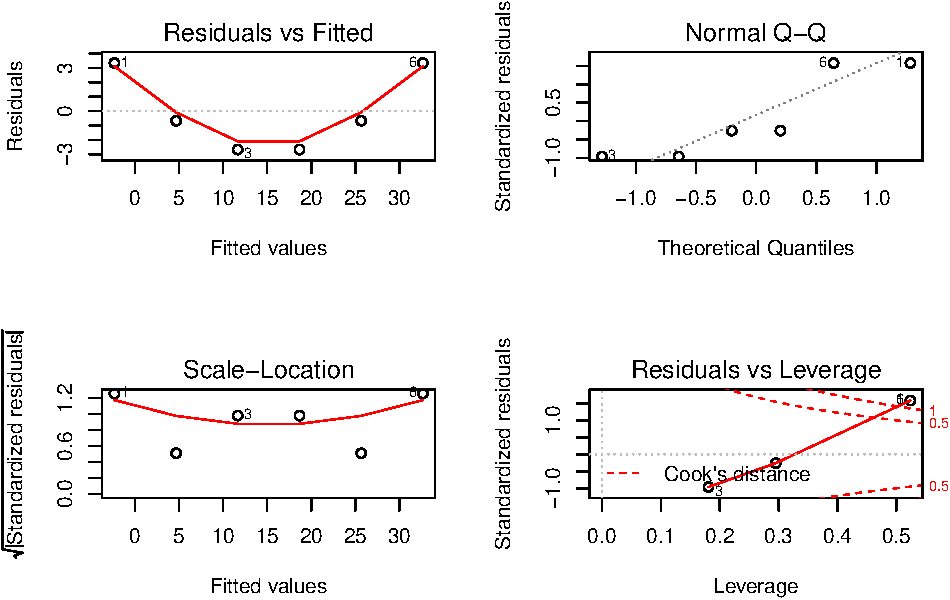
\includegraphics{DASE_files/figure-latex/unnamed-chunk-1-1.pdf} * R
script. \# A file with R commands \texttt{\#\ comments}
\texttt{source("filewithcommands.R")}
\texttt{sink("recordmycommands.lis")} \texttt{savehistory()} * From
command line: + Rscript\\
+ Rscript file with \texttt{-e} (e.g. \texttt{Rscript\ -e\ 2+2})\\
+ To exit R: \texttt{quit()}

\begin{itemize}
\tightlist
\item
  Variables
\item
  Operators

  \begin{itemize}
  \tightlist
  \item
    assign operator \texttt{\textless{}-}\\
  \item
    sequence operator : Example: \texttt{mynums\ \textless{}-\ 0:20}
  \item
    arithmetic operators: + - = / \^{} \%/\% (integer division) \%\%
    (modulus operator)
  \end{itemize}
\item
  The workspace. Objects.

  \begin{itemize}
  \tightlist
  \item
    \texttt{ls()} \texttt{objects()} \texttt{ls.str()} lists and
    describes the objects\\
  \item
    \texttt{rm(x)} delete a variable. E.g., \texttt{rm(totalCost)}
  \item
    \texttt{s.str()}
  \item
    \texttt{objects()}
  \item
    \texttt{str()} The structure function provides information about the
    variable
  \end{itemize}
\item
  RStudio, RCommander and RKWard are the well-known IDEs for R (more
  later).
\end{itemize}

\begin{center}\rule{0.5\linewidth}{\linethickness}\end{center}

\begin{itemize}
\tightlist
\item
  Four \# (`\#\#\#\#') create an \emph{environment} in RStudio. An
  environment binds a set of names to a set of values. You can think of
  an environment as a bag of names.

  \begin{itemize}
  \tightlist
  \item
    \href{http://adv-r.had.co.nz/Environments.html\#env-basics}{Environment
    basics}
  \end{itemize}
\end{itemize}

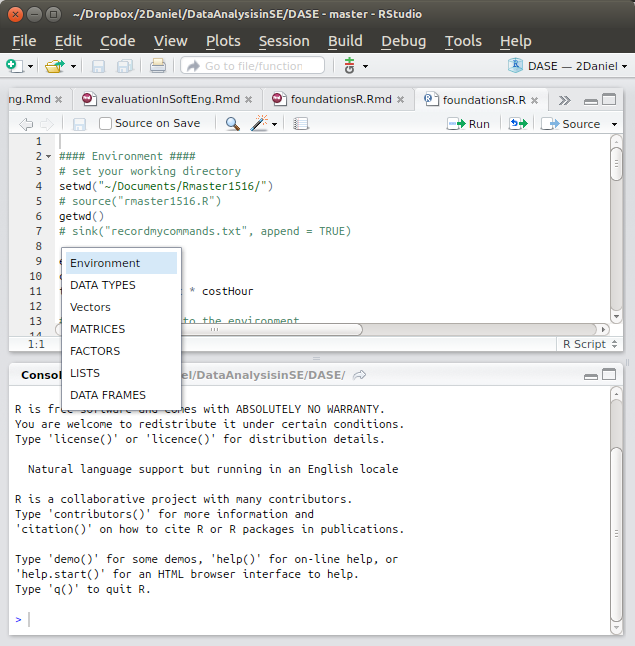
\includegraphics[width=0.75\linewidth]{figures/environments}

Working directories:

\begin{Shaded}
\begin{Highlighting}[]
\CommentTok{# set your working directory}
\CommentTok{# setwd("~/workingDir/")}
\KeywordTok{getwd}\NormalTok{()}
\end{Highlighting}
\end{Shaded}

\begin{verbatim}
## [1] "/home/drg/Projects/DASE"
\end{verbatim}

\begin{Shaded}
\begin{Highlighting}[]
\CommentTok{# record R commands:}
\CommentTok{# sink("recordmycommands.txt", append = TRUE)}
\end{Highlighting}
\end{Shaded}

\begin{center}\rule{0.5\linewidth}{\linethickness}\end{center}

\section{Basic Data Types}\label{basic-data-types}

\begin{itemize}
\tightlist
\item
  class( )
\item
  logical: TRUE FALSE
\item
  numeric, integer:

  \begin{itemize}
  \tightlist
  \item
    is.numeric( )
  \item
    is.integer( )\\
  \end{itemize}
\item
  character
\end{itemize}

Examples:

\begin{Shaded}
\begin{Highlighting}[]
\OtherTok{TRUE}
\end{Highlighting}
\end{Shaded}

\begin{verbatim}
## [1] TRUE
\end{verbatim}

\begin{Shaded}
\begin{Highlighting}[]
\KeywordTok{class}\NormalTok{(}\OtherTok{TRUE}\NormalTok{)}
\end{Highlighting}
\end{Shaded}

\begin{verbatim}
## [1] "logical"
\end{verbatim}

\begin{Shaded}
\begin{Highlighting}[]
\OtherTok{FALSE}
\end{Highlighting}
\end{Shaded}

\begin{verbatim}
## [1] FALSE
\end{verbatim}

\begin{Shaded}
\begin{Highlighting}[]
\OtherTok{NA}  \CommentTok{# missing}
\end{Highlighting}
\end{Shaded}

\begin{verbatim}
## [1] NA
\end{verbatim}

\begin{Shaded}
\begin{Highlighting}[]
\KeywordTok{class}\NormalTok{(}\OtherTok{NA}\NormalTok{)}
\end{Highlighting}
\end{Shaded}

\begin{verbatim}
## [1] "logical"
\end{verbatim}

\begin{Shaded}
\begin{Highlighting}[]
\NormalTok{T}
\end{Highlighting}
\end{Shaded}

\begin{verbatim}
## [1] TRUE
\end{verbatim}

\begin{Shaded}
\begin{Highlighting}[]
\NormalTok{F}
\end{Highlighting}
\end{Shaded}

\begin{verbatim}
## [1] FALSE
\end{verbatim}

\begin{Shaded}
\begin{Highlighting}[]
\CommentTok{# numeric data type}
\DecValTok{2}
\end{Highlighting}
\end{Shaded}

\begin{verbatim}
## [1] 2
\end{verbatim}

\begin{Shaded}
\begin{Highlighting}[]
\KeywordTok{class}\NormalTok{(}\DecValTok{2}\NormalTok{)}
\end{Highlighting}
\end{Shaded}

\begin{verbatim}
## [1] "numeric"
\end{verbatim}

\begin{Shaded}
\begin{Highlighting}[]
\FloatTok{2.5}
\end{Highlighting}
\end{Shaded}

\begin{verbatim}
## [1] 2.5
\end{verbatim}

\begin{Shaded}
\begin{Highlighting}[]
\NormalTok{2L  }\CommentTok{# integer}
\end{Highlighting}
\end{Shaded}

\begin{verbatim}
## [1] 2
\end{verbatim}

\begin{Shaded}
\begin{Highlighting}[]
\KeywordTok{class}\NormalTok{(2L)}
\end{Highlighting}
\end{Shaded}

\begin{verbatim}
## [1] "integer"
\end{verbatim}

\begin{Shaded}
\begin{Highlighting}[]
\KeywordTok{is.numeric}\NormalTok{(}\DecValTok{2}\NormalTok{)}
\end{Highlighting}
\end{Shaded}

\begin{verbatim}
## [1] TRUE
\end{verbatim}

\begin{Shaded}
\begin{Highlighting}[]
\KeywordTok{is.numeric}\NormalTok{(2L)}
\end{Highlighting}
\end{Shaded}

\begin{verbatim}
## [1] TRUE
\end{verbatim}

\begin{Shaded}
\begin{Highlighting}[]
\KeywordTok{is.integer}\NormalTok{(}\DecValTok{2}\NormalTok{)}
\end{Highlighting}
\end{Shaded}

\begin{verbatim}
## [1] FALSE
\end{verbatim}

\begin{Shaded}
\begin{Highlighting}[]
\KeywordTok{is.integer}\NormalTok{(2L)}
\end{Highlighting}
\end{Shaded}

\begin{verbatim}
## [1] TRUE
\end{verbatim}

\begin{itemize}
\tightlist
\item
  data type coercion:

  \begin{itemize}
  \tightlist
  \item
    as.numeric( )
  \item
    as.character( )\\
  \item
    as.integer( )
  \end{itemize}
\end{itemize}

Examples:

\begin{Shaded}
\begin{Highlighting}[]
\NormalTok{truenum <-}\StringTok{ }\KeywordTok{as.numeric}\NormalTok{(}\OtherTok{TRUE}\NormalTok{)}
\NormalTok{truenum}
\end{Highlighting}
\end{Shaded}

\begin{verbatim}
## [1] 1
\end{verbatim}

\begin{Shaded}
\begin{Highlighting}[]
\KeywordTok{class}\NormalTok{(truenum)}
\end{Highlighting}
\end{Shaded}

\begin{verbatim}
## [1] "numeric"
\end{verbatim}

\begin{Shaded}
\begin{Highlighting}[]
\NormalTok{falsenum <-}\StringTok{ }\KeywordTok{as.numeric}\NormalTok{(}\OtherTok{FALSE}\NormalTok{)}
\NormalTok{falsenum}
\end{Highlighting}
\end{Shaded}

\begin{verbatim}
## [1] 0
\end{verbatim}

\begin{Shaded}
\begin{Highlighting}[]
\NormalTok{num2char <-}\StringTok{ }\KeywordTok{as.character}\NormalTok{(}\DecValTok{55}\NormalTok{)}
\NormalTok{num2char}
\end{Highlighting}
\end{Shaded}

\begin{verbatim}
## [1] "55"
\end{verbatim}

\begin{Shaded}
\begin{Highlighting}[]
\NormalTok{char2num  <-}\StringTok{ }\KeywordTok{as.numeric}\NormalTok{(}\StringTok{"55.3"}\NormalTok{)}

\NormalTok{char2int  <-}\StringTok{ }\KeywordTok{as.integer}\NormalTok{(}\StringTok{"55.3"}\NormalTok{)}
\end{Highlighting}
\end{Shaded}

\subsection{Mising values}\label{mising-values}

\begin{itemize}
\tightlist
\item
  NA Not Available, which is not a number as well. It applies to missing
  values.
\item
  NaN means `Not a Number'
\end{itemize}

Examples:

\begin{Shaded}
\begin{Highlighting}[]
\OtherTok{NA} \NormalTok{+}\StringTok{ }\DecValTok{1}
\end{Highlighting}
\end{Shaded}

\begin{verbatim}
## [1] NA
\end{verbatim}

\begin{Shaded}
\begin{Highlighting}[]
\KeywordTok{mean}\NormalTok{(}\KeywordTok{c}\NormalTok{(}\DecValTok{5}\NormalTok{,}\OtherTok{NA}\NormalTok{,}\DecValTok{7}\NormalTok{))}
\end{Highlighting}
\end{Shaded}

\begin{verbatim}
## [1] NA
\end{verbatim}

\begin{Shaded}
\begin{Highlighting}[]
\KeywordTok{mean}\NormalTok{(}\KeywordTok{c}\NormalTok{(}\DecValTok{5}\NormalTok{,}\OtherTok{NA}\NormalTok{,}\DecValTok{7}\NormalTok{), }\DataTypeTok{na.rm=}\OtherTok{TRUE}\NormalTok{)  }\CommentTok{# some functions allow to remove NAs}
\end{Highlighting}
\end{Shaded}

\begin{verbatim}
## [1] 6
\end{verbatim}

\begin{center}\rule{0.5\linewidth}{\linethickness}\end{center}

\section{Vectors}\label{vectors}

Examples:

\begin{Shaded}
\begin{Highlighting}[]
\NormalTok{phases <-}\StringTok{ }\KeywordTok{c}\NormalTok{(}\StringTok{"reqs"}\NormalTok{, }\StringTok{"dev"}\NormalTok{, }\StringTok{"test1"}\NormalTok{, }\StringTok{"test2"}\NormalTok{, }\StringTok{"maint"}\NormalTok{)}
\KeywordTok{str}\NormalTok{(phases)}
\end{Highlighting}
\end{Shaded}

\begin{verbatim}
##  chr [1:5] "reqs" "dev" "test1" "test2" "maint"
\end{verbatim}

\begin{Shaded}
\begin{Highlighting}[]
\KeywordTok{is.vector}\NormalTok{(phases)}
\end{Highlighting}
\end{Shaded}

\begin{verbatim}
## [1] TRUE
\end{verbatim}

\begin{Shaded}
\begin{Highlighting}[]
\NormalTok{thevalues <-}\StringTok{ }\KeywordTok{c}\NormalTok{(}\DecValTok{15}\NormalTok{, }\DecValTok{60}\NormalTok{, }\DecValTok{30}\NormalTok{, }\DecValTok{35}\NormalTok{, }\DecValTok{22}\NormalTok{)}
\KeywordTok{names}\NormalTok{(thevalues) <-}\StringTok{ }\NormalTok{phases}
\KeywordTok{str}\NormalTok{(thevalues)}
\end{Highlighting}
\end{Shaded}

\begin{verbatim}
##  Named num [1:5] 15 60 30 35 22
##  - attr(*, "names")= chr [1:5] "reqs" "dev" "test1" "test2" ...
\end{verbatim}

\begin{Shaded}
\begin{Highlighting}[]
\NormalTok{thevalues}
\end{Highlighting}
\end{Shaded}

\begin{verbatim}
##  reqs   dev test1 test2 maint 
##    15    60    30    35    22
\end{verbatim}

\begin{Shaded}
\begin{Highlighting}[]
\CommentTok{# a single value is a vector}
\NormalTok{aphase <-}\StringTok{ }\DecValTok{44}
\KeywordTok{is.vector}\NormalTok{(aphase)}
\end{Highlighting}
\end{Shaded}

\begin{verbatim}
## [1] TRUE
\end{verbatim}

A single value is a vector! Example:

\begin{Shaded}
\begin{Highlighting}[]
\NormalTok{aphase <-}\StringTok{ }\DecValTok{44}
\KeywordTok{is.vector}\NormalTok{(aphase)}
\end{Highlighting}
\end{Shaded}

\begin{verbatim}
## [1] TRUE
\end{verbatim}

\begin{Shaded}
\begin{Highlighting}[]
\KeywordTok{length}\NormalTok{(aphase)}
\end{Highlighting}
\end{Shaded}

\begin{verbatim}
## [1] 1
\end{verbatim}

\begin{Shaded}
\begin{Highlighting}[]
\KeywordTok{length}\NormalTok{(thevalues)}
\end{Highlighting}
\end{Shaded}

\begin{verbatim}
## [1] 5
\end{verbatim}

\subsection{Coercion for vectors}\label{coercion-for-vectors}

\begin{Shaded}
\begin{Highlighting}[]
\NormalTok{thevalues1 <-}\StringTok{ }\KeywordTok{c}\NormalTok{(}\DecValTok{15}\NormalTok{, }\DecValTok{60}\NormalTok{, }\StringTok{"30"}\NormalTok{, }\DecValTok{35}\NormalTok{, }\DecValTok{22}\NormalTok{)}
\KeywordTok{class}\NormalTok{(thevalues1)}
\end{Highlighting}
\end{Shaded}

\begin{verbatim}
## [1] "character"
\end{verbatim}

\begin{Shaded}
\begin{Highlighting}[]
\NormalTok{thevalues1}
\end{Highlighting}
\end{Shaded}

\begin{verbatim}
## [1] "15" "60" "30" "35" "22"
\end{verbatim}

\begin{Shaded}
\begin{Highlighting}[]
\CommentTok{# <-  is equivalent to   assign ( )}

\KeywordTok{assign}\NormalTok{(}\StringTok{"costs"}\NormalTok{, }\KeywordTok{c}\NormalTok{(}\DecValTok{50}\NormalTok{, }\DecValTok{100}\NormalTok{, }\DecValTok{30}\NormalTok{))}
\end{Highlighting}
\end{Shaded}

\subsection{Vector arithmetic}\label{vector-arithmetic}

It is done in all elements. For example:

\begin{Shaded}
\begin{Highlighting}[]
\KeywordTok{assign}\NormalTok{(}\StringTok{"costs"}\NormalTok{, }\KeywordTok{c}\NormalTok{(}\DecValTok{50}\NormalTok{, }\DecValTok{100}\NormalTok{, }\DecValTok{30}\NormalTok{))}
\NormalTok{costs/}\DecValTok{3}
\end{Highlighting}
\end{Shaded}

\begin{verbatim}
## [1] 16.66667 33.33333 10.00000
\end{verbatim}

\begin{Shaded}
\begin{Highlighting}[]
\NormalTok{costs -}\StringTok{ }\DecValTok{5}
\end{Highlighting}
\end{Shaded}

\begin{verbatim}
## [1] 45 95 25
\end{verbatim}

\begin{Shaded}
\begin{Highlighting}[]
\NormalTok{costs <-}\StringTok{ }\NormalTok{costs -}\StringTok{ }\DecValTok{5}

\NormalTok{incomes <-}\StringTok{ }\KeywordTok{c}\NormalTok{(}\DecValTok{200}\NormalTok{, }\DecValTok{800}\NormalTok{, }\DecValTok{10}\NormalTok{)}
\NormalTok{earnings <-}\StringTok{ }\NormalTok{incomes -}\StringTok{ }\NormalTok{costs}
\KeywordTok{sum}\NormalTok{(earnings)}
\end{Highlighting}
\end{Shaded}

\begin{verbatim}
## [1] 845
\end{verbatim}

\begin{Shaded}
\begin{Highlighting}[]
\CommentTok{# R recycles values in vectors!}
\end{Highlighting}
\end{Shaded}

Subsetting vectors

\begin{Shaded}
\begin{Highlighting}[]
\NormalTok{### Subsetting vectors  []}

\NormalTok{phase1 <-}\StringTok{ }\NormalTok{phases[}\DecValTok{1}\NormalTok{]}
\NormalTok{phase1}
\end{Highlighting}
\end{Shaded}

\begin{verbatim}
## [1] "reqs"
\end{verbatim}

\begin{Shaded}
\begin{Highlighting}[]
\NormalTok{phase3 <-}\StringTok{ }\NormalTok{phases[}\DecValTok{3}\NormalTok{]}
\NormalTok{phase3}
\end{Highlighting}
\end{Shaded}

\begin{verbatim}
## [1] "test1"
\end{verbatim}

\begin{Shaded}
\begin{Highlighting}[]
\NormalTok{thevalues[phase1]}
\end{Highlighting}
\end{Shaded}

\begin{verbatim}
## reqs 
##   15
\end{verbatim}

\begin{Shaded}
\begin{Highlighting}[]
\NormalTok{thevalues[}\StringTok{"reqs"}\NormalTok{]}
\end{Highlighting}
\end{Shaded}

\begin{verbatim}
## reqs 
##   15
\end{verbatim}

\begin{Shaded}
\begin{Highlighting}[]
\NormalTok{testphases <-}\StringTok{ }\NormalTok{phases[}\KeywordTok{c}\NormalTok{(}\DecValTok{3}\NormalTok{,}\DecValTok{4}\NormalTok{)]}
\NormalTok{thevalues[testphases]}
\end{Highlighting}
\end{Shaded}

\begin{verbatim}
## test1 test2 
##    30    35
\end{verbatim}

\begin{Shaded}
\begin{Highlighting}[]
\NormalTok{### Negative indexes}

\NormalTok{phases1 <-}\StringTok{ }\NormalTok{phases[-}\DecValTok{5}\NormalTok{]}
\NormalTok{phases}
\end{Highlighting}
\end{Shaded}

\begin{verbatim}
## [1] "reqs"  "dev"   "test1" "test2" "maint"
\end{verbatim}

\begin{Shaded}
\begin{Highlighting}[]
\NormalTok{phases1}
\end{Highlighting}
\end{Shaded}

\begin{verbatim}
## [1] "reqs"  "dev"   "test1" "test2"
\end{verbatim}

\begin{Shaded}
\begin{Highlighting}[]
\CommentTok{#phases2 <- phases[-testphases] ## error in argument}
\NormalTok{phases2 <-}\StringTok{ }\NormalTok{phases[-}\KeywordTok{c}\NormalTok{(}\DecValTok{3}\NormalTok{,}\DecValTok{4}\NormalTok{)]}
\NormalTok{phases2}
\end{Highlighting}
\end{Shaded}

\begin{verbatim}
## [1] "reqs"  "dev"   "maint"
\end{verbatim}

\begin{Shaded}
\begin{Highlighting}[]
\NormalTok{### subset using logical vector}

\NormalTok{phases3 <-}\StringTok{ }\NormalTok{phases[}\KeywordTok{c}\NormalTok{(}\OtherTok{FALSE}\NormalTok{, }\OtherTok{TRUE}\NormalTok{, }\OtherTok{TRUE}\NormalTok{, }\OtherTok{FALSE}\NormalTok{)] }\CommentTok{#recicled first value}
\NormalTok{phases3}
\end{Highlighting}
\end{Shaded}

\begin{verbatim}
## [1] "dev"   "test1"
\end{verbatim}

\begin{Shaded}
\begin{Highlighting}[]
\NormalTok{selectionv <-}\StringTok{ }\KeywordTok{c}\NormalTok{(}\OtherTok{FALSE}\NormalTok{, }\OtherTok{TRUE}\NormalTok{, }\OtherTok{TRUE}\NormalTok{, }\OtherTok{FALSE}\NormalTok{)}
\NormalTok{phases3 <-}\StringTok{ }\NormalTok{phases[selectionv]}
\NormalTok{phases3}
\end{Highlighting}
\end{Shaded}

\begin{verbatim}
## [1] "dev"   "test1"
\end{verbatim}

\begin{Shaded}
\begin{Highlighting}[]
\NormalTok{selectionvec2 <-}\StringTok{ }\KeywordTok{c}\NormalTok{(}\OtherTok{TRUE}\NormalTok{, }\OtherTok{FALSE}\NormalTok{)}

\NormalTok{thevalues2 <-}\StringTok{ }\NormalTok{thevalues[selectionvec2]}
\NormalTok{thevalues2}
\end{Highlighting}
\end{Shaded}

\begin{verbatim}
##  reqs test1 maint 
##    15    30    22
\end{verbatim}

\begin{Shaded}
\begin{Highlighting}[]
\NormalTok{### Generating regular sequenceswith  : and seq}

\NormalTok{aseqofvalues <-}\StringTok{ }\DecValTok{1}\NormalTok{:}\DecValTok{20}

\NormalTok{aseqofvalues2 <-}\StringTok{ }\KeywordTok{seq}\NormalTok{(}\DataTypeTok{from=}\NormalTok{-}\DecValTok{3}\NormalTok{, }\DataTypeTok{to=}\DecValTok{3}\NormalTok{, }\DataTypeTok{by=}\FloatTok{0.5} \NormalTok{)}
\NormalTok{aseqofvalues2}
\end{Highlighting}
\end{Shaded}

\begin{verbatim}
##  [1] -3.0 -2.5 -2.0 -1.5 -1.0 -0.5  0.0  0.5  1.0  1.5  2.0  2.5  3.0
\end{verbatim}

\begin{Shaded}
\begin{Highlighting}[]
\NormalTok{aseqofvalues3 <-}\StringTok{ }\KeywordTok{seq}\NormalTok{(}\DecValTok{0}\NormalTok{, }\DecValTok{100}\NormalTok{, }\DataTypeTok{by=}\DecValTok{10}\NormalTok{)}
\NormalTok{aseqofvalues4 <-}\StringTok{ }\NormalTok{aseqofvalues3[}\KeywordTok{c}\NormalTok{(}\DecValTok{2}\NormalTok{, }\DecValTok{4}\NormalTok{, }\DecValTok{6}\NormalTok{, }\DecValTok{8}\NormalTok{)]}
\NormalTok{aseqofvalues4}
\end{Highlighting}
\end{Shaded}

\begin{verbatim}
## [1] 10 30 50 70
\end{verbatim}

\begin{Shaded}
\begin{Highlighting}[]
\NormalTok{aseqofvalues4 <-}\StringTok{ }\NormalTok{aseqofvalues3[-}\KeywordTok{c}\NormalTok{(}\DecValTok{2}\NormalTok{, }\DecValTok{4}\NormalTok{, }\DecValTok{6}\NormalTok{, }\DecValTok{8}\NormalTok{)]}
\NormalTok{aseqofvalues4}
\end{Highlighting}
\end{Shaded}

\begin{verbatim}
## [1]   0  20  40  60  80  90 100
\end{verbatim}

\begin{Shaded}
\begin{Highlighting}[]
\NormalTok{aseqofvalues3[}\KeywordTok{c}\NormalTok{(}\DecValTok{1}\NormalTok{,}\DecValTok{2}\NormalTok{)] <-}\StringTok{ }\KeywordTok{c}\NormalTok{(}\DecValTok{666}\NormalTok{,}\DecValTok{888}\NormalTok{)}
\NormalTok{aseqofvalues3}
\end{Highlighting}
\end{Shaded}

\begin{verbatim}
##  [1] 666 888  20  30  40  50  60  70  80  90 100
\end{verbatim}

\begin{Shaded}
\begin{Highlighting}[]
\NormalTok{### Logical values in vectors TRUE/FALSE}

\NormalTok{aseqofvalues3 >}\StringTok{ }\DecValTok{50}
\end{Highlighting}
\end{Shaded}

\begin{verbatim}
##  [1]  TRUE  TRUE FALSE FALSE FALSE FALSE  TRUE  TRUE  TRUE  TRUE  TRUE
\end{verbatim}

\begin{Shaded}
\begin{Highlighting}[]
\NormalTok{aseqofvalues5 <-}\StringTok{ }\NormalTok{aseqofvalues3[aseqofvalues3 >}\StringTok{ }\DecValTok{50}\NormalTok{]}
\NormalTok{aseqofvalues5}
\end{Highlighting}
\end{Shaded}

\begin{verbatim}
## [1] 666 888  60  70  80  90 100
\end{verbatim}

\begin{Shaded}
\begin{Highlighting}[]
\NormalTok{aseqofvalues6 <-}\StringTok{ }\NormalTok{aseqofvalues3[!(aseqofvalues3 >}\StringTok{ }\DecValTok{50}\NormalTok{)]}
\NormalTok{aseqofvalues6}
\end{Highlighting}
\end{Shaded}

\begin{verbatim}
## [1] 20 30 40 50
\end{verbatim}

\begin{Shaded}
\begin{Highlighting}[]
\NormalTok{### Comparison functions}

\NormalTok{aseqofvalues7 <-}\StringTok{ }\NormalTok{aseqofvalues3[aseqofvalues3 ==}\StringTok{ }\DecValTok{50}\NormalTok{]}
\NormalTok{aseqofvalues7}
\end{Highlighting}
\end{Shaded}

\begin{verbatim}
## [1] 50
\end{verbatim}

\begin{Shaded}
\begin{Highlighting}[]
\NormalTok{aseqofvalues8 <-}\StringTok{ }\NormalTok{aseqofvalues3[aseqofvalues3 ==}\StringTok{ }\DecValTok{22}\NormalTok{]}
\NormalTok{aseqofvalues8}
\end{Highlighting}
\end{Shaded}

\begin{verbatim}
## numeric(0)
\end{verbatim}

\begin{Shaded}
\begin{Highlighting}[]
\NormalTok{aseqofvalues9 <-}\StringTok{ }\NormalTok{aseqofvalues3[aseqofvalues3 !=}\StringTok{ }\DecValTok{50}\NormalTok{]}
\NormalTok{aseqofvalues9}
\end{Highlighting}
\end{Shaded}

\begin{verbatim}
##  [1] 666 888  20  30  40  60  70  80  90 100
\end{verbatim}

\begin{Shaded}
\begin{Highlighting}[]
\NormalTok{logicalcond <-}\StringTok{ }\NormalTok{aseqofvalues3 >=}\StringTok{ }\DecValTok{50}
\NormalTok{aseqofvalues10 <-}\StringTok{ }\NormalTok{aseqofvalues3[logicalcond]}
\NormalTok{aseqofvalues10}
\end{Highlighting}
\end{Shaded}

\begin{verbatim}
## [1] 666 888  50  60  70  80  90 100
\end{verbatim}

\begin{Shaded}
\begin{Highlighting}[]
\NormalTok{### Remove Missing Values (NAs)}

\NormalTok{aseqofvalues3[}\KeywordTok{c}\NormalTok{(}\DecValTok{1}\NormalTok{,}\DecValTok{2}\NormalTok{)] <-}\StringTok{ }\KeywordTok{c}\NormalTok{(}\OtherTok{NA}\NormalTok{,}\OtherTok{NA}\NormalTok{)}
\NormalTok{aseqofvalues3}
\end{Highlighting}
\end{Shaded}

\begin{verbatim}
##  [1]  NA  NA  20  30  40  50  60  70  80  90 100
\end{verbatim}

\begin{Shaded}
\begin{Highlighting}[]
\NormalTok{aseqofvalues3 <-}\StringTok{ }\NormalTok{aseqofvalues3[!}\KeywordTok{is.na}\NormalTok{(aseqofvalues3)]}
\NormalTok{aseqofvalues3}
\end{Highlighting}
\end{Shaded}

\begin{verbatim}
## [1]  20  30  40  50  60  70  80  90 100
\end{verbatim}

\begin{center}\rule{0.5\linewidth}{\linethickness}\end{center}

\section{Arrays and Matrices}\label{arrays-and-matrices}

\begin{Shaded}
\begin{Highlighting}[]
\NormalTok{mymat <-}\StringTok{ }\KeywordTok{matrix}\NormalTok{(}\DecValTok{1}\NormalTok{:}\DecValTok{12}\NormalTok{, }\DataTypeTok{nrow =}\DecValTok{2}\NormalTok{)}
\NormalTok{mymat}
\end{Highlighting}
\end{Shaded}

\begin{verbatim}
##      [,1] [,2] [,3] [,4] [,5] [,6]
## [1,]    1    3    5    7    9   11
## [2,]    2    4    6    8   10   12
\end{verbatim}

\begin{Shaded}
\begin{Highlighting}[]
\NormalTok{mymat <-}\StringTok{ }\KeywordTok{matrix}\NormalTok{(}\DecValTok{1}\NormalTok{:}\DecValTok{12}\NormalTok{, }\DataTypeTok{ncol =}\DecValTok{3}\NormalTok{)}
\NormalTok{mymat}
\end{Highlighting}
\end{Shaded}

\begin{verbatim}
##      [,1] [,2] [,3]
## [1,]    1    5    9
## [2,]    2    6   10
## [3,]    3    7   11
## [4,]    4    8   12
\end{verbatim}

\begin{Shaded}
\begin{Highlighting}[]
\NormalTok{mymat <-}\StringTok{ }\KeywordTok{matrix}\NormalTok{(}\DecValTok{1}\NormalTok{:}\DecValTok{12}\NormalTok{, }\DataTypeTok{nrow=}\DecValTok{2}\NormalTok{, }\DataTypeTok{byrow =} \OtherTok{TRUE}\NormalTok{)}
\NormalTok{mymat}
\end{Highlighting}
\end{Shaded}

\begin{verbatim}
##      [,1] [,2] [,3] [,4] [,5] [,6]
## [1,]    1    2    3    4    5    6
## [2,]    7    8    9   10   11   12
\end{verbatim}

\begin{Shaded}
\begin{Highlighting}[]
\NormalTok{mymat <-}\StringTok{ }\KeywordTok{matrix}\NormalTok{(}\DecValTok{1}\NormalTok{:}\DecValTok{12}\NormalTok{, }\DataTypeTok{nrow=}\DecValTok{3}\NormalTok{, }\DataTypeTok{ncol=}\DecValTok{4}\NormalTok{)}
\NormalTok{mymat}
\end{Highlighting}
\end{Shaded}

\begin{verbatim}
##      [,1] [,2] [,3] [,4]
## [1,]    1    4    7   10
## [2,]    2    5    8   11
## [3,]    3    6    9   12
\end{verbatim}

\begin{Shaded}
\begin{Highlighting}[]
\NormalTok{mymat <-}\StringTok{ }\KeywordTok{matrix}\NormalTok{(}\DecValTok{1}\NormalTok{:}\DecValTok{12}\NormalTok{, }\DataTypeTok{nrow=}\DecValTok{3}\NormalTok{, }\DataTypeTok{ncol=}\DecValTok{4}\NormalTok{, }\DataTypeTok{byrow=}\OtherTok{TRUE}\NormalTok{)}
\NormalTok{mymat}
\end{Highlighting}
\end{Shaded}

\begin{verbatim}
##      [,1] [,2] [,3] [,4]
## [1,]    1    2    3    4
## [2,]    5    6    7    8
## [3,]    9   10   11   12
\end{verbatim}

\begin{Shaded}
\begin{Highlighting}[]
\NormalTok{### recycling}
\NormalTok{mymat <-}\StringTok{ }\KeywordTok{matrix}\NormalTok{(}\DecValTok{1}\NormalTok{:}\DecValTok{5}\NormalTok{, }\DataTypeTok{nrow=}\DecValTok{3}\NormalTok{, }\DataTypeTok{ncol=}\DecValTok{4}\NormalTok{, }\DataTypeTok{byrow=}\OtherTok{TRUE}\NormalTok{)}
\end{Highlighting}
\end{Shaded}

\begin{verbatim}
## Warning in matrix(1:5, nrow = 3, ncol = 4, byrow = TRUE): data length [5]
## is not a sub-multiple or multiple of the number of rows [3]
\end{verbatim}

\begin{Shaded}
\begin{Highlighting}[]
\NormalTok{mymat}
\end{Highlighting}
\end{Shaded}

\begin{verbatim}
##      [,1] [,2] [,3] [,4]
## [1,]    1    2    3    4
## [2,]    5    1    2    3
## [3,]    4    5    1    2
\end{verbatim}

\begin{Shaded}
\begin{Highlighting}[]
\NormalTok{### rbind  cbind}

\KeywordTok{cbind}\NormalTok{(}\DecValTok{1}\NormalTok{:}\DecValTok{3}\NormalTok{, }\DecValTok{1}\NormalTok{:}\DecValTok{3}\NormalTok{)}
\end{Highlighting}
\end{Shaded}

\begin{verbatim}
##      [,1] [,2]
## [1,]    1    1
## [2,]    2    2
## [3,]    3    3
\end{verbatim}

\begin{Shaded}
\begin{Highlighting}[]
\KeywordTok{rbind}\NormalTok{(}\DecValTok{1}\NormalTok{:}\DecValTok{3}\NormalTok{, }\DecValTok{1}\NormalTok{:}\DecValTok{3}\NormalTok{)}
\end{Highlighting}
\end{Shaded}

\begin{verbatim}
##      [,1] [,2] [,3]
## [1,]    1    2    3
## [2,]    1    2    3
\end{verbatim}

\begin{Shaded}
\begin{Highlighting}[]
\NormalTok{mymat <-}\StringTok{ }\KeywordTok{matrix}\NormalTok{(}\DecValTok{1}\NormalTok{)}

\NormalTok{mymat <-}\StringTok{ }\KeywordTok{matrix}\NormalTok{(}\DecValTok{1}\NormalTok{:}\DecValTok{8}\NormalTok{, }\DataTypeTok{nrow=}\DecValTok{2}\NormalTok{, }\DataTypeTok{ncol=}\DecValTok{4}\NormalTok{, }\DataTypeTok{byrow=}\OtherTok{TRUE}\NormalTok{)}
\NormalTok{mymat}
\end{Highlighting}
\end{Shaded}

\begin{verbatim}
##      [,1] [,2] [,3] [,4]
## [1,]    1    2    3    4
## [2,]    5    6    7    8
\end{verbatim}

\begin{Shaded}
\begin{Highlighting}[]
\KeywordTok{rbind}\NormalTok{(mymat, }\DecValTok{9}\NormalTok{:}\DecValTok{12}\NormalTok{)}
\end{Highlighting}
\end{Shaded}

\begin{verbatim}
##      [,1] [,2] [,3] [,4]
## [1,]    1    2    3    4
## [2,]    5    6    7    8
## [3,]    9   10   11   12
\end{verbatim}

\begin{Shaded}
\begin{Highlighting}[]
\NormalTok{mymat <-}\StringTok{ }\KeywordTok{cbind}\NormalTok{(mymat, }\KeywordTok{c}\NormalTok{(}\DecValTok{5}\NormalTok{,}\DecValTok{9}\NormalTok{))}
\NormalTok{mymat}
\end{Highlighting}
\end{Shaded}

\begin{verbatim}
##      [,1] [,2] [,3] [,4] [,5]
## [1,]    1    2    3    4    5
## [2,]    5    6    7    8    9
\end{verbatim}

\begin{Shaded}
\begin{Highlighting}[]
\NormalTok{mymat  <-}\StringTok{ }\KeywordTok{matrix}\NormalTok{(}\DecValTok{1}\NormalTok{:}\DecValTok{8}\NormalTok{, }\DataTypeTok{byrow =} \OtherTok{TRUE}\NormalTok{, }\DataTypeTok{nrow=}\DecValTok{2}\NormalTok{)}
\NormalTok{mymat}
\end{Highlighting}
\end{Shaded}

\begin{verbatim}
##      [,1] [,2] [,3] [,4]
## [1,]    1    2    3    4
## [2,]    5    6    7    8
\end{verbatim}

\begin{Shaded}
\begin{Highlighting}[]
\KeywordTok{rownames}\NormalTok{(mymat) <-}\StringTok{ }\KeywordTok{c}\NormalTok{(}\StringTok{"row1"}\NormalTok{, }\StringTok{"row2"}\NormalTok{)}
\NormalTok{mymat}
\end{Highlighting}
\end{Shaded}

\begin{verbatim}
##      [,1] [,2] [,3] [,4]
## row1    1    2    3    4
## row2    5    6    7    8
\end{verbatim}

\begin{Shaded}
\begin{Highlighting}[]
\KeywordTok{colnames}\NormalTok{(mymat) <-}\StringTok{ }\KeywordTok{c}\NormalTok{(}\StringTok{"col1"}\NormalTok{, }\StringTok{"col2"}\NormalTok{, }\StringTok{"col3"}\NormalTok{, }\StringTok{"col4"}\NormalTok{)}
\NormalTok{mymat}
\end{Highlighting}
\end{Shaded}

\begin{verbatim}
##      col1 col2 col3 col4
## row1    1    2    3    4
## row2    5    6    7    8
\end{verbatim}

\begin{Shaded}
\begin{Highlighting}[]
\NormalTok{mymat2 <-}\StringTok{ }\KeywordTok{matrix}\NormalTok{(}\DecValTok{1}\NormalTok{:}\DecValTok{12}\NormalTok{, }\DataTypeTok{byrow=}\OtherTok{TRUE}\NormalTok{, }\DataTypeTok{nrow=}\DecValTok{3}\NormalTok{, }\DataTypeTok{dimnames=}\KeywordTok{list}\NormalTok{(}\KeywordTok{c}\NormalTok{(}\StringTok{"row1"}\NormalTok{, }\StringTok{"row2"}\NormalTok{, }\StringTok{"row3"}\NormalTok{),}
                                                         \KeywordTok{c}\NormalTok{(}\StringTok{"col1"}\NormalTok{, }\StringTok{"col2"}\NormalTok{, }\StringTok{"col3"}\NormalTok{, }\StringTok{"col4"}\NormalTok{)))}
\NormalTok{mymat2}
\end{Highlighting}
\end{Shaded}

\begin{verbatim}
##      col1 col2 col3 col4
## row1    1    2    3    4
## row2    5    6    7    8
## row3    9   10   11   12
\end{verbatim}

\begin{Shaded}
\begin{Highlighting}[]
\NormalTok{### Coercion in Arrays}

\NormalTok{matnum <-}\StringTok{ }\KeywordTok{matrix}\NormalTok{(}\DecValTok{1}\NormalTok{:}\DecValTok{8}\NormalTok{, }\DataTypeTok{ncol =} \DecValTok{2}\NormalTok{)}
\NormalTok{matnum}
\end{Highlighting}
\end{Shaded}

\begin{verbatim}
##      [,1] [,2]
## [1,]    1    5
## [2,]    2    6
## [3,]    3    7
## [4,]    4    8
\end{verbatim}

\begin{Shaded}
\begin{Highlighting}[]
\NormalTok{matchar <-}\StringTok{ }\KeywordTok{matrix}\NormalTok{(LETTERS[}\DecValTok{1}\NormalTok{:}\DecValTok{6}\NormalTok{], }\DataTypeTok{nrow =} \DecValTok{4}\NormalTok{, }\DataTypeTok{ncol =} \DecValTok{3}\NormalTok{)}
\NormalTok{matchar}
\end{Highlighting}
\end{Shaded}

\begin{verbatim}
##      [,1] [,2] [,3]
## [1,] "A"  "E"  "C" 
## [2,] "B"  "F"  "D" 
## [3,] "C"  "A"  "E" 
## [4,] "D"  "B"  "F"
\end{verbatim}

\begin{Shaded}
\begin{Highlighting}[]
\NormalTok{matchars <-}\StringTok{ }\KeywordTok{cbind}\NormalTok{(matnum, matchar)}
\NormalTok{matchars}
\end{Highlighting}
\end{Shaded}

\begin{verbatim}
##      [,1] [,2] [,3] [,4] [,5]
## [1,] "1"  "5"  "A"  "E"  "C" 
## [2,] "2"  "6"  "B"  "F"  "D" 
## [3,] "3"  "7"  "C"  "A"  "E" 
## [4,] "4"  "8"  "D"  "B"  "F"
\end{verbatim}

\begin{Shaded}
\begin{Highlighting}[]
\NormalTok{### Subsetting  }

\NormalTok{mymat3 <-}\StringTok{ }\KeywordTok{matrix}\NormalTok{(}\KeywordTok{sample}\NormalTok{(-}\DecValTok{8}\NormalTok{:}\DecValTok{15}\NormalTok{, }\DecValTok{12}\NormalTok{), }\DataTypeTok{nrow=}\DecValTok{3}\NormalTok{)}
\NormalTok{mymat3}
\end{Highlighting}
\end{Shaded}

\begin{verbatim}
##      [,1] [,2] [,3] [,4]
## [1,]    6   -6    0   11
## [2,]   -3   -1   -4    1
## [3,]   -7   -2   13    2
\end{verbatim}

\begin{Shaded}
\begin{Highlighting}[]
\NormalTok{mymat3[}\DecValTok{2}\NormalTok{,}\DecValTok{3}\NormalTok{]}
\end{Highlighting}
\end{Shaded}

\begin{verbatim}
## [1] -4
\end{verbatim}

\begin{Shaded}
\begin{Highlighting}[]
\NormalTok{mymat3[}\DecValTok{1}\NormalTok{,}\DecValTok{4}\NormalTok{]}
\end{Highlighting}
\end{Shaded}

\begin{verbatim}
## [1] 11
\end{verbatim}

\begin{Shaded}
\begin{Highlighting}[]
\NormalTok{mymat3[}\DecValTok{3}\NormalTok{,]}
\end{Highlighting}
\end{Shaded}

\begin{verbatim}
## [1] -7 -2 13  2
\end{verbatim}

\begin{Shaded}
\begin{Highlighting}[]
\NormalTok{mymat3[,}\DecValTok{4}\NormalTok{]}
\end{Highlighting}
\end{Shaded}

\begin{verbatim}
## [1] 11  1  2
\end{verbatim}

\begin{Shaded}
\begin{Highlighting}[]
\NormalTok{mymat3[}\DecValTok{5}\NormalTok{] }\CommentTok{# counts elements by column}
\end{Highlighting}
\end{Shaded}

\begin{verbatim}
## [1] -1
\end{verbatim}

\begin{Shaded}
\begin{Highlighting}[]
\NormalTok{mymat3[}\DecValTok{9}\NormalTok{]}
\end{Highlighting}
\end{Shaded}

\begin{verbatim}
## [1] 13
\end{verbatim}

\begin{Shaded}
\begin{Highlighting}[]
\NormalTok{## Subsetting multiple elements}

\NormalTok{mymat3[}\DecValTok{2}\NormalTok{, }\KeywordTok{c}\NormalTok{(}\DecValTok{1}\NormalTok{,}\DecValTok{3}\NormalTok{)]}
\end{Highlighting}
\end{Shaded}

\begin{verbatim}
## [1] -3 -4
\end{verbatim}

\begin{Shaded}
\begin{Highlighting}[]
\NormalTok{mymat3[}\KeywordTok{c}\NormalTok{(}\DecValTok{2}\NormalTok{,}\DecValTok{3}\NormalTok{), }\KeywordTok{c}\NormalTok{(}\DecValTok{1}\NormalTok{,}\DecValTok{3}\NormalTok{,}\DecValTok{4}\NormalTok{)]}
\end{Highlighting}
\end{Shaded}

\begin{verbatim}
##      [,1] [,2] [,3]
## [1,]   -3   -4    1
## [2,]   -7   13    2
\end{verbatim}

\begin{Shaded}
\begin{Highlighting}[]
\KeywordTok{rownames}\NormalTok{(mymat3) <-}\StringTok{ }\KeywordTok{c}\NormalTok{(}\StringTok{"r1"}\NormalTok{, }\StringTok{"r2"}\NormalTok{, }\StringTok{"r3"}\NormalTok{)}
\KeywordTok{colnames}\NormalTok{(mymat3) <-}\StringTok{ }\KeywordTok{c}\NormalTok{(}\StringTok{"c1"}\NormalTok{, }\StringTok{"c2"}\NormalTok{, }\StringTok{"c3"}\NormalTok{, }\StringTok{"c4"}\NormalTok{)}
\NormalTok{mymat3[}\StringTok{"r2"}\NormalTok{, }\KeywordTok{c}\NormalTok{(}\StringTok{"c1"}\NormalTok{, }\StringTok{"c3"}\NormalTok{)]}
\end{Highlighting}
\end{Shaded}

\begin{verbatim}
## c1 c3 
## -3 -4
\end{verbatim}

\begin{Shaded}
\begin{Highlighting}[]
\NormalTok{### Subset by logical vector}
\NormalTok{mymat3[}\KeywordTok{c}\NormalTok{(}\OtherTok{FALSE}\NormalTok{, }\OtherTok{TRUE}\NormalTok{, }\OtherTok{FALSE}\NormalTok{),}
       \KeywordTok{c}\NormalTok{(}\OtherTok{TRUE}\NormalTok{, }\OtherTok{FALSE}\NormalTok{, }\OtherTok{TRUE}\NormalTok{, }\OtherTok{FALSE}\NormalTok{)]}
\end{Highlighting}
\end{Shaded}

\begin{verbatim}
## c1 c3 
## -3 -4
\end{verbatim}

\begin{Shaded}
\begin{Highlighting}[]
\NormalTok{mymat3[}\KeywordTok{c}\NormalTok{(}\OtherTok{FALSE}\NormalTok{, }\OtherTok{TRUE}\NormalTok{, }\OtherTok{TRUE}\NormalTok{),}
       \KeywordTok{c}\NormalTok{(}\OtherTok{TRUE}\NormalTok{, }\OtherTok{FALSE}\NormalTok{, }\OtherTok{TRUE}\NormalTok{, }\OtherTok{TRUE}\NormalTok{)]}
\end{Highlighting}
\end{Shaded}

\begin{verbatim}
##    c1 c3 c4
## r2 -3 -4  1
## r3 -7 13  2
\end{verbatim}

\begin{Shaded}
\begin{Highlighting}[]
\NormalTok{### matrix arithmetic}

\NormalTok{row1 <-}\StringTok{ }\KeywordTok{c}\NormalTok{(}\DecValTok{220}\NormalTok{, }\DecValTok{137}\NormalTok{)}
\NormalTok{row2 <-}\StringTok{ }\KeywordTok{c}\NormalTok{(}\DecValTok{345}\NormalTok{, }\DecValTok{987}\NormalTok{)}
\NormalTok{row3 <-}\StringTok{ }\KeywordTok{c}\NormalTok{(}\DecValTok{111}\NormalTok{, }\DecValTok{777}\NormalTok{)}

\NormalTok{mymat4 <-}\StringTok{ }\KeywordTok{rbind}\NormalTok{(row1, row2, row3)}
\KeywordTok{rownames}\NormalTok{(mymat4) <-}\StringTok{ }\KeywordTok{c}\NormalTok{(}\StringTok{"row_1"}\NormalTok{, }\StringTok{"row_2"}\NormalTok{, }\StringTok{"row_3"}\NormalTok{)}
\KeywordTok{colnames}\NormalTok{(mymat4) <-}\StringTok{ }\KeywordTok{c}\NormalTok{(}\StringTok{"col_1"}\NormalTok{, }\StringTok{"col_2"}\NormalTok{)}
\NormalTok{mymat4}
\end{Highlighting}
\end{Shaded}

\begin{verbatim}
##       col_1 col_2
## row_1   220   137
## row_2   345   987
## row_3   111   777
\end{verbatim}

\begin{Shaded}
\begin{Highlighting}[]
\NormalTok{mymat4/}\DecValTok{10}
\end{Highlighting}
\end{Shaded}

\begin{verbatim}
##       col_1 col_2
## row_1  22.0  13.7
## row_2  34.5  98.7
## row_3  11.1  77.7
\end{verbatim}

\begin{Shaded}
\begin{Highlighting}[]
\NormalTok{mymat4 -}\DecValTok{100}
\end{Highlighting}
\end{Shaded}

\begin{verbatim}
##       col_1 col_2
## row_1   120    37
## row_2   245   887
## row_3    11   677
\end{verbatim}

\begin{Shaded}
\begin{Highlighting}[]
\NormalTok{mymat5 <-}\StringTok{ }\KeywordTok{rbind}\NormalTok{(}\KeywordTok{c}\NormalTok{(}\DecValTok{50}\NormalTok{,}\DecValTok{50}\NormalTok{), }\KeywordTok{c}\NormalTok{(}\DecValTok{10}\NormalTok{,}\DecValTok{10}\NormalTok{), }\KeywordTok{c}\NormalTok{(}\DecValTok{100}\NormalTok{,}\DecValTok{100}\NormalTok{))}
\NormalTok{mymat5}
\end{Highlighting}
\end{Shaded}

\begin{verbatim}
##      [,1] [,2]
## [1,]   50   50
## [2,]   10   10
## [3,]  100  100
\end{verbatim}

\begin{Shaded}
\begin{Highlighting}[]
\NormalTok{mymat4 -}\StringTok{ }\NormalTok{mymat5}
\end{Highlighting}
\end{Shaded}

\begin{verbatim}
##       col_1 col_2
## row_1   170    87
## row_2   335   977
## row_3    11   677
\end{verbatim}

\begin{Shaded}
\begin{Highlighting}[]
\NormalTok{mymat4 *}\StringTok{ }\NormalTok{(mymat5/}\DecValTok{100}\NormalTok{)}
\end{Highlighting}
\end{Shaded}

\begin{verbatim}
##       col_1 col_2
## row_1 110.0  68.5
## row_2  34.5  98.7
## row_3 111.0 777.0
\end{verbatim}

\begin{Shaded}
\begin{Highlighting}[]
\NormalTok{### index matrices}

\NormalTok{m1 <-}\StringTok{ }\KeywordTok{array}\NormalTok{(}\DecValTok{1}\NormalTok{:}\DecValTok{20}\NormalTok{, }\DataTypeTok{dim=}\KeywordTok{c}\NormalTok{(}\DecValTok{4}\NormalTok{,}\DecValTok{5}\NormalTok{))}
\NormalTok{m1}
\end{Highlighting}
\end{Shaded}

\begin{verbatim}
##      [,1] [,2] [,3] [,4] [,5]
## [1,]    1    5    9   13   17
## [2,]    2    6   10   14   18
## [3,]    3    7   11   15   19
## [4,]    4    8   12   16   20
\end{verbatim}

\begin{Shaded}
\begin{Highlighting}[]
\NormalTok{index <-}\StringTok{ }\KeywordTok{array}\NormalTok{(}\KeywordTok{c}\NormalTok{(}\DecValTok{1}\NormalTok{:}\DecValTok{3}\NormalTok{, }\DecValTok{3}\NormalTok{:}\DecValTok{1}\NormalTok{), }\DataTypeTok{dim=}\KeywordTok{c}\NormalTok{(}\DecValTok{3}\NormalTok{,}\DecValTok{2}\NormalTok{))}
\NormalTok{index}
\end{Highlighting}
\end{Shaded}

\begin{verbatim}
##      [,1] [,2]
## [1,]    1    3
## [2,]    2    2
## [3,]    3    1
\end{verbatim}

\begin{Shaded}
\begin{Highlighting}[]
\NormalTok{m1[index] <-}\DecValTok{0}
\NormalTok{m1}
\end{Highlighting}
\end{Shaded}

\begin{verbatim}
##      [,1] [,2] [,3] [,4] [,5]
## [1,]    1    5    0   13   17
## [2,]    2    0   10   14   18
## [3,]    0    7   11   15   19
## [4,]    4    8   12   16   20
\end{verbatim}

\begin{center}\rule{0.5\linewidth}{\linethickness}\end{center}

\section{Factors}\label{factors}

\begin{itemize}
\tightlist
\item
  Factors in R are stored as a vector of integer values with a
  corresponding set of character values to use when the factor is
  displayed.
\end{itemize}

\begin{Shaded}
\begin{Highlighting}[]
\NormalTok{personnel <-}\StringTok{ }\KeywordTok{c}\NormalTok{(}\StringTok{"Analyst1"}\NormalTok{, }\StringTok{"ManagerL2"}\NormalTok{, }\StringTok{"Analyst1"}\NormalTok{, }\StringTok{"Analyst2"}\NormalTok{,  }\StringTok{"Boss"}\NormalTok{, }\StringTok{"ManagerL1"}\NormalTok{, }\StringTok{"ManagerL2"}\NormalTok{, }\StringTok{"Programmer1"}\NormalTok{, }\StringTok{"Programmer2"}\NormalTok{, }\StringTok{"Programmer3"}\NormalTok{, }\StringTok{"Designer1"}\NormalTok{,}\StringTok{"Designer2"}\NormalTok{, }\StringTok{"OtherStaff"}\NormalTok{)  }\CommentTok{# staff in a company}

\NormalTok{personnel_factors <-}\StringTok{ }\KeywordTok{factor}\NormalTok{(personnel)}
\NormalTok{personnel_factors  }\CommentTok{#sorted alphabetically}
\end{Highlighting}
\end{Shaded}

\begin{verbatim}
##  [1] Analyst1    ManagerL2   Analyst1    Analyst2    Boss       
##  [6] ManagerL1   ManagerL2   Programmer1 Programmer2 Programmer3
## [11] Designer1   Designer2   OtherStaff 
## 11 Levels: Analyst1 Analyst2 Boss Designer1 Designer2 ... Programmer3
\end{verbatim}

\begin{Shaded}
\begin{Highlighting}[]
\KeywordTok{str}\NormalTok{(personnel_factors)}
\end{Highlighting}
\end{Shaded}

\begin{verbatim}
##  Factor w/ 11 levels "Analyst1","Analyst2",..: 1 7 1 2 3 6 7 9 10 11 ...
\end{verbatim}

\begin{Shaded}
\begin{Highlighting}[]
\NormalTok{personnel2 <-}\StringTok{ }\KeywordTok{factor}\NormalTok{(personnel, }
                       \DataTypeTok{levels =} \KeywordTok{c}\NormalTok{(}\StringTok{"Boss"}\NormalTok{, }\StringTok{"ManagerL1"}\NormalTok{, }\StringTok{"ManagerL2"}\NormalTok{, }\StringTok{"Analyst1"}\NormalTok{, }\StringTok{"Analyst2"}\NormalTok{,  }\StringTok{"Designer1"}\NormalTok{,}\StringTok{"Designer2"}\NormalTok{, }\StringTok{"Programmer1"}\NormalTok{, }\StringTok{"Programmer2"}\NormalTok{, }\StringTok{"Programmer3"}\NormalTok{, }\StringTok{"OtherStaff"}\NormalTok{))  }\CommentTok{#do not duplicate the same factors}
\NormalTok{personnel2}
\end{Highlighting}
\end{Shaded}

\begin{verbatim}
##  [1] Analyst1    ManagerL2   Analyst1    Analyst2    Boss       
##  [6] ManagerL1   ManagerL2   Programmer1 Programmer2 Programmer3
## [11] Designer1   Designer2   OtherStaff 
## 11 Levels: Boss ManagerL1 ManagerL2 Analyst1 Analyst2 ... OtherStaff
\end{verbatim}

\begin{Shaded}
\begin{Highlighting}[]
\KeywordTok{str}\NormalTok{(personnel2)}
\end{Highlighting}
\end{Shaded}

\begin{verbatim}
##  Factor w/ 11 levels "Boss","ManagerL1",..: 4 3 4 5 1 2 3 8 9 10 ...
\end{verbatim}

\begin{Shaded}
\begin{Highlighting}[]
\CommentTok{# a factor's levels will always be character values.}

\KeywordTok{levels}\NormalTok{(personnel2) <-}\StringTok{ }\KeywordTok{c}\NormalTok{(}\StringTok{"B"}\NormalTok{, }\StringTok{"M1"}\NormalTok{, }\StringTok{"M2"}\NormalTok{, }\StringTok{"A1"}\NormalTok{, }\StringTok{"A2"}\NormalTok{, }\StringTok{"D1"}\NormalTok{, }\StringTok{"D2"}\NormalTok{, }\StringTok{"P1"}\NormalTok{, }\StringTok{"P2"}\NormalTok{, }\StringTok{"P3"}\NormalTok{, }\StringTok{"OS"}\NormalTok{)}
\NormalTok{personnel2}
\end{Highlighting}
\end{Shaded}

\begin{verbatim}
##  [1] A1 M2 A1 A2 B  M1 M2 P1 P2 P3 D1 D2 OS
## Levels: B M1 M2 A1 A2 D1 D2 P1 P2 P3 OS
\end{verbatim}

\begin{Shaded}
\begin{Highlighting}[]
\NormalTok{personnel3 <-}\StringTok{ }\KeywordTok{factor}\NormalTok{(personnel,}
                     \DataTypeTok{levels =} \KeywordTok{c}\NormalTok{(}\StringTok{"Boss"}\NormalTok{, }\StringTok{"ManagerL1"}\NormalTok{, }\StringTok{"ManagerL2"}\NormalTok{, }\StringTok{"Analyst1"}\NormalTok{, }\StringTok{"Analyst2"}\NormalTok{,  }\StringTok{"Designer1"}\NormalTok{,}\StringTok{"Designer2"}\NormalTok{, }\StringTok{"Programmer1"}\NormalTok{, }\StringTok{"Programmer2"}\NormalTok{, }\StringTok{"Programmer3"}\NormalTok{, }\StringTok{"OtherStaff"}\NormalTok{),}
                     \KeywordTok{c}\NormalTok{(}\StringTok{"B"}\NormalTok{, }\StringTok{"M1"}\NormalTok{, }\StringTok{"M2"}\NormalTok{, }\StringTok{"A1"}\NormalTok{, }\StringTok{"A2"}\NormalTok{, }\StringTok{"D1"}\NormalTok{, }\StringTok{"D2"}\NormalTok{, }\StringTok{"P1"}\NormalTok{, }\StringTok{"P2"}\NormalTok{, }\StringTok{"P3"}\NormalTok{, }\StringTok{"OS"}\NormalTok{))}
\NormalTok{personnel3}
\end{Highlighting}
\end{Shaded}

\begin{verbatim}
##  [1] A1 M2 A1 A2 B  M1 M2 P1 P2 P3 D1 D2 OS
## Levels: B M1 M2 A1 A2 D1 D2 P1 P2 P3 OS
\end{verbatim}

\begin{Shaded}
\begin{Highlighting}[]
\NormalTok{### Nominal versus ordinal, ordered factors}
\NormalTok{personnel3[}\DecValTok{1}\NormalTok{] <}\StringTok{ }\NormalTok{personnel3[}\DecValTok{2}\NormalTok{]  }\CommentTok{# error, factors not ordered}
\end{Highlighting}
\end{Shaded}

\begin{verbatim}
## Warning in Ops.factor(personnel3[1], personnel3[2]): '<' not meaningful for
## factors
\end{verbatim}

\begin{verbatim}
## [1] NA
\end{verbatim}

\begin{Shaded}
\begin{Highlighting}[]
\NormalTok{tshirts <-}\StringTok{ }\KeywordTok{c}\NormalTok{(}\StringTok{"M"}\NormalTok{, }\StringTok{"L"}\NormalTok{, }\StringTok{"S"}\NormalTok{, }\StringTok{"S"}\NormalTok{, }\StringTok{"L"}\NormalTok{, }\StringTok{"M"}\NormalTok{, }\StringTok{"L"}\NormalTok{, }\StringTok{"M"}\NormalTok{)}

\NormalTok{tshirt_factor <-}\StringTok{ }\KeywordTok{factor}\NormalTok{(tshirts, }\DataTypeTok{ordered =} \OtherTok{TRUE}\NormalTok{,}
                        \DataTypeTok{levels =} \KeywordTok{c}\NormalTok{(}\StringTok{"S"}\NormalTok{, }\StringTok{"M"}\NormalTok{, }\StringTok{"L"}\NormalTok{))}
\NormalTok{tshirt_factor}
\end{Highlighting}
\end{Shaded}

\begin{verbatim}
## [1] M L S S L M L M
## Levels: S < M < L
\end{verbatim}

\begin{Shaded}
\begin{Highlighting}[]
\NormalTok{tshirt_factor[}\DecValTok{1}\NormalTok{] <}\StringTok{ }\NormalTok{tshirt_factor[}\DecValTok{2}\NormalTok{]}
\end{Highlighting}
\end{Shaded}

\begin{verbatim}
## [1] TRUE
\end{verbatim}

\begin{center}\rule{0.5\linewidth}{\linethickness}\end{center}

\section{Lists}\label{lists}

\begin{itemize}
\tightlist
\item
  `{[}' returns a list
\item
  `{[}{[}' returns the list element
\item
  `\$' returns the content of that element in the list
\end{itemize}

\begin{Shaded}
\begin{Highlighting}[]
\KeywordTok{c}\NormalTok{(}\StringTok{"R good times"}\NormalTok{, }\DecValTok{190}\NormalTok{, }\DecValTok{5}\NormalTok{)}
\end{Highlighting}
\end{Shaded}

\begin{verbatim}
## [1] "R good times" "190"          "5"
\end{verbatim}

\begin{Shaded}
\begin{Highlighting}[]
\NormalTok{song <-}\StringTok{ }\KeywordTok{list}\NormalTok{(}\StringTok{"R good times"}\NormalTok{, }\DecValTok{190}\NormalTok{, }\DecValTok{5}\NormalTok{)}
\KeywordTok{is.list}\NormalTok{(song)}
\end{Highlighting}
\end{Shaded}

\begin{verbatim}
## [1] TRUE
\end{verbatim}

\begin{Shaded}
\begin{Highlighting}[]
\KeywordTok{str}\NormalTok{(song)}
\end{Highlighting}
\end{Shaded}

\begin{verbatim}
## List of 3
##  $ : chr "R good times"
##  $ : num 190
##  $ : num 5
\end{verbatim}

\begin{Shaded}
\begin{Highlighting}[]
\KeywordTok{names}\NormalTok{(song) <-}\StringTok{ }\KeywordTok{c}\NormalTok{(}\StringTok{"title"}\NormalTok{, }\StringTok{"duration"}\NormalTok{, }\StringTok{"track"}\NormalTok{)}
\NormalTok{song}
\end{Highlighting}
\end{Shaded}

\begin{verbatim}
## $title
## [1] "R good times"
## 
## $duration
## [1] 190
## 
## $track
## [1] 5
\end{verbatim}

\begin{Shaded}
\begin{Highlighting}[]
\NormalTok{song$title}
\end{Highlighting}
\end{Shaded}

\begin{verbatim}
## [1] "R good times"
\end{verbatim}

\begin{Shaded}
\begin{Highlighting}[]
\NormalTok{song2 <-}\StringTok{ }\KeywordTok{list}\NormalTok{(}\DataTypeTok{title=}\StringTok{"Good Friends"}\NormalTok{, }
              \DataTypeTok{duration =} \DecValTok{125}\NormalTok{,}
              \DataTypeTok{track =} \DecValTok{2}\NormalTok{,}
              \DataTypeTok{rank =} \DecValTok{6}\NormalTok{)}

\NormalTok{song3 <-}\StringTok{ }\KeywordTok{list}\NormalTok{(}\DataTypeTok{title=}\StringTok{"Many Friends"}\NormalTok{, }
              \DataTypeTok{duration =} \DecValTok{125}\NormalTok{,}
              \DataTypeTok{track=} \DecValTok{2}\NormalTok{,}
              \DataTypeTok{rank =} \DecValTok{1}\NormalTok{,}
              \DataTypeTok{similar2 =} \NormalTok{song2)}

\NormalTok{song[}\DecValTok{1}\NormalTok{]}
\end{Highlighting}
\end{Shaded}

\begin{verbatim}
## $title
## [1] "R good times"
\end{verbatim}

\begin{Shaded}
\begin{Highlighting}[]
\NormalTok{song$title}
\end{Highlighting}
\end{Shaded}

\begin{verbatim}
## [1] "R good times"
\end{verbatim}

\begin{Shaded}
\begin{Highlighting}[]
\KeywordTok{str}\NormalTok{(song[}\DecValTok{1}\NormalTok{])}
\end{Highlighting}
\end{Shaded}

\begin{verbatim}
## List of 1
##  $ title: chr "R good times"
\end{verbatim}

\begin{Shaded}
\begin{Highlighting}[]
\NormalTok{song[[}\DecValTok{1}\NormalTok{]]}
\end{Highlighting}
\end{Shaded}

\begin{verbatim}
## [1] "R good times"
\end{verbatim}

\begin{Shaded}
\begin{Highlighting}[]
\KeywordTok{str}\NormalTok{(song[[}\DecValTok{1}\NormalTok{]])}
\end{Highlighting}
\end{Shaded}

\begin{verbatim}
##  chr "R good times"
\end{verbatim}

\begin{Shaded}
\begin{Highlighting}[]
\NormalTok{song2[}\DecValTok{3}\NormalTok{]}
\end{Highlighting}
\end{Shaded}

\begin{verbatim}
## $track
## [1] 2
\end{verbatim}

\begin{Shaded}
\begin{Highlighting}[]
\NormalTok{song3[}\DecValTok{5}\NormalTok{]  }\CommentTok{# a list}
\end{Highlighting}
\end{Shaded}

\begin{verbatim}
## $similar2
## $similar2$title
## [1] "Good Friends"
## 
## $similar2$duration
## [1] 125
## 
## $similar2$track
## [1] 2
## 
## $similar2$rank
## [1] 6
\end{verbatim}

\begin{Shaded}
\begin{Highlighting}[]
\KeywordTok{str}\NormalTok{(song3[}\DecValTok{5}\NormalTok{])}
\end{Highlighting}
\end{Shaded}

\begin{verbatim}
## List of 1
##  $ similar2:List of 4
##   ..$ title   : chr "Good Friends"
##   ..$ duration: num 125
##   ..$ track   : num 2
##   ..$ rank    : num 6
\end{verbatim}

\begin{Shaded}
\begin{Highlighting}[]
\NormalTok{song3[[}\DecValTok{5}\NormalTok{]]}
\end{Highlighting}
\end{Shaded}

\begin{verbatim}
## $title
## [1] "Good Friends"
## 
## $duration
## [1] 125
## 
## $track
## [1] 2
## 
## $rank
## [1] 6
\end{verbatim}

\begin{Shaded}
\begin{Highlighting}[]
\NormalTok{song3$similar2}
\end{Highlighting}
\end{Shaded}

\begin{verbatim}
## $title
## [1] "Good Friends"
## 
## $duration
## [1] 125
## 
## $track
## [1] 2
## 
## $rank
## [1] 6
\end{verbatim}

\begin{Shaded}
\begin{Highlighting}[]
\NormalTok{song[}\KeywordTok{c}\NormalTok{(}\DecValTok{1}\NormalTok{,}\DecValTok{3}\NormalTok{)]}
\end{Highlighting}
\end{Shaded}

\begin{verbatim}
## $title
## [1] "R good times"
## 
## $track
## [1] 5
\end{verbatim}

\begin{Shaded}
\begin{Highlighting}[]
\KeywordTok{str}\NormalTok{(song[}\KeywordTok{c}\NormalTok{(}\DecValTok{1}\NormalTok{,}\DecValTok{3}\NormalTok{)])}
\end{Highlighting}
\end{Shaded}

\begin{verbatim}
## List of 2
##  $ title: chr "R good times"
##  $ track: num 5
\end{verbatim}

\begin{Shaded}
\begin{Highlighting}[]
\NormalTok{result <-}\StringTok{ }\NormalTok{song[}\KeywordTok{c}\NormalTok{(}\DecValTok{1}\NormalTok{,}\DecValTok{3}\NormalTok{)]}
\NormalTok{result[}\DecValTok{1}\NormalTok{]}
\end{Highlighting}
\end{Shaded}

\begin{verbatim}
## $title
## [1] "R good times"
\end{verbatim}

\begin{Shaded}
\begin{Highlighting}[]
\NormalTok{result[[}\DecValTok{1}\NormalTok{]]}
\end{Highlighting}
\end{Shaded}

\begin{verbatim}
## [1] "R good times"
\end{verbatim}

\begin{Shaded}
\begin{Highlighting}[]
\KeywordTok{str}\NormalTok{(result)}
\end{Highlighting}
\end{Shaded}

\begin{verbatim}
## List of 2
##  $ title: chr "R good times"
##  $ track: num 5
\end{verbatim}

\begin{Shaded}
\begin{Highlighting}[]
\NormalTok{result$title}
\end{Highlighting}
\end{Shaded}

\begin{verbatim}
## [1] "R good times"
\end{verbatim}

\begin{Shaded}
\begin{Highlighting}[]
\NormalTok{result$track}
\end{Highlighting}
\end{Shaded}

\begin{verbatim}
## [1] 5
\end{verbatim}

\begin{Shaded}
\begin{Highlighting}[]
\CommentTok{# access with [[ to content }
\NormalTok{song3[[}\DecValTok{5}\NormalTok{]][[}\DecValTok{1}\NormalTok{]]}
\end{Highlighting}
\end{Shaded}

\begin{verbatim}
## [1] "Good Friends"
\end{verbatim}

\begin{Shaded}
\begin{Highlighting}[]
\NormalTok{song3$similar2[[}\DecValTok{1}\NormalTok{]]}
\end{Highlighting}
\end{Shaded}

\begin{verbatim}
## [1] "Good Friends"
\end{verbatim}

\begin{Shaded}
\begin{Highlighting}[]
\CommentTok{# Subsets}
\NormalTok{### subset by names}
\NormalTok{song[}\KeywordTok{c}\NormalTok{(}\StringTok{"title"}\NormalTok{, }\StringTok{"track"}\NormalTok{)]}
\end{Highlighting}
\end{Shaded}

\begin{verbatim}
## $title
## [1] "R good times"
## 
## $track
## [1] 5
\end{verbatim}

\begin{Shaded}
\begin{Highlighting}[]
\NormalTok{song3[}\StringTok{"similar2"}\NormalTok{]}
\end{Highlighting}
\end{Shaded}

\begin{verbatim}
## $similar2
## $similar2$title
## [1] "Good Friends"
## 
## $similar2$duration
## [1] 125
## 
## $similar2$track
## [1] 2
## 
## $similar2$rank
## [1] 6
\end{verbatim}

\begin{Shaded}
\begin{Highlighting}[]
\NormalTok{resultsimilar <-}\StringTok{ }\NormalTok{song3[}\StringTok{"similar2"}\NormalTok{]}
\KeywordTok{str}\NormalTok{(resultsimilar)}
\end{Highlighting}
\end{Shaded}

\begin{verbatim}
## List of 1
##  $ similar2:List of 4
##   ..$ title   : chr "Good Friends"
##   ..$ duration: num 125
##   ..$ track   : num 2
##   ..$ rank    : num 6
\end{verbatim}

\begin{Shaded}
\begin{Highlighting}[]
\NormalTok{resultsimilar1 <-song3[[}\StringTok{"similar2"}\NormalTok{]]}
\KeywordTok{str}\NormalTok{(resultsimilar1)}
\end{Highlighting}
\end{Shaded}

\begin{verbatim}
## List of 4
##  $ title   : chr "Good Friends"
##  $ duration: num 125
##  $ track   : num 2
##  $ rank    : num 6
\end{verbatim}

\begin{Shaded}
\begin{Highlighting}[]
\NormalTok{resultsimilar1$title}
\end{Highlighting}
\end{Shaded}

\begin{verbatim}
## [1] "Good Friends"
\end{verbatim}

\begin{Shaded}
\begin{Highlighting}[]
\CommentTok{# subset by logicals}
\NormalTok{song[}\KeywordTok{c}\NormalTok{(}\OtherTok{TRUE}\NormalTok{, }\OtherTok{FALSE}\NormalTok{, }\OtherTok{TRUE}\NormalTok{, }\OtherTok{FALSE}\NormalTok{)]}
\end{Highlighting}
\end{Shaded}

\begin{verbatim}
## $title
## [1] "R good times"
## 
## $track
## [1] 5
\end{verbatim}

\begin{Shaded}
\begin{Highlighting}[]
\NormalTok{result3 <-}\StringTok{ }\NormalTok{song[}\KeywordTok{c}\NormalTok{(}\OtherTok{TRUE}\NormalTok{, }\OtherTok{FALSE}\NormalTok{, }\OtherTok{TRUE}\NormalTok{, }\OtherTok{FALSE}\NormalTok{)]  }\CommentTok{# is a list of two elements}

\CommentTok{# extending the list}
\NormalTok{shared <-}\StringTok{ }\KeywordTok{c}\NormalTok{(}\StringTok{"Hillary"}\NormalTok{, }\StringTok{"Javi"}\NormalTok{, }\StringTok{"Mikel"}\NormalTok{, }\StringTok{"Patty"}\NormalTok{)}

\NormalTok{song3$shared <-}\StringTok{ }\NormalTok{shared}
\KeywordTok{str}\NormalTok{(song3)}
\end{Highlighting}
\end{Shaded}

\begin{verbatim}
## List of 6
##  $ title   : chr "Many Friends"
##  $ duration: num 125
##  $ track   : num 2
##  $ rank    : num 1
##  $ similar2:List of 4
##   ..$ title   : chr "Good Friends"
##   ..$ duration: num 125
##   ..$ track   : num 2
##   ..$ rank    : num 6
##  $ shared  : chr [1:4] "Hillary" "Javi" "Mikel" "Patty"
\end{verbatim}

\begin{Shaded}
\begin{Highlighting}[]
\NormalTok{cities <-}\StringTok{ }\KeywordTok{list}\NormalTok{(}\StringTok{"Bilbao"}\NormalTok{, }\StringTok{"New York"}\NormalTok{, }\StringTok{"Tartu"}\NormalTok{)}
\NormalTok{song3[[}\StringTok{"cities"}\NormalTok{]] <-}\StringTok{ }\NormalTok{cities}
\KeywordTok{str}\NormalTok{(song3)}
\end{Highlighting}
\end{Shaded}

\begin{verbatim}
## List of 7
##  $ title   : chr "Many Friends"
##  $ duration: num 125
##  $ track   : num 2
##  $ rank    : num 1
##  $ similar2:List of 4
##   ..$ title   : chr "Good Friends"
##   ..$ duration: num 125
##   ..$ track   : num 2
##   ..$ rank    : num 6
##  $ shared  : chr [1:4] "Hillary" "Javi" "Mikel" "Patty"
##  $ cities  :List of 3
##   ..$ : chr "Bilbao"
##   ..$ : chr "New York"
##   ..$ : chr "Tartu"
\end{verbatim}

\begin{center}\rule{0.5\linewidth}{\linethickness}\end{center}

\section{Data frames}\label{data-frames}

\begin{Shaded}
\begin{Highlighting}[]
\NormalTok{thenames <-}\StringTok{ }\KeywordTok{c}\NormalTok{(}\StringTok{"Ane"}\NormalTok{, }\StringTok{"Mike"}\NormalTok{, }\StringTok{"Xabi"}\NormalTok{, }\StringTok{"Viktoria"}\NormalTok{, }\StringTok{"Edurne"}\NormalTok{)}
\NormalTok{ages <-}\StringTok{ }\KeywordTok{c}\NormalTok{(}\DecValTok{44}\NormalTok{, }\DecValTok{20}\NormalTok{, }\DecValTok{33}\NormalTok{, }\DecValTok{15}\NormalTok{, }\DecValTok{65}\NormalTok{)}
\NormalTok{employee <-}\StringTok{ }\KeywordTok{c}\NormalTok{(}\OtherTok{FALSE}\NormalTok{, }\OtherTok{FALSE}\NormalTok{, }\OtherTok{TRUE}\NormalTok{, }\OtherTok{TRUE}\NormalTok{, }\OtherTok{FALSE}\NormalTok{)}

\NormalTok{mydataframe <-}\StringTok{ }\KeywordTok{data.frame}\NormalTok{(thenames, ages, employee)}
\NormalTok{mydataframe}
\end{Highlighting}
\end{Shaded}

\begin{verbatim}
##   thenames ages employee
## 1      Ane   44    FALSE
## 2     Mike   20    FALSE
## 3     Xabi   33     TRUE
## 4 Viktoria   15     TRUE
## 5   Edurne   65    FALSE
\end{verbatim}

\begin{Shaded}
\begin{Highlighting}[]
\KeywordTok{names}\NormalTok{(mydataframe) <-}\StringTok{ }\KeywordTok{c}\NormalTok{(}\StringTok{"FirstName"}\NormalTok{, }\StringTok{"Age"}\NormalTok{, }\StringTok{"Employee"}\NormalTok{)}
\KeywordTok{str}\NormalTok{(mydataframe)}
\end{Highlighting}
\end{Shaded}

\begin{verbatim}
## 'data.frame':    5 obs. of  3 variables:
##  $ FirstName: Factor w/ 5 levels "Ane","Edurne",..: 1 3 5 4 2
##  $ Age      : num  44 20 33 15 65
##  $ Employee : logi  FALSE FALSE TRUE TRUE FALSE
\end{verbatim}

\begin{Shaded}
\begin{Highlighting}[]
\CommentTok{#strings are not factors!}

\NormalTok{mydataframe <-}\StringTok{ }\KeywordTok{data.frame}\NormalTok{(thenames, ages, employee,}
                          \DataTypeTok{stringsAsFactors=}\OtherTok{FALSE}\NormalTok{)}
\KeywordTok{names}\NormalTok{(mydataframe) <-}\StringTok{ }\KeywordTok{c}\NormalTok{(}\StringTok{"FirstName"}\NormalTok{, }\StringTok{"Age"}\NormalTok{, }\StringTok{"Employee"}\NormalTok{)}
\KeywordTok{str}\NormalTok{(mydataframe)}
\end{Highlighting}
\end{Shaded}

\begin{verbatim}
## 'data.frame':    5 obs. of  3 variables:
##  $ FirstName: chr  "Ane" "Mike" "Xabi" "Viktoria" ...
##  $ Age      : num  44 20 33 15 65
##  $ Employee : logi  FALSE FALSE TRUE TRUE FALSE
\end{verbatim}

\begin{Shaded}
\begin{Highlighting}[]
\CommentTok{# subset data frame}

\NormalTok{mydataframe[}\DecValTok{4}\NormalTok{,}\DecValTok{2}\NormalTok{]}
\end{Highlighting}
\end{Shaded}

\begin{verbatim}
## [1] 15
\end{verbatim}

\begin{Shaded}
\begin{Highlighting}[]
\NormalTok{mydataframe[}\DecValTok{4}\NormalTok{, }\StringTok{"Age"}\NormalTok{]}
\end{Highlighting}
\end{Shaded}

\begin{verbatim}
## [1] 15
\end{verbatim}

\begin{Shaded}
\begin{Highlighting}[]
\NormalTok{mydataframe[, }\StringTok{"FirstName"}\NormalTok{]}
\end{Highlighting}
\end{Shaded}

\begin{verbatim}
## [1] "Ane"      "Mike"     "Xabi"     "Viktoria" "Edurne"
\end{verbatim}

\begin{Shaded}
\begin{Highlighting}[]
\NormalTok{mydataframe[}\KeywordTok{c}\NormalTok{(}\DecValTok{2}\NormalTok{,}\DecValTok{5}\NormalTok{), }\KeywordTok{c}\NormalTok{(}\StringTok{"Age"}\NormalTok{, }\StringTok{"Employee"}\NormalTok{)]}
\end{Highlighting}
\end{Shaded}

\begin{verbatim}
##   Age Employee
## 2  20    FALSE
## 5  65    FALSE
\end{verbatim}

\begin{Shaded}
\begin{Highlighting}[]
\NormalTok{matfromframe <-}\StringTok{ }\KeywordTok{as.matrix}\NormalTok{(mydataframe[}\KeywordTok{c}\NormalTok{(}\DecValTok{2}\NormalTok{,}\DecValTok{5}\NormalTok{), }\KeywordTok{c}\NormalTok{(}\StringTok{"Age"}\NormalTok{, }\StringTok{"Employee"}\NormalTok{)])}
\KeywordTok{str}\NormalTok{(matfromframe)}
\end{Highlighting}
\end{Shaded}

\begin{verbatim}
##  num [1:2, 1:2] 20 65 0 0
##  - attr(*, "dimnames")=List of 2
##   ..$ : chr [1:2] "2" "5"
##   ..$ : chr [1:2] "Age" "Employee"
\end{verbatim}

\begin{Shaded}
\begin{Highlighting}[]
\NormalTok{mydataframe[}\DecValTok{3}\NormalTok{]}
\end{Highlighting}
\end{Shaded}

\begin{verbatim}
##   Employee
## 1    FALSE
## 2    FALSE
## 3     TRUE
## 4     TRUE
## 5    FALSE
\end{verbatim}

\begin{Shaded}
\begin{Highlighting}[]
\CommentTok{# convert to vector}
\NormalTok{mydf0 <-}\StringTok{ }\NormalTok{mydataframe[}\DecValTok{3}\NormalTok{] }\CommentTok{#data.frame}
\KeywordTok{str}\NormalTok{(mydf0)}
\end{Highlighting}
\end{Shaded}

\begin{verbatim}
## 'data.frame':    5 obs. of  1 variable:
##  $ Employee: logi  FALSE FALSE TRUE TRUE FALSE
\end{verbatim}

\begin{Shaded}
\begin{Highlighting}[]
\NormalTok{myvec <-}\StringTok{ }\NormalTok{mydataframe[[}\DecValTok{3}\NormalTok{]]  }\CommentTok{#vector}
\KeywordTok{str}\NormalTok{(myvec)}
\end{Highlighting}
\end{Shaded}

\begin{verbatim}
##  logi [1:5] FALSE FALSE TRUE TRUE FALSE
\end{verbatim}

\begin{Shaded}
\begin{Highlighting}[]
\NormalTok{mydf0asvec <-}\StringTok{ }\KeywordTok{as.vector}\NormalTok{(mydataframe[}\DecValTok{3}\NormalTok{]) }\CommentTok{# but it doesn't work . Use [[]]}
\KeywordTok{str}\NormalTok{(mydf0asvec)}
\end{Highlighting}
\end{Shaded}

\begin{verbatim}
## 'data.frame':    5 obs. of  1 variable:
##  $ Employee: logi  FALSE FALSE TRUE TRUE FALSE
\end{verbatim}

\begin{Shaded}
\begin{Highlighting}[]
\NormalTok{mydf0asvec <-}\StringTok{ }\KeywordTok{as.vector}\NormalTok{(mydataframe[[}\DecValTok{3}\NormalTok{]])}
\KeywordTok{str}\NormalTok{(mydf0asvec)}
\end{Highlighting}
\end{Shaded}

\begin{verbatim}
##  logi [1:5] FALSE FALSE TRUE TRUE FALSE
\end{verbatim}

\begin{Shaded}
\begin{Highlighting}[]
\CommentTok{# add column}
\NormalTok{height <-}\StringTok{ }\KeywordTok{c}\NormalTok{(}\DecValTok{166}\NormalTok{, }\DecValTok{165}\NormalTok{, }\DecValTok{158}\NormalTok{, }\DecValTok{176}\NormalTok{, }\DecValTok{199}\NormalTok{)}
\NormalTok{weight <-}\StringTok{ }\KeywordTok{c}\NormalTok{(}\DecValTok{66}\NormalTok{, }\DecValTok{77}\NormalTok{, }\DecValTok{99}\NormalTok{, }\DecValTok{88}\NormalTok{, }\DecValTok{109}\NormalTok{)}
\NormalTok{mydataframe$height <-}\StringTok{ }\NormalTok{height }
\NormalTok{mydataframe[[}\StringTok{"weight"}\NormalTok{]] <-}\StringTok{ }\NormalTok{weight}
\NormalTok{mydataframe}
\end{Highlighting}
\end{Shaded}

\begin{verbatim}
##   FirstName Age Employee height weight
## 1       Ane  44    FALSE    166     66
## 2      Mike  20    FALSE    165     77
## 3      Xabi  33     TRUE    158     99
## 4  Viktoria  15     TRUE    176     88
## 5    Edurne  65    FALSE    199    109
\end{verbatim}

\begin{Shaded}
\begin{Highlighting}[]
\CommentTok{# add a column }

\NormalTok{birthplace <-}\StringTok{ }\KeywordTok{c}\NormalTok{(}\StringTok{"Tallinn"}\NormalTok{, }\StringTok{"London"}\NormalTok{, }\StringTok{"Donostia"}\NormalTok{, }\StringTok{"Paris"}\NormalTok{, }\StringTok{"New York"}\NormalTok{)}

\NormalTok{mydataframe <-}\StringTok{ }\KeywordTok{cbind}\NormalTok{(mydataframe, birthplace)}
\NormalTok{mydataframe}
\end{Highlighting}
\end{Shaded}

\begin{verbatim}
##   FirstName Age Employee height weight birthplace
## 1       Ane  44    FALSE    166     66    Tallinn
## 2      Mike  20    FALSE    165     77     London
## 3      Xabi  33     TRUE    158     99   Donostia
## 4  Viktoria  15     TRUE    176     88      Paris
## 5    Edurne  65    FALSE    199    109   New York
\end{verbatim}

\begin{Shaded}
\begin{Highlighting}[]
\CommentTok{# add a row }

\NormalTok{anton <-}\StringTok{ }\KeywordTok{data.frame}\NormalTok{(}\DataTypeTok{FirstName =} \StringTok{"Anton"}\NormalTok{, }\DataTypeTok{Age =} \DecValTok{77}\NormalTok{, }\DataTypeTok{Employee=}\OtherTok{TRUE}\NormalTok{, }\DataTypeTok{height=} \DecValTok{170}\NormalTok{, }\DataTypeTok{weight =} \DecValTok{65}\NormalTok{, }\DataTypeTok{birthplace =}\StringTok{"Amsterdam"}\NormalTok{, }\DataTypeTok{stringsAsFactors=}\OtherTok{FALSE}\NormalTok{)}
\NormalTok{mydataframe <-}\StringTok{ }\KeywordTok{rbind} \NormalTok{(mydataframe, anton)}
\NormalTok{mydataframe}
\end{Highlighting}
\end{Shaded}

\begin{verbatim}
##   FirstName Age Employee height weight birthplace
## 1       Ane  44    FALSE    166     66    Tallinn
## 2      Mike  20    FALSE    165     77     London
## 3      Xabi  33     TRUE    158     99   Donostia
## 4  Viktoria  15     TRUE    176     88      Paris
## 5    Edurne  65    FALSE    199    109   New York
## 6     Anton  77     TRUE    170     65  Amsterdam
\end{verbatim}

\begin{Shaded}
\begin{Highlighting}[]
\CommentTok{# sorting }

\NormalTok{mydataframeSorted <-}\StringTok{ }\NormalTok{mydataframe[}\KeywordTok{order}\NormalTok{(mydataframe$Age, }\DataTypeTok{decreasing =} \OtherTok{TRUE}\NormalTok{), ]  }\CommentTok{#all columns}
\NormalTok{mydataframeSorted}
\end{Highlighting}
\end{Shaded}

\begin{verbatim}
##   FirstName Age Employee height weight birthplace
## 6     Anton  77     TRUE    170     65  Amsterdam
## 5    Edurne  65    FALSE    199    109   New York
## 1       Ane  44    FALSE    166     66    Tallinn
## 3      Xabi  33     TRUE    158     99   Donostia
## 2      Mike  20    FALSE    165     77     London
## 4  Viktoria  15     TRUE    176     88      Paris
\end{verbatim}

\begin{Shaded}
\begin{Highlighting}[]
\NormalTok{mydataframeSorted2 <-}\StringTok{ }\NormalTok{mydataframe[}\KeywordTok{order}\NormalTok{(mydataframe$Age, }\DataTypeTok{decreasing =} \OtherTok{TRUE}\NormalTok{), }\KeywordTok{c}\NormalTok{(}\DecValTok{1}\NormalTok{,}\DecValTok{2}\NormalTok{,}\DecValTok{6}\NormalTok{) ]}
\NormalTok{mydataframeSorted2}
\end{Highlighting}
\end{Shaded}

\begin{verbatim}
##   FirstName Age birthplace
## 6     Anton  77  Amsterdam
## 5    Edurne  65   New York
## 1       Ane  44    Tallinn
## 3      Xabi  33   Donostia
## 2      Mike  20     London
## 4  Viktoria  15      Paris
\end{verbatim}

\section{Reading Data}\label{reading-data}

\begin{Shaded}
\begin{Highlighting}[]
\KeywordTok{library}\NormalTok{(foreign)}
\NormalTok{isbsg <-}\StringTok{ }\KeywordTok{read.arff}\NormalTok{(}\StringTok{"datasets/effortEstimation/isbsg10teaser.arff"}\NormalTok{)}

\NormalTok{mydataISBSG <-}\StringTok{ }\NormalTok{isbsg[, }\KeywordTok{c}\NormalTok{(}\StringTok{"FS"}\NormalTok{, }\StringTok{"N_effort"}\NormalTok{)]}

\KeywordTok{str}\NormalTok{(mydataISBSG)}
\end{Highlighting}
\end{Shaded}

\begin{verbatim}
## 'data.frame':    37 obs. of  2 variables:
##  $ FS      : num  225 599 333 748 158 427 461 257 115 116 ...
##  $ N_effort: num  1856 10960 5661 1518 3670 ...
\end{verbatim}

\begin{center}\rule{0.5\linewidth}{\linethickness}\end{center}

\section{Plots}\label{plots}

There are several graphic packages that are recommended, in particular
\texttt{ggplot}. However, there is some basic support in the R base for
graphics. The following Figure \ref{fig:plotExample} shows a simple
plot.

\begin{Shaded}
\begin{Highlighting}[]
\KeywordTok{plot}\NormalTok{(mydataISBSG$FS, mydataISBSG$N_effort)}
\end{Highlighting}
\end{Shaded}

\begin{figure}[htbp]
\centering
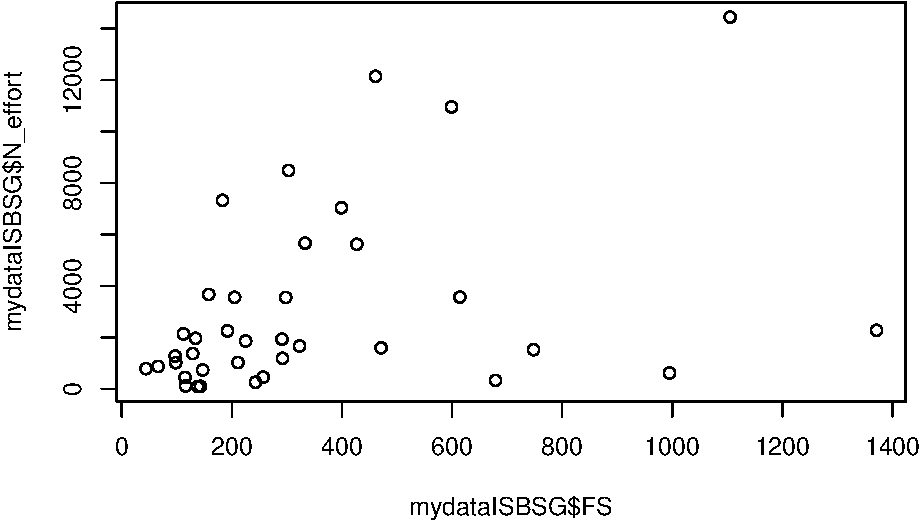
\includegraphics{DASE_files/figure-latex/plotExample-1.pdf}
\caption{\label{fig:plotExample}Simple plot}
\end{figure}

\begin{center}\rule{0.5\linewidth}{\linethickness}\end{center}

\section{Flow of Control}\label{flow-of-control}

Ifelse:

\begin{Shaded}
\begin{Highlighting}[]
\KeywordTok{library}\NormalTok{(foreign)}
\NormalTok{kc1 <-}\StringTok{ }\KeywordTok{read.arff}\NormalTok{(}\StringTok{"datasets/defectPred/D1/KC1.arff"}\NormalTok{)}
\NormalTok{kc1$Defective <-}\StringTok{ }\KeywordTok{ifelse}\NormalTok{(kc1$Defective ==}\StringTok{ "Y"}\NormalTok{, }\DecValTok{1}\NormalTok{, }\DecValTok{0}\NormalTok{)}
\KeywordTok{head}\NormalTok{(kc1, }\DecValTok{1}\NormalTok{)}
\end{Highlighting}
\end{Shaded}

\begin{verbatim}
##   LOC_BLANK BRANCH_COUNT LOC_CODE_AND_COMMENT LOC_COMMENTS
## 1         0            1                    0            0
##   CYCLOMATIC_COMPLEXITY DESIGN_COMPLEXITY ESSENTIAL_COMPLEXITY
## 1                     1                 1                    1
##   LOC_EXECUTABLE HALSTEAD_CONTENT HALSTEAD_DIFFICULTY HALSTEAD_EFFORT
## 1              3            11.58                2.67           82.35
##   HALSTEAD_ERROR_EST HALSTEAD_LENGTH HALSTEAD_LEVEL HALSTEAD_PROG_TIME
## 1               0.01              11           0.38               4.57
##   HALSTEAD_VOLUME NUM_OPERANDS NUM_OPERATORS NUM_UNIQUE_OPERANDS
## 1           30.88            4             7                   3
##   NUM_UNIQUE_OPERATORS LOC_TOTAL Defective
## 1                    4         5         0
\end{verbatim}

\section{Rattle}\label{rattle}

There is graphical interface, Rattle, that allow us to perform some data
mining tasks \citep{Williams11}.

\begin{figure}[htbp]
\centering
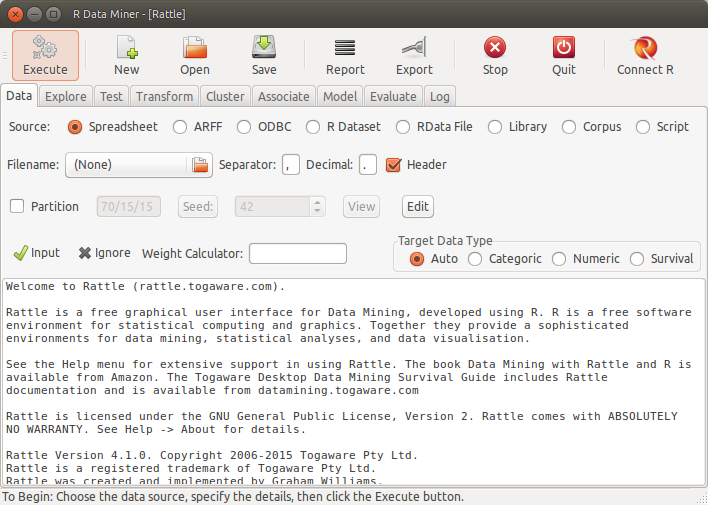
\includegraphics{./figures/rattle.png}
\caption{Rattle: GUI for Data mining with R}
\end{figure}

\part{Introduction to Data
Mining}\label{part-introduction-to-data-mining}

We will deal with extracting information from data, either for
estimation, defect prediction, planning, etc.

We will provide an overview of data analsyis using different techniques.

\chapter{What is Data Mining / Knowledge Discovery in Databases
(KDD)}\label{what-is-data-mining-knowledge-discovery-in-databases-kdd}

The non-trivial process of identifying valid, novel, potentially useful,
and ultimately understandable patterns in data \citep{FayyadPS1996}

\begin{figure}[htbp]
\centering
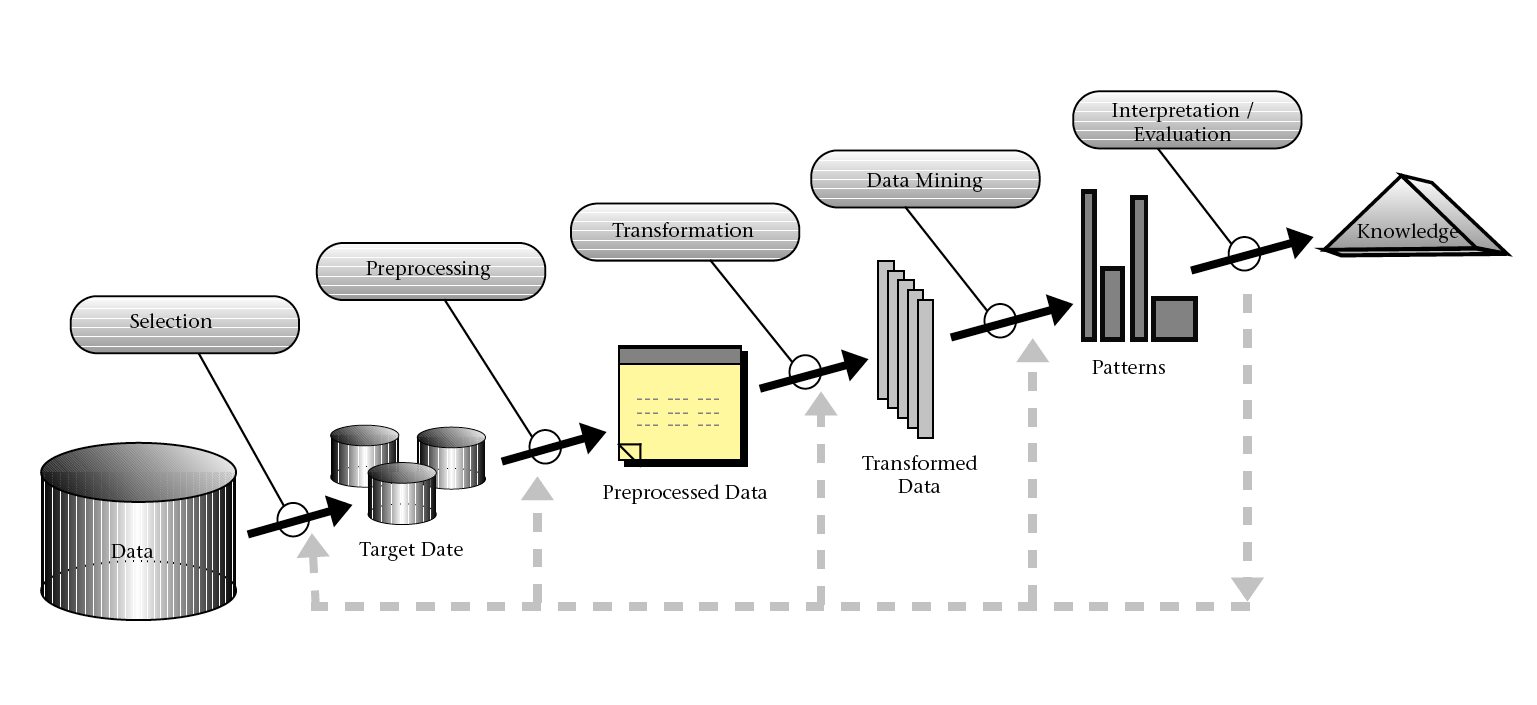
\includegraphics{figures/Fayyad96kdd-process.png}
\caption{KDD Process}
\end{figure}

The Cross Industry Process for Data Mining (CRISP-DM, 1996) also
provides a common and well-developed framework for delivering data
mining projects identifying six steps:

\begin{enumerate}
\def\labelenumi{\arabic{enumi}.}
\tightlist
\item
  Problem Understanding
\item
  Data Understanding
\item
  Data Preparation
\item
  Modeling
\item
  Evaluation
\item
  Deployment
\end{enumerate}

\section{The Aim of Data Analysis and Statistical
Learning}\label{the-aim-of-data-analysis-and-statistical-learning}

\begin{itemize}
\tightlist
\item
  The aim of any data analysis is to \textbf{understand the data}
\item
  and to build models for making predictions and estimating future
  events based on past data
\item
  and to make statistical inferences from our data.
\item
  We may want to test different hypothesis on the data
\item
  We want to generate conclusions about the population where our sample
  data comes from
\item
  Most probably we are interested in building a model for quality, time,
  defects or effort prediction
\end{itemize}

\begin{figure}[htbp]
\centering
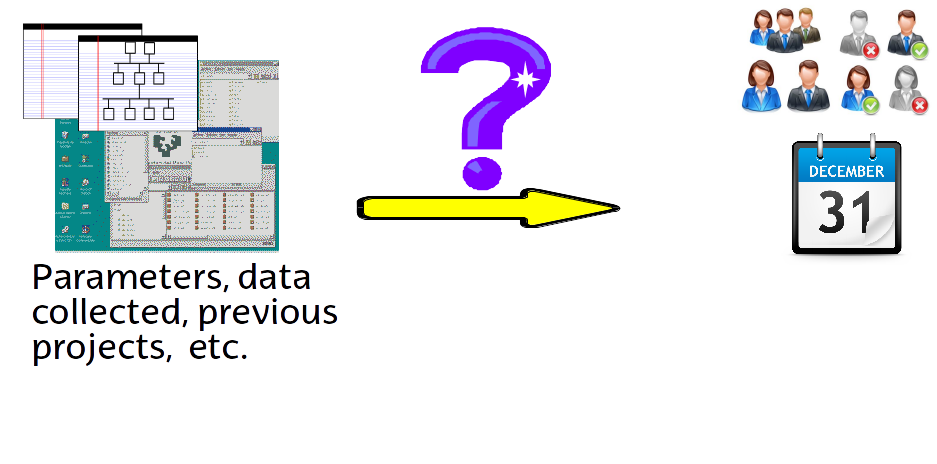
\includegraphics{figures/prediction.png}
\caption{}
\end{figure}

\begin{itemize}
\tightlist
\item
  We want to find a function \(f()\), that given \(X1, X2, ...\)
  computes \(Y=f(X1, X2, ..., Xn)\)
\end{itemize}

\section{Basic References}\label{basic-references}

Generic books about statistics:

\begin{itemize}
\item
  \href{https://cran.r-project.org/doc/contrib/Verzani-SimpleR.pdf}{John
  Verzani, \emph{simpleR - Using R for Introductory Statistics}}
\item
  \href{https://www.springer.com/gp/book/9780387790534}{Peter Dalgaard,
  \emph{Introductory Statistics with R}, 2nd Edt., Springer, 2008}
\item
  \href{http://www.springer.com/it/book/9781461471370}{Gareth James,
  Daniela Witten, Trevor Hastie, Robert Tibshirani, \emph{An
  Introduction to Statistical Learning with Applications in R},
  Springer, 2013}
\item
  \href{https://www.routledge.com/products/9780415879682}{Geoff Cumming,
  \emph{Understanding the New Statistics: Effect Sizes, Confidence
  Intervals, and Meta-Analysis}, Routledge, New York, 2012}
\end{itemize}

\section{Data Mining with R}\label{data-mining-with-r}

\begin{itemize}
\item
  \href{http://www.springer.com/gp/book/9781441998897}{Graham Williams,
  \emph{Data Mining with Rattle and R: The Art of Excavating Data for
  Knowledge Discovery}, Springer 2011}

  Also the author maintains a Web site:
  \url{http://rattle.togaware.com/}
\item
  \href{https://www.crcpress.com/Data-Mining-with-R-Learning-with-Case-Studies/Torgo/9781439810187}{Luis
  Torgo, \emph{Data Mining with R: Learning with Case Studies}, Chapman
  and Hall/CRC, 2010}
\item
  \url{http://www.rdatamining.com/}
\end{itemize}

\section{Data Mining with Weka}\label{data-mining-with-weka}

Weka is another popular framework in Java:

\begin{itemize}
\tightlist
\item
  Ian Witten, Eibe Frank, Mark Hall, Christopher J. Pal, Data Mining:
  Practical Machine Learning Tools and Techniques (4th Edt), Morgan
  Kaufmann, 2016, ISBN: 978-0128042915
\end{itemize}

\chapter{Data Sources in Software
Engineering}\label{data-sources-in-software-engineering}

We classify this trail in the following categories:

\begin{itemize}
\item
  \emph{Source code} can be studied to measure its properties, such as
  size or complexity.
\item
  \emph{Source Code Management Systems} (SCM) make it possible to store
  all the changes that the different source code files undergo during
  the project. Also, SCM systems allow for work to be done in parallel
  by different developers over the same source code tree. Every change
  recorded in the system is accompanied with meta-information (author,
  date, reason for the change, etc) that can be used for research
  purposes.
\item
  \emph{Issue or Bug tracking systems} (ITS). Bugs, defects and user
  requests are managed in ISTs, where users and developers can fill
  tickets with a description of a defect found, or a desired new
  functionality. All the changes to the ticket are recorded in the
  system, and most of the systems also record the comments and
  communications among all the users and developers implied in the task.
\item
  \emph{Messages} between developers and users. In the case of free/open
  source software, the projects are open to the world, and the messages
  are archived in the form of mailing lists and social networks which
  can also be mined for research purposes. There are also some other
  open message systems, such as IRC or forums.
\item
  \emph{Meta-data about the projects}. As well as the low level
  information of the software processes, we can also find meta-data
  about the software projects which can be useful for research. This
  meta-data may include intended-audience, programming language, domain
  of application, license (in the case of open source), etc.
\item
  \emph{Usage data}. There are statistics about software downloads, logs
  from servers, software reviews, etc.
\end{itemize}

\section{Types of information stored in the
repositories}\label{types-of-information-stored-in-the-repositories}

\begin{itemize}
\item
  Meta-information about the project itself and the people that
  participated.

  \begin{itemize}
  \item
    Low-level information

    \begin{itemize}
    \item
      Mailing Lists (ML)
    \item
      Bugs Tracking Systems (BTS) or Project Tracker System (PTS)
    \item
      Software Configuration Management Systems (SCM)
    \end{itemize}
  \item
    Processed information. For example project management information
    about the effort estimation and cost of the project.
  \end{itemize}
\item
  Whether the repository is public or not
\item
  Single project vs.~multiprojects. Whether the repository contains
  information of a single project with multiples versions or multiples
  projects and/or versions.
\item
  Type of content, open source or industrial projects
\item
  Format in which the information is stored and formats or technologies
  for accessing the information:

  \begin{itemize}
  \item
    Text. It can be just plain text, CSV (Comma Separated Values) files,
    Attribute-Relation File Format (ARFF) or its variants
  \item
    Through databases. Downloading dumps of the database.
  \item
    Remote access such as APIs of Web services or REST
  \end{itemize}
\end{itemize}

\section{Repositories}\label{repositories}

There is a number of open research repositories in Software Engineering.
Among them:

\begin{itemize}
\item
  FLOSSMole \citep{HCC06} \url{http://flossmole.org/}
\item
  FLOSSMetrics \citep{herraiz2009flossmetrics}:
  \url{http://flossmetrics.org/}
\item
  PROMISE (PRedictOr Models In Software Engineering) {[}8{]}:
  \url{http://openscience.us/repo/}
\item
  Qualitas Corpus (QC) \citep{QualitasCorpus2010}:
  \url{http://qualitascorpus.com/}
\item
  Sourcerer Project \citep{LBNRB09}: \url{http://sourcerer.ics.uci.edu/}
\item
  Ultimate Debian Database (UDD) \citep{NZ10}
  \url{http://udd.debian.org/}
\item
  SourceForge Research Data Archive (SRDA) \citep{VanAntwerpM2008}
  \url{http://zerlot.cse.nd.edu/}
\item
  SECOLD (Source code ECOsystem Linked Data):
  \url{http://www.secold.org/}
\item
  Software-artifact Infrastructure Repository (SIR)
  {[}\url{http://sir.unl.edu}{]}
\item
  OpenHub: \url{https://www.openhub.net/}
\end{itemize}

Not openly available:

\begin{itemize}
\item
  The International Software Benchmarking Standards Group (ISBSG)
  \url{http://www.isbsg.org/}
\item
  TukuTuku \url{http://www.metriq.biz/tukutuku/}
\end{itemize}

Some papers and publications/theses that have been used in the
literature:

\begin{itemize}
\item
  Helix Data Set \citep{Vasa2010}:
  \url{http://www.ict.swin.edu.au/research/projects/helix/}
\item
  Bug Prediction Dataset (BPD) \citep[\citet{ALR11}]{DAmb2010a}:
  \url{http://bug.inf.usi.ch/}
\item
  Eclipse Bug Data (EBD) \citep[\citet{NZZH12}]{ZPZ07}:
  \url{http://www.st.cs.uni-saarland.de/softevo/bug-data/eclipse/}
\end{itemize}

\section{Some Tools/Dashboards to extract
data}\label{some-toolsdashboards-to-extract-data}

Within the open source community, two toolkits allow us to extract data
that can be used to explore projects:

Metrics Grimoire \url{http://metricsgrimoire.github.io/}

SonarQube \url{http://www.sonarqube.org/}

\section{Effort Estimation Data in Software
Engineering}\label{effort-estimation-data-in-software-engineering}

It is worth highlighting the case of software effort estimation datasets
with their peculiarities. First, most effort estimation datasets used in
the literature are scattered through research papers with the exception
of a few kept in the PROMISE repository. Mair et al
\citeyearpar{MairSJ05} also have analysed available datasets in the
field of cost estimation identifying 65 different datasets in 50 papers.

Second, their size is very small with the exception of ISBSG repository
discussed previously which a small sample is available through PROMISE
and the China dataset with 499 instances.

Third, some can be quite old in a context and time that is not
applicable to current development environments. The authors noted that
the oldest datasets (COCOMO, Desharnais, Kemerer and Albrecht and
Gaffney) tend to be the most studied ones and a subset of the most
relevant ones. Also, from the artificial intelligence or data mining
point of view effort estimation has been mainly tackled with different
types of regression techniques and more recently with techniques which
are also typically considered under the umbrella of data mining
techniques. However, as the number of examples per dataset is
increasing, other machine learning techniques are also being studied
(e.g.: Dejaeger et al \citeyearpar{Dejaeger_TSE12_EffEst} report on a
comparison of several machine learning techniques to effort estimation
with only 5 out the 9 used datasets publicly available). From the data
mining point of view, the small number of instances hinders the
application of machine learning techniques.

However, software effort and cost estimation still remain one of the
main challenges in software engineering and have attracted a great deal
of interest by many researchers \citeyearpar{Jorgensen07}. For example,
there are continuous analyses of whether software development follows
economies or diseconomies of scale (see
\citep[\citet{Banker1994},\citet{Kitchenham2002}]{Dolado01_CostEst}).

Next Table \ref{tab:effEstimation} (following Mair et al
\citeyearpar{MairSJ05} ) shows the most open cost/effort datasets
available in the literature with their main reference.

\begin{longtable}[]{@{}lrr@{}}
\caption{\label{tab:effEstimation} Effort Estimation Dataset from
articles}\tabularnewline
\toprule
\begin{minipage}[b]{0.44\columnwidth}\raggedright\strut
Reference\strut
\end{minipage} & \begin{minipage}[b]{0.18\columnwidth}\raggedleft\strut
Instances\strut
\end{minipage} & \begin{minipage}[b]{0.18\columnwidth}\raggedleft\strut
Attributes\strut
\end{minipage}\tabularnewline
\midrule
\endfirsthead
\toprule
\begin{minipage}[b]{0.44\columnwidth}\raggedright\strut
Reference\strut
\end{minipage} & \begin{minipage}[b]{0.18\columnwidth}\raggedleft\strut
Instances\strut
\end{minipage} & \begin{minipage}[b]{0.18\columnwidth}\raggedleft\strut
Attributes\strut
\end{minipage}\tabularnewline
\midrule
\endhead
\begin{minipage}[t]{0.44\columnwidth}\raggedright\strut
Abran and Robillard \citeyearpar{Abran_TSE96_FP}\strut
\end{minipage} & \begin{minipage}[t]{0.18\columnwidth}\raggedleft\strut
21\strut
\end{minipage} & \begin{minipage}[t]{0.18\columnwidth}\raggedleft\strut
31\strut
\end{minipage}\tabularnewline
\begin{minipage}[t]{0.44\columnwidth}\raggedright\strut
Albrecht-Gaffney \citeyearpar{AlbrechtG83}\strut
\end{minipage} & \begin{minipage}[t]{0.18\columnwidth}\raggedleft\strut
24\strut
\end{minipage} & \begin{minipage}[t]{0.18\columnwidth}\raggedleft\strut
7\strut
\end{minipage}\tabularnewline
\begin{minipage}[t]{0.44\columnwidth}\raggedright\strut
Bailey and Basili \citeyearpar{Bailey81}\strut
\end{minipage} & \begin{minipage}[t]{0.18\columnwidth}\raggedleft\strut
18\strut
\end{minipage} & \begin{minipage}[t]{0.18\columnwidth}\raggedleft\strut
9\strut
\end{minipage}\tabularnewline
\begin{minipage}[t]{0.44\columnwidth}\raggedright\strut
Belady and Lehman \citeyearpar{Belady79}\strut
\end{minipage} & \begin{minipage}[t]{0.18\columnwidth}\raggedleft\strut
33\strut
\end{minipage} & \begin{minipage}[t]{0.18\columnwidth}\raggedleft\strut
\strut
\end{minipage}\tabularnewline
\begin{minipage}[t]{0.44\columnwidth}\raggedright\strut
Boehm (aka COCOMO Dataset) \citeyearpar{Boehm81}\strut
\end{minipage} & \begin{minipage}[t]{0.18\columnwidth}\raggedleft\strut
63\strut
\end{minipage} & \begin{minipage}[t]{0.18\columnwidth}\raggedleft\strut
43\strut
\end{minipage}\tabularnewline
\begin{minipage}[t]{0.44\columnwidth}\raggedright\strut
Desharnais \citeyearpar{Desharnais88}\strut
\end{minipage} & \begin{minipage}[t]{0.18\columnwidth}\raggedleft\strut
61\strut
\end{minipage} & \begin{minipage}[t]{0.18\columnwidth}\raggedleft\strut
10\strut
\end{minipage}\tabularnewline
\begin{minipage}[t]{0.44\columnwidth}\raggedright\strut
Dolado \citeyearpar{Dolado97}\strut
\end{minipage} & \begin{minipage}[t]{0.18\columnwidth}\raggedleft\strut
24\strut
\end{minipage} & \begin{minipage}[t]{0.18\columnwidth}\raggedleft\strut
7\strut
\end{minipage}\tabularnewline
\begin{minipage}[t]{0.44\columnwidth}\raggedright\strut
Hastings and Sajeev \citeyearpar{Hastings01}\strut
\end{minipage} & \begin{minipage}[t]{0.18\columnwidth}\raggedleft\strut
8\strut
\end{minipage} & \begin{minipage}[t]{0.18\columnwidth}\raggedleft\strut
14\strut
\end{minipage}\tabularnewline
\begin{minipage}[t]{0.44\columnwidth}\raggedright\strut
Heiat and Heiat \citep{Heiat97}\strut
\end{minipage} & \begin{minipage}[t]{0.18\columnwidth}\raggedleft\strut
35\strut
\end{minipage} & \begin{minipage}[t]{0.18\columnwidth}\raggedleft\strut
4\strut
\end{minipage}\tabularnewline
\begin{minipage}[t]{0.44\columnwidth}\raggedright\strut
Jeffery and Stathis \citeyearpar{Jeffery_ESE96}\strut
\end{minipage} & \begin{minipage}[t]{0.18\columnwidth}\raggedleft\strut
17\strut
\end{minipage} & \begin{minipage}[t]{0.18\columnwidth}\raggedleft\strut
7\strut
\end{minipage}\tabularnewline
\begin{minipage}[t]{0.44\columnwidth}\raggedright\strut
Jorgensen \citeyearpar{Jorgensen04}\strut
\end{minipage} & \begin{minipage}[t]{0.18\columnwidth}\raggedleft\strut
47\strut
\end{minipage} & \begin{minipage}[t]{0.18\columnwidth}\raggedleft\strut
4\strut
\end{minipage}\tabularnewline
\begin{minipage}[t]{0.44\columnwidth}\raggedright\strut
Jorgensen et al. \citeyearpar{Jorgensen2003}\strut
\end{minipage} & \begin{minipage}[t]{0.18\columnwidth}\raggedleft\strut
20\strut
\end{minipage} & \begin{minipage}[t]{0.18\columnwidth}\raggedleft\strut
4\strut
\end{minipage}\tabularnewline
\begin{minipage}[t]{0.44\columnwidth}\raggedright\strut
Kemerer \citeyearpar{Kemerer87}\strut
\end{minipage} & \begin{minipage}[t]{0.18\columnwidth}\raggedleft\strut
15\strut
\end{minipage} & \begin{minipage}[t]{0.18\columnwidth}\raggedleft\strut
5\strut
\end{minipage}\tabularnewline
\begin{minipage}[t]{0.44\columnwidth}\raggedright\strut
Kitchenham (Mermaid 2) \citeyearpar{Kitchenham2002}\strut
\end{minipage} & \begin{minipage}[t]{0.18\columnwidth}\raggedleft\strut
30\strut
\end{minipage} & \begin{minipage}[t]{0.18\columnwidth}\raggedleft\strut
5\strut
\end{minipage}\tabularnewline
\begin{minipage}[t]{0.44\columnwidth}\raggedright\strut
Kitchenham et al. (CSC) \citeyearpar{Kitchenham02_CSC}\strut
\end{minipage} & \begin{minipage}[t]{0.18\columnwidth}\raggedleft\strut
145\strut
\end{minipage} & \begin{minipage}[t]{0.18\columnwidth}\raggedleft\strut
9\strut
\end{minipage}\tabularnewline
\begin{minipage}[t]{0.44\columnwidth}\raggedright\strut
Kitchenham and Taylor (ICL) \citeyearpar{Kitchenham85}\strut
\end{minipage} & \begin{minipage}[t]{0.18\columnwidth}\raggedleft\strut
10\strut
\end{minipage} & \begin{minipage}[t]{0.18\columnwidth}\raggedleft\strut
6\strut
\end{minipage}\tabularnewline
\begin{minipage}[t]{0.44\columnwidth}\raggedright\strut
Kitchenham and Taylor (BT System X) \citeyearpar{Kitchenham85}\strut
\end{minipage} & \begin{minipage}[t]{0.18\columnwidth}\raggedleft\strut
10\strut
\end{minipage} & \begin{minipage}[t]{0.18\columnwidth}\raggedleft\strut
3\strut
\end{minipage}\tabularnewline
\begin{minipage}[t]{0.44\columnwidth}\raggedright\strut
Kitchenham and Taylor (BT Software Houses)
\citeyearpar{Kitchenham85}\strut
\end{minipage} & \begin{minipage}[t]{0.18\columnwidth}\raggedleft\strut
12\strut
\end{minipage} & \begin{minipage}[t]{0.18\columnwidth}\raggedleft\strut
6\strut
\end{minipage}\tabularnewline
\begin{minipage}[t]{0.44\columnwidth}\raggedright\strut
Keung et al. (China dataset) \citeyearpar{Keung11}\footnotemark{}\strut
\end{minipage}
\footnotetext{Donated through PROMISE.} &
\begin{minipage}[t]{0.18\columnwidth}\raggedleft\strut
499\strut
\end{minipage} & \begin{minipage}[t]{0.18\columnwidth}\raggedleft\strut
18\strut
\end{minipage}\tabularnewline
\begin{minipage}[t]{0.44\columnwidth}\raggedright\strut
Li et al.(USP05) \citeyearpar{LiRAR07}\footnotemark{}\strut
\end{minipage}
\footnotetext{Only a subset of the data in the paper, the complete
  dataset is donated through PROMISE} &
\begin{minipage}[t]{0.18\columnwidth}\raggedleft\strut
202\strut
\end{minipage} & \begin{minipage}[t]{0.18\columnwidth}\raggedleft\strut
16\strut
\end{minipage}\tabularnewline
\begin{minipage}[t]{0.44\columnwidth}\raggedright\strut
Mišić and Tevsić \citeyearpar{Misic19981}\strut
\end{minipage} & \begin{minipage}[t]{0.18\columnwidth}\raggedleft\strut
6\strut
\end{minipage} & \begin{minipage}[t]{0.18\columnwidth}\raggedleft\strut
16\strut
\end{minipage}\tabularnewline
\begin{minipage}[t]{0.44\columnwidth}\raggedright\strut
Maxwell (Dev Effort) \citeyearpar{Maxwell02}\strut
\end{minipage} & \begin{minipage}[t]{0.18\columnwidth}\raggedleft\strut
63\strut
\end{minipage} & \begin{minipage}[t]{0.18\columnwidth}\raggedleft\strut
32\strut
\end{minipage}\tabularnewline
\begin{minipage}[t]{0.44\columnwidth}\raggedright\strut
Maxwell (Maintenance Eff) \citeyearpar{Maxwell02}\strut
\end{minipage} & \begin{minipage}[t]{0.18\columnwidth}\raggedleft\strut
67\strut
\end{minipage} & \begin{minipage}[t]{0.18\columnwidth}\raggedleft\strut
28\strut
\end{minipage}\tabularnewline
\begin{minipage}[t]{0.44\columnwidth}\raggedright\strut
Miyazaki et al. \citeyearpar{Miyazaki94}\strut
\end{minipage} & \begin{minipage}[t]{0.18\columnwidth}\raggedleft\strut
47\strut
\end{minipage} & \begin{minipage}[t]{0.18\columnwidth}\raggedleft\strut
9\strut
\end{minipage}\tabularnewline
\begin{minipage}[t]{0.44\columnwidth}\raggedright\strut
Moser et al. \citeyearpar{Moser1999}\strut
\end{minipage} & \begin{minipage}[t]{0.18\columnwidth}\raggedleft\strut
37\strut
\end{minipage} & \begin{minipage}[t]{0.18\columnwidth}\raggedleft\strut
4\strut
\end{minipage}\tabularnewline
\begin{minipage}[t]{0.44\columnwidth}\raggedright\strut
Shepperd and Cartwright \citep{Shepperd_TSE01}\strut
\end{minipage} & \begin{minipage}[t]{0.18\columnwidth}\raggedleft\strut
39\strut
\end{minipage} & \begin{minipage}[t]{0.18\columnwidth}\raggedleft\strut
3\strut
\end{minipage}\tabularnewline
\begin{minipage}[t]{0.44\columnwidth}\raggedright\strut
Shepperd and Schofield (Telecom 1)
\citeyearpar{Shepperd97_Analogy}\strut
\end{minipage} & \begin{minipage}[t]{0.18\columnwidth}\raggedleft\strut
18\strut
\end{minipage} & \begin{minipage}[t]{0.18\columnwidth}\raggedleft\strut
5\strut
\end{minipage}\tabularnewline
\begin{minipage}[t]{0.44\columnwidth}\raggedright\strut
Schofield (real-time 1)
\citeyearpar[\citet{Shepperd97_Analogy}]{Schofield98PhD}\strut
\end{minipage} & \begin{minipage}[t]{0.18\columnwidth}\raggedleft\strut
21\strut
\end{minipage} & \begin{minipage}[t]{0.18\columnwidth}\raggedleft\strut
4\strut
\end{minipage}\tabularnewline
\begin{minipage}[t]{0.44\columnwidth}\raggedright\strut
Schofield (Mermaid) \citeyearpar{Schofield98PhD}\strut
\end{minipage} & \begin{minipage}[t]{0.18\columnwidth}\raggedleft\strut
30\strut
\end{minipage} & \begin{minipage}[t]{0.18\columnwidth}\raggedleft\strut
18\strut
\end{minipage}\tabularnewline
\begin{minipage}[t]{0.44\columnwidth}\raggedright\strut
Schofield (Finnish) \citeyearpar{Schofield98PhD}\strut
\end{minipage} & \begin{minipage}[t]{0.18\columnwidth}\raggedleft\strut
39\strut
\end{minipage} & \begin{minipage}[t]{0.18\columnwidth}\raggedleft\strut
30\strut
\end{minipage}\tabularnewline
\begin{minipage}[t]{0.44\columnwidth}\raggedright\strut
Schofield (Hughes) \citeyearpar{Schofield98PhD}\strut
\end{minipage} & \begin{minipage}[t]{0.18\columnwidth}\raggedleft\strut
33\strut
\end{minipage} & \begin{minipage}[t]{0.18\columnwidth}\raggedleft\strut
14\strut
\end{minipage}\tabularnewline
\begin{minipage}[t]{0.44\columnwidth}\raggedright\strut
Woodfield et al. \citeyearpar{Woodfield81}\strut
\end{minipage} & \begin{minipage}[t]{0.18\columnwidth}\raggedleft\strut
63\strut
\end{minipage} & \begin{minipage}[t]{0.18\columnwidth}\raggedleft\strut
8\strut
\end{minipage}\tabularnewline
\bottomrule
\end{longtable}

\part{Exploratory and Descriptive Data
analysis}\label{part-exploratory-and-descriptive-data-analysis}

\chapter{Exploratory Data Analysis}\label{exploratory-data-analysis}

\section{Descriptive statistics}\label{descriptive-statistics}

\emph{The first task with any dataset is to characterise it in terms of
summary statistics and graphics } Displaying information graphically
will help us to identify the main characteristics of the data. To
describe a distribution we often want to know where it is centered and
and what the spread is (mean, median, quantiles)

\section{Basic Plots}\label{basic-plots}

\begin{verbatim}
* _Histogram_ defines a sequence of breaks and then counts the number of observations in the bins formed by the breaks.

* **Boxplot** used to summarize data succinctly, quickly displaying if the data is symmetric or has suspected outliers.  
![Boxplot description](./figures/boxplotexp.png)
  
  
* _Q-Q plot_ is used to determine if the data is close to being normally distributed. The quantiles of the standard normal distribution is represented by a straight line. The normality of the data can be evaluated by observing the extent in which the points appear on the line. When the data is normally distributed around the mean, then the mean and the median should be equal. 

* _Scatterplot_ provides a graphical view of the relationship between two sets of numbers: one numerical variable against another. 

* _Kernel Density_ plot_ visualizes the underlying distribution of a variable. Kernel density estimatiion is a non-parametric method of estimating the probability density function of continuous random variable. It helps to identify the distribution of the variable.

* _Violin Plot_ is a combination of a boxplot and a kernel density plot. 
\end{verbatim}

\section{Normality}\label{normality}

\begin{itemize}
\tightlist
\item
  A normal distribution is an arrangement of a data set in which most
  values cluster in the middle of the range
\item
  A graphical representation of a normal distribution is sometimes
  called a \emph{bell curve} because of its shape.
\item
  Many procedures in statistics are based on this property.
  \emph{Parametric} procedures require the normality property.
\item
  In a normal distribution about 95\% of the probability lies within 2
  Standard Deviations of the mean.
\item
  Two examples: one population with mean 60 and the standard deviation
  of 1, and the other with mean 60 and \(sd=4\) (means shifted to 0)
\end{itemize}

\begin{Shaded}
\begin{Highlighting}[]
\NormalTok{main.title <-}\StringTok{ "Area within 2SD of the mean"}
\KeywordTok{par}\NormalTok{(}\DataTypeTok{mfrow=}\KeywordTok{c}\NormalTok{(}\DecValTok{1}\NormalTok{,}\DecValTok{2}\NormalTok{))}
\KeywordTok{plot}\NormalTok{(function(x) }\KeywordTok{dnorm}\NormalTok{(x, }\DataTypeTok{mean =} \DecValTok{0}\NormalTok{, }\DataTypeTok{sd =} \DecValTok{1}\NormalTok{),}
\DataTypeTok{xlim =} \KeywordTok{c}\NormalTok{(-}\DecValTok{3}\NormalTok{, }\DecValTok{3}\NormalTok{), }\DataTypeTok{main =} \StringTok{"SD 1"}\NormalTok{, }\DataTypeTok{xlab =} \StringTok{"x"}\NormalTok{,}
\DataTypeTok{ylab =} \StringTok{""}\NormalTok{, }\DataTypeTok{cex =} \DecValTok{2}\NormalTok{)}
\KeywordTok{segments}\NormalTok{(-}\DecValTok{2}\NormalTok{, }\DecValTok{0}\NormalTok{, -}\DecValTok{2}\NormalTok{, }\FloatTok{0.4}\NormalTok{)}
\KeywordTok{segments}\NormalTok{(}\DecValTok{2}\NormalTok{, }\DecValTok{0}\NormalTok{, }\DecValTok{2}\NormalTok{, }\FloatTok{0.4}\NormalTok{)}
\KeywordTok{plot}\NormalTok{(function(x) }\KeywordTok{dnorm}\NormalTok{(x, }\DataTypeTok{mean =} \DecValTok{0}\NormalTok{, }\DataTypeTok{sd =} \DecValTok{4}\NormalTok{),}
\DataTypeTok{xlim =} \KeywordTok{c}\NormalTok{(-}\DecValTok{12}\NormalTok{, }\DecValTok{12}\NormalTok{), }\DataTypeTok{main =} \StringTok{"SD 4"}\NormalTok{, }\DataTypeTok{xlab =} \StringTok{"x"}\NormalTok{,}
\DataTypeTok{ylab =} \StringTok{""}\NormalTok{, }\DataTypeTok{cex =} \DecValTok{2}\NormalTok{)}
\KeywordTok{segments}\NormalTok{(-}\DecValTok{8}\NormalTok{, }\DecValTok{0}\NormalTok{, -}\DecValTok{8}\NormalTok{, }\FloatTok{0.1}\NormalTok{)}
\KeywordTok{segments}\NormalTok{(}\DecValTok{8}\NormalTok{, }\DecValTok{0}\NormalTok{, }\DecValTok{8}\NormalTok{, }\FloatTok{0.1}\NormalTok{)}
\end{Highlighting}
\end{Shaded}

\begin{figure}[htbp]
\centering
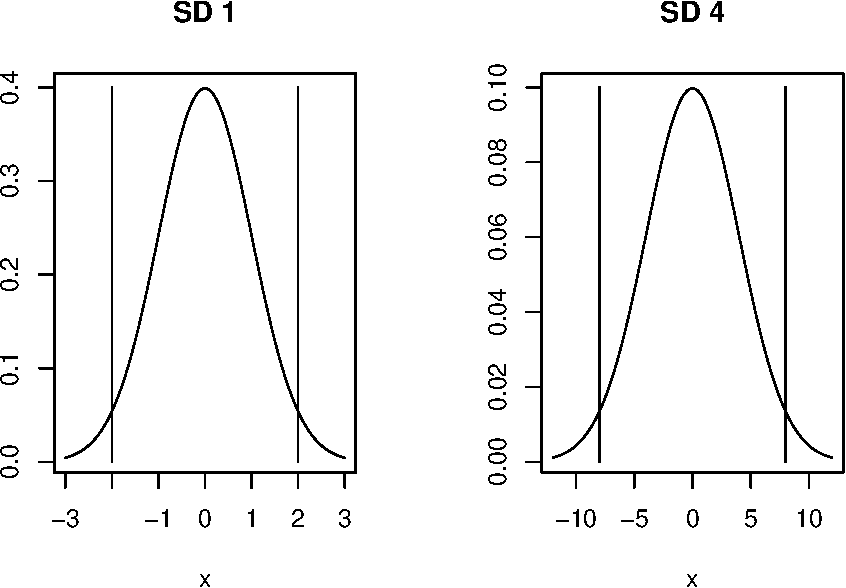
\includegraphics{DASE_files/figure-latex/SDPlotExample-1.pdf}
\caption{\label{fig:SDPlotExample}Plot exaple of the area within 2 SD of the
mean}
\end{figure}

\begin{itemize}
\tightlist
\item
  if we sample from this population we get ``another
  population''.fig.cap=``Simple plot''
\end{itemize}

\begin{Shaded}
\begin{Highlighting}[]
\NormalTok{sample.means <-}\StringTok{ }\KeywordTok{rep}\NormalTok{(}\OtherTok{NA}\NormalTok{, }\DecValTok{1000}\NormalTok{)}
\NormalTok{for (i in }\DecValTok{1}\NormalTok{:}\DecValTok{1000}\NormalTok{) \{}
  \NormalTok{sample}\FloatTok{.40} \NormalTok{<-}\StringTok{ }\KeywordTok{rnorm}\NormalTok{(}\DecValTok{40}\NormalTok{, }\DataTypeTok{mean =} \DecValTok{60}\NormalTok{, }\DataTypeTok{sd =} \DecValTok{4}\NormalTok{) }\CommentTok{#rnorm generates random numbers from normal distribution}
  \NormalTok{sample.means[i] <-}\StringTok{ }\KeywordTok{mean}\NormalTok{(sample}\FloatTok{.40}\NormalTok{)}
\NormalTok{\}}
\NormalTok{means40 <-}\StringTok{ }\KeywordTok{mean}\NormalTok{(sample.means)}
\NormalTok{sd40 <-}\StringTok{ }\KeywordTok{sd}\NormalTok{(sample.means)}
\NormalTok{means40}
\end{Highlighting}
\end{Shaded}

\begin{verbatim}
## [1] 60.00314
\end{verbatim}

\begin{Shaded}
\begin{Highlighting}[]
\NormalTok{sd40}
\end{Highlighting}
\end{Shaded}

\begin{verbatim}
## [1] 0.6225441
\end{verbatim}

\begin{itemize}
\tightlist
\item
  These sample means are another ``population''. The sampling
  distribution of the sample mean is normally distributed meaning that
  the ``mean of a representative sample provides an estimate of the
  unknown population mean''. This is shown in Figure
  \ref{fig:sampleMeansExample}
\end{itemize}

\begin{Shaded}
\begin{Highlighting}[]
\KeywordTok{hist}\NormalTok{(sample.means)}
\end{Highlighting}
\end{Shaded}

\begin{figure}[htbp]
\centering
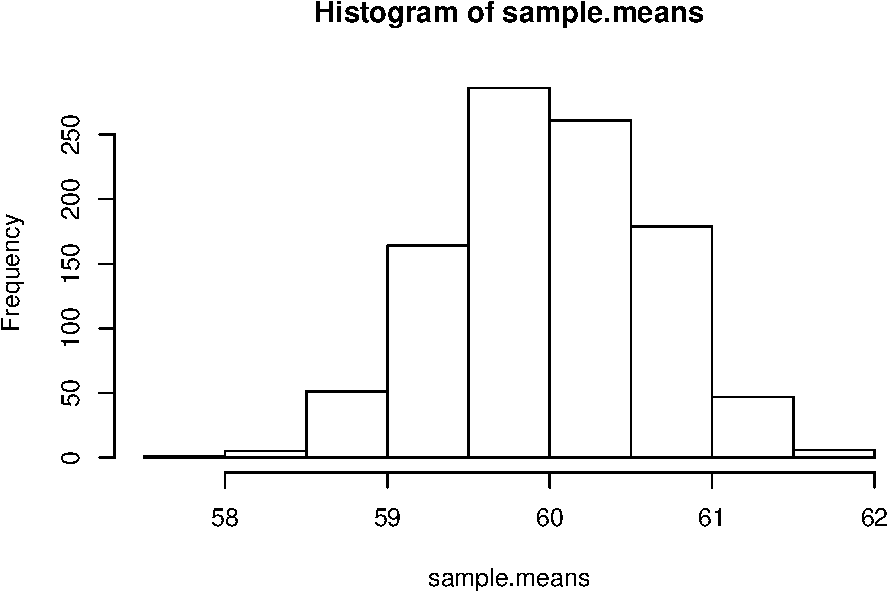
\includegraphics{DASE_files/figure-latex/sampleMeansExample-1.pdf}
\caption{\label{fig:sampleMeansExample}Sample means histogram}
\end{figure}

\section{Running Example}\label{running-example}

\begin{itemize}
\tightlist
\item
  Set the path to your files
\item
  Read the \emph{Telecom1} dataset and print out the summary statistics
  with the command \texttt{summary}
\end{itemize}

\begin{Shaded}
\begin{Highlighting}[]
\KeywordTok{options}\NormalTok{(}\DataTypeTok{digits=}\DecValTok{3}\NormalTok{)}
\NormalTok{telecom1 <-}\StringTok{ }\KeywordTok{read.table}\NormalTok{(}\StringTok{"./datasets/effortEstimation/Telecom1.csv"}\NormalTok{, }\DataTypeTok{sep=}\StringTok{","}\NormalTok{,}\DataTypeTok{header=}\OtherTok{TRUE}\NormalTok{, }\DataTypeTok{stringsAsFactors=}\OtherTok{FALSE}\NormalTok{, }\DataTypeTok{dec =} \StringTok{"."}\NormalTok{) }\CommentTok{#read data}
\KeywordTok{summary}\NormalTok{(telecom1)}
\end{Highlighting}
\end{Shaded}

\begin{verbatim}
##       size           effort        EstTotal  
##  Min.   :  3.0   Min.   :  24   Min.   : 30  
##  1st Qu.: 37.2   1st Qu.: 119   1st Qu.:142  
##  Median : 68.5   Median : 222   Median :289  
##  Mean   :100.3   Mean   : 284   Mean   :320  
##  3rd Qu.:164.0   3rd Qu.: 352   3rd Qu.:472  
##  Max.   :284.0   Max.   :1116   Max.   :777
\end{verbatim}

\begin{itemize}
\tightlist
\item
  We see that this dataset has three variables (or parameters) and few
  data points (18)

  \begin{itemize}
  \tightlist
  \item
    size: the independent variable
  \item
    effort: the dependent variable
  \item
    EstTotal: the estimates coming from an estimation method
  \end{itemize}
\item
  Basic Plots
\end{itemize}

\begin{Shaded}
\begin{Highlighting}[]
\KeywordTok{par}\NormalTok{(}\DataTypeTok{mfrow=}\KeywordTok{c}\NormalTok{(}\DecValTok{1}\NormalTok{,}\DecValTok{2}\NormalTok{)) }\CommentTok{#n figures per row}
\NormalTok{size_telecom1 <-}\StringTok{ }\NormalTok{telecom1$size}
\NormalTok{effort_telecom1 <-}\StringTok{ }\NormalTok{telecom1$effort}

\KeywordTok{hist}\NormalTok{(size_telecom1, }\DataTypeTok{col=}\StringTok{"blue"}\NormalTok{, }\DataTypeTok{xlab=}\StringTok{'size'}\NormalTok{, }\DataTypeTok{ylab =} \StringTok{'Probability'}\NormalTok{, }\DataTypeTok{main =} \StringTok{'Histogram of project Size'}\NormalTok{)}
\KeywordTok{lines}\NormalTok{(}\KeywordTok{density}\NormalTok{(size_telecom1, }\DataTypeTok{na.rm =} \NormalTok{T, }\DataTypeTok{from =} \DecValTok{0}\NormalTok{, }\DataTypeTok{to =} \KeywordTok{max}\NormalTok{(size_telecom1)))}
\KeywordTok{plot}\NormalTok{(}\KeywordTok{density}\NormalTok{(size_telecom1))}
\end{Highlighting}
\end{Shaded}

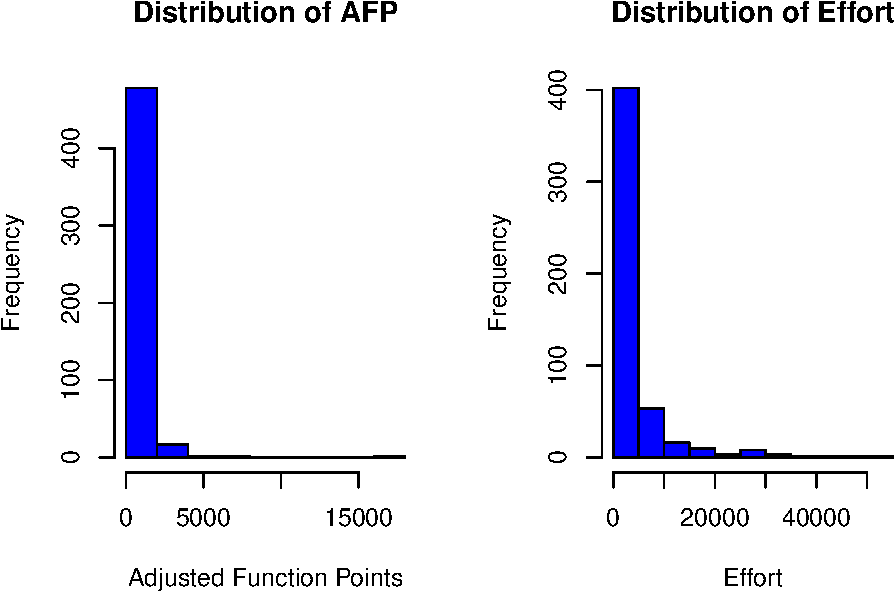
\includegraphics{DASE_files/figure-latex/unnamed-chunk-19-1.pdf}

\begin{Shaded}
\begin{Highlighting}[]
\KeywordTok{hist}\NormalTok{(effort_telecom1, }\DataTypeTok{col=}\StringTok{"blue"}\NormalTok{)}
\KeywordTok{plot}\NormalTok{(}\KeywordTok{density}\NormalTok{(effort_telecom1))}
\end{Highlighting}
\end{Shaded}

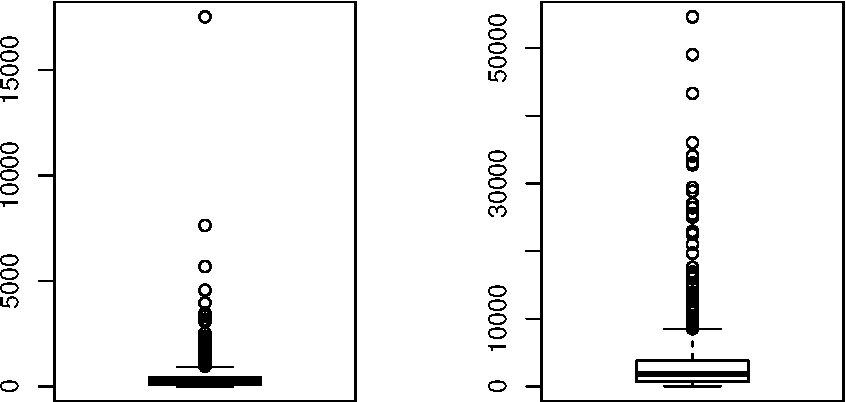
\includegraphics{DASE_files/figure-latex/unnamed-chunk-19-2.pdf}

\begin{Shaded}
\begin{Highlighting}[]
\KeywordTok{boxplot}\NormalTok{(size_telecom1)}
\KeywordTok{boxplot}\NormalTok{(effort_telecom1)}
\end{Highlighting}
\end{Shaded}

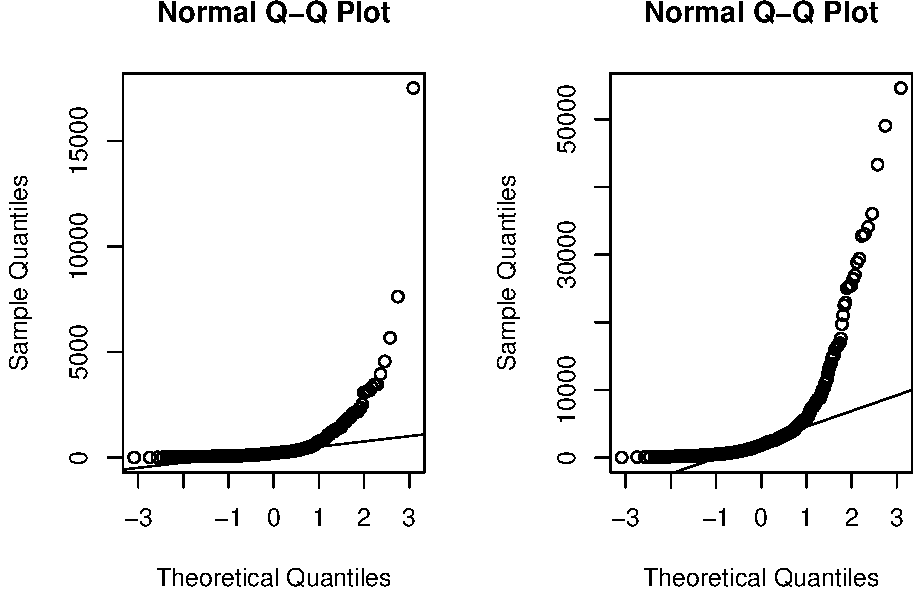
\includegraphics{DASE_files/figure-latex/unnamed-chunk-19-3.pdf}

\begin{Shaded}
\begin{Highlighting}[]
\CommentTok{# violin plots for those two variables}
\KeywordTok{library}\NormalTok{(vioplot)}
\KeywordTok{vioplot}\NormalTok{(size_telecom1, }\DataTypeTok{names =} \StringTok{''}\NormalTok{) }
\KeywordTok{title}\NormalTok{(}\StringTok{"Violin Plot of Project Size"}\NormalTok{)}
\KeywordTok{vioplot}\NormalTok{(effort_telecom1, }\DataTypeTok{names =} \StringTok{''}\NormalTok{)}
\KeywordTok{title}\NormalTok{(}\StringTok{"Violin Plot of Project Effort"}\NormalTok{)}
\end{Highlighting}
\end{Shaded}

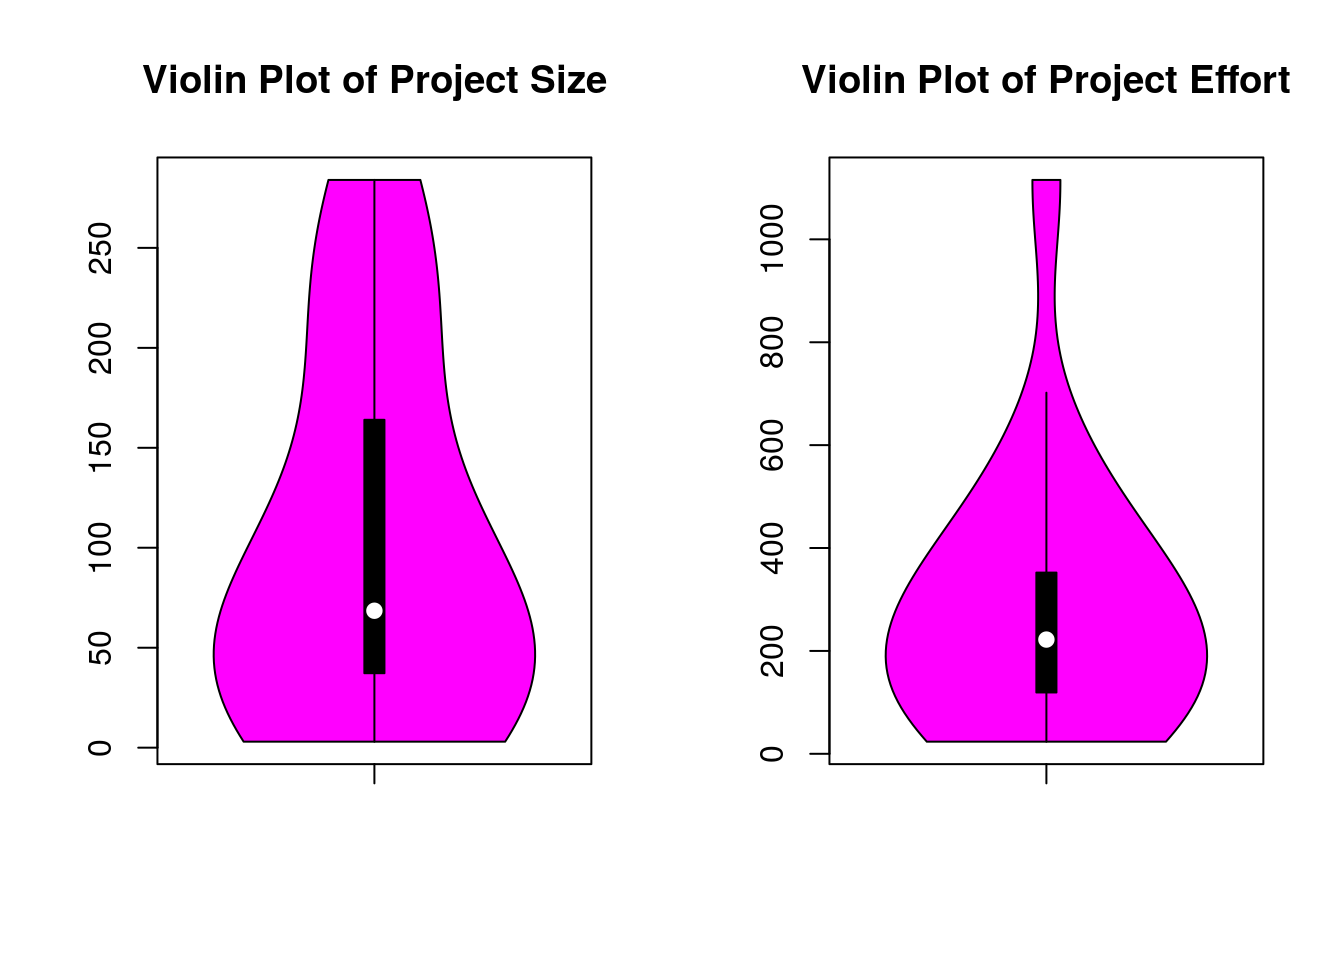
\includegraphics{DASE_files/figure-latex/unnamed-chunk-19-4.pdf}

\begin{Shaded}
\begin{Highlighting}[]
\KeywordTok{par}\NormalTok{(}\DataTypeTok{mfrow=}\KeywordTok{c}\NormalTok{(}\DecValTok{1}\NormalTok{,}\DecValTok{1}\NormalTok{))}
\KeywordTok{qqnorm}\NormalTok{(size_telecom1, }\DataTypeTok{main=}\StringTok{"Q-Q Plot of 'size'"}\NormalTok{)}
\KeywordTok{qqline}\NormalTok{(size_telecom1, }\DataTypeTok{col=}\DecValTok{2}\NormalTok{, }\DataTypeTok{lwd=}\DecValTok{2}\NormalTok{, }\DataTypeTok{lty=}\DecValTok{2}\NormalTok{) }\CommentTok{#draws a line through the first and third quartiles}
\end{Highlighting}
\end{Shaded}

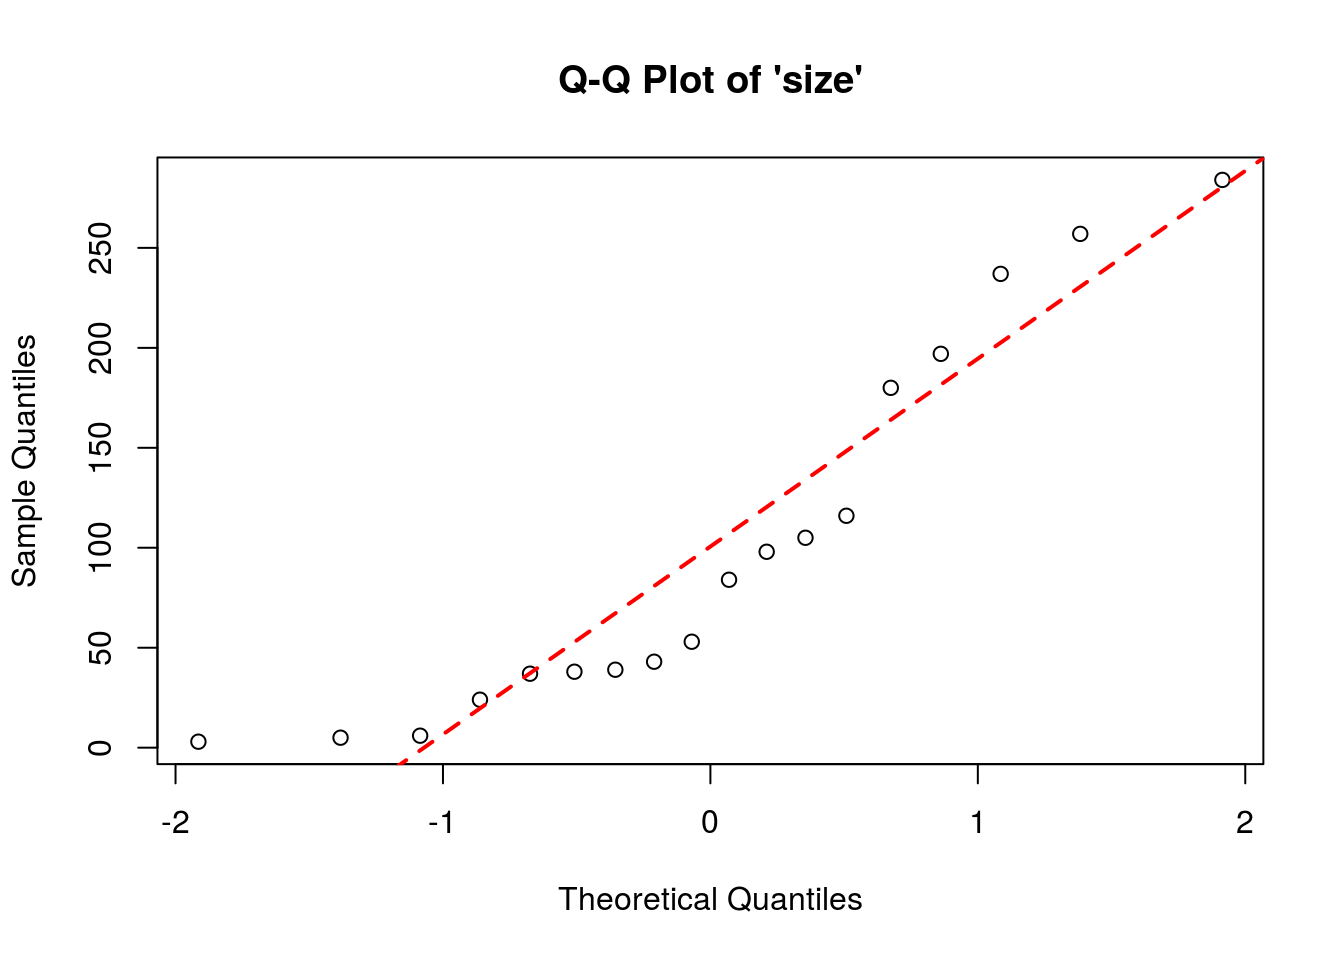
\includegraphics{DASE_files/figure-latex/unnamed-chunk-19-5.pdf}

\begin{Shaded}
\begin{Highlighting}[]
\KeywordTok{qqnorm}\NormalTok{(effort_telecom1,  }\DataTypeTok{main=}\StringTok{"Q-Q Plot of 'effort'"}\NormalTok{)}
\KeywordTok{qqline}\NormalTok{(effort_telecom1)}
\end{Highlighting}
\end{Shaded}

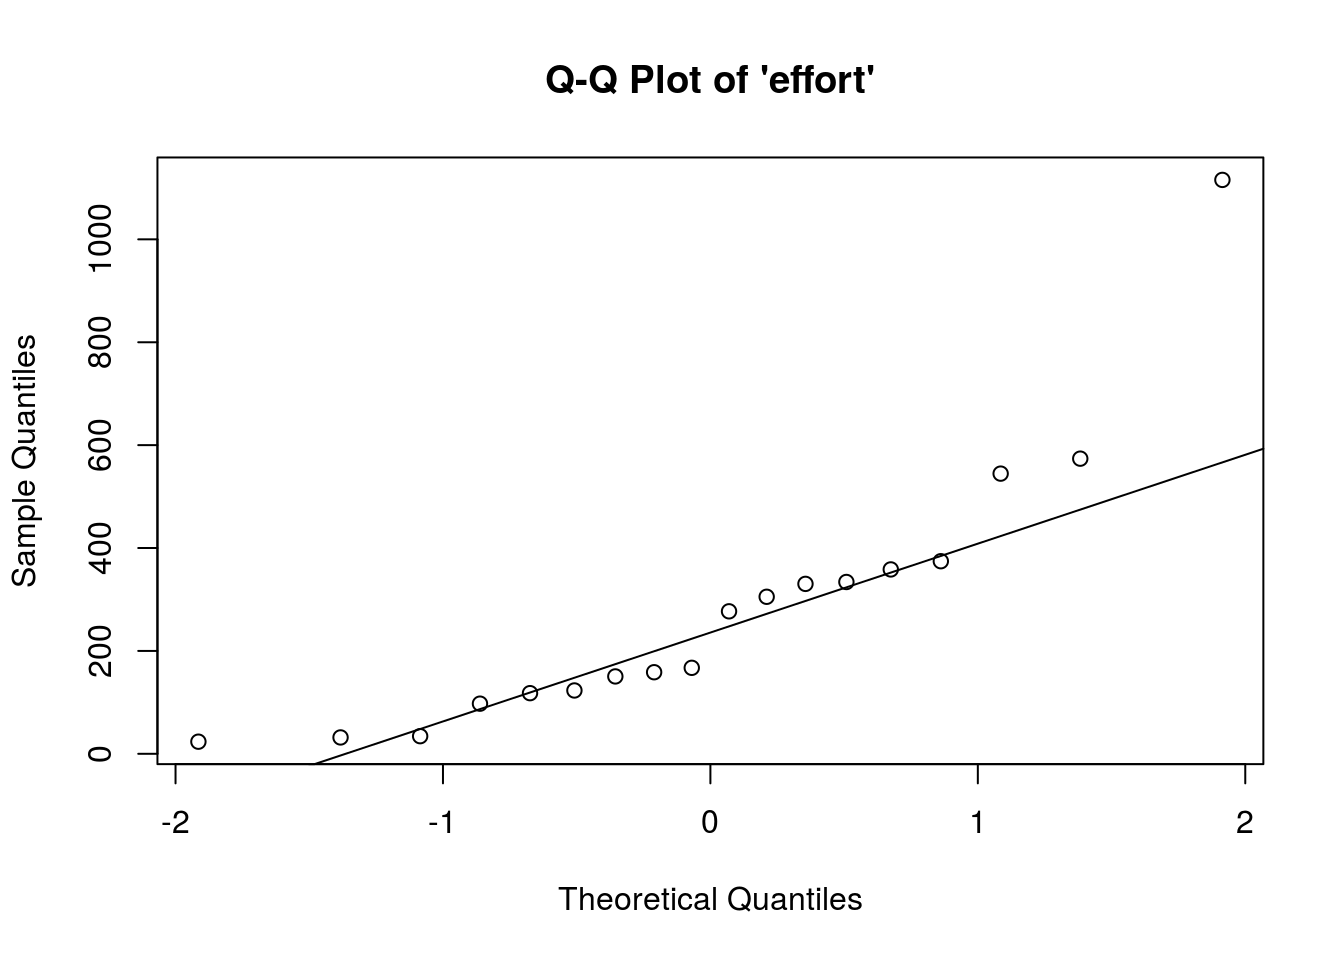
\includegraphics{DASE_files/figure-latex/unnamed-chunk-19-6.pdf} - We
observe the non-normality of the data.

\begin{itemize}
\tightlist
\item
  We may look the posible relationship between size and effort with a
  scatterplot
\end{itemize}

\begin{Shaded}
\begin{Highlighting}[]
\KeywordTok{plot}\NormalTok{(size_telecom1, effort_telecom1)}
\end{Highlighting}
\end{Shaded}

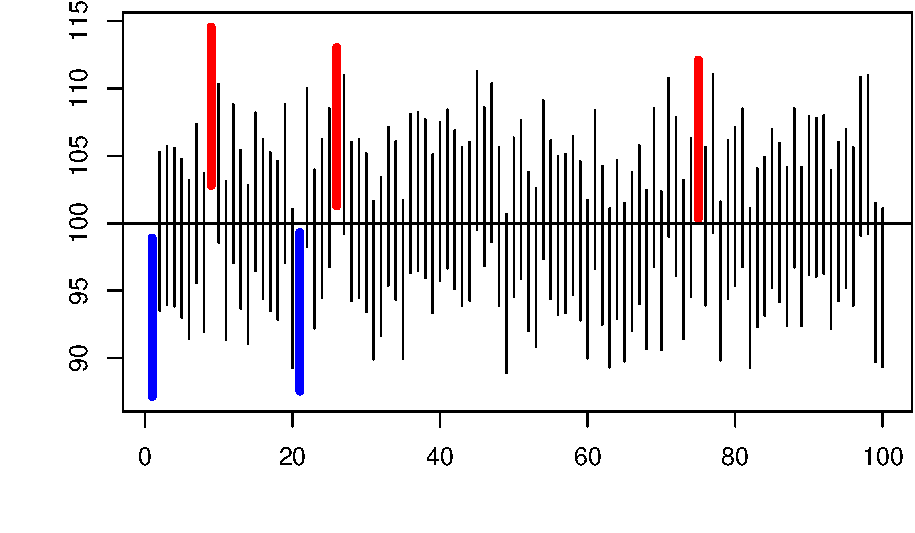
\includegraphics{DASE_files/figure-latex/unnamed-chunk-20-1.pdf}

\subsection{Example with the China dataset (Promise
Repository)}\label{example-with-the-china-dataset-promise-repository}

\begin{Shaded}
\begin{Highlighting}[]
\KeywordTok{library}\NormalTok{(foreign)}
\NormalTok{china <-}\StringTok{ }\KeywordTok{read.arff}\NormalTok{(}\StringTok{"./datasets/effortEstimation/china.arff"}\NormalTok{)}
\NormalTok{china_size <-}\StringTok{ }\NormalTok{china$AFP}
\KeywordTok{summary}\NormalTok{(china_size)}
\end{Highlighting}
\end{Shaded}

\begin{verbatim}
##    Min. 1st Qu.  Median    Mean 3rd Qu.    Max. 
##       9     100     215     487     438   17500
\end{verbatim}

\begin{Shaded}
\begin{Highlighting}[]
\NormalTok{china_effort <-}\StringTok{ }\NormalTok{china$Effort}
\KeywordTok{summary}\NormalTok{(china_effort)}
\end{Highlighting}
\end{Shaded}

\begin{verbatim}
##    Min. 1st Qu.  Median    Mean 3rd Qu.    Max. 
##      26     704    1830    3920    3830   54600
\end{verbatim}

\begin{Shaded}
\begin{Highlighting}[]
\KeywordTok{par}\NormalTok{(}\DataTypeTok{mfrow=}\KeywordTok{c}\NormalTok{(}\DecValTok{1}\NormalTok{,}\DecValTok{2}\NormalTok{))}
\KeywordTok{hist}\NormalTok{(china_size, }\DataTypeTok{col=}\StringTok{"blue"}\NormalTok{, }\DataTypeTok{xlab=}\StringTok{"Adjusted Function Points"}\NormalTok{, }\DataTypeTok{main=}\StringTok{"Distribution of AFP"}\NormalTok{)}
\KeywordTok{hist}\NormalTok{(china_effort, }\DataTypeTok{col=}\StringTok{"blue"}\NormalTok{,}\DataTypeTok{xlab=}\StringTok{"Effort"}\NormalTok{, }\DataTypeTok{main=}\StringTok{"Distribution of Effort"}\NormalTok{)}
\end{Highlighting}
\end{Shaded}

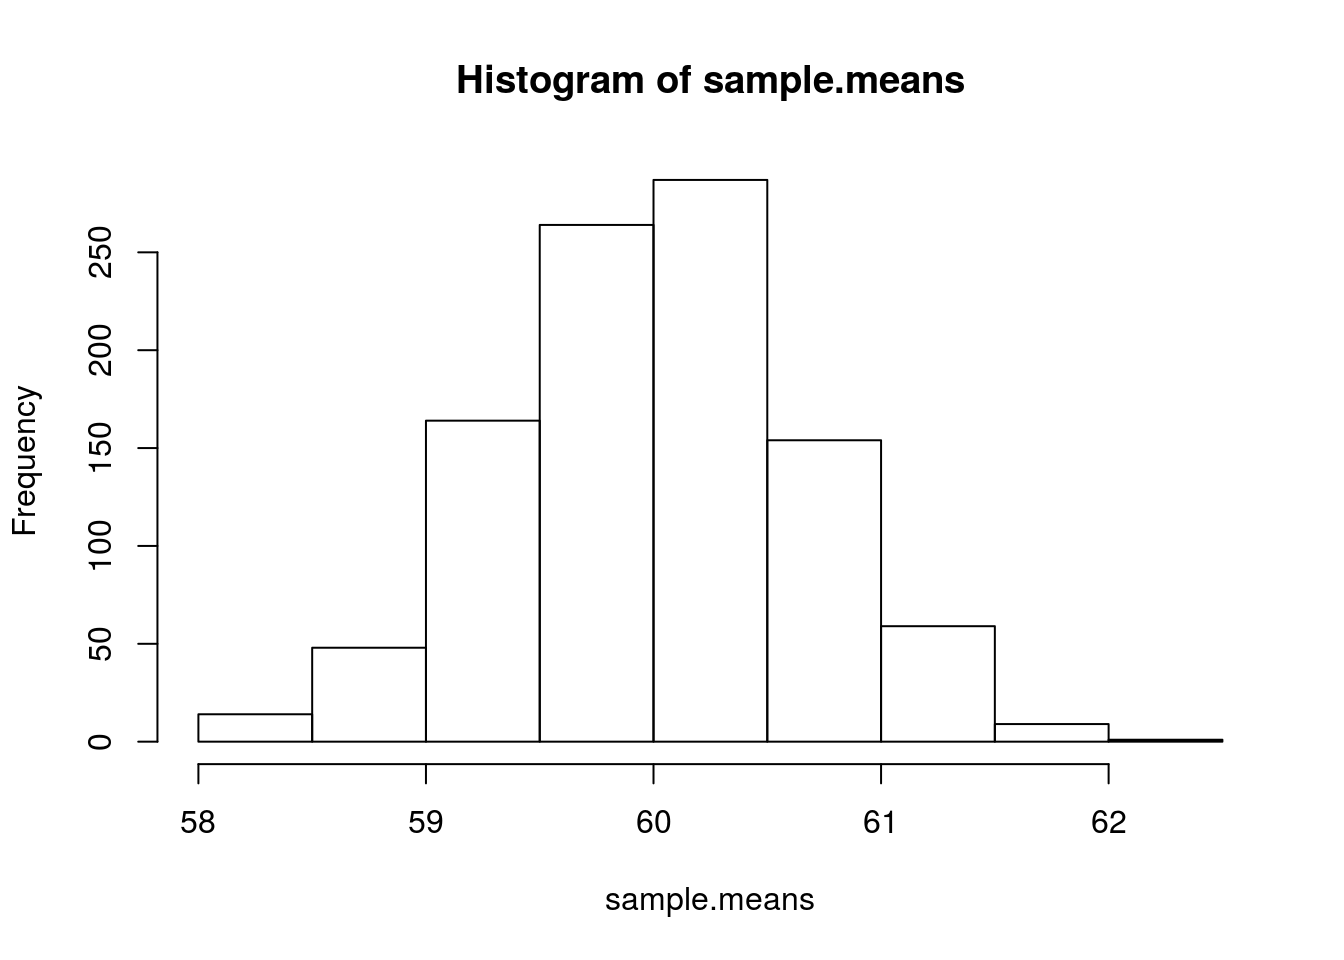
\includegraphics{DASE_files/figure-latex/unnamed-chunk-21-1.pdf}

\begin{Shaded}
\begin{Highlighting}[]
\KeywordTok{boxplot}\NormalTok{(china_size)}
\KeywordTok{boxplot}\NormalTok{(china_effort)}
\end{Highlighting}
\end{Shaded}

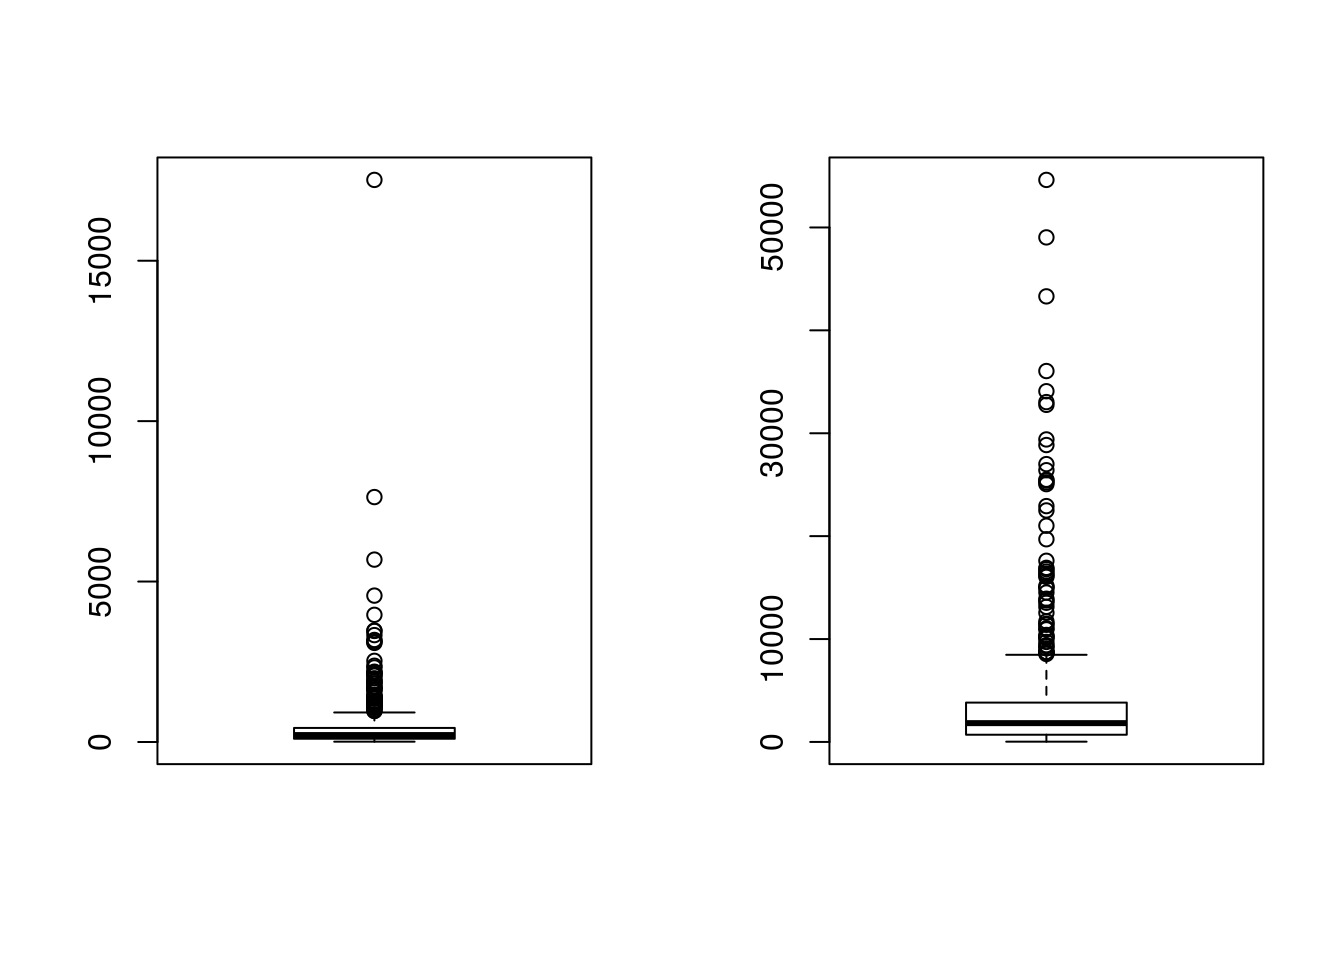
\includegraphics{DASE_files/figure-latex/unnamed-chunk-21-2.pdf}

\begin{Shaded}
\begin{Highlighting}[]
\KeywordTok{qqnorm}\NormalTok{(china_size)}
\KeywordTok{qqline}\NormalTok{(china_size)}
\KeywordTok{qqnorm}\NormalTok{(china_effort)}
\KeywordTok{qqline}\NormalTok{(china_effort)}
\end{Highlighting}
\end{Shaded}

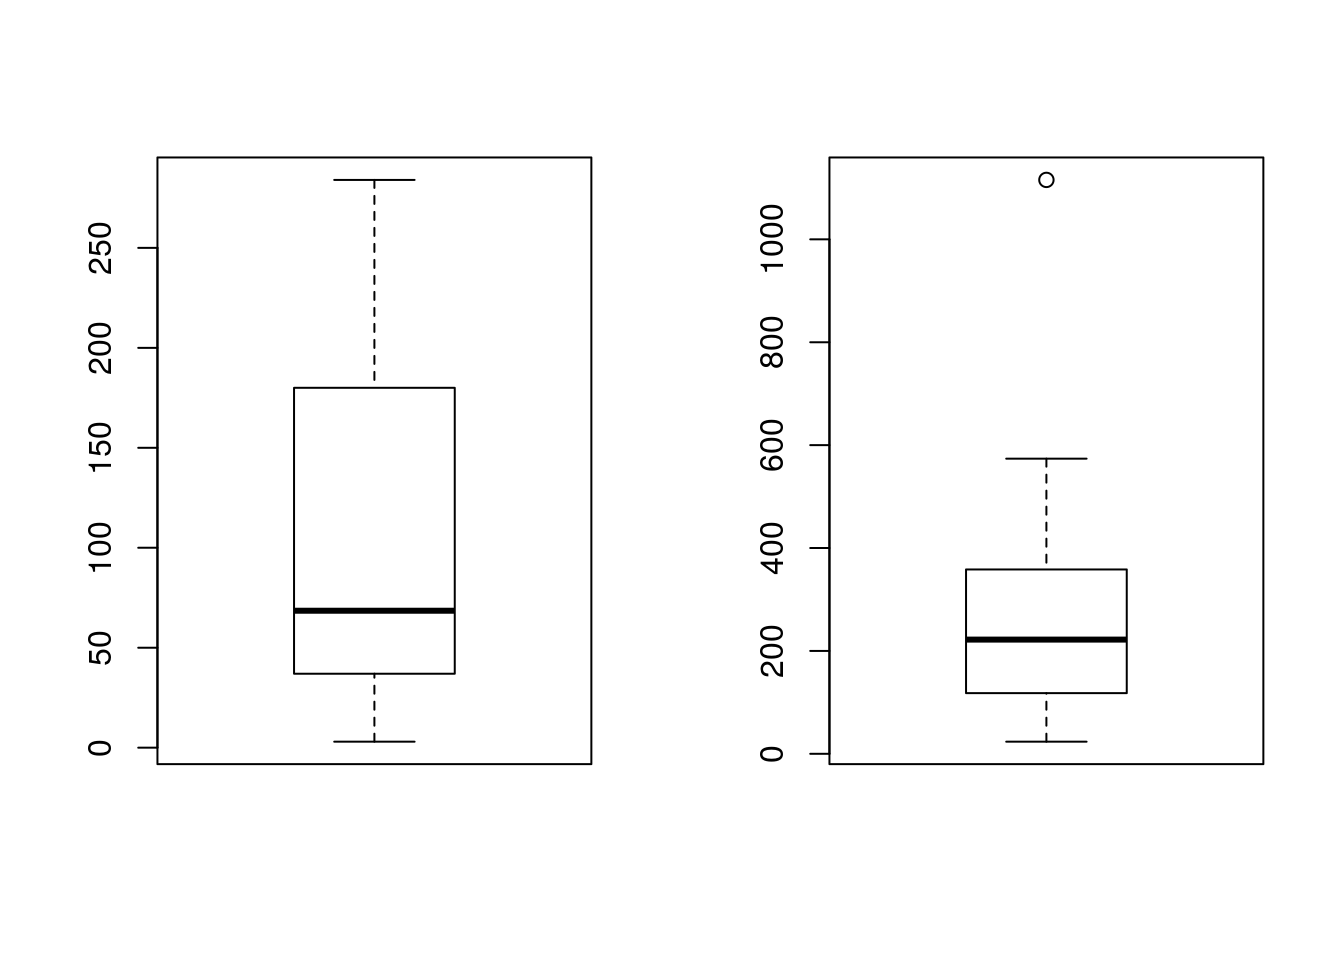
\includegraphics{DASE_files/figure-latex/unnamed-chunk-21-3.pdf} - We
observe the non-normality of the data.

\subsubsection{Normality. Galton data}\label{normality.-galton-data}

\begin{itemize}
\tightlist
\item
  It is the data based on the famous 1885 Francis Galton's study about
  the relationship between the heights of adult children and the heights
  of their parents.
\end{itemize}

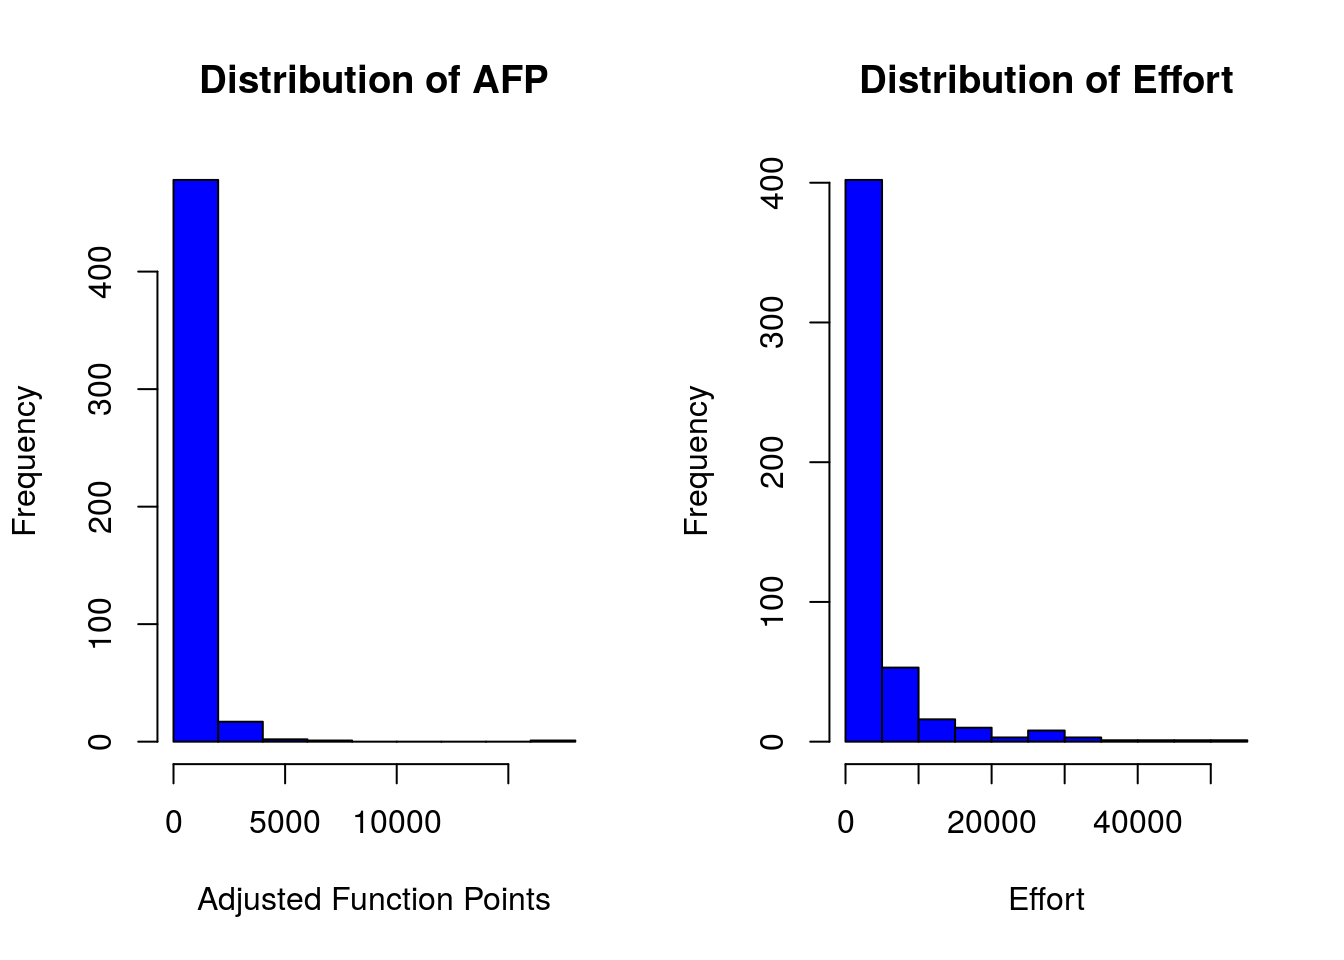
\includegraphics{DASE_files/figure-latex/unnamed-chunk-22-1.pdf}

\subsubsection{Normalization}\label{normalization}

\begin{itemize}
\tightlist
\item
  Take \(log\)s in both independent variables. For example, with the
  \emph{China} dataset.
\end{itemize}

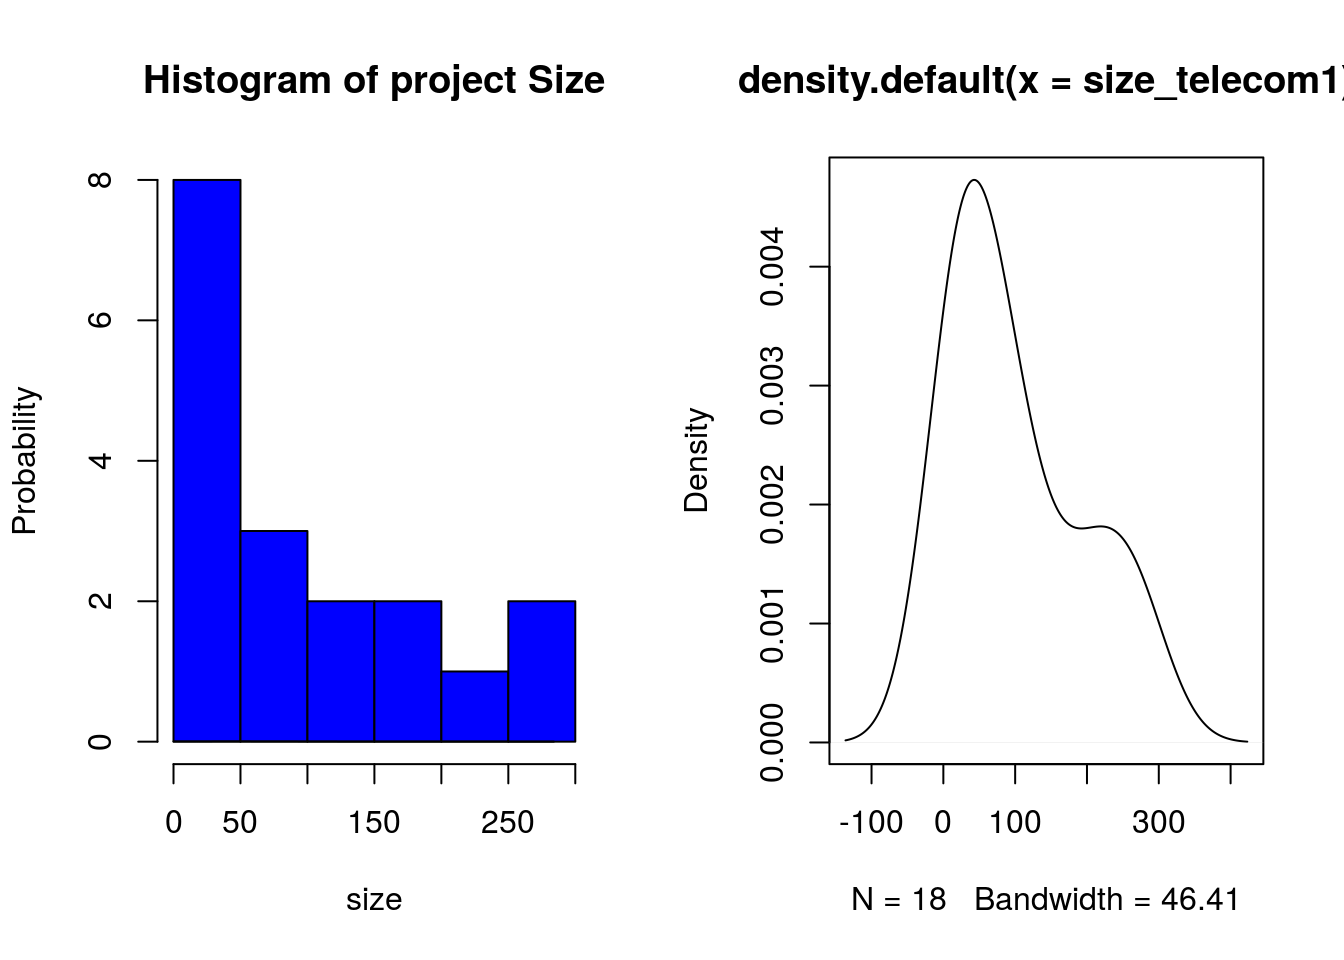
\includegraphics{DASE_files/figure-latex/unnamed-chunk-23-1.pdf}
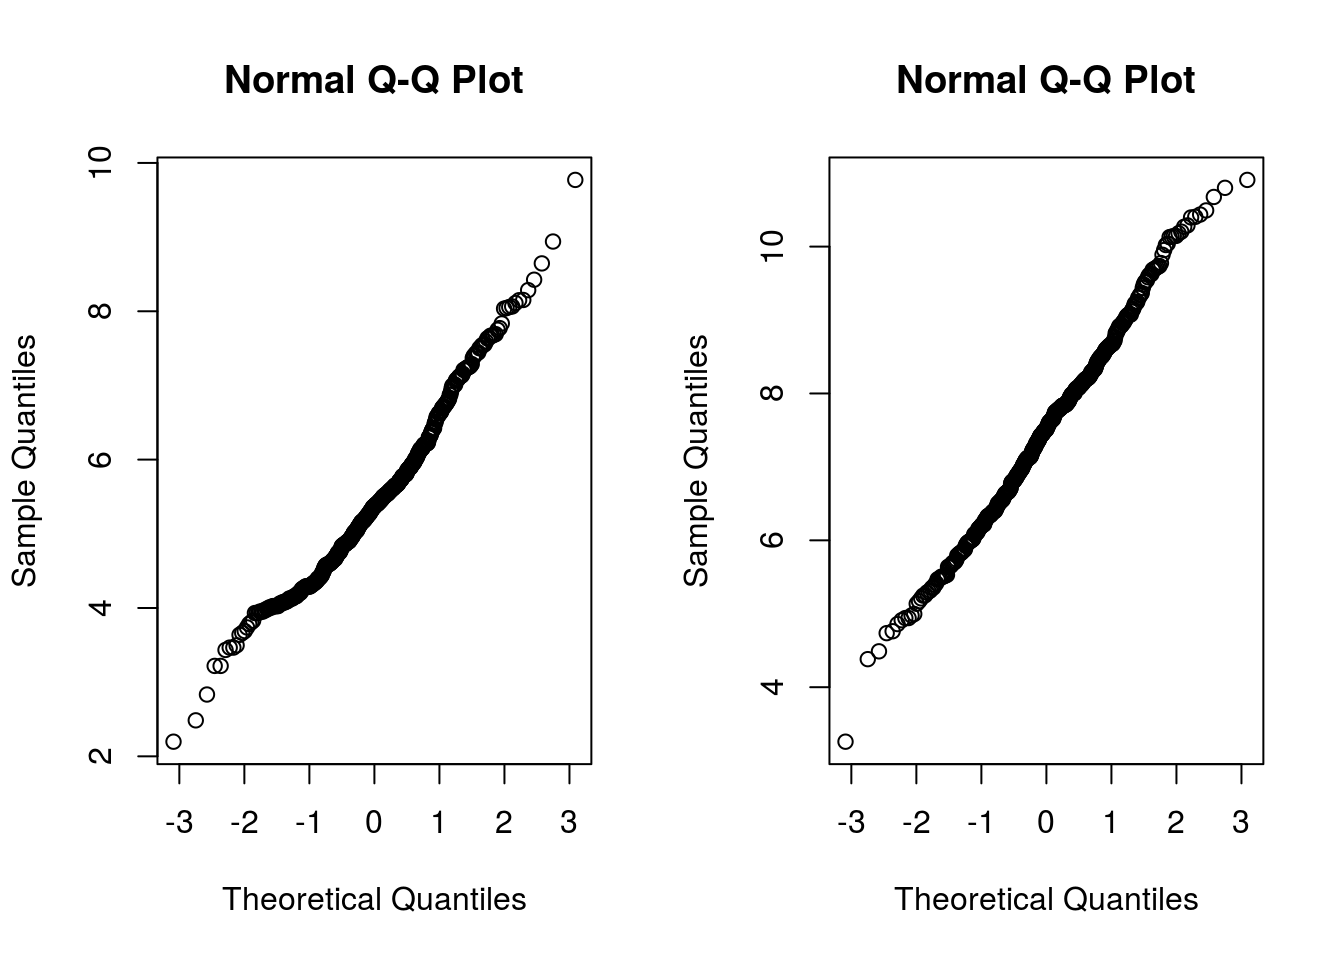
\includegraphics{DASE_files/figure-latex/unnamed-chunk-23-2.pdf}

\begin{itemize}
\tightlist
\item
  If the \(log\) transformation is used the estimation equation is:
  \[y= e^{b_0 + b_1 log(x)} \]
\end{itemize}

\section{Correlation}\label{correlation}

\begin{itemize}
\tightlist
\item
  \textbf{Correlation} is a statistical relationship between two sets of
  data.
\item
  With the whole dataset we may check for the linear Correlation of the
  variables we are interested in.
\end{itemize}

As an example with the China dataset

\begin{Shaded}
\begin{Highlighting}[]
\KeywordTok{par}\NormalTok{(}\DataTypeTok{mfrow=}\KeywordTok{c}\NormalTok{(}\DecValTok{1}\NormalTok{,}\DecValTok{1}\NormalTok{))}
\KeywordTok{plot}\NormalTok{(china_size,china_effort)}
\end{Highlighting}
\end{Shaded}

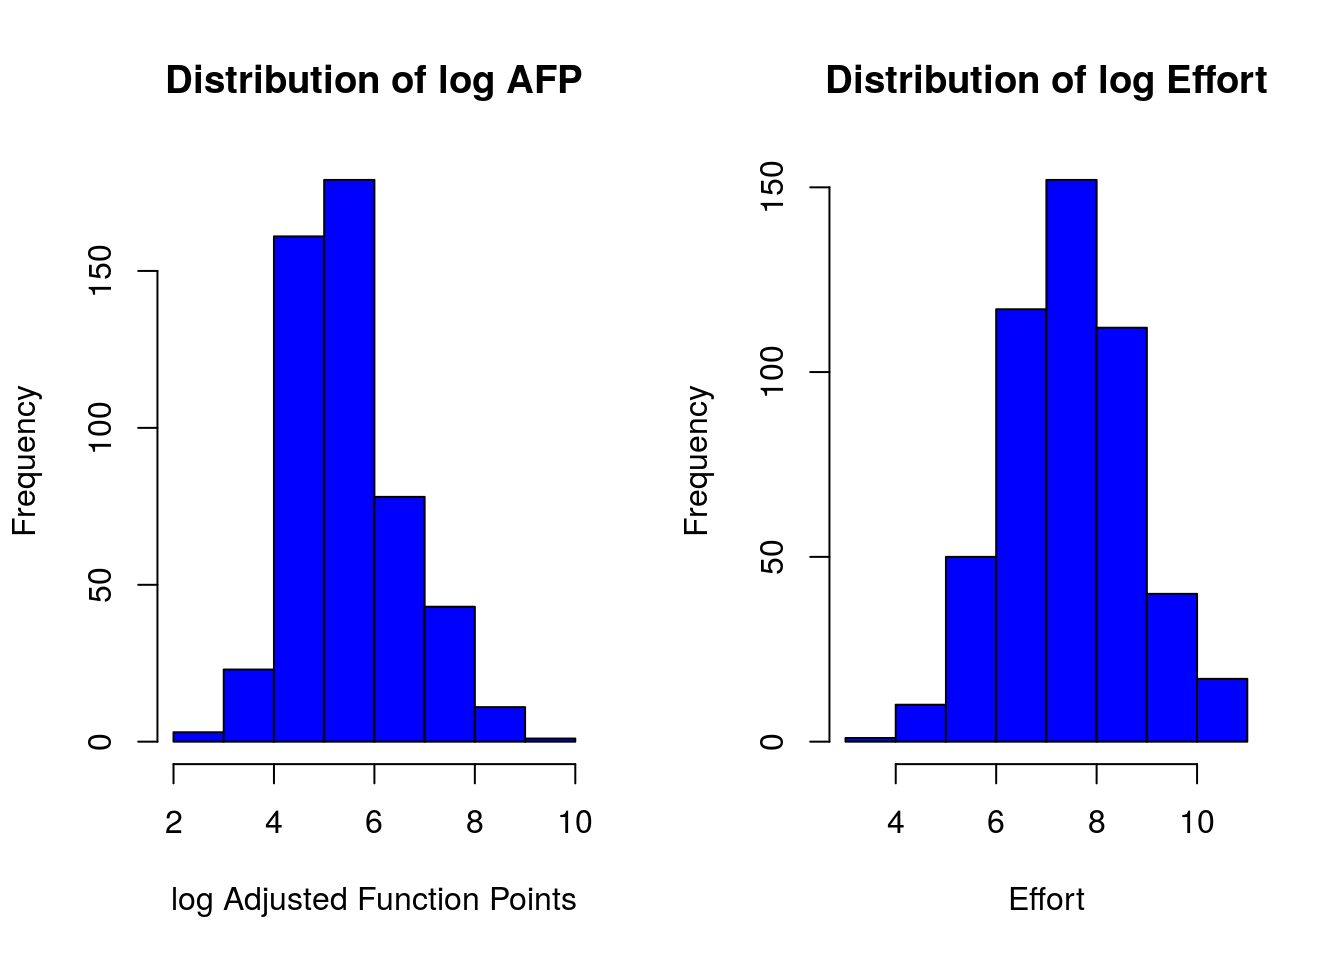
\includegraphics{DASE_files/figure-latex/unnamed-chunk-24-1.pdf}

\begin{Shaded}
\begin{Highlighting}[]
\KeywordTok{cor}\NormalTok{(china_size,china_effort)}
\end{Highlighting}
\end{Shaded}

\begin{verbatim}
## [1] 0.685
\end{verbatim}

\begin{Shaded}
\begin{Highlighting}[]
\KeywordTok{cor.test}\NormalTok{(china_size,china_effort)}
\end{Highlighting}
\end{Shaded}

\begin{verbatim}
## 
##  Pearson's product-moment correlation
## 
## data:  china_size and china_effort
## t = 20, df = 500, p-value <2e-16
## alternative hypothesis: true correlation is not equal to 0
## 95 percent confidence interval:
##  0.635 0.729
## sample estimates:
##   cor 
## 0.685
\end{verbatim}

\begin{Shaded}
\begin{Highlighting}[]
\KeywordTok{cor}\NormalTok{(china_size,china_effort, }\DataTypeTok{method=}\StringTok{"spearman"}\NormalTok{)}
\end{Highlighting}
\end{Shaded}

\begin{verbatim}
## [1] 0.649
\end{verbatim}

\begin{Shaded}
\begin{Highlighting}[]
\KeywordTok{cor}\NormalTok{(china_size,china_effort, }\DataTypeTok{method=}\StringTok{"kendall"}\NormalTok{)}
\end{Highlighting}
\end{Shaded}

\begin{verbatim}
## [1] 0.468
\end{verbatim}

\section{Confidence Intervals.
Bootstrap}\label{confidence-intervals.-bootstrap}

\begin{itemize}
\tightlist
\item
  Until now we have generated point estimates
\item
  A \emph{confidence interval} (CI) is an interval estimate of a
  population parameter. The parameter can be the mean, the median or
  other. The frequentist CI is an observed interval that is different
  from sample to sample. It frequently includes the value of the
  unobservable parameter of interes if the experiment is repeated. The
  \emph{confidence level} is the value that measures the frequency that
  the constructed intervals contain the true value of the parameter.
\item
  The construction of a confidence interval with an exact value of
  confidence level for a distribution requires some statistical
  properties. Usually, \emph{normality} is one of the properties
  required for computing confidence intervals.

  \begin{itemize}
  \tightlist
  \item
    Not all confidence intervals contain the true value of the
    parameter.
  \item
    Simulation of confidence intervals
  \end{itemize}
\end{itemize}

An example from Ugarte et al. \citep{ugarte2015probability}

\begin{Shaded}
\begin{Highlighting}[]
\KeywordTok{set.seed}\NormalTok{(}\DecValTok{10}\NormalTok{)}
\KeywordTok{norsim}\NormalTok{(}\DataTypeTok{sims =} \DecValTok{100}\NormalTok{, }\DataTypeTok{n =} \DecValTok{36}\NormalTok{, }\DataTypeTok{mu =} \DecValTok{100}\NormalTok{, }\DataTypeTok{sigma =} \DecValTok{18}\NormalTok{, }\DataTypeTok{conf.level =} \FloatTok{0.95}\NormalTok{)}
\end{Highlighting}
\end{Shaded}

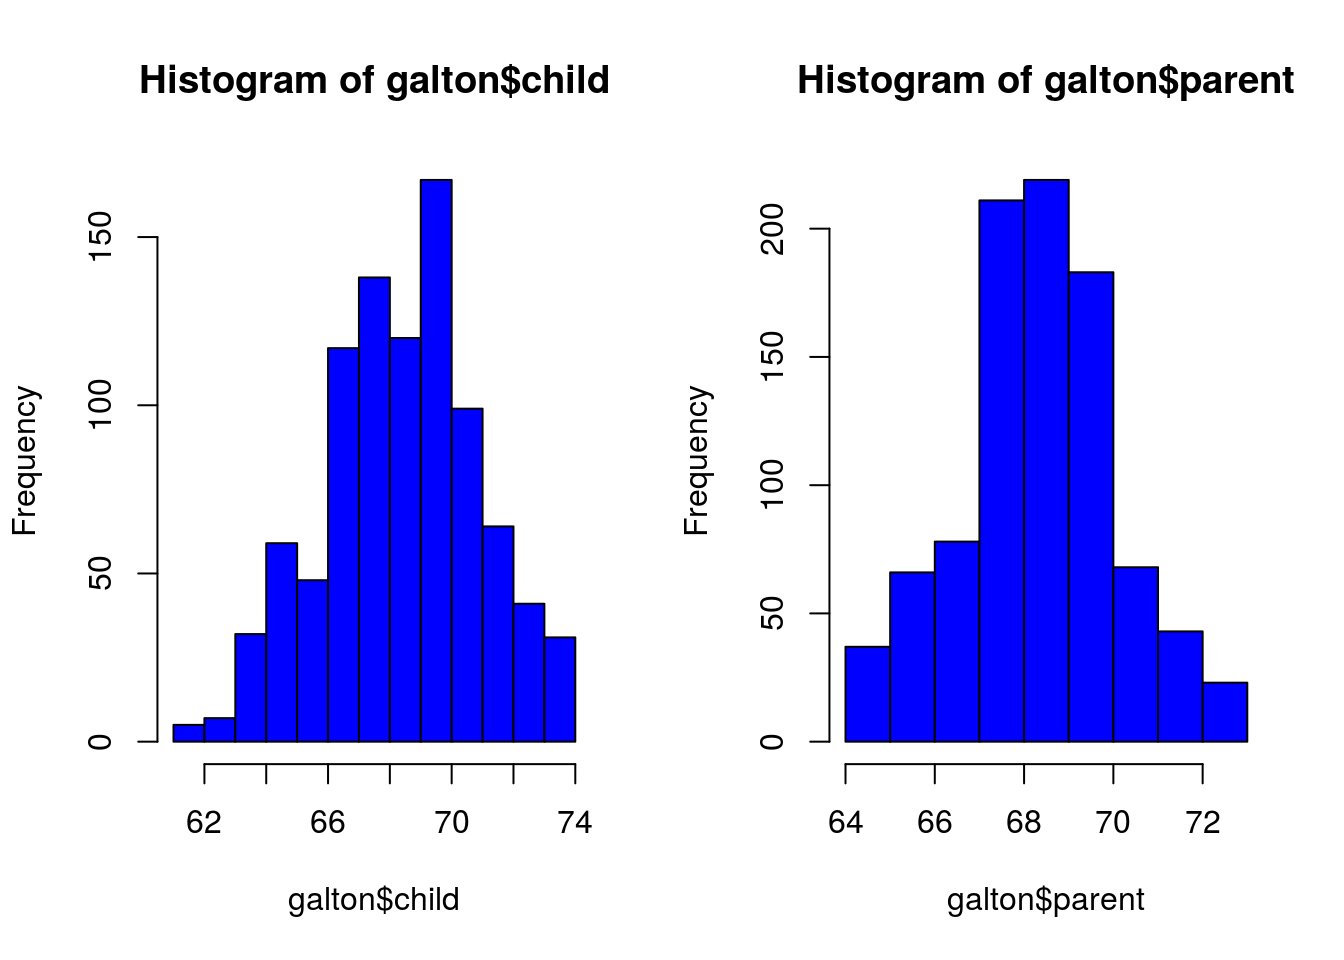
\includegraphics{DASE_files/figure-latex/unnamed-chunk-26-1.pdf}

\begin{itemize}
\tightlist
\item
  The range defined by the confidence interval will vary with each
  sample, because the sample size will vary each time and the standard
  deviation will vary too.
\item
  95\% confidence interval: it is the probability that the hypothetical
  confidence intervals (that would be computed from the hypothetical
  repeated samples) will contain the population mean.
\item
  the particular interval that we compute on one sample does not mean
  that the population mean lies within that interval with a probability
  of 95\%.
\item
  Recommended reading: \citep{Hoekstra2014} \emph{Robust
  misinterpretation of confidence intervals}
\end{itemize}

\section{Nonparametric Bootstrap}\label{nonparametric-bootstrap}

\begin{itemize}
\tightlist
\item
  For computing CIs the important thing is to know the assumptions that
  are made to ``know'' the distribution of the statistic.
\item
  There is a way to compute confidence intervals without meeting the
  requirements of parametric methods.
\item
  \textbf{Resampling} or \textbf{bootstraping} is a method to calculate
  estimates of a parameter taking samples from the original data and
  using those \emph{resamples} to calculate statistics. Using the
  resamples usually gives more accurate results than using the original
  single sample to calculate an estimate of a parameter.
\end{itemize}

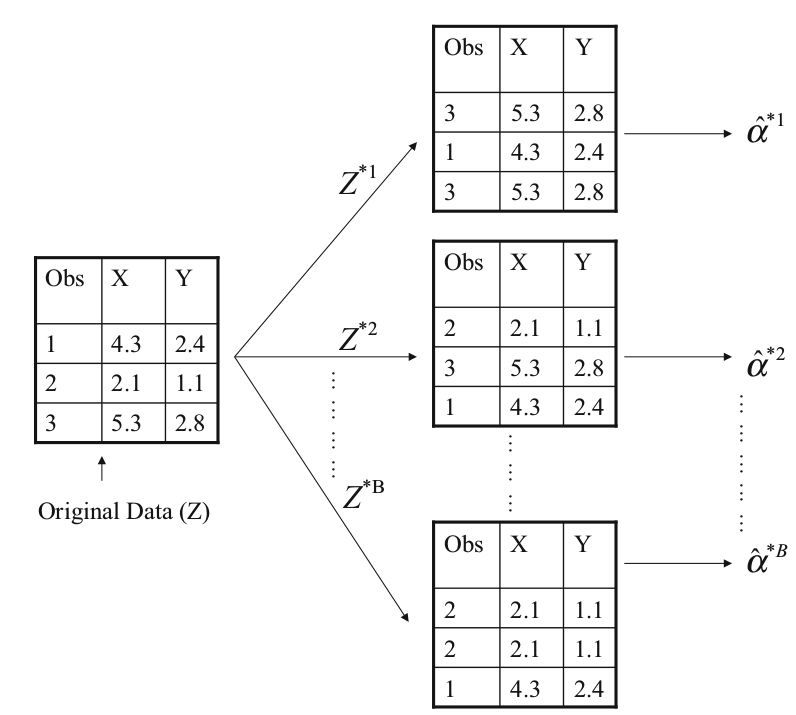
\includegraphics{figures/bootstrap.png} - An example of bootstrap CI can
be found in Chapter \ref{evaluationSE}, ``Evaluation in Software
Engineering''

\chapter{Classical Hypothesis
Testing}\label{classical-hypothesis-testing}

\begin{itemize}
\item
  By ``classical'' we mean the standard ``frequentist'' approach to
  hypothesis testing. The ``frequentist'' approach to probability sees
  it as the frequency of events in the long run. We repeat experiments
  over and over and we count the times that our object of interest
  appears in the sequence.
\item
  The classical approach is usually called \textbf{null hypothesis
  significance testing} (NHST) because the process starts by setting a
  null hypothesis \(H_0\) which is the opposite about what we think is
  true.
\item
  The rationale of the process is that the statistical hypothesis should
  be \emph{falsifiable}, that is, we can find evidence that the
  hypothesis is not true. We try to find evidence against the null
  hypothesis in order to support our alternative hypothesis \(H_A\)
\item
  Usually, the null hypothesis is described as the situation of ``no
  effect'' and the alternative hypothesis describes the effect that we
  are looking for.
\item
  After collecting data, taking an actual sample, we measure the
  distance of our parameter of interest from the hypothesized population
  parameter, and use the facts of the sampling distribution to determine
  the probability of obtaining such a sample \emph{assuming the
  hypothesis is true}. This is amounts to a test of the hypothesis.
\item
  If the probability of our sample, given the null hypothesis is high,
  this provides evidence that the null hypothesis is true. Conversely,
  if the probability of the sample is low (given the hypothesis), this
  is evidence against the null hypothesis. The hypothesis being tested
  in this way is named the \emph{null hypothesis}.
\item
  The goal of the test is to determine if the null hypothesis can be
  rejected. A statistical test can either reject or fail to reject a
  null hypothesis, but never prove it true.
\item
  We can make two types of errors: false positive (Type I) and false
  negative (Type II)
\item
  Type I and Type II errors

  \begin{figure}[htbp]
  \centering
  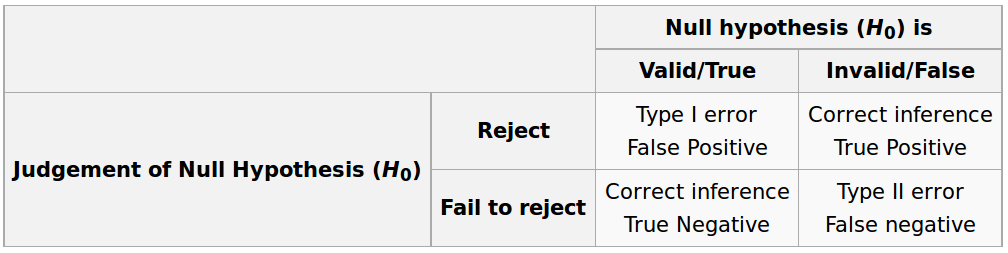
\includegraphics{figures/typeIandIIwiki.png}
  \caption{}
  \end{figure}
\item
  Two-tailed NHST

  \begin{figure}[htbp]
  \centering
  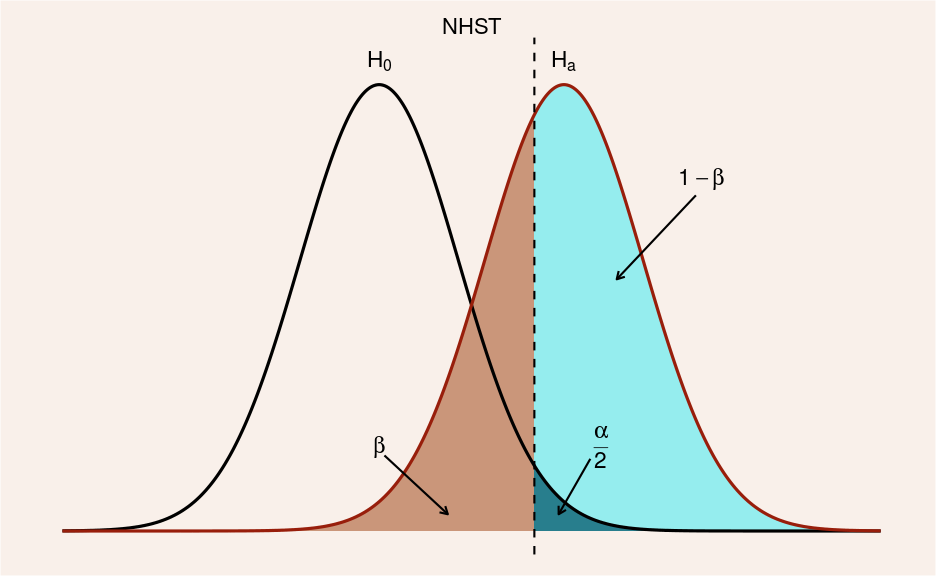
\includegraphics{figures/stat_power_ggplot.png}
  \caption{}
  \end{figure}
\item
  One-tailed NHST

  \begin{figure}[htbp]
  \centering
  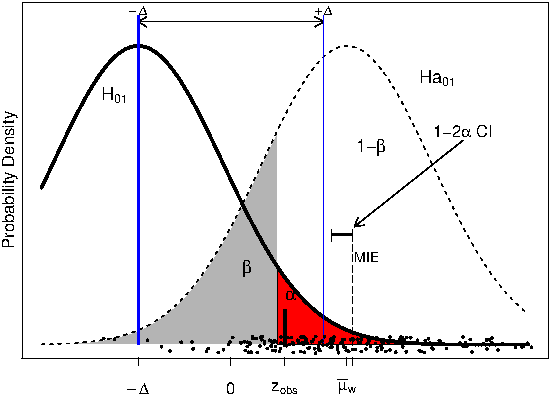
\includegraphics{figures/One-tailedNHST.png}
  \caption{}
  \end{figure}
\item
  elementary example
\end{itemize}

\begin{Shaded}
\begin{Highlighting}[]
\NormalTok{data =}\StringTok{ }\KeywordTok{c}\NormalTok{(}\FloatTok{52.7}\NormalTok{, }\FloatTok{53.9}\NormalTok{, }\FloatTok{41.7}\NormalTok{, }\FloatTok{71.5}\NormalTok{, }\FloatTok{47.6}\NormalTok{, }\FloatTok{55.1}\NormalTok{, }\FloatTok{62.2}\NormalTok{, }\FloatTok{56.5}\NormalTok{, }\FloatTok{33.4}\NormalTok{, }\FloatTok{61.8}\NormalTok{, }\FloatTok{54.3}\NormalTok{, }\FloatTok{50.0}\NormalTok{, }\FloatTok{45.3}\NormalTok{, }\FloatTok{63.4}\NormalTok{, }\FloatTok{53.9}\NormalTok{, }\FloatTok{65.5}\NormalTok{, }\FloatTok{66.6}\NormalTok{, }\FloatTok{70.0}\NormalTok{, }\FloatTok{52.4}\NormalTok{, }\FloatTok{38.6}\NormalTok{, }\FloatTok{46.1}\NormalTok{, }\FloatTok{44.4}\NormalTok{, }\FloatTok{60.7}\NormalTok{, }\FloatTok{56.4}\NormalTok{);}
\KeywordTok{t.test}\NormalTok{(data, }\DataTypeTok{mu=}\DecValTok{50}\NormalTok{, }\DataTypeTok{alternative =} \StringTok{'greater'}\NormalTok{)}
\end{Highlighting}
\end{Shaded}

\begin{verbatim}
## 
##  One Sample t-test
## 
## data:  data
## t = 2, df = 20, p-value = 0.02
## alternative hypothesis: true mean is greater than 50
## 95 percent confidence interval:
##  50.9  Inf
## sample estimates:
## mean of x 
##      54.3
\end{verbatim}

\begin{itemize}
\item
  Keeping this simple, we could start hypothesis testing about one
  sample median with the wilcoxon test for non-normal distributions.
\item
  ``ae'' is the absolute error in the China Test data
\end{itemize}

\begin{Shaded}
\begin{Highlighting}[]
\KeywordTok{median}\NormalTok{(ae)}
\end{Highlighting}
\end{Shaded}

\begin{verbatim}
## [1] 867
\end{verbatim}

\begin{Shaded}
\begin{Highlighting}[]
\KeywordTok{mean}\NormalTok{(ae)}
\end{Highlighting}
\end{Shaded}

\begin{verbatim}
## [1] 1867
\end{verbatim}

\begin{Shaded}
\begin{Highlighting}[]
\KeywordTok{wilcox.test}\NormalTok{(ae, }\DataTypeTok{mu=}\DecValTok{800}\NormalTok{, }\DataTypeTok{alternative =} \StringTok{'greater'}\NormalTok{) }\CommentTok{#change the values of mu and see the results}
\end{Highlighting}
\end{Shaded}

\begin{verbatim}
## 
##  Wilcoxon signed rank test with continuity correction
## 
## data:  ae
## V = 9000, p-value = 8e-04
## alternative hypothesis: true location is greater than 800
\end{verbatim}

\begin{itemize}
\tightlist
\item
  Quick introduction at
  \url{https://psychstatsworkshop.wordpress.com/2014/08/06/lesson-9-hypothesis-testing/}
\end{itemize}

\section{p-values}\label{p-values}

\begin{itemize}
\tightlist
\item
  p-value: the p-value of a statistical test is the probability,
  computed assuming that \(H_0\) is true, that the test statistic would
  take a value as extreme or more extreme than that actually observed.
\item
  \url{http://www.nature.com/news/psychology-journal-bans-p-values-1.17001}
\item
  \url{https://www.sciencenews.org/blog/context/p-value-ban-small-step-journal-giant-leap-science}
\end{itemize}

\begin{figure}[htbp]
\centering

\includegraphics{figures/pvalueBan.png}
\caption{}
\end{figure}

\part{Preprocessing}\label{part-preprocessing}

\chapter{Preprocessing}\label{preprocessing}

Following the data mining process, we describe what is meant by
preprocessing, classical supervised models, unsupervised models and
evaluation in the context of software engineering with examples

This task is probably the hardest and where most of effort is spend in
the data mining process. It is quite typical to transform the data, for
example, finding inconsistencies, normalising, imputing missing values,
tranforming input data, merging variables, etc.

Typically, preprocessing consist of the following tasks (subprocesses):

\begin{itemize}
\tightlist
\item
  Data cleaning (consistency, noise detection, outliers)
\item
  Data integration
\item
  Data transformation (normalisation, discretisation) and derivation of
  new attributes from existing ones (e.g., population density from
  population and area)
\item
  Missing data imputation
\item
  Data reduction (feature selection and instace selection)
\end{itemize}

\section{Data}\label{data}

\emph{Consistent} data are semantically correct based on real-world
knowledge of the problem, i.e., no constrains are violated and data that
can be used for inducing models and analysis. For example, the LoC or
effort is constrained to non-negative values. We can also consider that
to multiple attributes are consistent among them, and even datasets
(e.g., same metrics but collected by different tools)

\section{Missing values}\label{missing-values}

Three types of problems are usually associated with MVs in DM {[}5{]}:

\begin{enumerate}
\def\labelenumi{\arabic{enumi}.}
\tightlist
\item
  loss of efficiency
\item
  complications in handling and analyzing the data
\item
  bias resulting from differences between missing and complete data.
\end{enumerate}

Imputation consists in replacing missing values for estimates of those
missing values. Many algorithms do cannot handle missing values and
imputation methods are needed.

In R, a missing value is represented with \texttt{NA} and the analyst
must decide what to do with missing data. The simplest approach is to
leave out instances (ignore missing -IM-) with with missing data. This
functionality is supported by many base functions through the
\texttt{na.rm} option.

\section{Imputation methods}\label{imputation-methods}

We can use simple approaches such as the replacing the missing values
with the mean or mode of the attribute.

More elaborated approaches include:

\begin{itemize}
\tightlist
\item
  EM (Expectation-Maximisation)
\item
  Distance-based

  \begin{itemize}
  \tightlist
  \item
    kNN (k Nearest Neighbours)
  \item
    Clustering
  \end{itemize}
\end{itemize}

\section{Noise}\label{noise}

Imperfections of the real-world data that influences negatively in the
induced machine learning models. Approaches to deal with noisy data: *
Robust learners capable of handling noisy data (e.g., C4.5 through
pruning strategies) * Data polishing methods which aim to correct noisy
instances prior training * Noise filters which are used to identify and
eliminate noisy instances from the training data.

Types of noise data: * Class Noise (aka label noise). + There can be
contradictory cases (all attributes have the same value except the
class) + Misclassifications. The class attribute is not labeled with the
true label (golden truth) * Attribute Noise. Values of attributes that
are noise, missing or unknown.

\section{Outliers}\label{outliers}

There is a large amount of literature related to outlier detection, and
furthermore several definitions of outlier exist.

\begin{Shaded}
\begin{Highlighting}[]
\KeywordTok{library}\NormalTok{(DMwR)}
\KeywordTok{library}\NormalTok{(foreign)}

\NormalTok{kc1 <-}\StringTok{ }\KeywordTok{read.arff}\NormalTok{(}\StringTok{"./datasets/defectPred/D1/KC1.arff"}\NormalTok{)}
\end{Highlighting}
\end{Shaded}

The LOF algorithm (\texttt{lofactor}), given a data set it produces a
vector of local outlier factors for each case.

\begin{Shaded}
\begin{Highlighting}[]
\NormalTok{kc1num <-}\StringTok{ }\NormalTok{kc1[,}\DecValTok{1}\NormalTok{:}\DecValTok{21}\NormalTok{]}
\NormalTok{outlier.scores <-}\StringTok{ }\KeywordTok{lofactor}\NormalTok{(kc1num, }\DataTypeTok{k=}\DecValTok{5}\NormalTok{)}
\KeywordTok{plot}\NormalTok{(}\KeywordTok{density}\NormalTok{(}\KeywordTok{na.omit}\NormalTok{(outlier.scores)))}
\end{Highlighting}
\end{Shaded}

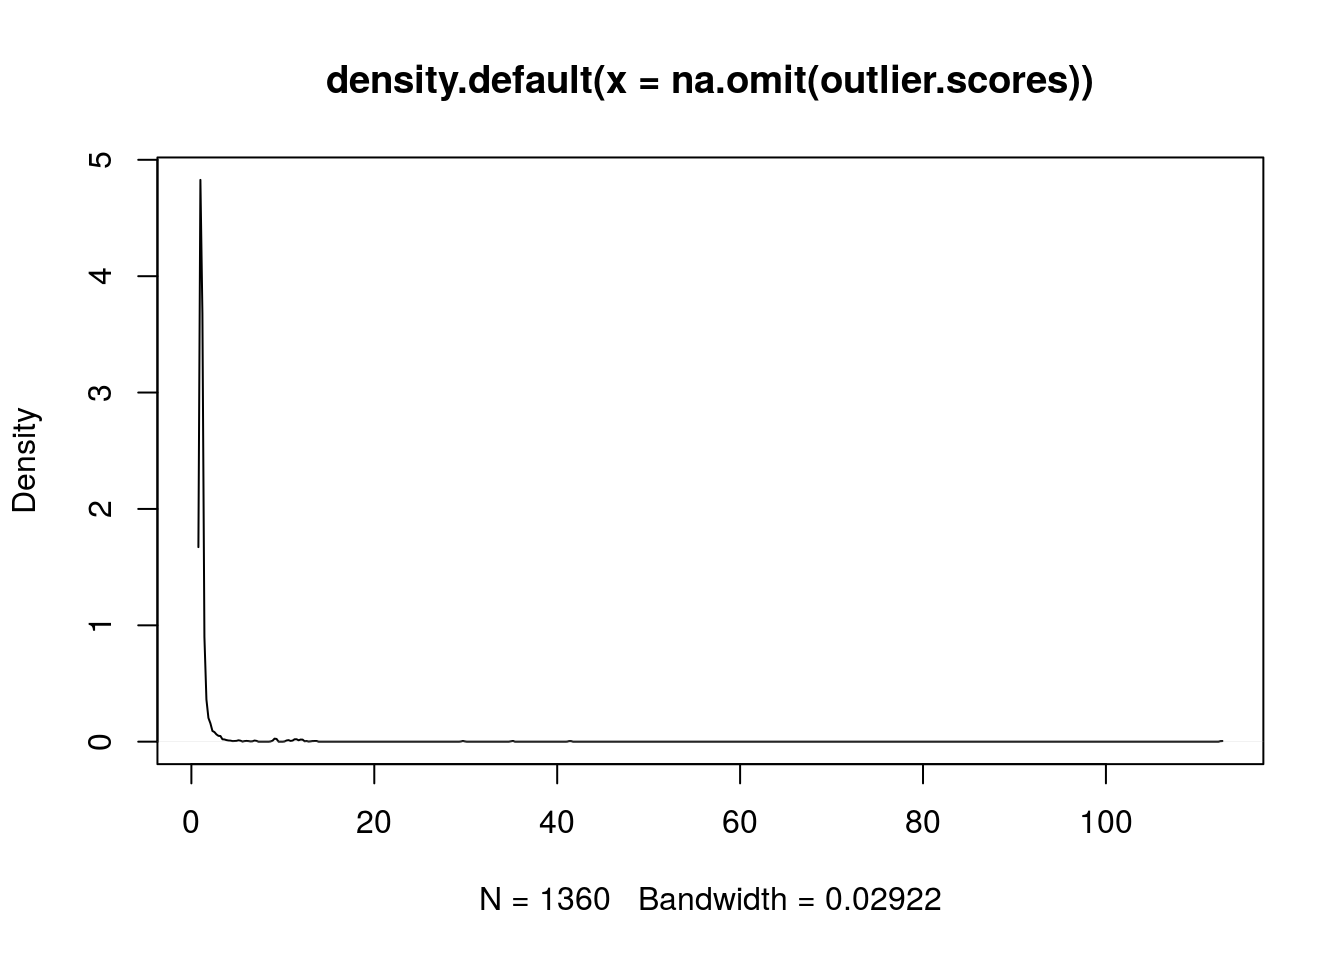
\includegraphics{DASE_files/figure-latex/unnamed-chunk-31-1.pdf}

\begin{Shaded}
\begin{Highlighting}[]
\NormalTok{outliers <-}\StringTok{ }\KeywordTok{order}\NormalTok{(outlier.scores, }\DataTypeTok{decreasing=}\NormalTok{T)[}\DecValTok{1}\NormalTok{:}\DecValTok{5}\NormalTok{]}
\KeywordTok{print}\NormalTok{(outliers)}
\end{Highlighting}
\end{Shaded}

\begin{verbatim}
## [1]  1  6 14 31 33
\end{verbatim}

Another simple method of Hiridoglou and Berthelot for positive
observations.

\section{Feature selection}\label{feature-selection}

Feature Selection (FS) aims at identifying the most relevant attributes
from a dataset. It is important in different ways:

\begin{itemize}
\item
  A reduced volume of data allows different data mining or searching
  techniques to be applied.
\item
  Irrelevant and redundant attributes can generate less accurate and
  more complex models. Furthermore, data mining algorithms can be
  executed faster.
\item
  It avoids the collection of data for those irrelevant and redundant
  attributes in the future.
\end{itemize}

The problem of FS received a thorough treatment in pattern recognition
and machine learning. Most of the FS algorithms tackle the task as a
\emph{search} problem, where each state in the search specifies a
distinct subset of the possible attributes \citep{BL97}. The search
procedure is combined with a criterion to evaluate the merit of each
candidate subset of attributes. There are a multiple possible
combinations between each procedure search and each attribute measure
\citep{LY05}.

There are two major approaches in FS from the method's output point of
view:

\begin{itemize}
\item
  \emph{Feature subset selection} (FSS)
\item
  \emph{Feature ranking} in which attributes are ranked as a list of
  features which are ordered according to evaluation measures (a subset
  of features is often selected from the top of a ranking list).
\end{itemize}

FFS algorithms designed with different evaluation criteria broadly fall
into two categories:

\begin{itemize}
\item
  The \emph{filter} model relies on general characteristics of the data
  to evaluate and select feature subsets without involving any data
  mining algorithm.
\item
  The \emph{wrapper} model requires one predetermined mining algorithm
  and uses its performance as the evaluation criterion. It searches for
  features better suited to the mining algorithm aiming to improve
  mining performance, but it also tends to be more computationally
  expensive than filter model \citep[\citet{Lan94}]{KJ97}.
\end{itemize}

Feature subset algorithms search through candidate feature subsets guide
by a certain evaluation measure \citep{LM98} which captures the goodness
of each subset. An optimal (or near optimal) subset is selected when the
search stops.

Some existing evaluation measures that have been shown effective in
removing both irrelevant and redundant features include the consistency
measure \citep{DLM00}, the correlation measure \citep{Hal99} and the
estimated accuracy of a learning algorithm \citep{KJ97}.

\begin{itemize}
\item
  \emph{Consistency} measure attempts to find a minimum number of
  features that separate classes as consistently as the full set of
  features can. An inconsistency is defined as to instances having the
  same feature values but different class labels.
\item
  \emph{Correlation} measure evaluates the goodness of feature subsets
  based on the hypothesis that good feature subsets contain features
  highly correlated to the class, yet uncorrelated to each other.
\item
  \emph{Wrapper-based} attribute selection uses the target learning
  algorithm to estimate the worth of attribute subsets. The feature
  subset selection algorithm conducts a search for a good subset using
  the induction algorithm itself as part of the evaluation function.
\end{itemize}

Langley \citeyearpar{Lan94} notes that feature selection algorithms that
search through the space of feature subsets must address four main
issues: (i) the starting point of the search, (ii) the organization of
the search, (iii) the evaluation of features subsets and (iv) the
criterion used to terminate the search. Different algorithms address
theses issues differently.

It is impractical to look at all possible feature subsets, even with a
small number of attributes. Feature selection algorithms usually proceed
greedily and are be classified into those that add features to an
initially empty set (\emph{forward selection}) and those that remove
features from an initially complete set (\emph{backwards elimination}).
Hybrids both add and remove features as the algorithm progresses.
Forward selection is much faster than backward elimination and therefore
scales better to large data sets. A wide range of search strategies can
be used: best-first, branch-and-bound, simulated annealing, genetic
algorithms (see Kohavi and John \citeyearpar{KJ97} for a review).

\section{Instance selection}\label{instance-selection}

Removal of samples (complementary to the removal of attributes) in order
to scale down the dataset prior to learning a model so that there is
(almost) no performance loss.

There are two types of processes:

\begin{itemize}
\item
  \emph{Prototype Selection} (PS) \citep{GDCH12} when the subset is used
  with a distance based method (kNN)
\item
  \emph{Training Set Selection} (TSS) \citep{CanoHL07} in which an
  actual model is learned.
\end{itemize}

It is also a search problem as with \emph{feature selection}. Garcia et
al. \citeyearpar{GDCH12} provide a comprehensive overview of the topic.

\section{Discretization}\label{discretization}

This process transforms continuous attributes into discrete ones, by
associating categorical values to intervals and thus transforming
quantitative data into qualitative data.

\section{Correlation Coefficient and Covariance for Numeric
Data}\label{correlation-coefficient-and-covariance-for-numeric-data}

Two random variables \(x\) and \(y\) are called independent if the
probability distribution of one variable is not affected by the presence
of another.

\(\tilde{\chi}^2=\frac{1}{d}\sum_{k=1}^{n} \frac{(O_k - E_k)^2}{E_k}\)

\begin{Shaded}
\begin{Highlighting}[]
\KeywordTok{chisq.test}\NormalTok{(kc1$LOC_BLANK,kc1$BRANCH_TOTAL)}
\end{Highlighting}
\end{Shaded}

\begin{verbatim}
## 
##  Chi-squared test for given probabilities
## 
## data:  kc1$LOC_BLANK
## X-squared = 20000, df = 2000, p-value <2e-16
\end{verbatim}

\begin{Shaded}
\begin{Highlighting}[]
\KeywordTok{chisq.test}\NormalTok{(kc1$DESIGN_COMPLEXITY,kc1$CYCLOMATIC_COMPLEXITY)}
\end{Highlighting}
\end{Shaded}

\begin{verbatim}
## 
##  Pearson's Chi-squared test
## 
## data:  kc1$DESIGN_COMPLEXITY and kc1$CYCLOMATIC_COMPLEXITY
## X-squared = 30000, df = 700, p-value <2e-16
\end{verbatim}

\section{Normalization}\label{normalization-1}

\subsection{Min-Max Normalization}\label{min-max-normalization}

\(z_i=\frac{x_i-\min(x)}{\max(x)-\min(x)}\)

\begin{Shaded}
\begin{Highlighting}[]
\KeywordTok{library}\NormalTok{(caret)}
\NormalTok{preObj <-}\StringTok{ }\KeywordTok{preProcess}\NormalTok{(kc1[, -}\DecValTok{22}\NormalTok{], }\DataTypeTok{method=}\KeywordTok{c}\NormalTok{(}\StringTok{"center"}\NormalTok{, }\StringTok{"scale"}\NormalTok{))}
\end{Highlighting}
\end{Shaded}

\subsection{Z-score normalization}\label{z-score-normalization}

TBD

\section{Transformations}\label{transformations}

\subsection{Linear Transformations and Quadratic Trans
formations}\label{linear-transformations-and-quadratic-trans-formations}

TBD

\subsection{Box-cox transformation}\label{box-cox-transformation}

TBD

\subsection{Nominal to Binary
tranformations}\label{nominal-to-binary-tranformations}

TBD

\section{Preprocessing in R}\label{preprocessing-in-r}

\subsection{\texorpdfstring{The \texttt{dplyr}
package}{The dplyr package}}\label{the-dplyr-package}

The
\emph{\href{https://cran.r-project.org/web/packages/dplyr/index.html}{dplyr}}
package created by Hadley Wickham. Some functions are similar to SQL
syntax and it key functions in dplyr include:

\begin{itemize}
\tightlist
\item
  select: select columns from a dataframe
\item
  filter: select rows from a dataframe
\item
  summarize: allows us to do summary stats based upon the grouped
  variable
\item
  group\_by: group by a factor variable
\item
  arrange: order the dataset
\item
  joins: as in sql left join
\end{itemize}

Tutorial: \url{https://github.com/justmarkham/dplyr-tutorial}

Examples

\begin{Shaded}
\begin{Highlighting}[]
\KeywordTok{library}\NormalTok{(dplyr)}
\end{Highlighting}
\end{Shaded}

Describe the dataframe:

\begin{Shaded}
\begin{Highlighting}[]
\KeywordTok{str}\NormalTok{(kc1)}
\end{Highlighting}
\end{Shaded}

\begin{verbatim}
## 'data.frame':    2096 obs. of  22 variables:
##  $ LOC_BLANK            : num  0 0 0 0 2 0 0 0 0 2 ...
##  $ BRANCH_COUNT         : num  1 1 1 1 1 1 1 1 1 1 ...
##  $ LOC_CODE_AND_COMMENT : num  0 0 0 0 0 0 0 0 0 0 ...
##  $ LOC_COMMENTS         : num  0 0 0 0 0 0 0 0 0 0 ...
##  $ CYCLOMATIC_COMPLEXITY: num  1 1 1 1 1 1 1 1 1 1 ...
##  $ DESIGN_COMPLEXITY    : num  1 1 1 1 1 1 1 1 1 1 ...
##  $ ESSENTIAL_COMPLEXITY : num  1 1 1 1 1 1 1 1 1 1 ...
##  $ LOC_EXECUTABLE       : num  3 1 1 1 8 3 1 1 1 9 ...
##  $ HALSTEAD_CONTENT     : num  11.6 0 0 0 18 ...
##  $ HALSTEAD_DIFFICULTY  : num  2.67 0 0 0 3.5 2.67 0 0 0 3.75 ...
##  $ HALSTEAD_EFFORT      : num  82.3 0 0 0 220.9 ...
##  $ HALSTEAD_ERROR_EST   : num  0.01 0 0 0 0.02 0.01 0 0 0 0.04 ...
##  $ HALSTEAD_LENGTH      : num  11 1 1 1 19 11 1 1 1 29 ...
##  $ HALSTEAD_LEVEL       : num  0.38 0 0 0 0.29 0.38 0 0 0 0.27 ...
##  $ HALSTEAD_PROG_TIME   : num  4.57 0 0 0 12.27 ...
##  $ HALSTEAD_VOLUME      : num  30.9 0 0 0 63.1 ...
##  $ NUM_OPERANDS         : num  4 0 0 0 7 4 0 0 0 10 ...
##  $ NUM_OPERATORS        : num  7 1 1 1 12 7 1 1 1 19 ...
##  $ NUM_UNIQUE_OPERANDS  : num  3 0 0 0 5 3 0 0 0 8 ...
##  $ NUM_UNIQUE_OPERATORS : num  4 1 1 1 5 4 1 1 1 6 ...
##  $ LOC_TOTAL            : num  5 3 3 3 12 5 3 3 3 13 ...
##  $ Defective            : Factor w/ 2 levels "N","Y": 1 1 1 1 1 1 1 1 1 1 ...
\end{verbatim}

\texttt{tbl\_df} creates a ``local data frame'' as a wrapper for better
printing

\begin{Shaded}
\begin{Highlighting}[]
\NormalTok{kc1_tbl <-}\StringTok{ }\KeywordTok{tbl_df}\NormalTok{(kc1)}
\end{Highlighting}
\end{Shaded}

Filter:

\begin{Shaded}
\begin{Highlighting}[]
\CommentTok{# Filter rows: use comma or & to represent AND condition}
\KeywordTok{filter}\NormalTok{(kc1_tbl, Defective ==}\StringTok{ "Y"} \NormalTok{&}\StringTok{ }\NormalTok{LOC_BLANK !=}\StringTok{ }\DecValTok{0}\NormalTok{)}
\end{Highlighting}
\end{Shaded}

\begin{verbatim}
## # A tibble: 251 × 22
##    LOC_BLANK BRANCH_COUNT LOC_CODE_AND_COMMENT LOC_COMMENTS
##        <dbl>        <dbl>                <dbl>        <dbl>
## 1          6           21                    0           10
## 2          5           15                    0            2
## 3          2            5                    0            0
## 4          4            5                    0            2
## 5          2           11                    0            2
## 6          2           23                    0            3
## 7          1           11                    0            2
## 8          1           13                    0            2
## 9          2           17                    0            2
## 10         3            1                    0            0
## # ... with 241 more rows, and 18 more variables:
## #   CYCLOMATIC_COMPLEXITY <dbl>, DESIGN_COMPLEXITY <dbl>,
## #   ESSENTIAL_COMPLEXITY <dbl>, LOC_EXECUTABLE <dbl>,
## #   HALSTEAD_CONTENT <dbl>, HALSTEAD_DIFFICULTY <dbl>,
## #   HALSTEAD_EFFORT <dbl>, HALSTEAD_ERROR_EST <dbl>,
## #   HALSTEAD_LENGTH <dbl>, HALSTEAD_LEVEL <dbl>, HALSTEAD_PROG_TIME <dbl>,
## #   HALSTEAD_VOLUME <dbl>, NUM_OPERANDS <dbl>, NUM_OPERATORS <dbl>,
## #   NUM_UNIQUE_OPERANDS <dbl>, NUM_UNIQUE_OPERATORS <dbl>,
## #   LOC_TOTAL <dbl>, Defective <fctr>
\end{verbatim}

Another operator is \texttt{\%in\%}.

Select:

\begin{Shaded}
\begin{Highlighting}[]
\KeywordTok{select}\NormalTok{(kc1_tbl, }\KeywordTok{contains}\NormalTok{(}\StringTok{"LOC"}\NormalTok{), Defective)}
\end{Highlighting}
\end{Shaded}

\begin{verbatim}
## # A tibble: 2,096 × 6
##    LOC_BLANK LOC_CODE_AND_COMMENT LOC_COMMENTS LOC_EXECUTABLE LOC_TOTAL
##        <dbl>                <dbl>        <dbl>          <dbl>     <dbl>
## 1          0                    0            0              3         5
## 2          0                    0            0              1         3
## 3          0                    0            0              1         3
## 4          0                    0            0              1         3
## 5          2                    0            0              8        12
## 6          0                    0            0              3         5
## 7          0                    0            0              1         3
## 8          0                    0            0              1         3
## 9          0                    0            0              1         3
## 10         2                    0            0              9        13
## # ... with 2,086 more rows, and 1 more variables: Defective <fctr>
\end{verbatim}

Now, \texttt{kc1\_tbl} contains(``LOC''), Defective

Filter and Select together:

\begin{Shaded}
\begin{Highlighting}[]
\CommentTok{# nesting method}
\KeywordTok{filter}\NormalTok{(}\KeywordTok{select}\NormalTok{(kc1_tbl, }\KeywordTok{contains}\NormalTok{(}\StringTok{"LOC"}\NormalTok{), Defective), Defective !=}\DecValTok{0}\NormalTok{)}
\end{Highlighting}
\end{Shaded}

\begin{verbatim}
## # A tibble: 2,096 × 6
##    LOC_BLANK LOC_CODE_AND_COMMENT LOC_COMMENTS LOC_EXECUTABLE LOC_TOTAL
##        <dbl>                <dbl>        <dbl>          <dbl>     <dbl>
## 1          0                    0            0              3         5
## 2          0                    0            0              1         3
## 3          0                    0            0              1         3
## 4          0                    0            0              1         3
## 5          2                    0            0              8        12
## 6          0                    0            0              3         5
## 7          0                    0            0              1         3
## 8          0                    0            0              1         3
## 9          0                    0            0              1         3
## 10         2                    0            0              9        13
## # ... with 2,086 more rows, and 1 more variables: Defective <fctr>
\end{verbatim}

It is easier usign the chaining method:

\begin{Shaded}
\begin{Highlighting}[]
\CommentTok{# chaining method}
\NormalTok{kc1_tbl %>%}
\StringTok{    }\KeywordTok{select}\NormalTok{(}\KeywordTok{contains}\NormalTok{(}\StringTok{"LOC"}\NormalTok{), Defective) %>%}
\StringTok{    }\KeywordTok{filter}\NormalTok{(Defective !=}\DecValTok{0}\NormalTok{)}
\end{Highlighting}
\end{Shaded}

\begin{verbatim}
## # A tibble: 2,096 × 6
##    LOC_BLANK LOC_CODE_AND_COMMENT LOC_COMMENTS LOC_EXECUTABLE LOC_TOTAL
##        <dbl>                <dbl>        <dbl>          <dbl>     <dbl>
## 1          0                    0            0              3         5
## 2          0                    0            0              1         3
## 3          0                    0            0              1         3
## 4          0                    0            0              1         3
## 5          2                    0            0              8        12
## 6          0                    0            0              3         5
## 7          0                    0            0              1         3
## 8          0                    0            0              1         3
## 9          0                    0            0              1         3
## 10         2                    0            0              9        13
## # ... with 2,086 more rows, and 1 more variables: Defective <fctr>
\end{verbatim}

Arrange ascending

\begin{Shaded}
\begin{Highlighting}[]
\CommentTok{# }
\NormalTok{kc1_tbl %>%}
\StringTok{    }\KeywordTok{select}\NormalTok{(LOC_TOTAL, Defective) %>%}
\StringTok{    }\KeywordTok{arrange}\NormalTok{(LOC_TOTAL)}
\end{Highlighting}
\end{Shaded}

\begin{verbatim}
## # A tibble: 2,096 × 2
##    LOC_TOTAL Defective
##        <dbl>    <fctr>
## 1          1         N
## 2          1         N
## 3          1         N
## 4          1         N
## 5          1         N
## 6          1         N
## 7          1         N
## 8          1         N
## 9          1         N
## 10         1         N
## # ... with 2,086 more rows
\end{verbatim}

Arrange descending:

\begin{Shaded}
\begin{Highlighting}[]
\NormalTok{kc1_tbl %>%}
\StringTok{    }\KeywordTok{select}\NormalTok{(LOC_TOTAL, Defective) %>%}
\StringTok{    }\KeywordTok{arrange}\NormalTok{(}\KeywordTok{desc}\NormalTok{(LOC_TOTAL))}
\end{Highlighting}
\end{Shaded}

\begin{verbatim}
## # A tibble: 2,096 × 2
##    LOC_TOTAL Defective
##        <dbl>    <fctr>
## 1        288         Y
## 2        286         Y
## 3        283         N
## 4        220         Y
## 5        217         Y
## 6        210         N
## 7        205         Y
## 8        184         Y
## 9        179         Y
## 10       176         Y
## # ... with 2,086 more rows
\end{verbatim}

Mutate:

\begin{Shaded}
\begin{Highlighting}[]
\NormalTok{kc1_tbl %>%}
\StringTok{    }\KeywordTok{filter}\NormalTok{(Defective ==}\StringTok{ "Y"}\NormalTok{) %>%}
\StringTok{    }\KeywordTok{select}\NormalTok{(NUM_OPERANDS, NUM_OPERATORS, Defective) %>%}
\StringTok{    }\KeywordTok{mutate}\NormalTok{(}\DataTypeTok{HalsteadLength =} \NormalTok{NUM_OPERANDS +}\StringTok{ }\NormalTok{NUM_OPERATORS)}
\end{Highlighting}
\end{Shaded}

\begin{verbatim}
## # A tibble: 325 × 4
##    NUM_OPERANDS NUM_OPERATORS Defective HalsteadLength
##           <dbl>         <dbl>    <fctr>          <dbl>
## 1            64           107         Y            171
## 2            52            89         Y            141
## 3            17            41         Y             58
## 4            41            74         Y            115
## 5            54            95         Y            149
## 6            75           156         Y            231
## 7            54            95         Y            149
## 8            56            99         Y            155
## 9            69           124         Y            193
## 10           44            60         Y            104
## # ... with 315 more rows
\end{verbatim}

\texttt{summarise}: Reduce variables to values

\begin{Shaded}
\begin{Highlighting}[]
\CommentTok{# Create a table grouped by Defective, and then summarise each group by taking the mean of loc}
\NormalTok{kc1_tbl %>%}
\StringTok{    }\KeywordTok{group_by}\NormalTok{(Defective) %>%}
\StringTok{    }\KeywordTok{summarise}\NormalTok{(}\DataTypeTok{avg_loc =} \KeywordTok{mean}\NormalTok{(LOC_TOTAL, }\DataTypeTok{na.rm=}\OtherTok{TRUE}\NormalTok{))}
\end{Highlighting}
\end{Shaded}

\begin{verbatim}
## # A tibble: 2 × 2
##   Defective avg_loc
##      <fctr>   <dbl>
## 1         N    15.9
## 2         Y    44.7
\end{verbatim}

\begin{Shaded}
\begin{Highlighting}[]
\CommentTok{# Create a table grouped by Defective, and then summarise each group by taking the mean of loc}
\NormalTok{kc1_tbl %>%}
\StringTok{    }\KeywordTok{group_by}\NormalTok{(Defective) %>%}
\StringTok{    }\KeywordTok{summarise_each}\NormalTok{(}\KeywordTok{funs}\NormalTok{(mean, min, max), BRANCH_COUNT, LOC_TOTAL)}
\end{Highlighting}
\end{Shaded}

\begin{verbatim}
## # A tibble: 2 × 7
##   Defective BRANCH_COUNT_mean LOC_TOTAL_mean BRANCH_COUNT_min
##      <fctr>             <dbl>          <dbl>            <dbl>
## 1         N              3.68           15.9                1
## 2         Y             10.12           44.7                1
## # ... with 3 more variables: LOC_TOTAL_min <dbl>, BRANCH_COUNT_max <dbl>,
## #   LOC_TOTAL_max <dbl>
\end{verbatim}

It seems than the number of \emph{Defective} modules is larger than the
\emph{Non-Defective} ones. We can count them with:

\begin{Shaded}
\begin{Highlighting}[]
\CommentTok{# n() or tally}
\NormalTok{kc1_tbl %>%}
\StringTok{    }\KeywordTok{group_by}\NormalTok{(Defective) %>%}
\StringTok{    }\KeywordTok{tally}\NormalTok{()}
\end{Highlighting}
\end{Shaded}

\begin{verbatim}
## # A tibble: 2 × 2
##   Defective     n
##      <fctr> <int>
## 1         N  1771
## 2         Y   325
\end{verbatim}

It seems that it's an imbalanced dataset\ldots{}

\begin{Shaded}
\begin{Highlighting}[]
\CommentTok{# randomly sample a fixed number of rows, without replacement}
\NormalTok{kc1_tbl %>%}\StringTok{ }\KeywordTok{sample_n}\NormalTok{(}\DecValTok{2}\NormalTok{)}
\end{Highlighting}
\end{Shaded}

\begin{verbatim}
## # A tibble: 2 × 22
##   LOC_BLANK BRANCH_COUNT LOC_CODE_AND_COMMENT LOC_COMMENTS
##       <dbl>        <dbl>                <dbl>        <dbl>
## 1         4            5                    0            2
## 2         0            1                    0            0
## # ... with 18 more variables: CYCLOMATIC_COMPLEXITY <dbl>,
## #   DESIGN_COMPLEXITY <dbl>, ESSENTIAL_COMPLEXITY <dbl>,
## #   LOC_EXECUTABLE <dbl>, HALSTEAD_CONTENT <dbl>,
## #   HALSTEAD_DIFFICULTY <dbl>, HALSTEAD_EFFORT <dbl>,
## #   HALSTEAD_ERROR_EST <dbl>, HALSTEAD_LENGTH <dbl>, HALSTEAD_LEVEL <dbl>,
## #   HALSTEAD_PROG_TIME <dbl>, HALSTEAD_VOLUME <dbl>, NUM_OPERANDS <dbl>,
## #   NUM_OPERATORS <dbl>, NUM_UNIQUE_OPERANDS <dbl>,
## #   NUM_UNIQUE_OPERATORS <dbl>, LOC_TOTAL <dbl>, Defective <fctr>
\end{verbatim}

\begin{Shaded}
\begin{Highlighting}[]
\CommentTok{# randomly sample a fraction of rows, with replacement}
\NormalTok{kc1_tbl %>%}\StringTok{ }\KeywordTok{sample_frac}\NormalTok{(}\FloatTok{0.05}\NormalTok{, }\DataTypeTok{replace=}\OtherTok{TRUE}\NormalTok{)}
\end{Highlighting}
\end{Shaded}

\begin{verbatim}
## # A tibble: 105 × 22
##    LOC_BLANK BRANCH_COUNT LOC_CODE_AND_COMMENT LOC_COMMENTS
##        <dbl>        <dbl>                <dbl>        <dbl>
## 1          0            1                    0            0
## 2          0            1                    0            0
## 3          0            6                    0            0
## 4          0            1                    0            0
## 5          0            1                    0            0
## 6          5           17                    0            7
## 7         23           25                    0           22
## 8          5           13                    1            4
## 9          0            1                    0            0
## 10         0            1                    0            0
## # ... with 95 more rows, and 18 more variables:
## #   CYCLOMATIC_COMPLEXITY <dbl>, DESIGN_COMPLEXITY <dbl>,
## #   ESSENTIAL_COMPLEXITY <dbl>, LOC_EXECUTABLE <dbl>,
## #   HALSTEAD_CONTENT <dbl>, HALSTEAD_DIFFICULTY <dbl>,
## #   HALSTEAD_EFFORT <dbl>, HALSTEAD_ERROR_EST <dbl>,
## #   HALSTEAD_LENGTH <dbl>, HALSTEAD_LEVEL <dbl>, HALSTEAD_PROG_TIME <dbl>,
## #   HALSTEAD_VOLUME <dbl>, NUM_OPERANDS <dbl>, NUM_OPERATORS <dbl>,
## #   NUM_UNIQUE_OPERANDS <dbl>, NUM_UNIQUE_OPERATORS <dbl>,
## #   LOC_TOTAL <dbl>, Defective <fctr>
\end{verbatim}

\begin{Shaded}
\begin{Highlighting}[]
\CommentTok{# Better formatting adapted to the screen width}
\KeywordTok{glimpse}\NormalTok{(kc1_tbl)}
\end{Highlighting}
\end{Shaded}

\begin{verbatim}
## Observations: 2,096
## Variables: 22
## $ LOC_BLANK             <dbl> 0, 0, 0, 0, 2, 0, 0, 0, 0, 2, 2, 0, 2, 1...
## $ BRANCH_COUNT          <dbl> 1, 1, 1, 1, 1, 1, 1, 1, 1, 1, 1, 1, 1, 1...
## $ LOC_CODE_AND_COMMENT  <dbl> 0, 0, 0, 0, 0, 0, 0, 0, 0, 0, 0, 0, 0, 0...
## $ LOC_COMMENTS          <dbl> 0, 0, 0, 0, 0, 0, 0, 0, 0, 0, 0, 0, 0, 0...
## $ CYCLOMATIC_COMPLEXITY <dbl> 1, 1, 1, 1, 1, 1, 1, 1, 1, 1, 1, 1, 1, 1...
## $ DESIGN_COMPLEXITY     <dbl> 1, 1, 1, 1, 1, 1, 1, 1, 1, 1, 1, 1, 1, 1...
## $ ESSENTIAL_COMPLEXITY  <dbl> 1, 1, 1, 1, 1, 1, 1, 1, 1, 1, 1, 1, 1, 1...
## $ LOC_EXECUTABLE        <dbl> 3, 1, 1, 1, 8, 3, 1, 1, 1, 9, 8, 1, 8, 1...
## $ HALSTEAD_CONTENT      <dbl> 11.6, 0.0, 0.0, 0.0, 18.0, 11.6, 0.0, 0....
## $ HALSTEAD_DIFFICULTY   <dbl> 2.67, 0.00, 0.00, 0.00, 3.50, 2.67, 0.00...
## $ HALSTEAD_EFFORT       <dbl> 82.3, 0.0, 0.0, 0.0, 220.9, 82.3, 0.0, 0...
## $ HALSTEAD_ERROR_EST    <dbl> 0.01, 0.00, 0.00, 0.00, 0.02, 0.01, 0.00...
## $ HALSTEAD_LENGTH       <dbl> 11, 1, 1, 1, 19, 11, 1, 1, 1, 29, 19, 1,...
## $ HALSTEAD_LEVEL        <dbl> 0.38, 0.00, 0.00, 0.00, 0.29, 0.38, 0.00...
## $ HALSTEAD_PROG_TIME    <dbl> 4.57, 0.00, 0.00, 0.00, 12.27, 4.57, 0.0...
## $ HALSTEAD_VOLUME       <dbl> 30.9, 0.0, 0.0, 0.0, 63.1, 30.9, 0.0, 0....
## $ NUM_OPERANDS          <dbl> 4, 0, 0, 0, 7, 4, 0, 0, 0, 10, 7, 0, 7, ...
## $ NUM_OPERATORS         <dbl> 7, 1, 1, 1, 12, 7, 1, 1, 1, 19, 12, 1, 1...
## $ NUM_UNIQUE_OPERANDS   <dbl> 3, 0, 0, 0, 5, 3, 0, 0, 0, 8, 5, 0, 5, 0...
## $ NUM_UNIQUE_OPERATORS  <dbl> 4, 1, 1, 1, 5, 4, 1, 1, 1, 6, 5, 1, 5, 1...
## $ LOC_TOTAL             <dbl> 5, 3, 3, 3, 12, 5, 3, 3, 3, 13, 12, 3, 1...
## $ Defective             <fctr> N, N, N, N, N, N, N, N, N, N, N, N, N, ...
\end{verbatim}

\section{Other libraries and tricks}\label{other-libraries-and-tricks}

The \texttt{lubridate} package contains a number of functions
facilitating the conversion of text to POSIX dates. As an example,
consider the following code. We may use this, for example, with time
series.

For example
\url{https://cran.r-project.org/doc/contrib/de_Jonge+van_der_Loo-Introduction_to_data_cleaning_with_R.pdf}

\begin{Shaded}
\begin{Highlighting}[]
\KeywordTok{library}\NormalTok{(lubridate)}
\NormalTok{dates <-}\StringTok{ }\KeywordTok{c}\NormalTok{(}\StringTok{"15/02/2013"}\NormalTok{, }\StringTok{"15 Feb 13"}\NormalTok{, }\StringTok{"It happened on 15 02 '13"}\NormalTok{)}
\KeywordTok{dmy}\NormalTok{(dates)}
\end{Highlighting}
\end{Shaded}

\begin{verbatim}
## [1] "2013-02-15" "2013-02-15" "2013-02-15"
\end{verbatim}

\part{Supervised Models}\label{part-supervised-models}

\chapter{Supervised Models}\label{supervised-models}

A classification problem can be defined as the induction, from a dataset
\(\cal D\), of a classification function \(\psi\) that, given the
attribute vector of an instance/example, returns a class \({c}\). A
regression problem, on the other hand, returns an numeric value.

Dataset, \(\cal D\), is typically composed of \(n\) attributes and a
class attribute \(C\).

\begin{longtable}[]{@{}llll@{}}
\toprule
\(Att_1\) & \ldots{} & \(Att_n\) & \(Class\)\tabularnewline
\midrule
\endhead
\(a_{11}\) & \ldots{} & \(a_{1n}\) & \(c_1\)\tabularnewline
\(a_{21}\) & \ldots{} & \(a_{2n}\) & \(c_2\)\tabularnewline
\ldots{} & \ldots{} & \ldots{} & \ldots{}\tabularnewline
\(a_{m1}\) & \ldots{} & \(a_{mn}\) & \(c_m\)\tabularnewline
\bottomrule
\end{longtable}

Columns are usually called \emph{attributes} or \emph{features}.
Typically, there is a \emph{class} attribute, which can be numeric or
discrete. When the class is numeric, it is a regression problem. With
discrete values, we can talk about binary classification or multiclass
(multinomial classification) when we have more than three values.

There are variants such \emph{multi-label} classification (we will cover
these in the advanced models section).

The next chapters in this part will cover the main models for supervised
learning.

\chapter{Regression}\label{regression}

\section{Linear Regression modeling}\label{linear-regression-modeling}

\begin{itemize}
\item
  \emph{Linear Regression} is one of the oldest and most known
  predictive methods. As its name says, the idea is to try to fit a
  linear equation between a dependent variable and an independent, or
  explanatory, variable. The idea is that the independent variable \(x\)
  is something the experimenter controls and the dependent variable
  \(y\) is something that the experimenter measures. The line is used to
  predict the value of \(y\) for a known value of \(x\). The variable
  \(x\) is the predictor variable and \(y\) the response variable.
\item
  \emph{Multiple linear regression} uses 2 or more independent variables
  for building a model. See
  \url{https://www.wikipedia.org/wiki/Linear_regression}.
\item
  First proposed many years ago but still very useful\ldots{}
\end{itemize}

\begin{figure}[htbp]
\centering
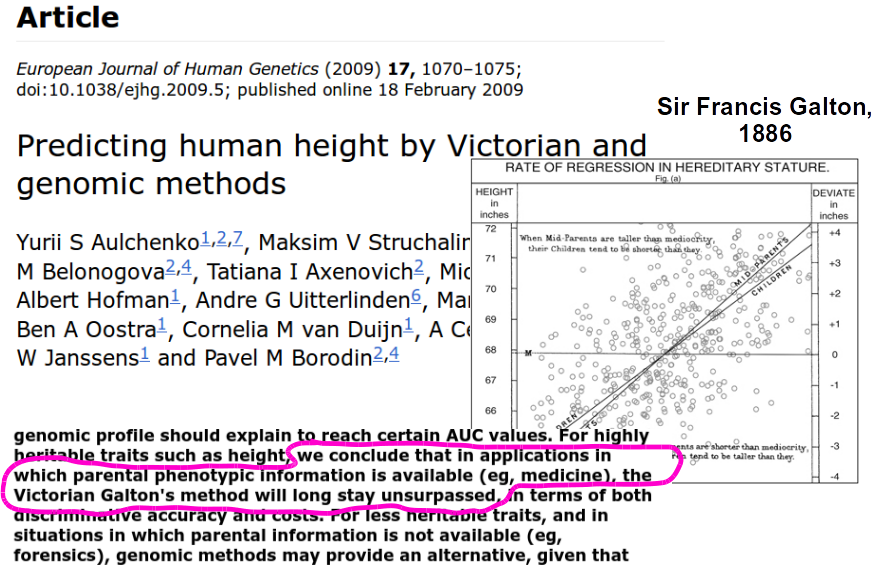
\includegraphics{figures/galton.png}
\caption{Galton Data}
\end{figure}

\begin{itemize}
\tightlist
\item
  The equation takes the form \(\hat{y}=b_0+b_1 * x\)
\item
  The method used to choose the values \(b_0\) and \(b_1\) is to
  minimize the sum of the squares of the residual errors.
\end{itemize}

\subsection{Regression: Galton Data}\label{regression-galton-data}

Not related to Software Engineering but \ldots{}

\begin{Shaded}
\begin{Highlighting}[]
\KeywordTok{library}\NormalTok{(UsingR)}
\KeywordTok{data}\NormalTok{(galton)}
\KeywordTok{par}\NormalTok{(}\DataTypeTok{mfrow=}\KeywordTok{c}\NormalTok{(}\DecValTok{1}\NormalTok{,}\DecValTok{2}\NormalTok{))}
\KeywordTok{hist}\NormalTok{(galton$child,}\DataTypeTok{col=}\StringTok{"blue"}\NormalTok{,}\DataTypeTok{breaks=}\DecValTok{100}\NormalTok{)}
\KeywordTok{hist}\NormalTok{(galton$parent,}\DataTypeTok{col=}\StringTok{"blue"}\NormalTok{,}\DataTypeTok{breaks=}\DecValTok{100}\NormalTok{)}
\end{Highlighting}
\end{Shaded}

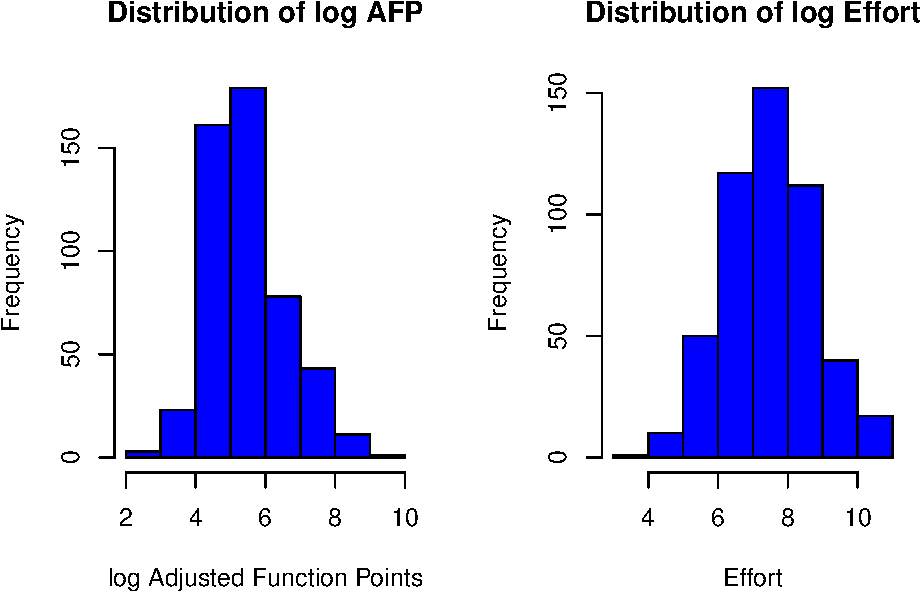
\includegraphics{DASE_files/figure-latex/unnamed-chunk-49-1.pdf}

\begin{Shaded}
\begin{Highlighting}[]
\KeywordTok{plot}\NormalTok{(galton$parent,galton$child,}\DataTypeTok{pch=}\DecValTok{1}\NormalTok{,}\DataTypeTok{col=}\StringTok{"blue"}\NormalTok{, }\DataTypeTok{cex=}\FloatTok{0.4}\NormalTok{)}
\NormalTok{lm1 <-}\StringTok{ }\KeywordTok{lm}\NormalTok{(galton$child ~}\StringTok{ }\NormalTok{galton$parent)}
\KeywordTok{lines}\NormalTok{(galton$parent,lm1$fitted,}\DataTypeTok{col=}\StringTok{"red"}\NormalTok{,}\DataTypeTok{lwd=}\DecValTok{3}\NormalTok{)}
\KeywordTok{plot}\NormalTok{(galton$parent,lm1$residuals,}\DataTypeTok{col=}\StringTok{"blue"}\NormalTok{,}\DataTypeTok{pch=}\DecValTok{1}\NormalTok{, }\DataTypeTok{cex=}\FloatTok{0.4}\NormalTok{)}
\KeywordTok{abline}\NormalTok{(}\KeywordTok{c}\NormalTok{(}\DecValTok{0}\NormalTok{,}\DecValTok{0}\NormalTok{),}\DataTypeTok{col=}\StringTok{"red"}\NormalTok{,}\DataTypeTok{lwd=}\DecValTok{3}\NormalTok{)}
\end{Highlighting}
\end{Shaded}

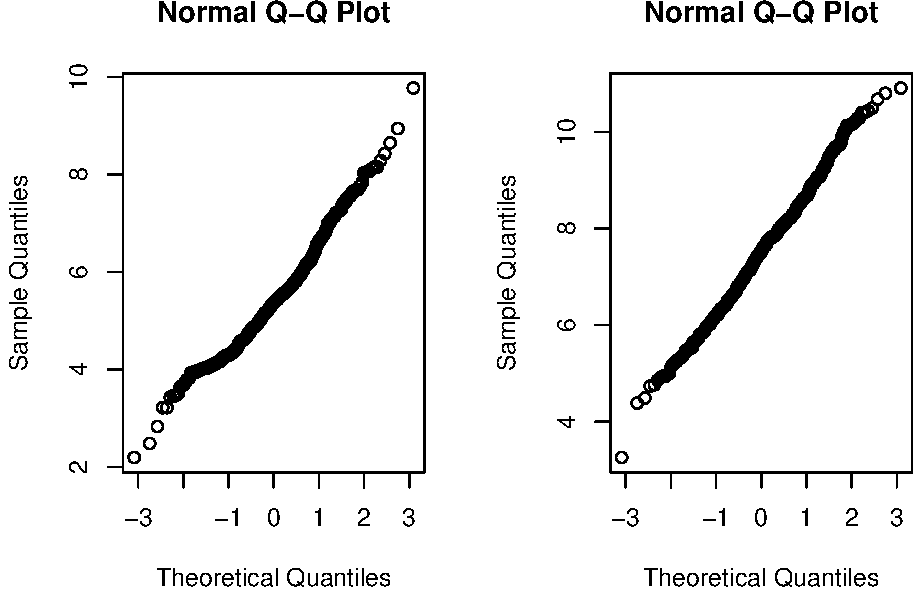
\includegraphics{DASE_files/figure-latex/unnamed-chunk-49-2.pdf}

\begin{Shaded}
\begin{Highlighting}[]
\KeywordTok{qqnorm}\NormalTok{(galton$child)}
\end{Highlighting}
\end{Shaded}

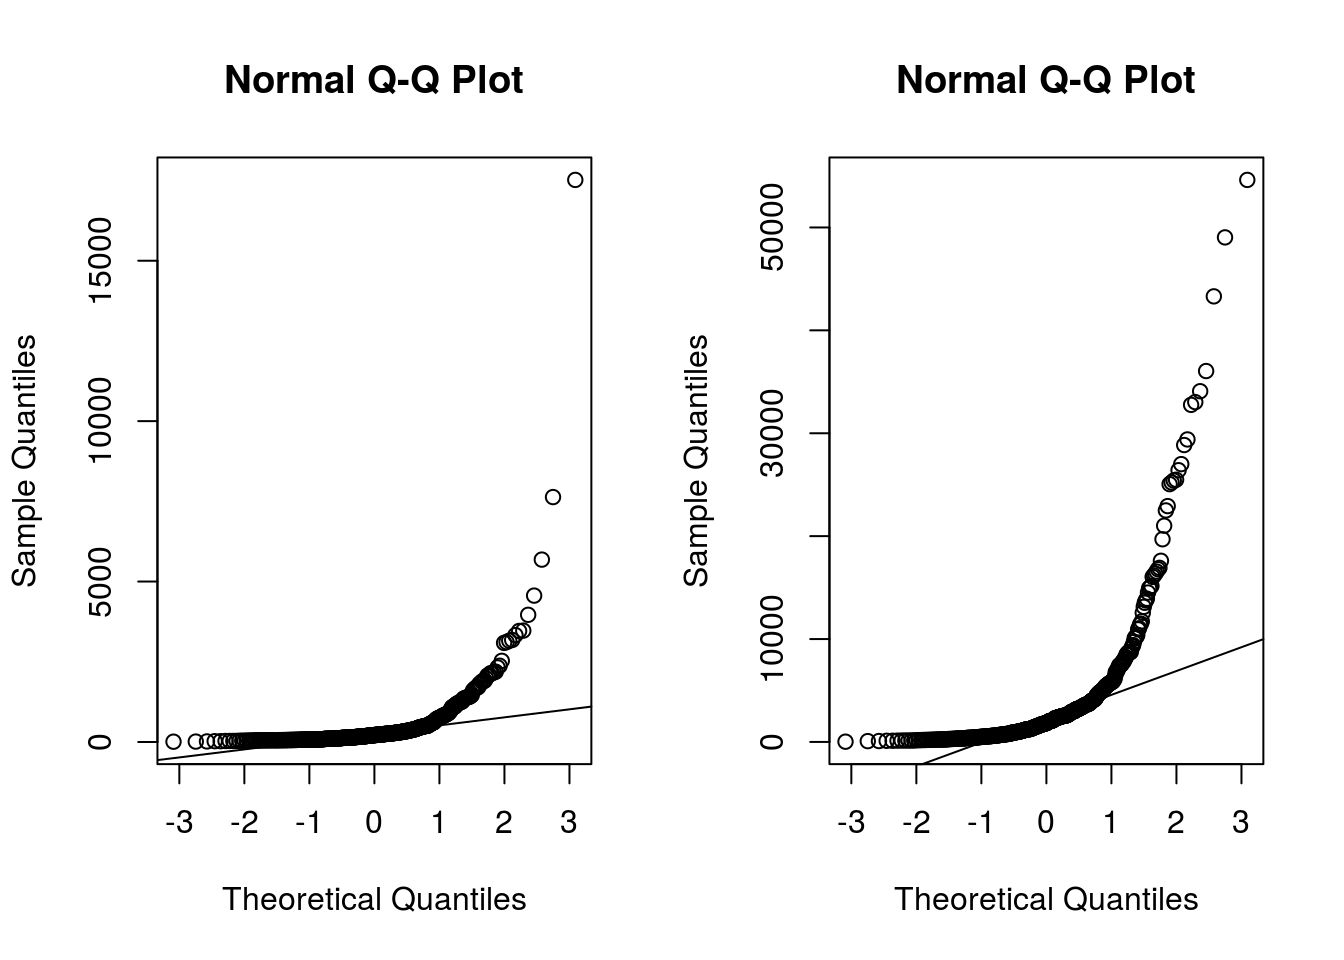
\includegraphics{DASE_files/figure-latex/unnamed-chunk-49-3.pdf}

\subsection{Simple Linear Regression}\label{simple-linear-regression}

\begin{itemize}
\item
  Given two variables \(Y\) (response) and \(X\) (predictor), the
  assumption is that there is an approximate (\(\approx\)) \emph{linear}
  relation between those variables.
\item
  The mathematical model of the observed data is described as (for the
  case of simple linear regression): \[ Y \approx \beta_0 + \beta_1 X\]
\item
  the parameter \(\beta_0\) is named the \emph{intercept} and
  \(\beta_1\) is the \emph{slope}
\item
  Each observation can be modeled as
\end{itemize}

\[y_i = \beta_0 + \beta_1 x_i + \epsilon_i;
\epsilon_i \sim N(0,\sigma^2)\] - \(\epsilon_i\) is the \emph{error} -
This means that the variable \(y\) is normally distributed:
\[ y_i \sim N( \beta_0 + \beta_1 x_i, \sigma^2) \]

\begin{itemize}
\tightlist
\item
  The \emph{predictions} or \emph{estimations} of this model are
  obtained by a linear equation of the form
  \(\hat{Y}=\hat{\beta_0} + \hat{\beta}_1X\), that is, each new
  prediction is computed with
  \[\hat{y}_i = \hat{\beta}_0 + \hat{\beta}_1x_i \].
\item
  The actual parameters \(\beta_0\) and \(\beta_1\) are unknown
\item
  The parameters \(\hat{\beta}_0\) and \(\hat{\beta}_1\) of the linear
  equation can be estimated with different methods.
\end{itemize}

\subsection{Least Squares}\label{least-squares}

\begin{itemize}
\tightlist
\item
  One of the most used methods for computing \(\hat{\beta}_0\) and
  \(\hat{\beta}_1\) is the criterion of ``least squares'' minimization.
\item
  The data is composed of \(n\) pairs of observations \((x_i, y_i)\)
\item
  Given an observation \(y_i\) and its corresponding estimation
  \(\hat{y_i})\) the \emph{residual} \(e_i\) is defined as
  \[e_i= y_i - \hat{y_i}\]
\item
  the Residual Sum of Squares is defined as
  \[RSS=e_1^2+\dots + e_i^2+\dots+e_n^2\]
\item
  the Least Squares Approach minimizes the RSS
\item
  as result of that minimizitation, it can be obtained, by means of
  calculus, the estimation of \(\hat{\beta}_0\) and \(\hat{\beta}_1\) as
  \[\hat{\beta}_1=\frac{\sum_{i=1}^{n}{(x_i-\bar{x})(y_i-\bar{y})}}{\sum_{i=1}^{n}(x_i-\bar{x})^2}\]
  and \[\hat{\beta}_0=\bar{y}-\hat{\beta}_1\bar{x} \] where \(\bar{y}\)
  and \(\bar{x}\) are the sample means.
\item
  the variance \(\sigma^2\) is estimated by
  \[\hat\sigma^2 = {RSS}/{(n-2)}\] where n is the number of observations
\item
  The \emph{Residual Standard Error} is defined as
  \[RSE = \sqrt{{RSS}/{(n-2)}}\]
\item
  The equation \[ Y = \beta_0 + \beta_1 X + \epsilon\] defines the
  linear model, i.e., the \emph{population regression line}
\item
  The \emph{least squares line} is
  \(\hat{Y}=\hat{\beta_0} + \hat{\beta}_1X\)
\item
  \emph{Confidence intervals} are computed using the \emph{standard
  errors} of the intercept and the slope.
\item
  The \(95\%\) confidence interval for the slope is computed as
  \[[\hat{\beta}_1 - 2 \cdot SE(\hat{\beta}_1), \hat{\beta}_1+SE(\hat{\beta}_1)]\]
\item
  where
  \[ SE(\hat{\beta}_1) = \sqrt{\frac{\sigma^2}{\sum_{i=1}^{n}(x_i-\bar{x})^2}}\]
\end{itemize}

\subsection{Linear regression in R}\label{linear-regression-in-r}

The following are the basic commands in R:

\begin{itemize}
\tightlist
\item
  The basic function is \texttt{lm()}, that returns an object with the
  model.
\item
  Other commands: \texttt{summary} prints out information about the
  regression, \texttt{coef} gives the coefficients for the linear model,
  \texttt{fitted} gives the predictd value of \(y\) for each value of
  \(x\), \texttt{residuals} contains the differences between observed
  and fitted values.
\item
  \href{https://stat.ethz.ch/R-manual/R-devel/library/stats/html/predict.lm.html}{\texttt{predict}}
  will generate predicted values of the response for the values of the
  explanatory variable.
\end{itemize}

\section{Linear Regression
Diagnostics}\label{linear-regression-diagnostics}

\begin{itemize}
\tightlist
\item
  Several plots help to evaluate the suitability of the linear
  regression

  \begin{itemize}
  \tightlist
  \item
    \emph{Residuals vs fitted}: The residuals should be randomly
    distributed around the horizontal line representing a residual error
    of zero; that is, there should not be a distinct trend in the
    distribution of points.
  \item
    \emph{Standard Q-Q plot}: residual errors are normally distributed
  \item
    \emph{Square root of the standardized residuals vs the fitted
    values}: there should be no obvious trend. This plot is similar to
    the residuals versus fitted values plot, but it uses the square root
    of the standardized residuals.
  \item
    \emph{Leverage}: measures the importance of each point in
    determining the regression result. Smaller values means that
    removing the observation has little effect on the regression result.
  \end{itemize}
\end{itemize}

\subsection{Simulation example}\label{simulation-example}

\subsubsection{Simulate a dataset}\label{simulate-a-dataset}

\begin{Shaded}
\begin{Highlighting}[]
\KeywordTok{set.seed}\NormalTok{(}\DecValTok{3456}\NormalTok{)}
\CommentTok{# equation is  y = -6.6 + 0.13 x +e}
\CommentTok{# range x 100,400}
\NormalTok{a <-}\StringTok{ }\NormalTok{-}\FloatTok{6.6}
\NormalTok{b <-}\StringTok{ }\FloatTok{0.13}
\NormalTok{num_obs <-}\StringTok{ }\DecValTok{60}
\NormalTok{xmin <-}\StringTok{ }\DecValTok{100}
\NormalTok{xmax <-}\StringTok{ }\DecValTok{400}
\NormalTok{x <-}\StringTok{ }\KeywordTok{sample}\NormalTok{(}\KeywordTok{seq}\NormalTok{(}\DataTypeTok{from=}\NormalTok{xmin, }\DataTypeTok{to =} \NormalTok{xmax, }\DataTypeTok{by =}\DecValTok{1}\NormalTok{), }\DataTypeTok{size=} \NormalTok{num_obs, }\DataTypeTok{replace=}\OtherTok{FALSE}\NormalTok{)}

\NormalTok{sderror <-}\StringTok{ }\DecValTok{9} \CommentTok{# sigma for the error term in the model}
\NormalTok{e <-}\StringTok{ }\KeywordTok{rnorm}\NormalTok{(num_obs, }\DecValTok{0}\NormalTok{, sderror) }

\NormalTok{y <-}\StringTok{ }\NormalTok{a +}\StringTok{ }\NormalTok{b *}\StringTok{ }\NormalTok{x +}\StringTok{ }\NormalTok{e}


\NormalTok{newlm <-}\StringTok{ }\KeywordTok{lm}\NormalTok{(y~x)}
\KeywordTok{summary}\NormalTok{(newlm)}
\end{Highlighting}
\end{Shaded}

\begin{verbatim}
## 
## Call:
## lm(formula = y ~ x)
## 
## Residuals:
##     Min      1Q  Median      3Q     Max 
## -15.937  -4.617  -0.923   3.797  21.442 
## 
## Coefficients:
##             Estimate Std. Error t value Pr(>|t|)    
## (Intercept) -13.4765     3.0320   -4.44    4e-05 ***
## x             0.1550     0.0113   13.75   <2e-16 ***
## ---
## Signif. codes:  0 '***' 0.001 '**' 0.01 '*' 0.05 '.' 0.1 ' ' 1
## 
## Residual standard error: 7.99 on 58 degrees of freedom
## Multiple R-squared:  0.765,  Adjusted R-squared:  0.761 
## F-statistic:  189 on 1 and 58 DF,  p-value: <2e-16
\end{verbatim}

\begin{Shaded}
\begin{Highlighting}[]
\NormalTok{cfa1 <-}\StringTok{ }\KeywordTok{coef}\NormalTok{(newlm)[}\DecValTok{1}\NormalTok{]}
\NormalTok{cfb2 <-}\StringTok{ }\KeywordTok{coef}\NormalTok{(newlm)[}\DecValTok{2}\NormalTok{]}
\KeywordTok{plot}\NormalTok{(x,y, }\DataTypeTok{xlab=}\StringTok{"x axis"}\NormalTok{, }\DataTypeTok{ylab=} \StringTok{"y axis"}\NormalTok{, }\DataTypeTok{xlim =} \KeywordTok{c}\NormalTok{(xmin, xmax), }\DataTypeTok{ylim =} \KeywordTok{c}\NormalTok{(}\DecValTok{0}\NormalTok{,}\DecValTok{60}\NormalTok{), }\DataTypeTok{sub =} \StringTok{"Line in black is the actual model"}\NormalTok{)}
\KeywordTok{title}\NormalTok{(}\DataTypeTok{main =} \KeywordTok{paste}\NormalTok{(}\StringTok{"Line in blue is the Regression Line for "}\NormalTok{, num_obs, }\StringTok{" points."}\NormalTok{))}

\KeywordTok{abline}\NormalTok{(}\DataTypeTok{a =} \NormalTok{cfa1, }\DataTypeTok{b =} \NormalTok{cfb2, }\DataTypeTok{col=} \StringTok{"blue"}\NormalTok{, }\DataTypeTok{lwd=}\DecValTok{3}\NormalTok{)}
\KeywordTok{abline}\NormalTok{(}\DataTypeTok{a =} \NormalTok{a, }\DataTypeTok{b =} \NormalTok{b, }\DataTypeTok{col=} \StringTok{"black"}\NormalTok{, }\DataTypeTok{lwd=}\DecValTok{1}\NormalTok{) }\CommentTok{#original line}
\end{Highlighting}
\end{Shaded}

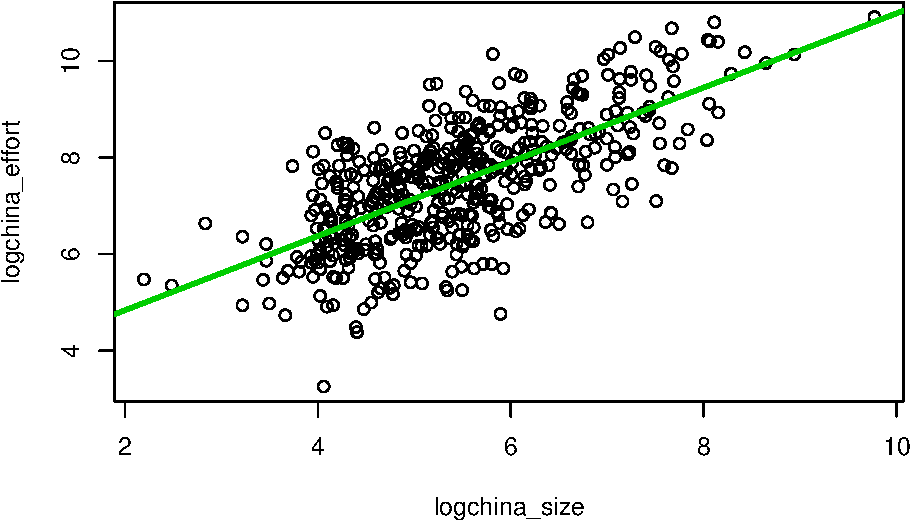
\includegraphics{DASE_files/figure-latex/unnamed-chunk-50-1.pdf}

\paragraph{Subset a set of points from the same
sample}\label{subset-a-set-of-points-from-the-same-sample}

\begin{Shaded}
\begin{Highlighting}[]
\CommentTok{# sample from  the same  x     to compare least squares lines }
\CommentTok{# change the denominator in newsample to see how the least square lines changes accordingly. }
\NormalTok{newsample <-}\StringTok{ }\KeywordTok{as.integer}\NormalTok{(num_obs/}\DecValTok{8}\NormalTok{) }\CommentTok{# number of pairs x,y}

\NormalTok{idxs_x1 <-}\StringTok{ }\KeywordTok{sample}\NormalTok{(}\DecValTok{1}\NormalTok{:num_obs, }\DataTypeTok{size =} \NormalTok{newsample, }\DataTypeTok{replace =} \OtherTok{FALSE}\NormalTok{) }\CommentTok{#sample indexes}
\NormalTok{x1 <-}\StringTok{ }\NormalTok{x[idxs_x1]}
\NormalTok{e1 <-}\StringTok{ }\NormalTok{e[idxs_x1]}
\NormalTok{y1 <-}\StringTok{ }\NormalTok{a +}\StringTok{ }\NormalTok{b *}\StringTok{ }\NormalTok{x1 +}\StringTok{ }\NormalTok{e1}
\NormalTok{xy_obs <-}\StringTok{ }\KeywordTok{data.frame}\NormalTok{(x1, y1)}
\KeywordTok{names}\NormalTok{(xy_obs) <-}\StringTok{ }\KeywordTok{c}\NormalTok{(}\StringTok{"x_obs"}\NormalTok{, }\StringTok{"y_obs"}\NormalTok{)}

\NormalTok{newlm1 <-}\StringTok{ }\KeywordTok{lm}\NormalTok{(y1~x1)}
\KeywordTok{summary}\NormalTok{(newlm1)}
\end{Highlighting}
\end{Shaded}

\begin{verbatim}
## 
## Call:
## lm(formula = y1 ~ x1)
## 
## Residuals:
##      1      2      3      4      5      6      7 
##  3.722 -5.067  4.683 -4.716  3.095 -0.813 -0.904 
## 
## Coefficients:
##             Estimate Std. Error t value Pr(>|t|)   
## (Intercept) -14.5356     7.0962   -2.05   0.0958 . 
## x1            0.1494     0.0272    5.48   0.0027 **
## ---
## Signif. codes:  0 '***' 0.001 '**' 0.01 '*' 0.05 '.' 0.1 ' ' 1
## 
## Residual standard error: 4.35 on 5 degrees of freedom
## Multiple R-squared:  0.857,  Adjusted R-squared:  0.829 
## F-statistic: 30.1 on 1 and 5 DF,  p-value: 0.00275
\end{verbatim}

\begin{Shaded}
\begin{Highlighting}[]
\NormalTok{cfa21 <-}\StringTok{ }\KeywordTok{coef}\NormalTok{(newlm1)[}\DecValTok{1}\NormalTok{]}
\NormalTok{cfb22 <-}\StringTok{ }\KeywordTok{coef}\NormalTok{(newlm1)[}\DecValTok{2}\NormalTok{]}

\KeywordTok{plot}\NormalTok{(x1,y1, }\DataTypeTok{xlab=}\StringTok{"x axis"}\NormalTok{, }\DataTypeTok{ylab=} \StringTok{"y axis"}\NormalTok{, }\DataTypeTok{xlim =} \KeywordTok{c}\NormalTok{(xmin, xmax), }\DataTypeTok{ylim =} \KeywordTok{c}\NormalTok{(}\DecValTok{0}\NormalTok{,}\DecValTok{60}\NormalTok{))}
\KeywordTok{title}\NormalTok{(}\DataTypeTok{main =} \KeywordTok{paste}\NormalTok{(}\StringTok{"New line in red with "}\NormalTok{, newsample, }\StringTok{" points in sample"}\NormalTok{))}

\KeywordTok{abline}\NormalTok{(}\DataTypeTok{a =} \NormalTok{a, }\DataTypeTok{b =} \NormalTok{b, }\DataTypeTok{col=} \StringTok{"black"}\NormalTok{, }\DataTypeTok{lwd=}\DecValTok{1}\NormalTok{)  }\CommentTok{# True line}
\KeywordTok{abline}\NormalTok{(}\DataTypeTok{a =} \NormalTok{cfa1, }\DataTypeTok{b =} \NormalTok{cfb2, }\DataTypeTok{col=} \StringTok{"blue"}\NormalTok{, }\DataTypeTok{lwd=}\DecValTok{1}\NormalTok{)  }\CommentTok{#sample}
\KeywordTok{abline}\NormalTok{(}\DataTypeTok{a =} \NormalTok{cfa21, }\DataTypeTok{b =} \NormalTok{cfb22, }\DataTypeTok{col=} \StringTok{"red"}\NormalTok{, }\DataTypeTok{lwd=}\DecValTok{2}\NormalTok{) }\CommentTok{#new line}
\end{Highlighting}
\end{Shaded}

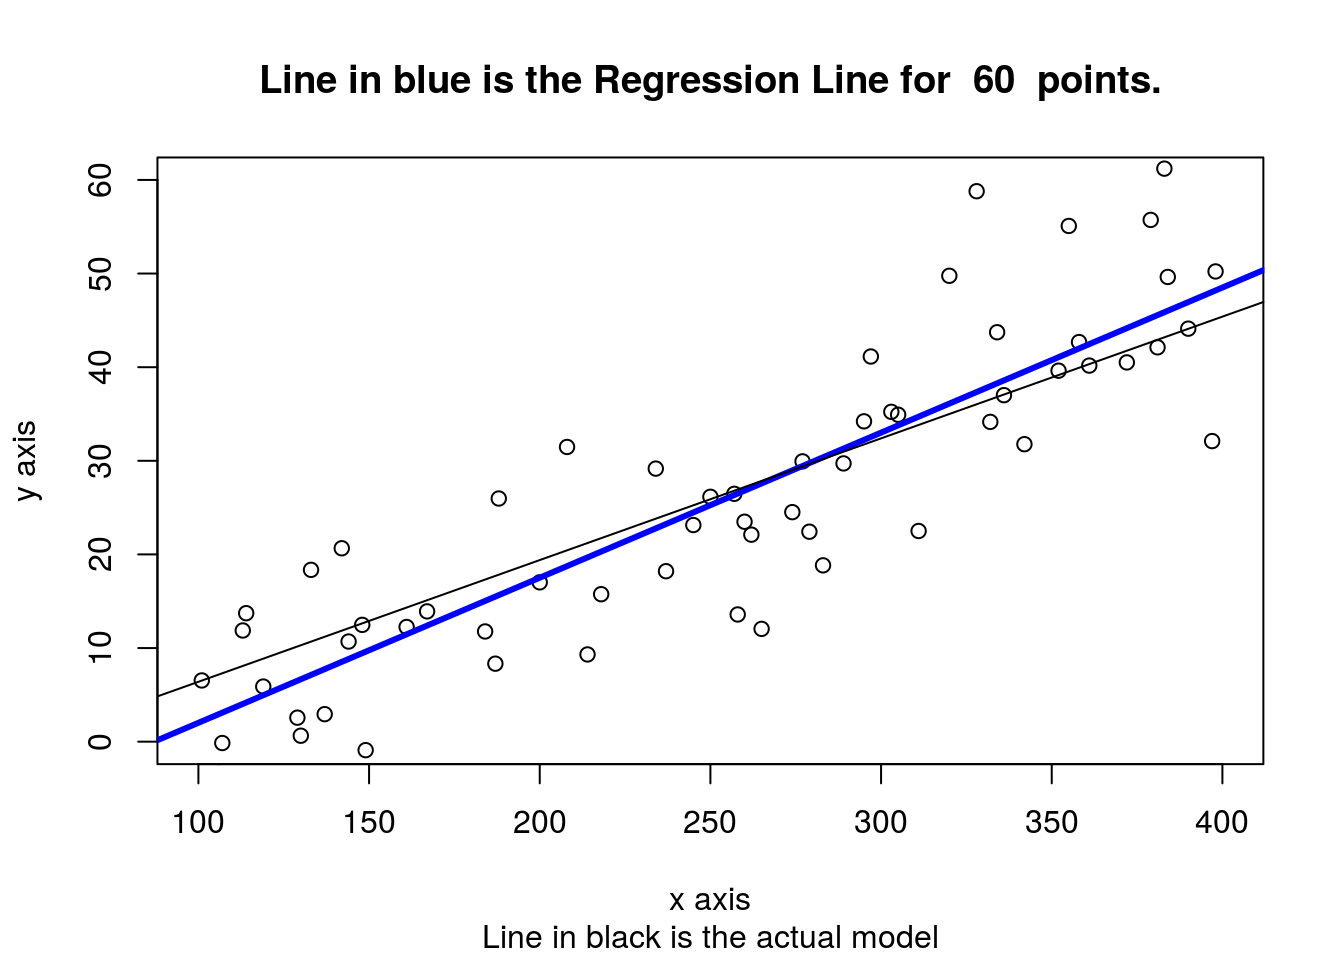
\includegraphics{DASE_files/figure-latex/unnamed-chunk-51-1.pdf}

\paragraph{Compute a confidence interval on the original sample
regression
line}\label{compute-a-confidence-interval-on-the-original-sample-regression-line}

\begin{Shaded}
\begin{Highlighting}[]
\NormalTok{newx <-}\StringTok{ }\KeywordTok{seq}\NormalTok{(xmin, xmax)}
\NormalTok{ypredicted <-}\StringTok{ }\KeywordTok{predict}\NormalTok{(newlm, }\DataTypeTok{newdata=}\KeywordTok{data.frame}\NormalTok{(}\DataTypeTok{x=}\NormalTok{newx), }\DataTypeTok{interval=} \StringTok{"confidence"}\NormalTok{, }\DataTypeTok{level=} \FloatTok{0.90}\NormalTok{, }\DataTypeTok{se =} \OtherTok{TRUE}\NormalTok{)}

\KeywordTok{plot}\NormalTok{(x,y, }\DataTypeTok{xlab=}\StringTok{"x axis"}\NormalTok{, }\DataTypeTok{ylab=} \StringTok{"y axis"}\NormalTok{, }\DataTypeTok{xlim =} \KeywordTok{c}\NormalTok{(xmin, xmax), }\DataTypeTok{ylim =} \KeywordTok{c}\NormalTok{(}\DecValTok{0}\NormalTok{,}\DecValTok{60}\NormalTok{))}
\CommentTok{# points(x1, fitted(newlm1))}
\KeywordTok{abline}\NormalTok{(newlm)}

\KeywordTok{lines}\NormalTok{(newx,ypredicted$fit[,}\DecValTok{2}\NormalTok{],}\DataTypeTok{col=}\StringTok{"red"}\NormalTok{,}\DataTypeTok{lty=}\DecValTok{2}\NormalTok{)}
\KeywordTok{lines}\NormalTok{(newx,ypredicted$fit[,}\DecValTok{3}\NormalTok{],}\DataTypeTok{col=}\StringTok{"red"}\NormalTok{,}\DataTypeTok{lty=}\DecValTok{2}\NormalTok{)}
\end{Highlighting}
\end{Shaded}

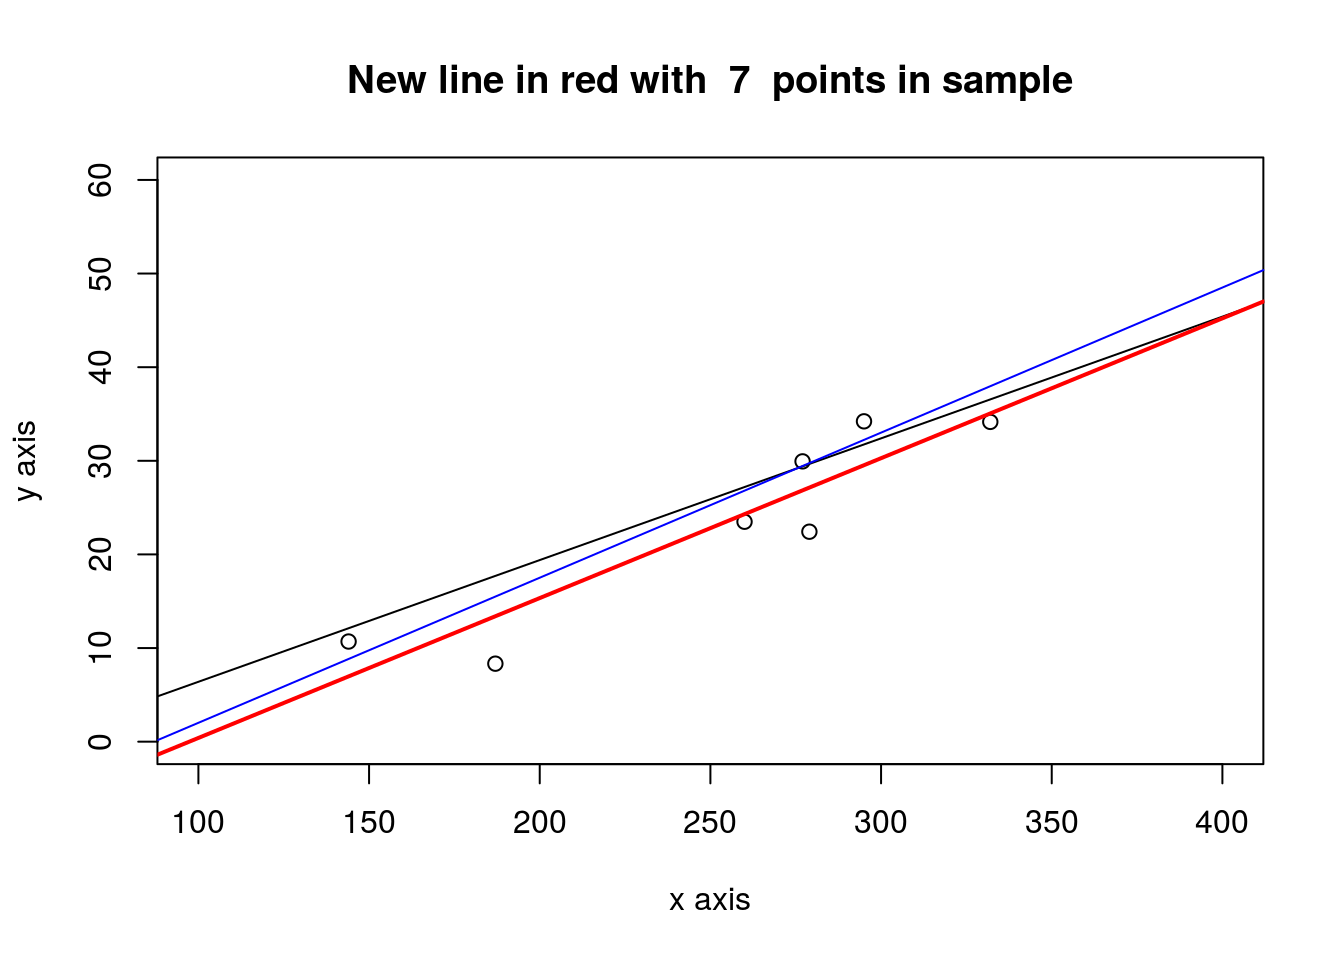
\includegraphics{DASE_files/figure-latex/unnamed-chunk-52-1.pdf}

\begin{Shaded}
\begin{Highlighting}[]
\CommentTok{# Plot the residuals or errors}
\NormalTok{ypredicted_x <-}\StringTok{ }\KeywordTok{predict}\NormalTok{(newlm, }\DataTypeTok{newdata=}\KeywordTok{data.frame}\NormalTok{(}\DataTypeTok{x=}\NormalTok{x))}
\KeywordTok{plot}\NormalTok{(x,y, }\DataTypeTok{xlab=}\StringTok{"x axis"}\NormalTok{, }\DataTypeTok{ylab=} \StringTok{"y axis"}\NormalTok{, }\DataTypeTok{xlim =} \KeywordTok{c}\NormalTok{(xmin, xmax), }\DataTypeTok{ylim =} \KeywordTok{c}\NormalTok{(}\DecValTok{0}\NormalTok{,}\DecValTok{60}\NormalTok{), }\DataTypeTok{sub =} \StringTok{""}\NormalTok{, }\DataTypeTok{pch=}\DecValTok{19}\NormalTok{, }\DataTypeTok{cex=}\FloatTok{0.75}\NormalTok{)}
\KeywordTok{title}\NormalTok{(}\DataTypeTok{main =} \KeywordTok{paste}\NormalTok{(}\StringTok{"Residuals or errors"}\NormalTok{, num_obs, }\StringTok{" points."}\NormalTok{))}
\KeywordTok{abline}\NormalTok{(newlm)}
\KeywordTok{segments}\NormalTok{(x, y, x, ypredicted_x)}
\end{Highlighting}
\end{Shaded}

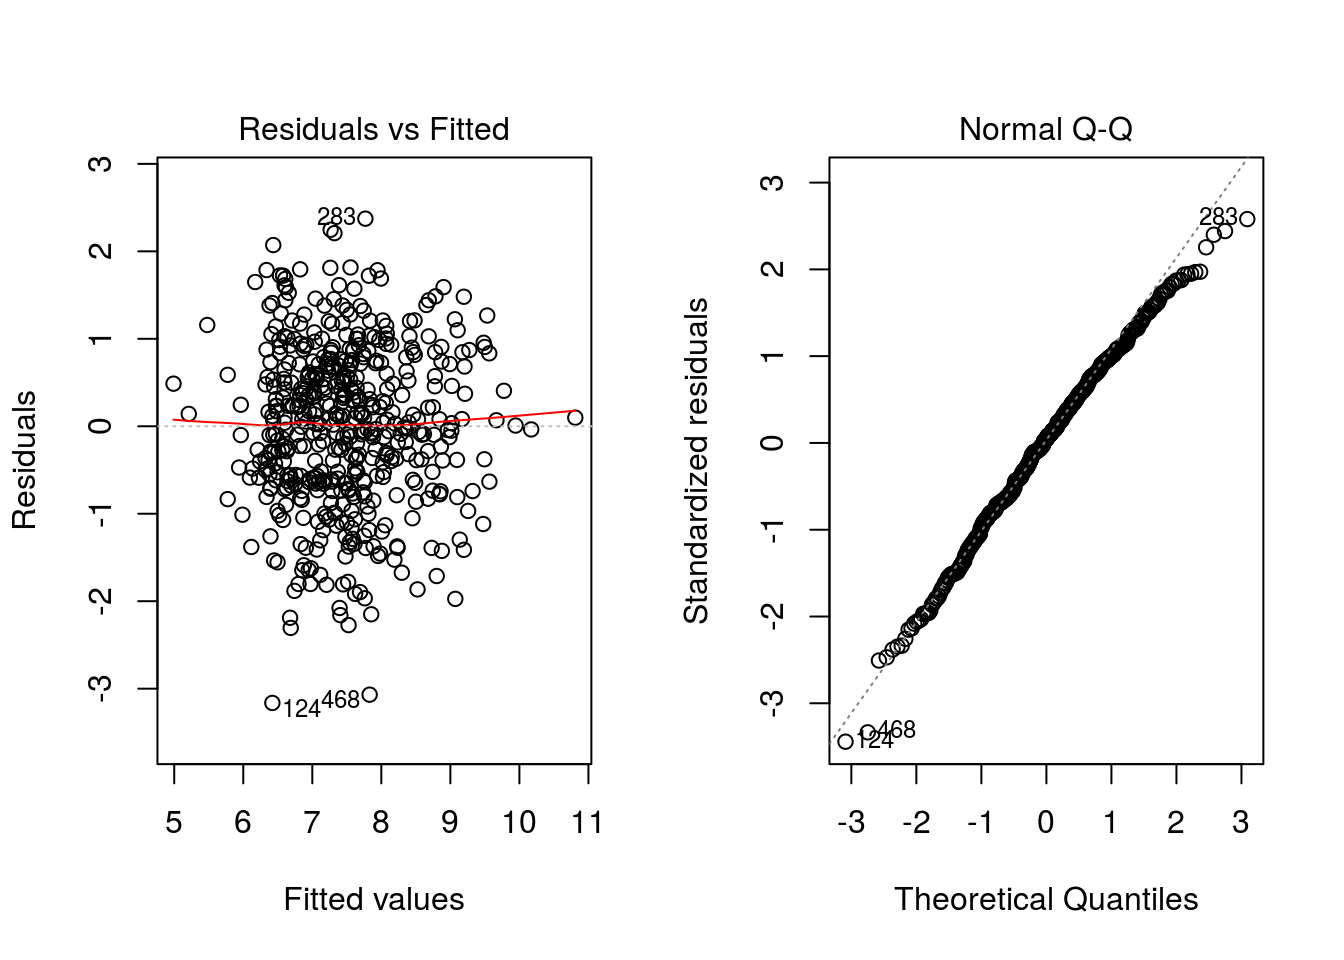
\includegraphics{DASE_files/figure-latex/unnamed-chunk-52-2.pdf}

\paragraph{Take another sample from the model and
explore}\label{take-another-sample-from-the-model-and-explore}

\begin{Shaded}
\begin{Highlighting}[]
\CommentTok{# equation is  y = -6.6 + 0.13 x +e}
\CommentTok{# range x 100,400}
\NormalTok{num_obs <-}\StringTok{ }\DecValTok{35}
\NormalTok{xmin <-}\StringTok{ }\DecValTok{100}
\NormalTok{xmax <-}\StringTok{ }\DecValTok{400}
\NormalTok{x3 <-}\StringTok{ }\KeywordTok{sample}\NormalTok{(}\KeywordTok{seq}\NormalTok{(}\DataTypeTok{from=}\NormalTok{xmin, }\DataTypeTok{to =} \NormalTok{xmax, }\DataTypeTok{by =}\DecValTok{1}\NormalTok{), }\DataTypeTok{size=} \NormalTok{num_obs, }\DataTypeTok{replace=}\OtherTok{FALSE}\NormalTok{)}
\NormalTok{sderror <-}\StringTok{ }\DecValTok{14} \CommentTok{# sigma for the error term in the model}
\NormalTok{e3 <-}\StringTok{ }\KeywordTok{rnorm}\NormalTok{(num_obs, }\DecValTok{0}\NormalTok{, sderror) }

\NormalTok{y3 <-}\StringTok{ }\NormalTok{a +}\StringTok{ }\NormalTok{b *}\StringTok{ }\NormalTok{x3 +}\StringTok{ }\NormalTok{e3}

\NormalTok{newlm3 <-}\StringTok{ }\KeywordTok{lm}\NormalTok{(y3~x3)}
\KeywordTok{summary}\NormalTok{(newlm3)}
\end{Highlighting}
\end{Shaded}

\begin{verbatim}
## 
## Call:
## lm(formula = y3 ~ x3)
## 
## Residuals:
##    Min     1Q Median     3Q    Max 
## -25.59 -11.19   2.92   8.65  39.16 
## 
## Coefficients:
##             Estimate Std. Error t value Pr(>|t|)    
## (Intercept) -17.5335     7.6813   -2.28    0.029 *  
## x3            0.1657     0.0285    5.80  1.7e-06 ***
## ---
## Signif. codes:  0 '***' 0.001 '**' 0.01 '*' 0.05 '.' 0.1 ' ' 1
## 
## Residual standard error: 15 on 33 degrees of freedom
## Multiple R-squared:  0.505,  Adjusted R-squared:  0.49 
## F-statistic: 33.7 on 1 and 33 DF,  p-value: 1.72e-06
\end{verbatim}

\begin{Shaded}
\begin{Highlighting}[]
\NormalTok{cfa31 <-}\StringTok{ }\KeywordTok{coef}\NormalTok{(newlm3)[}\DecValTok{1}\NormalTok{]}
\NormalTok{cfb32 <-}\StringTok{ }\KeywordTok{coef}\NormalTok{(newlm3)[}\DecValTok{2}\NormalTok{]}
\KeywordTok{plot}\NormalTok{(x3,y3, }\DataTypeTok{xlab=}\StringTok{"x axis"}\NormalTok{, }\DataTypeTok{ylab=} \StringTok{"y axis"}\NormalTok{, }\DataTypeTok{xlim =} \KeywordTok{c}\NormalTok{(xmin, xmax), }\DataTypeTok{ylim =} \KeywordTok{c}\NormalTok{(}\DecValTok{0}\NormalTok{,}\DecValTok{60}\NormalTok{))}
\KeywordTok{title}\NormalTok{(}\DataTypeTok{main =} \KeywordTok{paste}\NormalTok{(}\StringTok{"Line in red is the Regression Line for "}\NormalTok{, num_obs, }\StringTok{" points."}\NormalTok{))}
\KeywordTok{abline}\NormalTok{(}\DataTypeTok{a =} \NormalTok{cfa31, }\DataTypeTok{b =} \NormalTok{cfb32, }\DataTypeTok{col=} \StringTok{"red"}\NormalTok{, }\DataTypeTok{lwd=}\DecValTok{3}\NormalTok{)}
\KeywordTok{abline}\NormalTok{(}\DataTypeTok{a =} \NormalTok{a, }\DataTypeTok{b =} \NormalTok{b, }\DataTypeTok{col=} \StringTok{"black"}\NormalTok{, }\DataTypeTok{lwd=}\DecValTok{2}\NormalTok{) }\CommentTok{#original line}
\KeywordTok{abline}\NormalTok{(}\DataTypeTok{a =} \NormalTok{cfa1, }\DataTypeTok{b =} \NormalTok{cfb2, }\DataTypeTok{col=} \StringTok{"blue"}\NormalTok{, }\DataTypeTok{lwd=}\DecValTok{1}\NormalTok{) }\CommentTok{#first sample}

\CommentTok{# confidence intervals for the new sample}

\NormalTok{newx <-}\StringTok{ }\KeywordTok{seq}\NormalTok{(xmin, xmax)}
\NormalTok{ypredicted <-}\StringTok{ }\KeywordTok{predict}\NormalTok{(newlm3, }\DataTypeTok{newdata=}\KeywordTok{data.frame}\NormalTok{(}\DataTypeTok{x3=}\NormalTok{newx), }\DataTypeTok{interval=} \StringTok{"confidence"}\NormalTok{, }\DataTypeTok{level=} \FloatTok{0.90}\NormalTok{, }\DataTypeTok{se =} \OtherTok{TRUE}\NormalTok{)}

\KeywordTok{lines}\NormalTok{(newx,ypredicted$fit[,}\DecValTok{2}\NormalTok{],}\DataTypeTok{col=}\StringTok{"red"}\NormalTok{,}\DataTypeTok{lty=}\DecValTok{2}\NormalTok{, }\DataTypeTok{lwd=}\DecValTok{2}\NormalTok{)}
\KeywordTok{lines}\NormalTok{(newx,ypredicted$fit[,}\DecValTok{3}\NormalTok{],}\DataTypeTok{col=}\StringTok{"red"}\NormalTok{,}\DataTypeTok{lty=}\DecValTok{2}\NormalTok{, }\DataTypeTok{lwd=}\DecValTok{2}\NormalTok{)}
\end{Highlighting}
\end{Shaded}

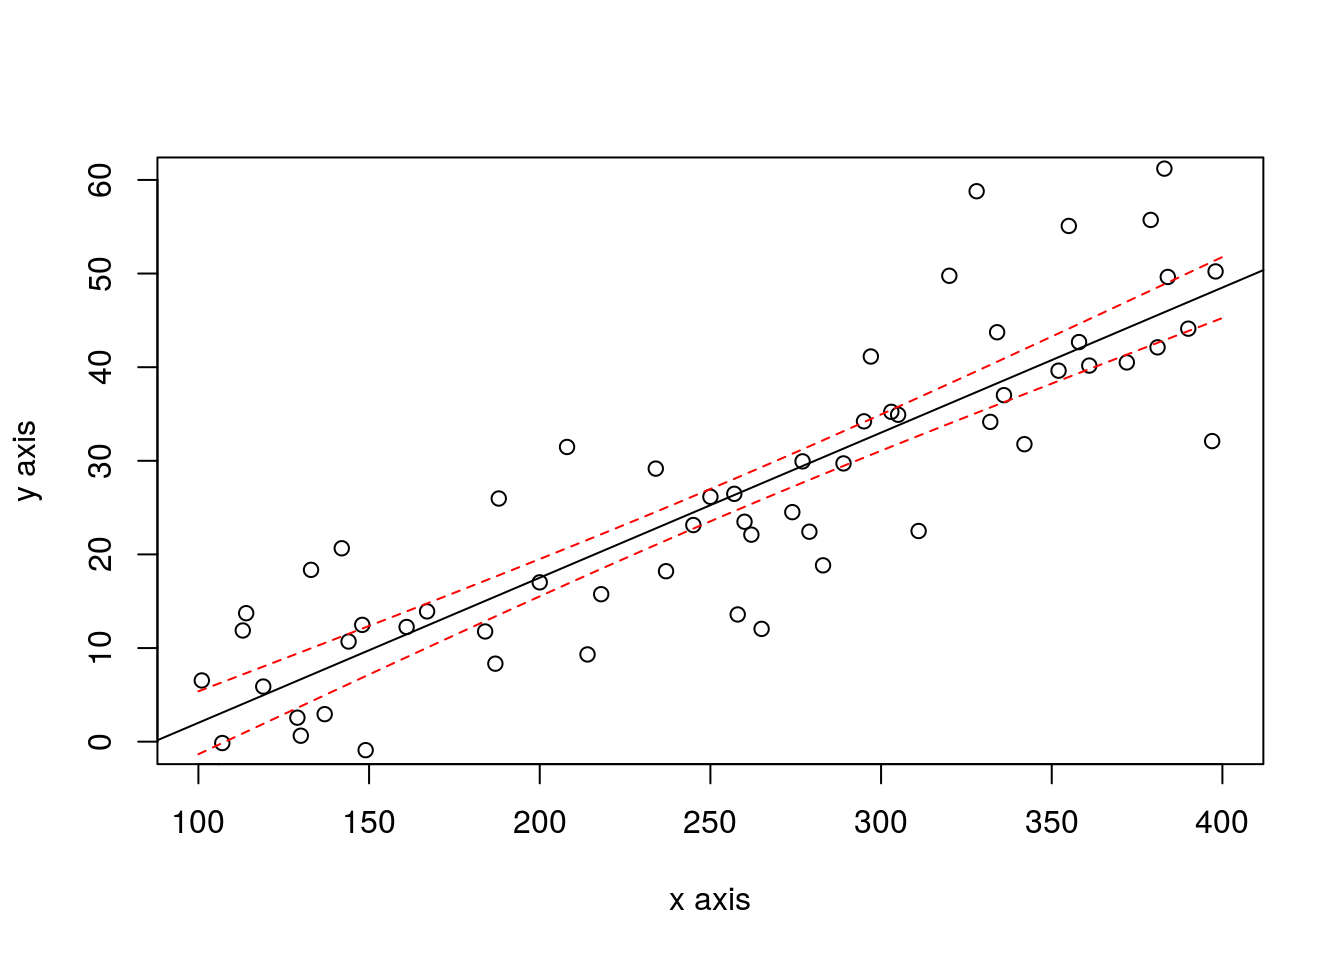
\includegraphics{DASE_files/figure-latex/unnamed-chunk-53-1.pdf}

\subsection{Diagnostics fro assessing the regression
line}\label{diagnostics-fro-assessing-the-regression-line}

\subsubsection{Residual Standard Error}\label{residual-standard-error}

\begin{itemize}
\tightlist
\item
  It gives us an idea of the typical or average error of the model. It
  is the estimated standard deviation of the residuals.
\end{itemize}

\subsubsection{\texorpdfstring{\(R^2\)
statistic}{R\^{}2 statistic}}\label{r2-statistic}

\begin{itemize}
\tightlist
\item
  This is the proportion of variability in the data that is explained by
  the model. Best values are those close to 1.
\end{itemize}

\section{Multiple Linear Regression}\label{multiple-linear-regression}

\subsection{Partial Least Squares}\label{partial-least-squares}

\begin{itemize}
\tightlist
\item
  If several predictors are highly correlated, the least squares
  approach has high variability.
\item
  PLS finds linear combinations of the predictors, that are called
  \emph{components} or \emph{latent} variables.
\end{itemize}

\section{Linear regression in Software Effort
estimation}\label{linear-regression-in-software-effort-estimation}

Fitting a linear model to log-log - the predictive power equation is
\(y= e^{b_0 + b_1 log(x)}\), ignoring the bias corrections - First, we
are fitting the model to the whole dataset. But it is not the right way
to do it, because of overfitting.

\begin{Shaded}
\begin{Highlighting}[]
\KeywordTok{library}\NormalTok{(foreign)}
\NormalTok{china <-}\StringTok{ }\KeywordTok{read.arff}\NormalTok{(}\StringTok{"./datasets/effortEstimation/china.arff"}\NormalTok{)}
\NormalTok{china_size <-}\StringTok{ }\NormalTok{china$AFP}
\KeywordTok{summary}\NormalTok{(china_size)}
\end{Highlighting}
\end{Shaded}

\begin{verbatim}
##    Min. 1st Qu.  Median    Mean 3rd Qu.    Max. 
##       9     100     215     487     438   17500
\end{verbatim}

\begin{Shaded}
\begin{Highlighting}[]
\NormalTok{china_effort <-}\StringTok{ }\NormalTok{china$Effort}
\KeywordTok{summary}\NormalTok{(china_effort)}
\end{Highlighting}
\end{Shaded}

\begin{verbatim}
##    Min. 1st Qu.  Median    Mean 3rd Qu.    Max. 
##      26     704    1830    3920    3830   54600
\end{verbatim}

\begin{Shaded}
\begin{Highlighting}[]
\KeywordTok{par}\NormalTok{(}\DataTypeTok{mfrow=}\KeywordTok{c}\NormalTok{(}\DecValTok{1}\NormalTok{,}\DecValTok{2}\NormalTok{))}
\KeywordTok{hist}\NormalTok{(china_size, }\DataTypeTok{col=}\StringTok{"blue"}\NormalTok{, }\DataTypeTok{xlab=}\StringTok{"Adjusted Function Points"}\NormalTok{, }\DataTypeTok{main=}\StringTok{"Distribution of AFP"}\NormalTok{)}
\KeywordTok{hist}\NormalTok{(china_effort, }\DataTypeTok{col=}\StringTok{"blue"}\NormalTok{,}\DataTypeTok{xlab=}\StringTok{"Effort"}\NormalTok{, }\DataTypeTok{main=}\StringTok{"Distribution of Effort"}\NormalTok{)}
\end{Highlighting}
\end{Shaded}

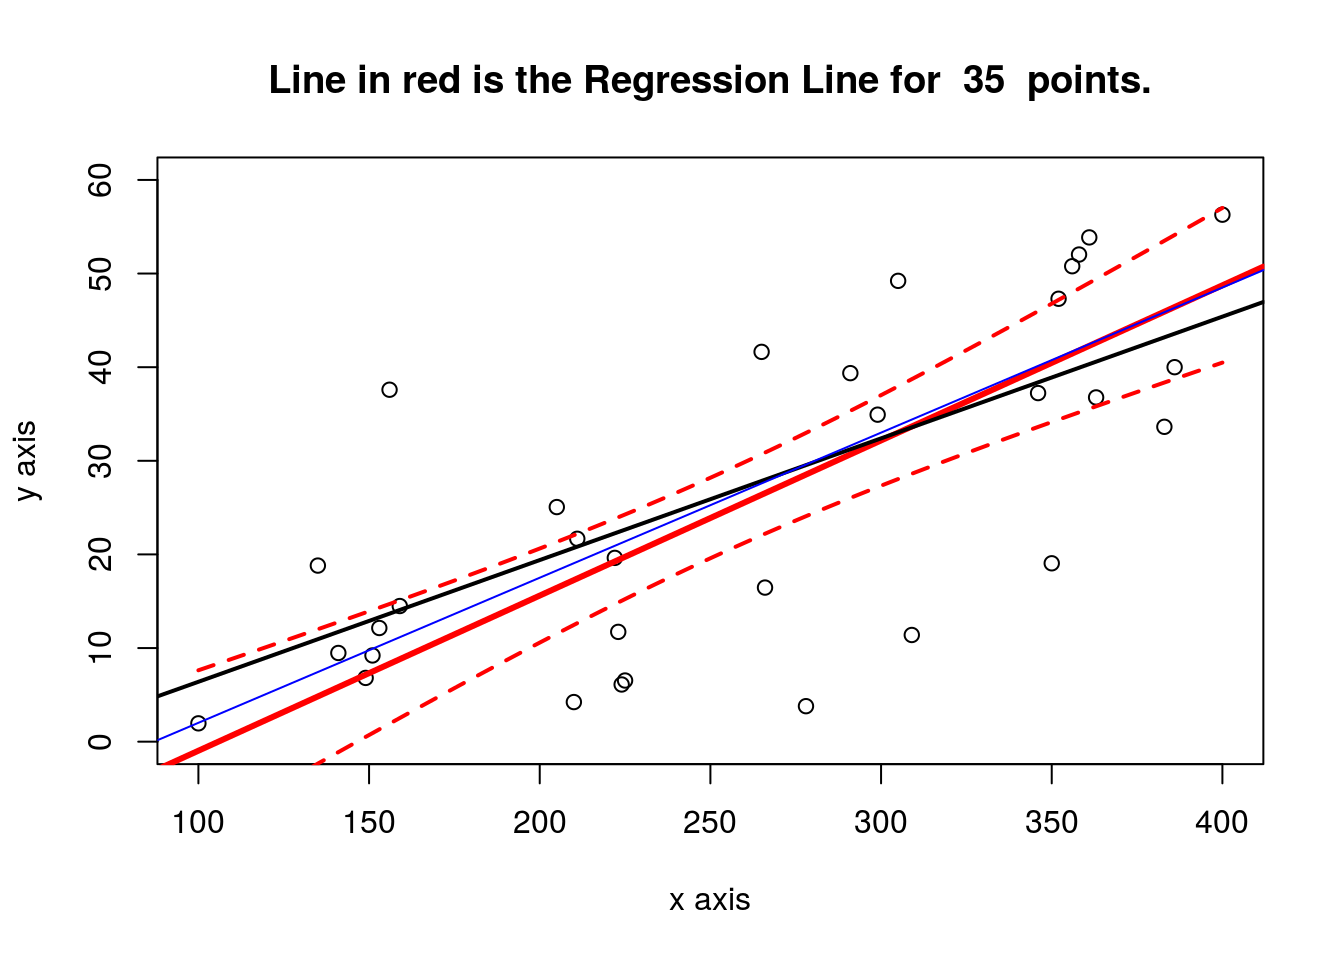
\includegraphics{DASE_files/figure-latex/unnamed-chunk-54-1.pdf}

\begin{Shaded}
\begin{Highlighting}[]
\KeywordTok{boxplot}\NormalTok{(china_size)}
\KeywordTok{boxplot}\NormalTok{(china_effort)}
\end{Highlighting}
\end{Shaded}

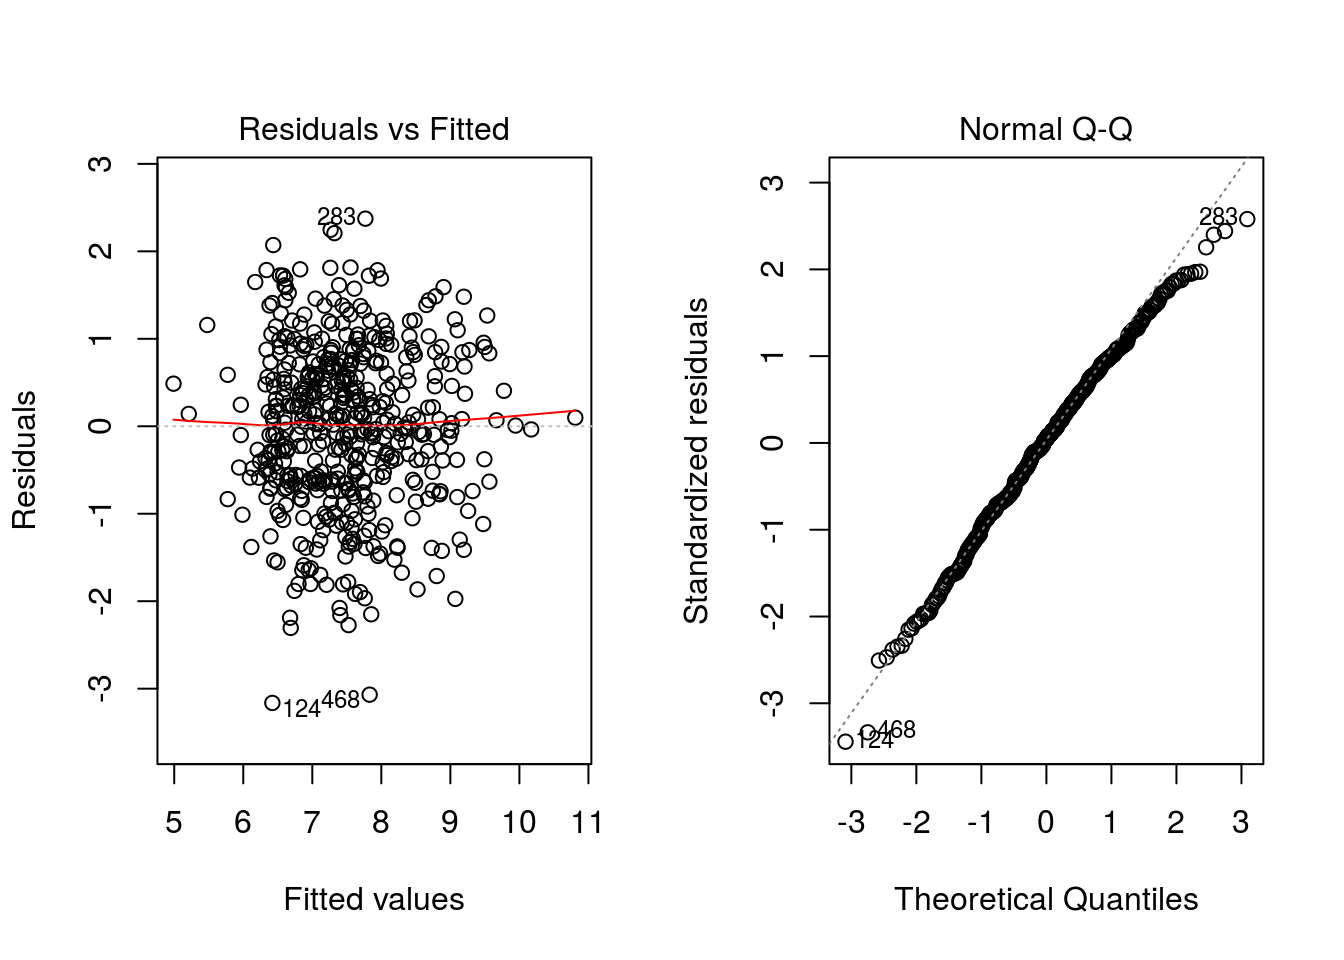
\includegraphics{DASE_files/figure-latex/unnamed-chunk-54-2.pdf}

\begin{Shaded}
\begin{Highlighting}[]
\KeywordTok{qqnorm}\NormalTok{(china_size)}
\KeywordTok{qqline}\NormalTok{(china_size)}
\KeywordTok{qqnorm}\NormalTok{(china_effort)}
\KeywordTok{qqline}\NormalTok{(china_effort)}
\end{Highlighting}
\end{Shaded}

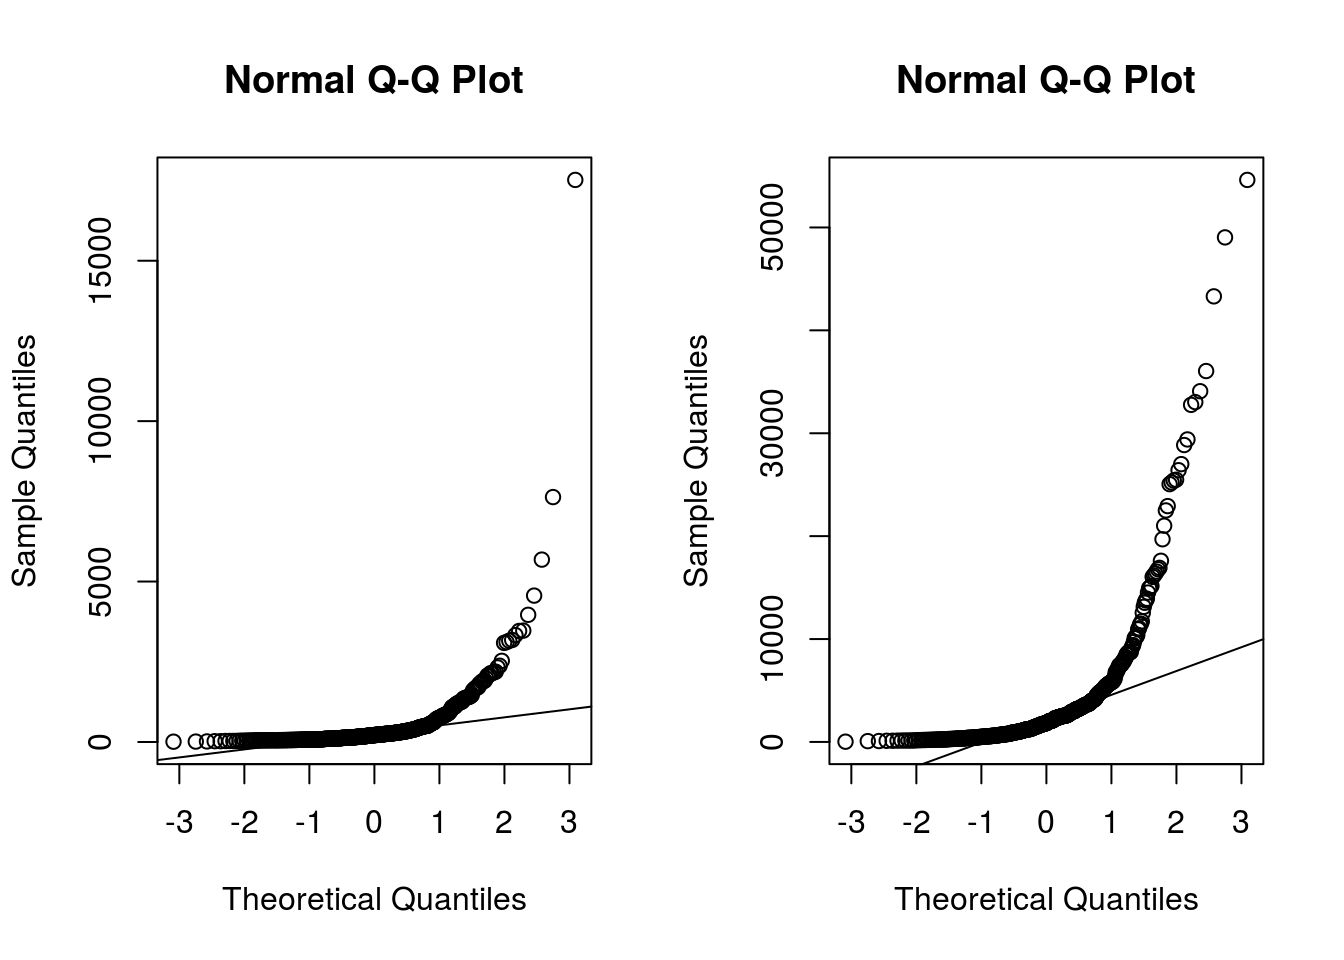
\includegraphics{DASE_files/figure-latex/unnamed-chunk-54-3.pdf}

Applying the \texttt{log} function

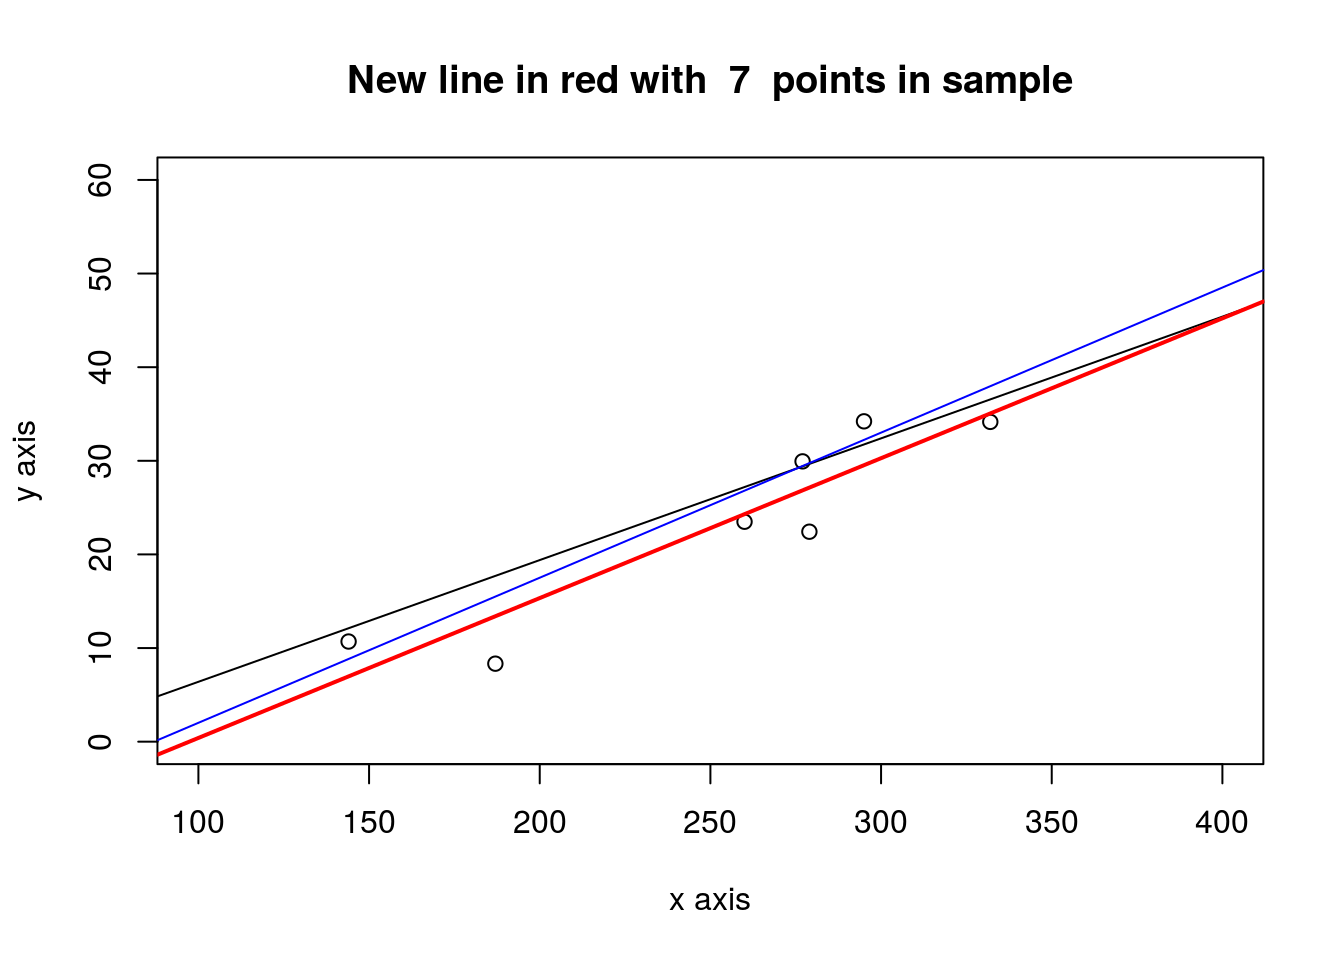
\includegraphics{DASE_files/figure-latex/unnamed-chunk-55-1.pdf}
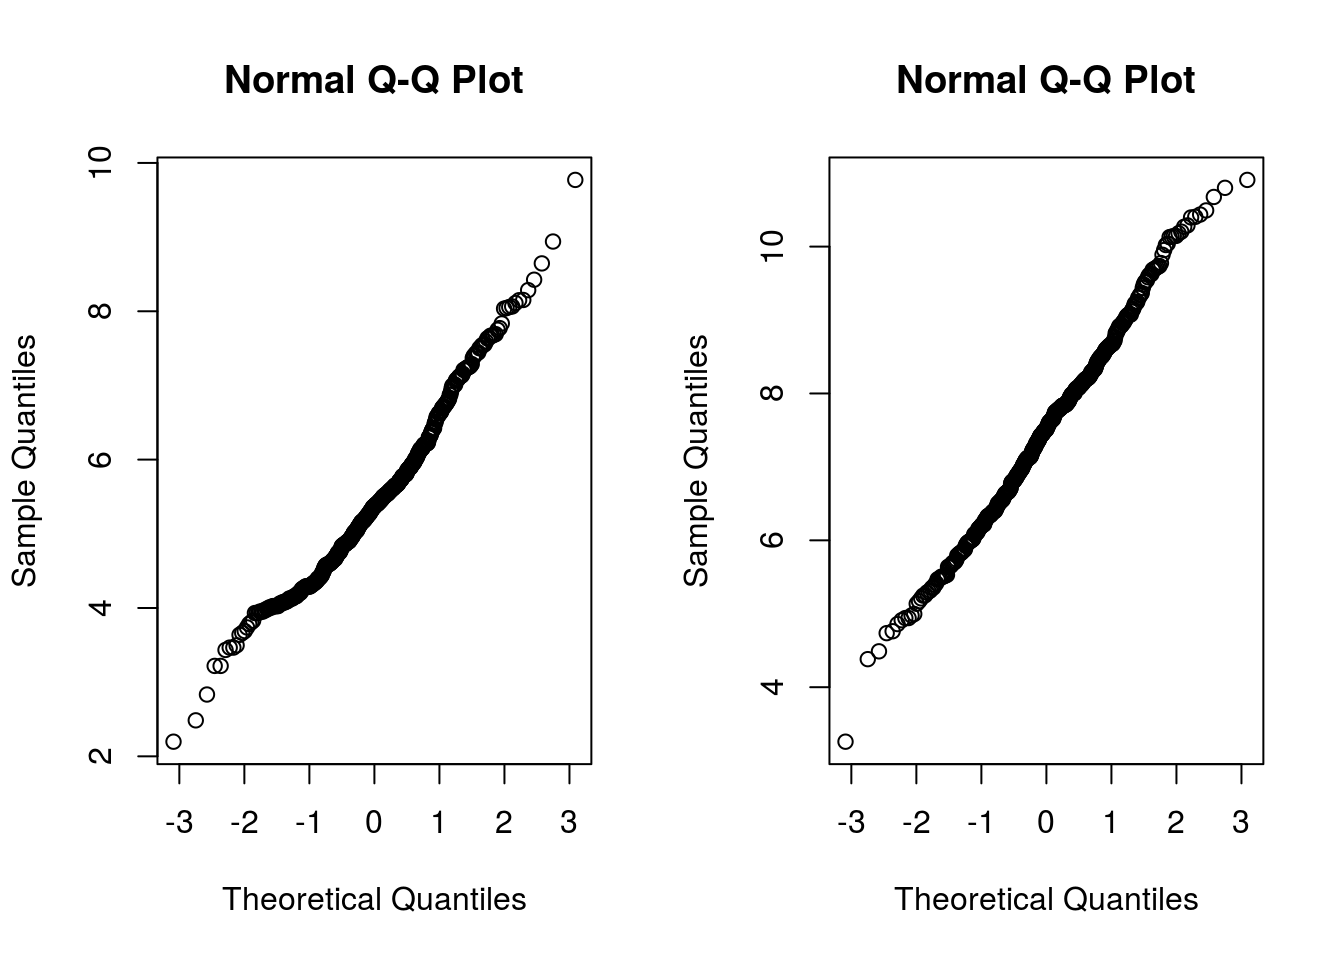
\includegraphics{DASE_files/figure-latex/unnamed-chunk-55-2.pdf}

\begin{Shaded}
\begin{Highlighting}[]
\NormalTok{linmodel_logchina <-}\StringTok{ }\KeywordTok{lm}\NormalTok{(logchina_effort ~}\StringTok{ }\NormalTok{logchina_size)}
\KeywordTok{par}\NormalTok{(}\DataTypeTok{mfrow=}\KeywordTok{c}\NormalTok{(}\DecValTok{1}\NormalTok{,}\DecValTok{1}\NormalTok{))}
\KeywordTok{plot}\NormalTok{(logchina_size, logchina_effort)}
\KeywordTok{abline}\NormalTok{(linmodel_logchina, }\DataTypeTok{lwd=}\DecValTok{3}\NormalTok{, }\DataTypeTok{col=}\DecValTok{3}\NormalTok{)}
\end{Highlighting}
\end{Shaded}

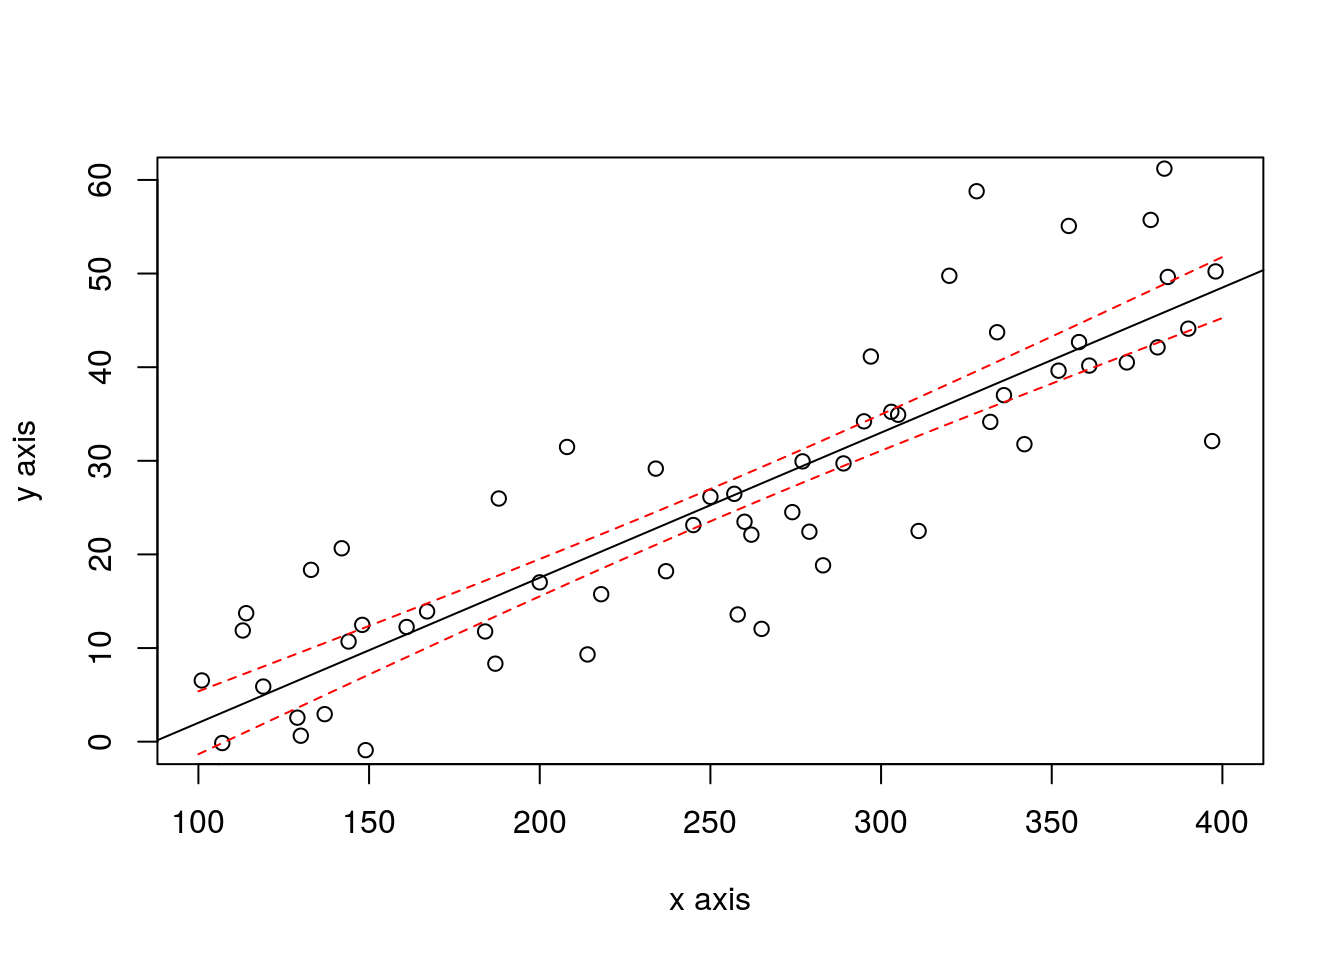
\includegraphics{DASE_files/figure-latex/unnamed-chunk-56-1.pdf}

\begin{Shaded}
\begin{Highlighting}[]
\KeywordTok{par}\NormalTok{(}\DataTypeTok{mfrow=}\KeywordTok{c}\NormalTok{(}\DecValTok{1}\NormalTok{,}\DecValTok{2}\NormalTok{))}
\KeywordTok{plot}\NormalTok{(linmodel_logchina, }\DataTypeTok{ask =} \OtherTok{FALSE}\NormalTok{)}
\end{Highlighting}
\end{Shaded}

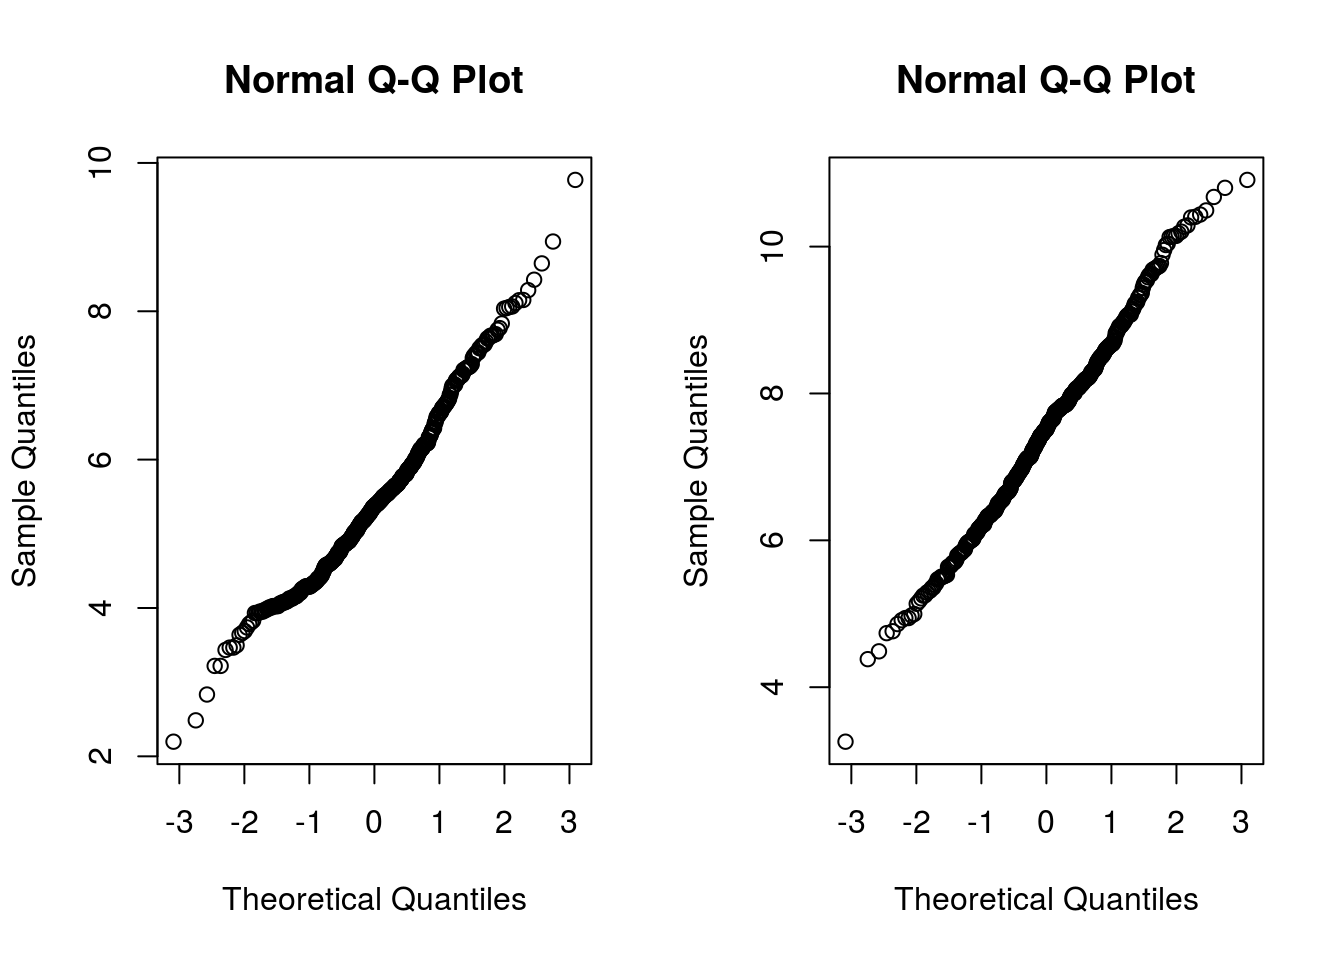
\includegraphics{DASE_files/figure-latex/unnamed-chunk-56-2.pdf}
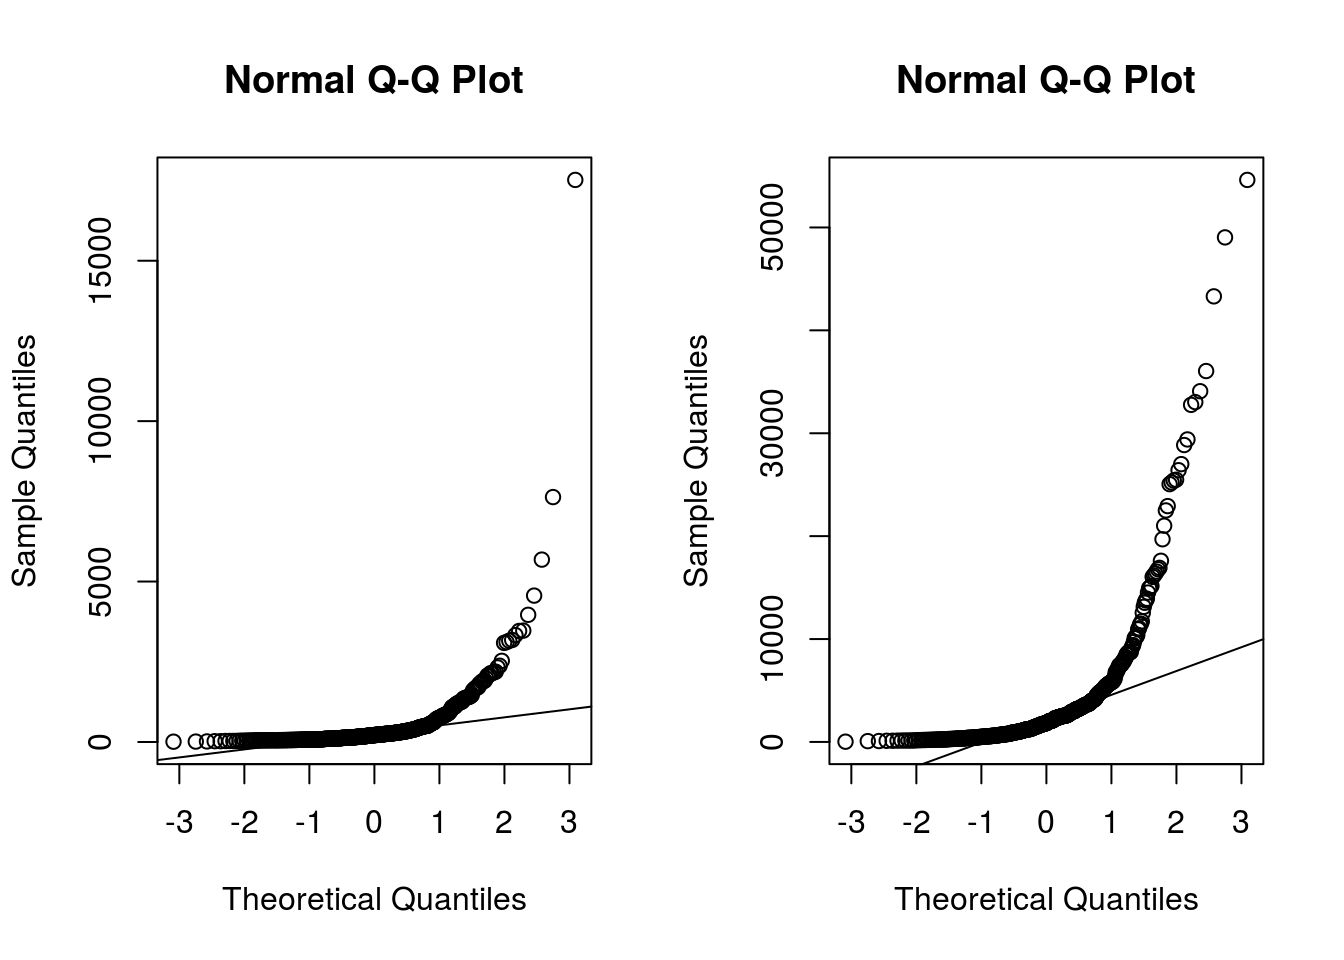
\includegraphics{DASE_files/figure-latex/unnamed-chunk-56-3.pdf}

\begin{Shaded}
\begin{Highlighting}[]
\NormalTok{linmodel_logchina}
\end{Highlighting}
\end{Shaded}

\begin{verbatim}
## 
## Call:
## lm(formula = logchina_effort ~ logchina_size)
## 
## Coefficients:
##   (Intercept)  logchina_size  
##         3.301          0.768
\end{verbatim}

\section{References}\label{references}

\begin{itemize}
\tightlist
\item
  The New Statistics with R, Andy Hector, 2015
\item
  An Introduction to R, W.N. Venables and D.M. Smith and the R
  Development Core Team
\item
  Practical Data Science with R, Nina Zumel and John Mount
\item
  G. James et al, An Introduction to Statistical Learning with
  Applications in R, Springer, 2013
\end{itemize}

\chapter{Discrete Classification}\label{discrete-classification}

We also have several types of models such as trees, rules, and
probabilistic classifiers that can be used to classify instances in
There are many p

We will show the use of different classification techniques in the
problem of defect prediction as running example. In this example, the
different datasets are composed of classical metrics (Halstead or McCabe
metrics) based on counts of operators/operands and like or
object-oriented metrics (e.g.~Chidamber and Kemerer) and the class
attribute indicating whether the module or class was defective.

\section{The caret package}\label{the-caret-package}

There are hundreds of packages to perform classification task in R, but
many of those can be used throught the `caret' package which helps with
many of the data mining process task as described next.

The \href{http://topepo.github.io/caret/}{caret (Classification And
REgression Training) package} provides a unified interface for modeling
and prediction with around 150 different models with tools for:

\begin{verbatim}
+ data splitting
+ pre-processing
+ feature selection
+ model tuning using resampling
+ variable importance estimation, etc.
\end{verbatim}

Website: \url{http://caret.r-forge.r-project.org}

JSS Paper: \url{www.jstatsoft.org/v28/i05/paper}

Book: \href{http://AppliedPredictiveModeling.com/}{Applied Predictive
Modeling}

For example, using one of the NASA datasets used extensively in defect
prediction:

\begin{Shaded}
\begin{Highlighting}[]
\KeywordTok{library}\NormalTok{(caret)}
\KeywordTok{library}\NormalTok{(foreign)}

\NormalTok{kc1 <-}\StringTok{ }\KeywordTok{read.arff}\NormalTok{(}\StringTok{"./datasets/defectPred/D1/KC1.arff"}\NormalTok{)}
\KeywordTok{str}\NormalTok{(kc1)}
\end{Highlighting}
\end{Shaded}

\begin{verbatim}
## 'data.frame':    2096 obs. of  22 variables:
##  $ LOC_BLANK            : num  0 0 0 0 2 0 0 0 0 2 ...
##  $ BRANCH_COUNT         : num  1 1 1 1 1 1 1 1 1 1 ...
##  $ LOC_CODE_AND_COMMENT : num  0 0 0 0 0 0 0 0 0 0 ...
##  $ LOC_COMMENTS         : num  0 0 0 0 0 0 0 0 0 0 ...
##  $ CYCLOMATIC_COMPLEXITY: num  1 1 1 1 1 1 1 1 1 1 ...
##  $ DESIGN_COMPLEXITY    : num  1 1 1 1 1 1 1 1 1 1 ...
##  $ ESSENTIAL_COMPLEXITY : num  1 1 1 1 1 1 1 1 1 1 ...
##  $ LOC_EXECUTABLE       : num  3 1 1 1 8 3 1 1 1 9 ...
##  $ HALSTEAD_CONTENT     : num  11.6 0 0 0 18 ...
##  $ HALSTEAD_DIFFICULTY  : num  2.67 0 0 0 3.5 2.67 0 0 0 3.75 ...
##  $ HALSTEAD_EFFORT      : num  82.3 0 0 0 220.9 ...
##  $ HALSTEAD_ERROR_EST   : num  0.01 0 0 0 0.02 0.01 0 0 0 0.04 ...
##  $ HALSTEAD_LENGTH      : num  11 1 1 1 19 11 1 1 1 29 ...
##  $ HALSTEAD_LEVEL       : num  0.38 0 0 0 0.29 0.38 0 0 0 0.27 ...
##  $ HALSTEAD_PROG_TIME   : num  4.57 0 0 0 12.27 ...
##  $ HALSTEAD_VOLUME      : num  30.9 0 0 0 63.1 ...
##  $ NUM_OPERANDS         : num  4 0 0 0 7 4 0 0 0 10 ...
##  $ NUM_OPERATORS        : num  7 1 1 1 12 7 1 1 1 19 ...
##  $ NUM_UNIQUE_OPERANDS  : num  3 0 0 0 5 3 0 0 0 8 ...
##  $ NUM_UNIQUE_OPERATORS : num  4 1 1 1 5 4 1 1 1 6 ...
##  $ LOC_TOTAL            : num  5 3 3 3 12 5 3 3 3 13 ...
##  $ Defective            : Factor w/ 2 levels "N","Y": 1 1 1 1 1 1 1 1 1 1 ...
\end{verbatim}

Then we need to divide the data into training and testing.

\begin{Shaded}
\begin{Highlighting}[]
\CommentTok{# Split data into training and test datasets}
\KeywordTok{set.seed}\NormalTok{(}\DecValTok{1}\NormalTok{)}
\NormalTok{inTrain <-}\StringTok{ }\KeywordTok{createDataPartition}\NormalTok{(}\DataTypeTok{y=}\NormalTok{kc1$Defective,}\DataTypeTok{p=}\NormalTok{.}\DecValTok{75}\NormalTok{,}\DataTypeTok{list=}\OtherTok{FALSE}\NormalTok{)}
\NormalTok{kc1.train <-}\StringTok{ }\NormalTok{kc1[inTrain,]}
\NormalTok{kc1.test <-}\StringTok{ }\NormalTok{kc1[-inTrain,]}
\end{Highlighting}
\end{Shaded}

Another approach to dividing the data:

\begin{Shaded}
\begin{Highlighting}[]
\CommentTok{# Split data into training and test datasets}

\KeywordTok{set.seed}\NormalTok{(}\DecValTok{1}\NormalTok{)}
\NormalTok{ind <-}\StringTok{ }\KeywordTok{sample}\NormalTok{(}\DecValTok{2}\NormalTok{, }\KeywordTok{nrow}\NormalTok{(kc1), }\DataTypeTok{replace =} \OtherTok{TRUE}\NormalTok{, }\DataTypeTok{prob =} \KeywordTok{c}\NormalTok{(}\FloatTok{0.75}\NormalTok{, }\FloatTok{0.25}\NormalTok{))}
\NormalTok{kc1.train <-}\StringTok{ }\NormalTok{kc1[ind==}\DecValTok{1}\NormalTok{, ]}
\NormalTok{kc1.test <-}\StringTok{ }\NormalTok{kc1[ind==}\DecValTok{2}\NormalTok{, ]}
\end{Highlighting}
\end{Shaded}

Next we will use different types of models to predict defective modules.

\section{Linear Discriminant Analysis
(LDA)}\label{linear-discriminant-analysis-lda}

One classical approach to classification is Linear Discriminant Analysis
(LDA).

\begin{Shaded}
\begin{Highlighting}[]
\NormalTok{ldaModel <-}\StringTok{ }\KeywordTok{train} \NormalTok{(Defective ~}\StringTok{ }\NormalTok{., }\DataTypeTok{data=}\NormalTok{kc1.train, }\DataTypeTok{method=}\StringTok{"lda"}\NormalTok{, }\DataTypeTok{preProc=}\KeywordTok{c}\NormalTok{(}\StringTok{"center"}\NormalTok{,}\StringTok{"scale"}\NormalTok{))}

\NormalTok{ldaModel}
\end{Highlighting}
\end{Shaded}

\begin{verbatim}
## Linear Discriminant Analysis 
## 
## 1573 samples
##   21 predictors
##    2 classes: 'N', 'Y' 
## 
## Pre-processing: centered (21), scaled (21) 
## Resampling: Bootstrapped (25 reps) 
## Summary of sample sizes: 1573, 1573, 1573, 1573, 1573, 1573, ... 
## Resampling results:
## 
##   Accuracy  Kappa
##   0.855     0.286
## 
## 
\end{verbatim}

We can observe that we are training our model using
\texttt{Defective\ \textasciitilde{}\ .} as a formula were 'Defective is
the class variable separed by \texttt{\textasciitilde{}} and the ´.´
means the rest of the variables. Also, we are using a filter for the
training data to (preProc) to center and scale.

Also, as stated in the documentation about the \texttt{train} method :
\textgreater{} \url{http://topepo.github.io/caret/training.html}

\begin{Shaded}
\begin{Highlighting}[]
\NormalTok{ctrl <-}\StringTok{ }\KeywordTok{trainControl}\NormalTok{(}\DataTypeTok{method =} \StringTok{"repeatedcv"}\NormalTok{,}\DataTypeTok{repeats=}\DecValTok{3}\NormalTok{)}
\NormalTok{ldaModel <-}\StringTok{ }\KeywordTok{train} \NormalTok{(Defective ~}\StringTok{ }\NormalTok{., }\DataTypeTok{data=}\NormalTok{kc1.train, }\DataTypeTok{method=}\StringTok{"lda"}\NormalTok{, }\DataTypeTok{trControl=}\NormalTok{ctrl, }\DataTypeTok{preProc=}\KeywordTok{c}\NormalTok{(}\StringTok{"center"}\NormalTok{,}\StringTok{"scale"}\NormalTok{))}

\NormalTok{ldaModel}
\end{Highlighting}
\end{Shaded}

\begin{verbatim}
## Linear Discriminant Analysis 
## 
## 1573 samples
##   21 predictors
##    2 classes: 'N', 'Y' 
## 
## Pre-processing: centered (21), scaled (21) 
## Resampling: Cross-Validated (10 fold, repeated 3 times) 
## Summary of sample sizes: 1416, 1416, 1415, 1416, 1415, 1416, ... 
## Resampling results:
## 
##   Accuracy  Kappa
##   0.854     0.288
## 
## 
\end{verbatim}

Instead of accuracy we can activate other metrics using
\texttt{summaryFunction=twoClassSummary} such as \texttt{ROC},
\texttt{sensitivity} and \texttt{specificity}. To do so, we also need to
speficy \texttt{classProbs=TRUE}.

\begin{Shaded}
\begin{Highlighting}[]
\NormalTok{ctrl <-}\StringTok{ }\KeywordTok{trainControl}\NormalTok{(}\DataTypeTok{method =} \StringTok{"repeatedcv"}\NormalTok{,}\DataTypeTok{repeats=}\DecValTok{3}\NormalTok{, }\DataTypeTok{classProbs=}\OtherTok{TRUE}\NormalTok{,}
\DataTypeTok{summaryFunction=}\NormalTok{twoClassSummary)}
\NormalTok{ldaModel3xcv10 <-}\StringTok{ }\KeywordTok{train} \NormalTok{(Defective ~}\StringTok{ }\NormalTok{., }\DataTypeTok{data=}\NormalTok{kc1.train, }\DataTypeTok{method=}\StringTok{"lda"}\NormalTok{, }\DataTypeTok{trControl=}\NormalTok{ctrl, }\DataTypeTok{preProc=}\KeywordTok{c}\NormalTok{(}\StringTok{"center"}\NormalTok{,}\StringTok{"scale"}\NormalTok{))}

\NormalTok{ldaModel3xcv10}
\end{Highlighting}
\end{Shaded}

\begin{verbatim}
## Linear Discriminant Analysis 
## 
## 1573 samples
##   21 predictors
##    2 classes: 'N', 'Y' 
## 
## Pre-processing: centered (21), scaled (21) 
## Resampling: Cross-Validated (10 fold, repeated 3 times) 
## Summary of sample sizes: 1416, 1416, 1416, 1416, 1416, 1415, ... 
## Resampling results:
## 
##   ROC    Sens   Spec
##   0.789  0.962  0.26
## 
## 
\end{verbatim}

Most methods have parameters that need to be optimised and that is one
of the

\begin{Shaded}
\begin{Highlighting}[]
\NormalTok{plsFit3x10cv <-}\StringTok{ }\KeywordTok{train} \NormalTok{(Defective ~}\StringTok{ }\NormalTok{., }\DataTypeTok{data=}\NormalTok{kc1.train, }\DataTypeTok{method=}\StringTok{"pls"}\NormalTok{, }\DataTypeTok{trControl=}\KeywordTok{trainControl}\NormalTok{(}\DataTypeTok{classProbs=}\OtherTok{TRUE}\NormalTok{), }\DataTypeTok{metric=}\StringTok{"ROC"}\NormalTok{, }\DataTypeTok{preProc=}\KeywordTok{c}\NormalTok{(}\StringTok{"center"}\NormalTok{,}\StringTok{"scale"}\NormalTok{))}

\NormalTok{plsFit3x10cv}
\end{Highlighting}
\end{Shaded}

\begin{verbatim}
## Partial Least Squares 
## 
## 1573 samples
##   21 predictors
##    2 classes: 'N', 'Y' 
## 
## Pre-processing: centered (21), scaled (21) 
## Resampling: Bootstrapped (25 reps) 
## Summary of sample sizes: 1573, 1573, 1573, 1573, 1573, 1573, ... 
## Resampling results across tuning parameters:
## 
##   ncomp  Accuracy  Kappa
##   1      0.841     0.112
##   2      0.851     0.166
##   3      0.852     0.191
## 
## Accuracy was used to select the optimal model using  the largest value.
## The final value used for the model was ncomp = 3.
\end{verbatim}

\begin{Shaded}
\begin{Highlighting}[]
\KeywordTok{plot}\NormalTok{(plsFit3x10cv)}
\end{Highlighting}
\end{Shaded}

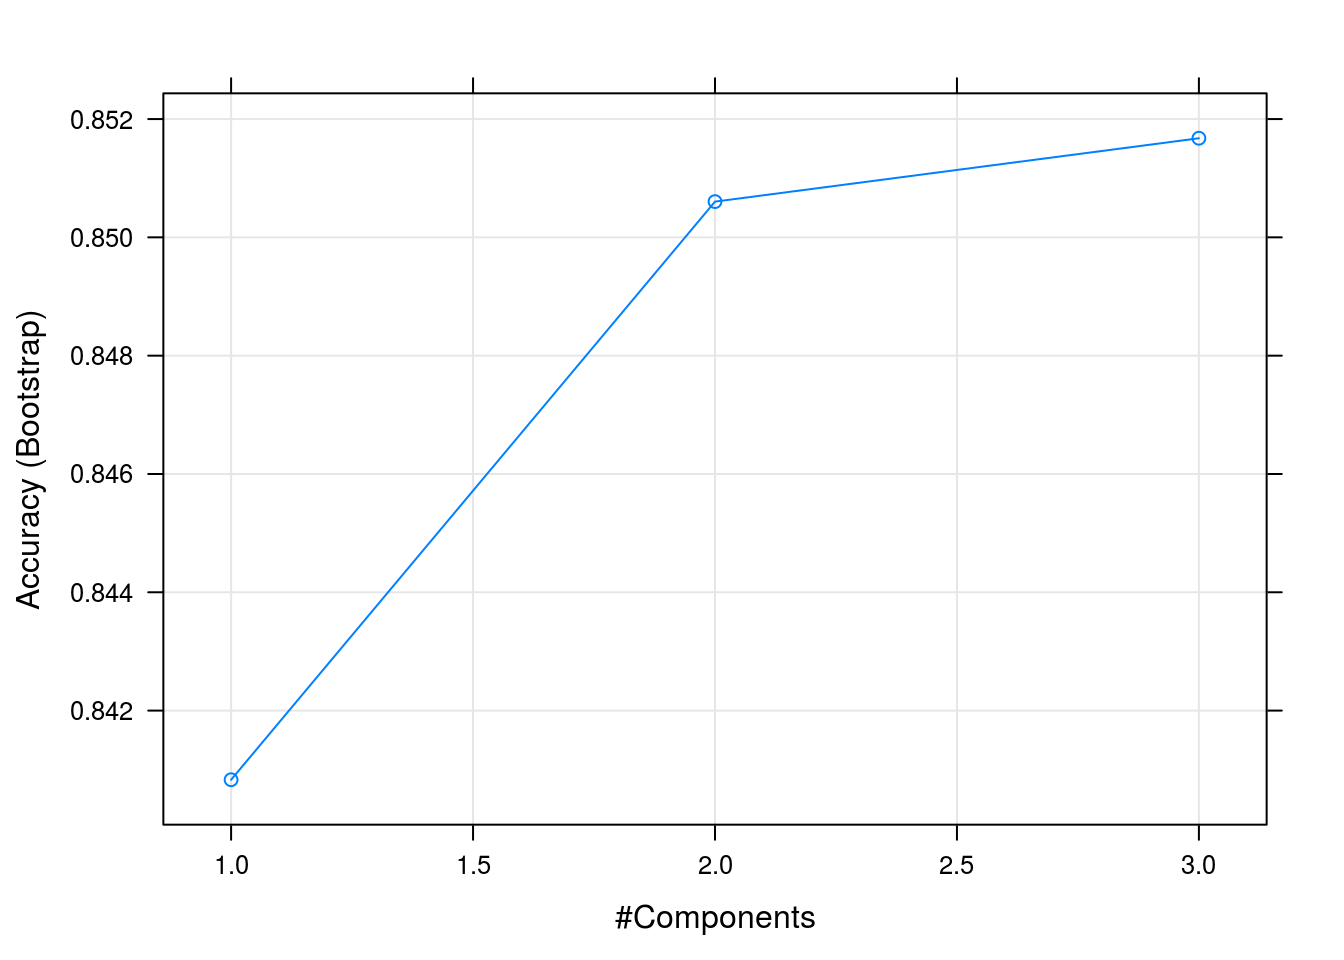
\includegraphics{DASE_files/figure-latex/unnamed-chunk-63-1.pdf}

The parameter \texttt{tuneLength} allow us to specify the number values
per parameter to consider.

\begin{Shaded}
\begin{Highlighting}[]
\NormalTok{plsFit3x10cv <-}\StringTok{ }\KeywordTok{train} \NormalTok{(Defective ~}\StringTok{ }\NormalTok{., }\DataTypeTok{data=}\NormalTok{kc1.train, }\DataTypeTok{method=}\StringTok{"pls"}\NormalTok{, }\DataTypeTok{trControl=}\NormalTok{ctrl, }\DataTypeTok{metric=}\StringTok{"ROC"}\NormalTok{, }\DataTypeTok{tuneLength=}\DecValTok{5}\NormalTok{, }\DataTypeTok{preProc=}\KeywordTok{c}\NormalTok{(}\StringTok{"center"}\NormalTok{,}\StringTok{"scale"}\NormalTok{))}

\NormalTok{plsFit3x10cv}
\end{Highlighting}
\end{Shaded}

\begin{verbatim}
## Partial Least Squares 
## 
## 1573 samples
##   21 predictors
##    2 classes: 'N', 'Y' 
## 
## Pre-processing: centered (21), scaled (21) 
## Resampling: Cross-Validated (10 fold, repeated 3 times) 
## Summary of sample sizes: 1415, 1416, 1417, 1415, 1416, 1416, ... 
## Resampling results across tuning parameters:
## 
##   ncomp  ROC    Sens   Spec  
##   1      0.788  0.981  0.0929
##   2      0.793  0.984  0.1311
##   3      0.790  0.982  0.1517
##   4      0.790  0.986  0.1626
##   5      0.789  0.985  0.1596
## 
## ROC was used to select the optimal model using  the largest value.
## The final value used for the model was ncomp = 2.
\end{verbatim}

\begin{Shaded}
\begin{Highlighting}[]
\KeywordTok{plot}\NormalTok{(plsFit3x10cv)}
\end{Highlighting}
\end{Shaded}

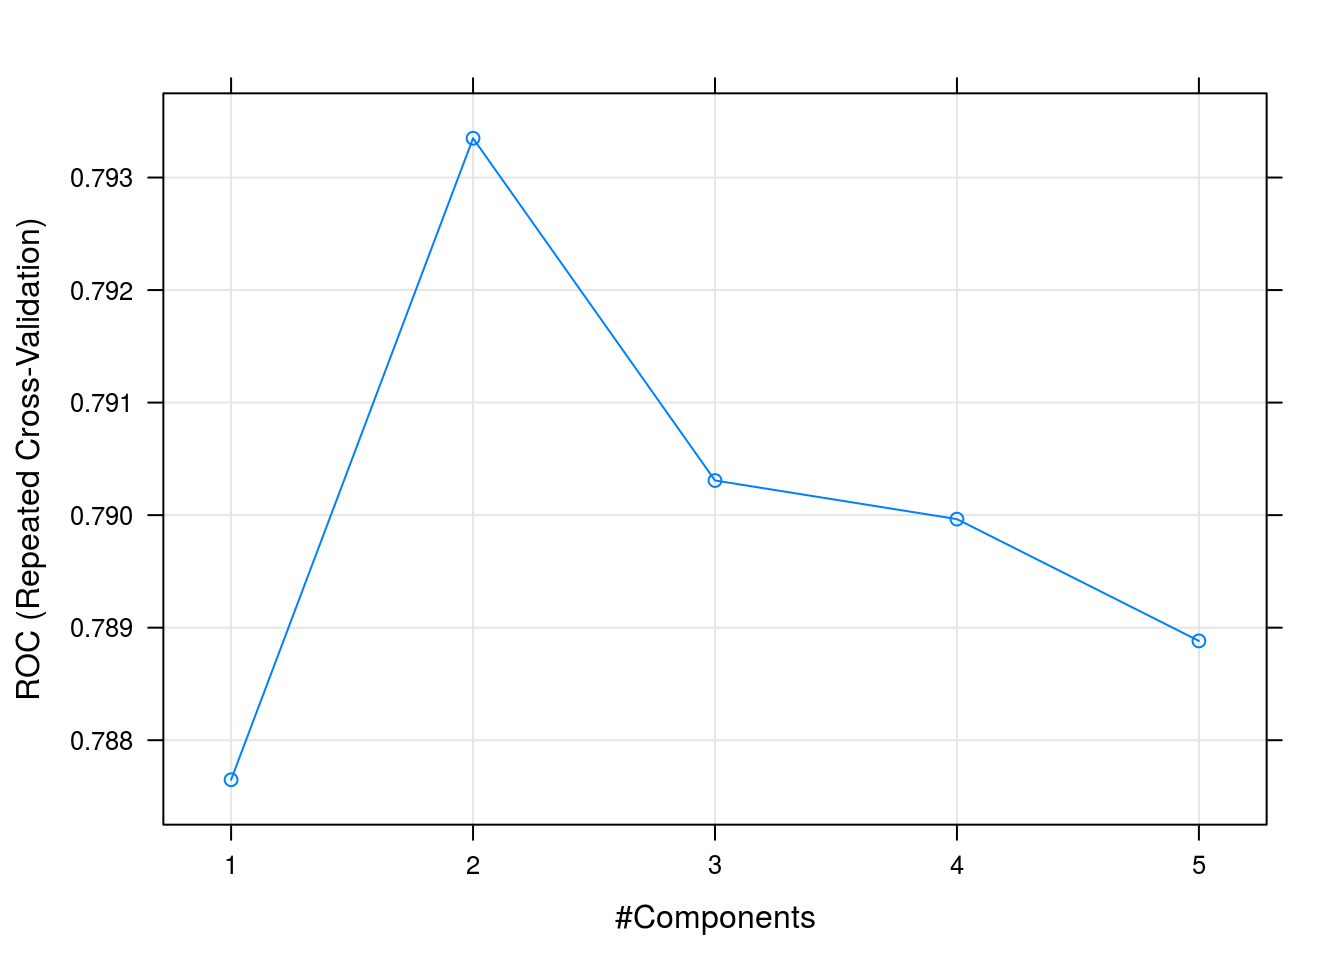
\includegraphics{DASE_files/figure-latex/unnamed-chunk-64-1.pdf}

Finally to predict new cases, \texttt{caret} will use the best classfier
obtained for prediction.

\begin{Shaded}
\begin{Highlighting}[]
\NormalTok{plsProbs <-}\StringTok{ }\KeywordTok{predict}\NormalTok{(plsFit3x10cv, }\DataTypeTok{newdata =} \NormalTok{kc1.test, }\DataTypeTok{type =} \StringTok{"prob"}\NormalTok{)}
\end{Highlighting}
\end{Shaded}

\begin{Shaded}
\begin{Highlighting}[]
\NormalTok{plsClasses <-}\StringTok{ }\KeywordTok{predict}\NormalTok{(plsFit3x10cv, }\DataTypeTok{newdata =} \NormalTok{kc1.test, }\DataTypeTok{type =} \StringTok{"raw"}\NormalTok{)}
\KeywordTok{confusionMatrix}\NormalTok{(}\DataTypeTok{data=}\NormalTok{plsClasses,kc1.test$Defective)}
\end{Highlighting}
\end{Shaded}

\begin{verbatim}
## Confusion Matrix and Statistics
## 
##           Reference
## Prediction   N   Y
##          N 439  69
##          Y   3  12
##                                        
##                Accuracy : 0.862        
##                  95% CI : (0.83, 0.891)
##     No Information Rate : 0.845        
##     P-Value [Acc > NIR] : 0.152        
##                                        
##                   Kappa : 0.212        
##  Mcnemar's Test P-Value : 1.85e-14     
##                                        
##             Sensitivity : 0.993        
##             Specificity : 0.148        
##          Pos Pred Value : 0.864        
##          Neg Pred Value : 0.800        
##              Prevalence : 0.845        
##          Detection Rate : 0.839        
##    Detection Prevalence : 0.971        
##       Balanced Accuracy : 0.571        
##                                        
##        'Positive' Class : N            
## 
\end{verbatim}

\subsection{Predicting the number of defects (numerical
class)}\label{predicting-the-number-of-defects-numerical-class}

From the Bug Predictiono Repository
\url{http://bug.inf.usi.ch/download.php}

Some datasets contain CK and other 11 object oriented metrics for the
last version of the system plus categorized (with severity and priority)
post-release defects. Using such dataset:

\begin{Shaded}
\begin{Highlighting}[]
\NormalTok{jdt <-}\StringTok{ }\KeywordTok{read.csv}\NormalTok{(}\StringTok{"./datasets/defectPred/BPD/single-version-ck-oo-EclipseJDTCore.csv"}\NormalTok{, }\DataTypeTok{sep=}\StringTok{";"}\NormalTok{)}

\CommentTok{# We just use the number of bugs, so we removed others}
\NormalTok{jdt$classname <-}\StringTok{ }\OtherTok{NULL}
\NormalTok{jdt$nonTrivialBugs <-}\StringTok{ }\OtherTok{NULL}
\NormalTok{jdt$majorBugs <-}\StringTok{ }\OtherTok{NULL}
\NormalTok{jdt$minorBugs <-}\StringTok{ }\OtherTok{NULL}
\NormalTok{jdt$criticalBugs <-}\StringTok{ }\OtherTok{NULL}
\NormalTok{jdt$highPriorityBugs <-}\StringTok{ }\OtherTok{NULL}
\NormalTok{jdt$X <-}\StringTok{ }\OtherTok{NULL}

\CommentTok{# Caret}
\KeywordTok{library}\NormalTok{(caret)}

\CommentTok{# Split data into training and test datasets}
\KeywordTok{set.seed}\NormalTok{(}\DecValTok{1}\NormalTok{)}
\NormalTok{inTrain <-}\StringTok{ }\KeywordTok{createDataPartition}\NormalTok{(}\DataTypeTok{y=}\NormalTok{jdt$bugs,}\DataTypeTok{p=}\NormalTok{.}\DecValTok{8}\NormalTok{,}\DataTypeTok{list=}\OtherTok{FALSE}\NormalTok{)}
\NormalTok{jdt.train <-}\StringTok{ }\NormalTok{jdt[inTrain,]}
\NormalTok{jdt.test <-}\StringTok{ }\NormalTok{jdt[-inTrain,]}
\end{Highlighting}
\end{Shaded}

\begin{Shaded}
\begin{Highlighting}[]
\NormalTok{ctrl <-}\StringTok{ }\KeywordTok{trainControl}\NormalTok{(}\DataTypeTok{method =} \StringTok{"repeatedcv"}\NormalTok{,}\DataTypeTok{repeats=}\DecValTok{3}\NormalTok{)}
\NormalTok{glmModel <-}\StringTok{ }\KeywordTok{train} \NormalTok{(bugs ~}\StringTok{ }\NormalTok{., }\DataTypeTok{data=}\NormalTok{jdt.train, }\DataTypeTok{method=}\StringTok{"glm"}\NormalTok{, }\DataTypeTok{trControl=}\NormalTok{ctrl, }\DataTypeTok{preProc=}\KeywordTok{c}\NormalTok{(}\StringTok{"center"}\NormalTok{,}\StringTok{"scale"}\NormalTok{))}
\NormalTok{glmModel}
\end{Highlighting}
\end{Shaded}

\begin{verbatim}
## Generalized Linear Model 
## 
## 798 samples
##  17 predictors
## 
## Pre-processing: centered (17), scaled (17) 
## Resampling: Cross-Validated (10 fold, repeated 3 times) 
## Summary of sample sizes: 718, 718, 718, 718, 719, 718, ... 
## Resampling results:
## 
##   RMSE   Rsquared
##   0.841  0.386   
## 
## 
\end{verbatim}

Others such as Elasticnet:

\begin{Shaded}
\begin{Highlighting}[]
\NormalTok{glmnetModel <-}\StringTok{ }\KeywordTok{train} \NormalTok{(bugs ~}\StringTok{ }\NormalTok{., }\DataTypeTok{data=}\NormalTok{jdt.train, }\DataTypeTok{method=}\StringTok{"glmnet"}\NormalTok{, }\DataTypeTok{trControl=}\NormalTok{ctrl, }\DataTypeTok{preProc=}\KeywordTok{c}\NormalTok{(}\StringTok{"center"}\NormalTok{,}\StringTok{"scale"}\NormalTok{))}
\end{Highlighting}
\end{Shaded}

\begin{verbatim}
## Loading required package: glmnet
\end{verbatim}

\begin{verbatim}
## Loading required package: Matrix
\end{verbatim}

\begin{verbatim}
## Loading required package: foreach
\end{verbatim}

\begin{verbatim}
## Loaded glmnet 2.0-5
\end{verbatim}

\begin{Shaded}
\begin{Highlighting}[]
\NormalTok{glmnetModel}
\end{Highlighting}
\end{Shaded}

\begin{verbatim}
## glmnet 
## 
## 798 samples
##  17 predictors
## 
## Pre-processing: centered (17), scaled (17) 
## Resampling: Cross-Validated (10 fold, repeated 3 times) 
## Summary of sample sizes: 718, 718, 718, 718, 718, 718, ... 
## Resampling results across tuning parameters:
## 
##   alpha  lambda  RMSE   Rsquared
##   0.10   0.0012  0.813  0.341   
##   0.10   0.0120  0.818  0.334   
##   0.10   0.1202  0.808  0.340   
##   0.55   0.0012  0.812  0.341   
##   0.55   0.0120  0.823  0.327   
##   0.55   0.1202  0.812  0.347   
##   1.00   0.0012  0.812  0.341   
##   1.00   0.0120  0.819  0.331   
##   1.00   0.1202  0.817  0.345   
## 
## RMSE was used to select the optimal model using  the smallest value.
## The final values used for the model were alpha = 0.1 and lambda = 0.12.
\end{verbatim}

\section{Binary Logistic Regression
(BLR)}\label{binary-logistic-regression-blr}

Binary Logistic Regression (BLR) can models fault-proneness as follows

\[fp(X) = \frac{e^{logit()}}{1 + e^{logit(X)}}\]

where the simplest form for logit is:

\(logit(X) = c_{0} + c_{1}X\)

\begin{Shaded}
\begin{Highlighting}[]
\NormalTok{jdt <-}\StringTok{ }\KeywordTok{read.csv}\NormalTok{(}\StringTok{"./datasets/defectPred/BPD/single-version-ck-oo-EclipseJDTCore.csv"}\NormalTok{, }\DataTypeTok{sep=}\StringTok{";"}\NormalTok{)}

\CommentTok{# Caret}
\KeywordTok{library}\NormalTok{(caret)}

\CommentTok{# Convert the response variable into a boolean variable (0/1)}
\NormalTok{jdt$bugs[jdt$bugs>=}\DecValTok{1}\NormalTok{]<-}\DecValTok{1}

\NormalTok{cbo <-}\StringTok{ }\NormalTok{jdt$cbo}
\NormalTok{bugs <-}\StringTok{ }\NormalTok{jdt$bugs}

\CommentTok{# Split data into training and test datasets}
\NormalTok{jdt2 =}\StringTok{ }\KeywordTok{data.frame}\NormalTok{(cbo, bugs)}
\NormalTok{inTrain <-}\StringTok{ }\KeywordTok{createDataPartition}\NormalTok{(}\DataTypeTok{y=}\NormalTok{jdt2$bugs,}\DataTypeTok{p=}\NormalTok{.}\DecValTok{8}\NormalTok{,}\DataTypeTok{list=}\OtherTok{FALSE}\NormalTok{)}
\NormalTok{jdtTrain <-}\StringTok{ }\NormalTok{jdt2[inTrain,]}
\NormalTok{jdtTest <-}\StringTok{ }\NormalTok{jdt2[-inTrain,]}
\end{Highlighting}
\end{Shaded}

BLR models fault-proneness are as follows

\[fp(X) = \frac{e^{logit()}}{1 + e^{logit(X)}}\]

where the simplest form for logit is:

\(logit(X) = c_{0} + c_{1}X\)

\begin{Shaded}
\begin{Highlighting}[]
\CommentTok{# logit regression}
\CommentTok{# glmLogit <- train (bugs ~ ., data=jdt.train, method="glm", family=binomial(link = logit))       }

\NormalTok{glmLogit <-}\StringTok{ }\KeywordTok{glm} \NormalTok{(bugs ~}\StringTok{ }\NormalTok{., }\DataTypeTok{data=}\NormalTok{jdtTrain, }\DataTypeTok{family=}\KeywordTok{binomial}\NormalTok{(}\DataTypeTok{link =} \NormalTok{logit))}
\KeywordTok{summary}\NormalTok{(glmLogit)}
\end{Highlighting}
\end{Shaded}

\begin{verbatim}
## 
## Call:
## glm(formula = bugs ~ ., family = binomial(link = logit), data = jdtTrain)
## 
## Deviance Residuals: 
##    Min      1Q  Median      3Q     Max  
## -3.573  -0.613  -0.538  -0.497   2.099  
## 
## Coefficients:
##             Estimate Std. Error z value Pr(>|z|)    
## (Intercept) -2.08638    0.13462  -15.50  < 2e-16 ***
## cbo          0.05646    0.00705    8.01  1.1e-15 ***
## ---
## Signif. codes:  0 '***' 0.001 '**' 0.01 '*' 0.05 '.' 0.1 ' ' 1
## 
## (Dispersion parameter for binomial family taken to be 1)
## 
##     Null deviance: 831.84  on 797  degrees of freedom
## Residual deviance: 725.93  on 796  degrees of freedom
## AIC: 729.9
## 
## Number of Fisher Scoring iterations: 5
\end{verbatim}

Predict a single point:

\begin{Shaded}
\begin{Highlighting}[]
\NormalTok{newData =}\StringTok{ }\KeywordTok{data.frame}\NormalTok{(}\DataTypeTok{cbo =} \DecValTok{3}\NormalTok{)}
\KeywordTok{predict}\NormalTok{(glmLogit, newData, }\DataTypeTok{type =} \StringTok{"response"}\NormalTok{)}
\end{Highlighting}
\end{Shaded}

\begin{verbatim}
##     1 
## 0.128
\end{verbatim}

Draw the results, modified from:
\url{http://www.shizukalab.com/toolkits/plotting-logistic-regression-in-r}

\begin{Shaded}
\begin{Highlighting}[]
\NormalTok{results <-}\StringTok{ }\KeywordTok{predict}\NormalTok{(glmLogit, jdtTest, }\DataTypeTok{type =} \StringTok{"response"}\NormalTok{)}

\KeywordTok{range}\NormalTok{(jdtTrain$cbo)}
\end{Highlighting}
\end{Shaded}

\begin{verbatim}
## [1]   0 156
\end{verbatim}

\begin{Shaded}
\begin{Highlighting}[]
\KeywordTok{range}\NormalTok{(results)}
\end{Highlighting}
\end{Shaded}

\begin{verbatim}
## [1] 0.110 0.984
\end{verbatim}

\begin{Shaded}
\begin{Highlighting}[]
\KeywordTok{plot}\NormalTok{(jdt2$cbo,jdt2$bugs)}
\KeywordTok{curve}\NormalTok{(}\KeywordTok{predict}\NormalTok{(glmLogit, }\KeywordTok{data.frame}\NormalTok{(}\DataTypeTok{cbo=}\NormalTok{x), }\DataTypeTok{type =} \StringTok{"response"}\NormalTok{),}\DataTypeTok{add=}\OtherTok{TRUE}\NormalTok{)}
\end{Highlighting}
\end{Shaded}

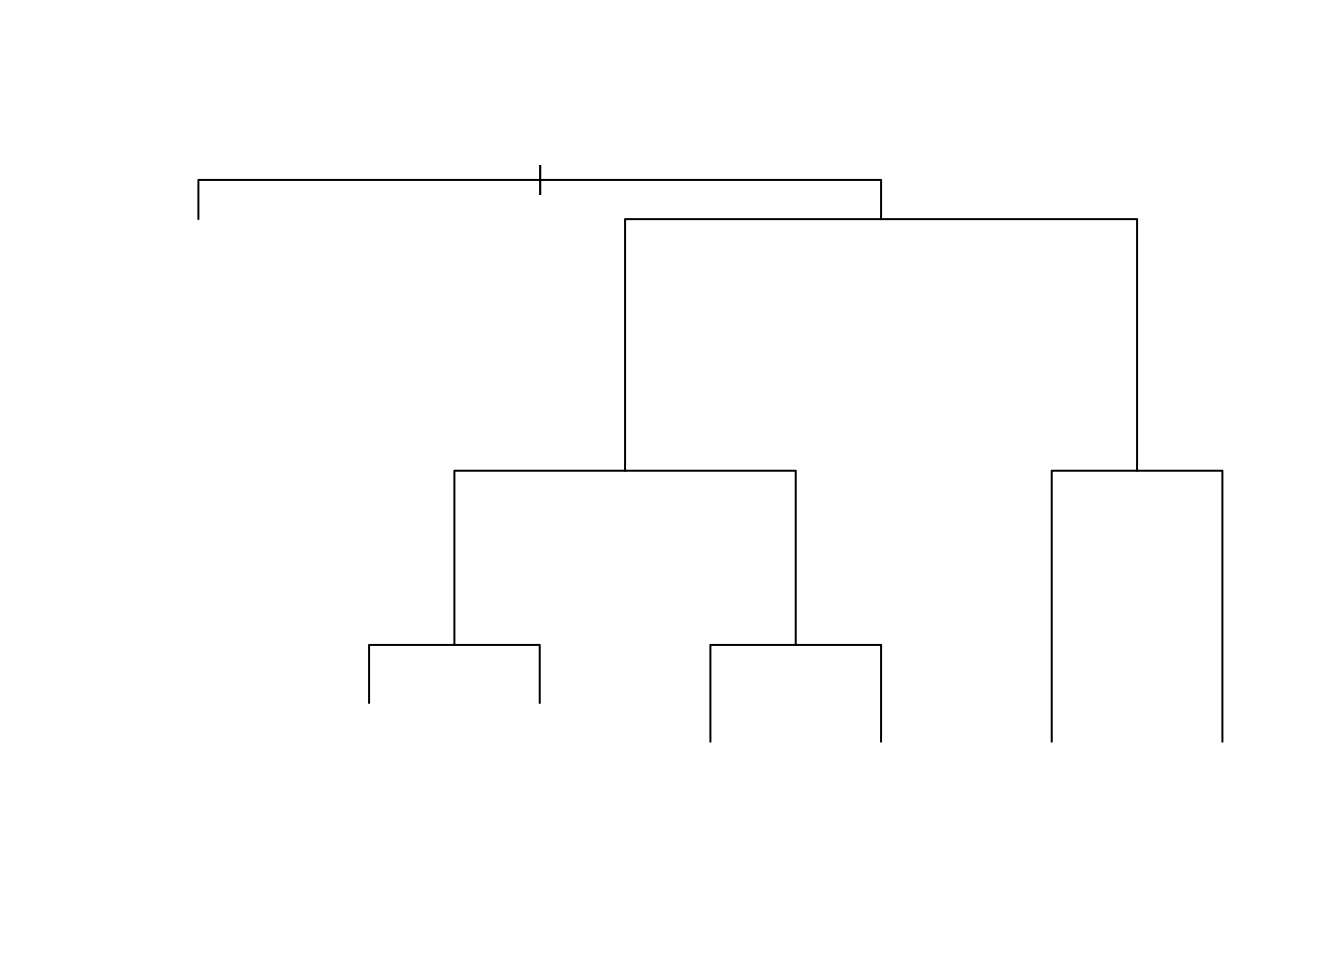
\includegraphics{DASE_files/figure-latex/unnamed-chunk-73-1.pdf}

\begin{Shaded}
\begin{Highlighting}[]
\CommentTok{# points(jdtTrain$cbo,fitted(glmLogit))}
\end{Highlighting}
\end{Shaded}

Another type of graph:

\begin{Shaded}
\begin{Highlighting}[]
\KeywordTok{library}\NormalTok{(popbio)}
\end{Highlighting}
\end{Shaded}

\begin{verbatim}
## 
## Attaching package: 'popbio'
\end{verbatim}

\begin{verbatim}
## The following object is masked from 'package:caret':
## 
##     sensitivity
\end{verbatim}

\begin{Shaded}
\begin{Highlighting}[]
\KeywordTok{logi.hist.plot}\NormalTok{(jdt2$cbo,jdt2$bugs,}\DataTypeTok{boxp=}\OtherTok{FALSE}\NormalTok{,}\DataTypeTok{type=}\StringTok{"hist"}\NormalTok{,}\DataTypeTok{col=}\StringTok{"gray"}\NormalTok{)}
\end{Highlighting}
\end{Shaded}

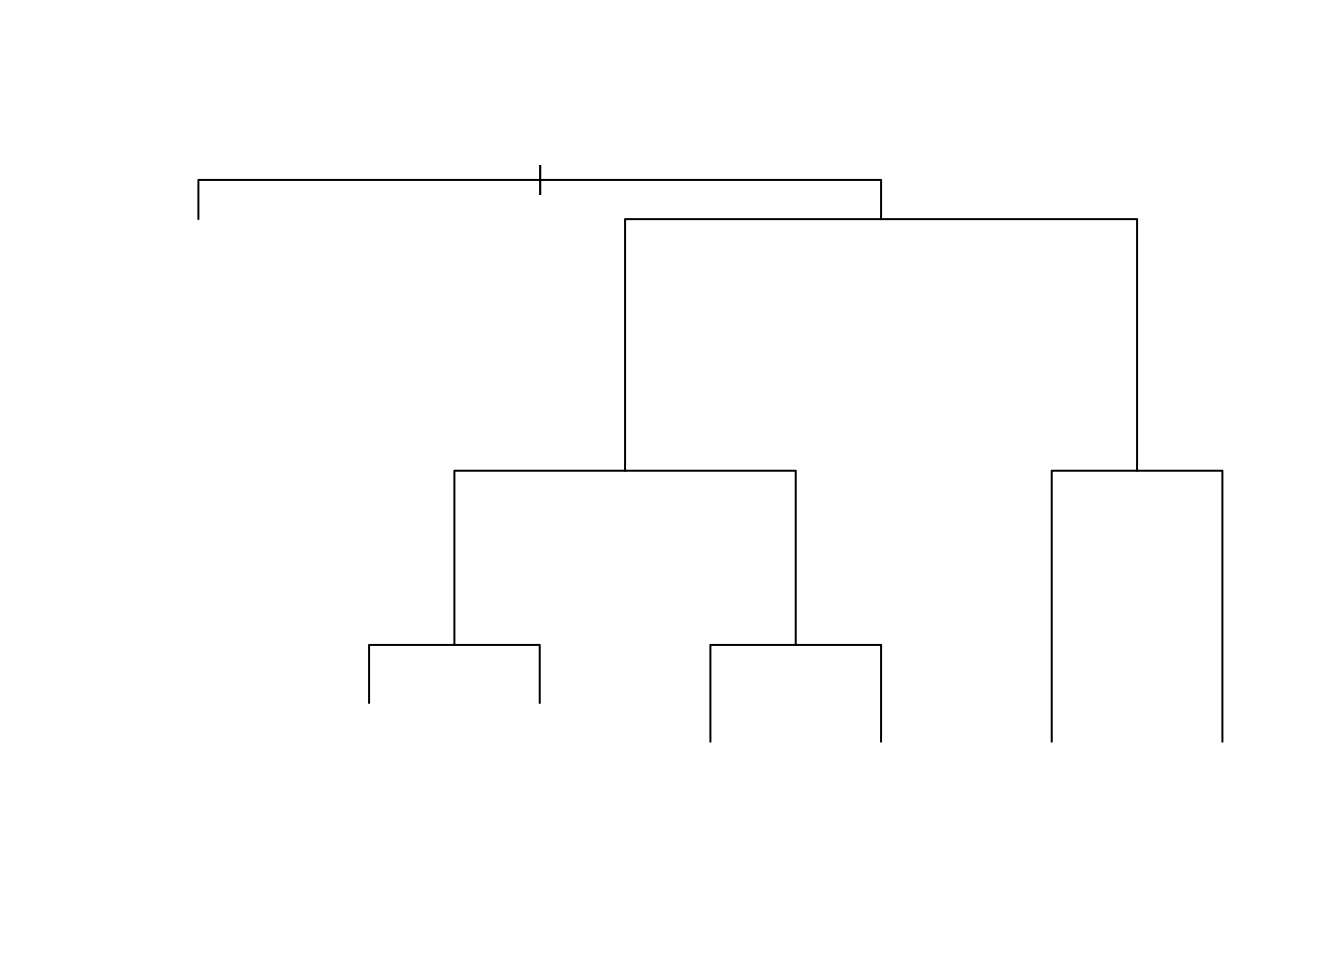
\includegraphics{DASE_files/figure-latex/unnamed-chunk-74-1.pdf}

\section{Classification Trees}\label{classification-trees}

There are several packages for inducing classification trees, for
example with the
\href{https://cran.r-project.org/web/packages/party/index.html}{party
package} (recursive partitioning):

\begin{Shaded}
\begin{Highlighting}[]
\CommentTok{# Build a decision tree}
\KeywordTok{library}\NormalTok{(party)}

\NormalTok{kc2 <-}\StringTok{ }\KeywordTok{read.arff}\NormalTok{(}\StringTok{"./datasets/defectPred/D1/MC1.arff"}\NormalTok{)}
\KeywordTok{str}\NormalTok{(kc2)}
\end{Highlighting}
\end{Shaded}

\begin{verbatim}
## 'data.frame':    9277 obs. of  39 variables:
##  $ LOC_BLANK                      : num  0 0 0 0 0 0 0 0 0 0 ...
##  $ BRANCH_COUNT                   : num  1 1 1 1 1 1 1 1 1 1 ...
##  $ CALL_PAIRS                     : num  0 0 0 0 0 0 0 0 0 0 ...
##  $ LOC_CODE_AND_COMMENT           : num  0 0 0 0 0 0 0 0 0 0 ...
##  $ LOC_COMMENTS                   : num  0 0 0 0 0 0 0 0 0 0 ...
##  $ CONDITION_COUNT                : num  0 0 0 0 0 0 0 0 0 0 ...
##  $ CYCLOMATIC_COMPLEXITY          : num  1 1 1 1 1 1 1 1 1 1 ...
##  $ CYCLOMATIC_DENSITY             : num  1 1 1 1 1 1 1 1 1 1 ...
##  $ DECISION_COUNT                 : num  0 0 0 0 0 0 0 0 0 0 ...
##  $ DESIGN_COMPLEXITY              : num  1 1 1 1 1 1 1 1 1 1 ...
##  $ DESIGN_DENSITY                 : num  1 1 1 1 1 1 1 1 1 1 ...
##  $ EDGE_COUNT                     : num  1 1 1 1 1 1 1 1 1 1 ...
##  $ ESSENTIAL_COMPLEXITY           : num  1 1 1 1 1 1 1 1 1 1 ...
##  $ ESSENTIAL_DENSITY              : num  0 0 0 0 0 0 0 0 0 0 ...
##  $ LOC_EXECUTABLE                 : num  0 0 0 0 0 0 0 0 0 0 ...
##  $ PARAMETER_COUNT                : num  0 0 0 0 0 0 0 0 0 0 ...
##  $ GLOBAL_DATA_COMPLEXITY         : num  0 0 0 0 0 0 0 0 0 0 ...
##  $ GLOBAL_DATA_DENSITY            : num  0 0 0 0 0 0 0 0 0 0 ...
##  $ HALSTEAD_CONTENT               : num  0 0 0 0 0 0 0 0 0 0 ...
##  $ HALSTEAD_DIFFICULTY            : num  0 0 0 0 0 0 0 0 0 0 ...
##  $ HALSTEAD_EFFORT                : num  0 0 0 0 0 0 0 0 0 0 ...
##  $ HALSTEAD_ERROR_EST             : num  0 0 0 0 0 0 0 0 0 0 ...
##  $ HALSTEAD_LENGTH                : num  1 1 0 0 1 1 0 0 1 1 ...
##  $ HALSTEAD_LEVEL                 : num  0 0 0 0 0 0 0 0 0 0 ...
##  $ HALSTEAD_PROG_TIME             : num  0 0 0 0 0 0 0 0 0 0 ...
##  $ HALSTEAD_VOLUME                : num  0 0 0 0 0 0 0 0 0 0 ...
##  $ MAINTENANCE_SEVERITY           : num  1 1 1 1 1 1 1 1 1 1 ...
##  $ MODIFIED_CONDITION_COUNT       : num  0 0 0 0 0 0 0 0 0 0 ...
##  $ MULTIPLE_CONDITION_COUNT       : num  0 0 0 0 0 0 0 0 0 0 ...
##  $ NODE_COUNT                     : num  2 2 2 2 2 2 2 2 2 2 ...
##  $ NORMALIZED_CYLOMATIC_COMPLEXITY: num  1 1 1 1 1 1 1 1 1 1 ...
##  $ NUM_OPERANDS                   : num  0 0 0 0 0 0 0 0 0 0 ...
##  $ NUM_OPERATORS                  : num  1 1 0 0 1 1 0 0 1 1 ...
##  $ NUM_UNIQUE_OPERANDS            : num  0 0 0 0 0 0 0 0 0 0 ...
##  $ NUM_UNIQUE_OPERATORS           : num  1 1 0 0 1 1 0 0 1 1 ...
##  $ NUMBER_OF_LINES                : num  1 1 1 1 1 1 1 1 1 1 ...
##  $ PERCENT_COMMENTS               : num  0 0 0 0 0 0 0 0 0 0 ...
##  $ LOC_TOTAL                      : num  0 0 0 0 0 0 0 0 0 0 ...
##  $ Defective                      : Factor w/ 2 levels "N","Y": 1 1 1 1 1 1 1 1 1 1 ...
\end{verbatim}

\begin{Shaded}
\begin{Highlighting}[]
\KeywordTok{set.seed}\NormalTok{(}\DecValTok{1}\NormalTok{)}
\NormalTok{inTrain <-}\StringTok{ }\KeywordTok{createDataPartition}\NormalTok{(}\DataTypeTok{y=}\NormalTok{kc2$Defective,}\DataTypeTok{p=}\NormalTok{.}\DecValTok{60}\NormalTok{,}\DataTypeTok{list=}\OtherTok{FALSE}\NormalTok{)}
\NormalTok{kc2.train <-}\StringTok{ }\NormalTok{kc2[inTrain,]}
\NormalTok{kc2.test <-}\StringTok{ }\NormalTok{kc2[-inTrain,]}

\NormalTok{kc2.formula <-}\StringTok{ }\NormalTok{kc2$Defective ~}\StringTok{ }\NormalTok{.}
\NormalTok{kc2.ctree <-}\StringTok{ }\KeywordTok{ctree}\NormalTok{(kc2.formula, }\DataTypeTok{data =} \NormalTok{kc2.train)}

\CommentTok{# predict on test data}
\NormalTok{pred <-}\StringTok{ }\KeywordTok{predict}\NormalTok{(kc2.ctree, }\DataTypeTok{newdata =} \NormalTok{kc2.test)}
\CommentTok{# check prediction result}
\KeywordTok{table}\NormalTok{(pred, kc2.test$Defective)}
\end{Highlighting}
\end{Shaded}

\begin{verbatim}
##     
## pred    N    Y
##    N 3683   27
##    Y    0    0
\end{verbatim}

\begin{Shaded}
\begin{Highlighting}[]
\KeywordTok{plot}\NormalTok{(kc2.ctree)}
\end{Highlighting}
\end{Shaded}

\includegraphics{DASE_files/figure-latex/unnamed-chunk-75-1.pdf}

Using the C50, there are two ways, specifying train and testing

\begin{Shaded}
\begin{Highlighting}[]
\KeywordTok{library}\NormalTok{(C50)}
\NormalTok{c50t <-}\StringTok{ }\KeywordTok{C5.0}\NormalTok{(kc1.train[,-}\KeywordTok{ncol}\NormalTok{(kc1.train)], kc1.train[,}\KeywordTok{ncol}\NormalTok{(kc1.train)])}
\KeywordTok{summary}\NormalTok{(c50t)}
\end{Highlighting}
\end{Shaded}

\begin{verbatim}
## 
## Call:
## C5.0.default(x = kc1.train[, -ncol(kc1.train)], y =
##  kc1.train[, ncol(kc1.train)])
## 
## 
## C5.0 [Release 2.07 GPL Edition]      Tue Apr  4 20:02:04 2017
## -------------------------------
## 
## Class specified by attribute `outcome'
## 
## Read 1573 cases (22 attributes) from undefined.data
## 
## Decision tree:
## 
## LOC_EXECUTABLE <= 4: N (745/22)
## LOC_EXECUTABLE > 4:
## :...HALSTEAD_ERROR_EST <= 0.36: N (734/169)
##     HALSTEAD_ERROR_EST > 0.36:
##     :...DESIGN_COMPLEXITY > 19: N (6)
##         DESIGN_COMPLEXITY <= 19:
##         :...LOC_CODE_AND_COMMENT <= 1: Y (71/22)
##             LOC_CODE_AND_COMMENT > 1: N (17/4)
## 
## 
## Evaluation on training data (1573 cases):
## 
##      Decision Tree   
##    ----------------  
##    Size      Errors  
## 
##       5  217(13.8%)   <<
## 
## 
##     (a)   (b)    <-classified as
##    ----  ----
##    1307    22    (a): class N
##     195    49    (b): class Y
## 
## 
##  Attribute usage:
## 
##  100.00% LOC_EXECUTABLE
##   52.64% HALSTEAD_ERROR_EST
##    5.98% DESIGN_COMPLEXITY
##    5.59% LOC_CODE_AND_COMMENT
## 
## 
## Time: 0.0 secs
\end{verbatim}

\begin{Shaded}
\begin{Highlighting}[]
\KeywordTok{plot}\NormalTok{(c50t)}
\end{Highlighting}
\end{Shaded}

\includegraphics{DASE_files/figure-latex/unnamed-chunk-76-1.pdf}

\begin{Shaded}
\begin{Highlighting}[]
\NormalTok{c50tPred <-}\StringTok{ }\KeywordTok{predict}\NormalTok{(c50t, kc1.train)}
\KeywordTok{table}\NormalTok{(c50tPred, kc1.train$Defective)}
\end{Highlighting}
\end{Shaded}

\begin{verbatim}
##         
## c50tPred    N    Y
##        N 1307  195
##        Y   22   49
\end{verbatim}

or using the formula approach:

\begin{Shaded}
\begin{Highlighting}[]
\CommentTok{# Using the formula notation}
\NormalTok{c50t2 <-}\StringTok{ }\KeywordTok{C5.0}\NormalTok{(Defective ~}\StringTok{ }\NormalTok{., kc1.train)}
\NormalTok{c50tPred2 <-}\StringTok{ }\KeywordTok{predict}\NormalTok{(c50t2, kc1.train)}
\KeywordTok{table}\NormalTok{(c50tPred2, kc1.train$Defective)}
\end{Highlighting}
\end{Shaded}

\begin{verbatim}
##          
## c50tPred2    N    Y
##         N 1307  195
##         Y   22   49
\end{verbatim}

Using the
\href{https://cran.r-project.org/web/packages/rpart/index.html}{`rpart'
package}

\begin{Shaded}
\begin{Highlighting}[]
\CommentTok{# Using the 'rpart' package}
\KeywordTok{library}\NormalTok{(rpart)}
\NormalTok{kc1.rpart <-}\StringTok{ }\KeywordTok{rpart}\NormalTok{(Defective ~}\StringTok{ }\NormalTok{., }\DataTypeTok{data=}\NormalTok{kc1.train)}
\KeywordTok{plot}\NormalTok{(kc1.rpart)}
\end{Highlighting}
\end{Shaded}

\includegraphics{DASE_files/figure-latex/unnamed-chunk-78-1.pdf}

\begin{Shaded}
\begin{Highlighting}[]
\KeywordTok{library}\NormalTok{(rpart.plot)}
\CommentTok{#asRules(kc1.rpart)}
\CommentTok{#fancyRpartPlot(kc1.rpart)}
\end{Highlighting}
\end{Shaded}

\section{Rules}\label{rules}

C5 Rules

\begin{Shaded}
\begin{Highlighting}[]
\KeywordTok{library}\NormalTok{(C50)}
\NormalTok{c50r <-}\StringTok{ }\KeywordTok{C5.0}\NormalTok{(kc1.train[,-}\KeywordTok{ncol}\NormalTok{(kc1.train)], kc1.train[,}\KeywordTok{ncol}\NormalTok{(kc1.train)], }\DataTypeTok{rules =} \OtherTok{TRUE}\NormalTok{)}
\KeywordTok{summary}\NormalTok{(c50r)}
\end{Highlighting}
\end{Shaded}

\begin{verbatim}
## 
## Call:
## C5.0.default(x = kc1.train[, -ncol(kc1.train)], y =
##  kc1.train[, ncol(kc1.train)], rules = TRUE)
## 
## 
## C5.0 [Release 2.07 GPL Edition]      Tue Apr  4 20:02:06 2017
## -------------------------------
## 
## Class specified by attribute `outcome'
## 
## Read 1573 cases (22 attributes) from undefined.data
## 
## Rules:
## 
## Rule 1: (1479/191, lift 1.0)
##  HALSTEAD_ERROR_EST <= 0.36
##  ->  class N  [0.870]
## 
## Rule 2: (94/41, lift 3.6)
##  HALSTEAD_ERROR_EST > 0.36
##  ->  class Y  [0.563]
## 
## Default class: N
## 
## 
## Evaluation on training data (1573 cases):
## 
##          Rules     
##    ----------------
##      No      Errors
## 
##       2  232(14.7%)   <<
## 
## 
##     (a)   (b)    <-classified as
##    ----  ----
##    1288    41    (a): class N
##     191    53    (b): class Y
## 
## 
##  Attribute usage:
## 
##  100.00% HALSTEAD_ERROR_EST
## 
## 
## Time: 0.0 secs
\end{verbatim}

\begin{Shaded}
\begin{Highlighting}[]
\NormalTok{c50rPred <-}\StringTok{ }\KeywordTok{predict}\NormalTok{(c50r, kc1.train)}
\KeywordTok{table}\NormalTok{(c50rPred, kc1.train$Defective)}
\end{Highlighting}
\end{Shaded}

\begin{verbatim}
##         
## c50rPred    N    Y
##        N 1288  191
##        Y   41   53
\end{verbatim}

\section{Distanced-based Methods}\label{distanced-based-methods}

In this case, there is no model as such. Given a new instance to
classify, this approach finds the closest \(k\)-neighbours to the given
instance.

\begin{Shaded}
\begin{Highlighting}[]
\KeywordTok{library}\NormalTok{(class)}

\NormalTok{ind <-}\StringTok{ }\KeywordTok{sample}\NormalTok{(}\DecValTok{2}\NormalTok{, }\KeywordTok{nrow}\NormalTok{(iris), }\DataTypeTok{replace=}\NormalTok{T, }\DataTypeTok{prob=}\KeywordTok{c}\NormalTok{(}\FloatTok{0.7}\NormalTok{, }\FloatTok{0.3}\NormalTok{))}
\NormalTok{kc1.train <-}\StringTok{ }\NormalTok{kc1[ind==}\DecValTok{1}\NormalTok{, ]}
\NormalTok{kc1.test <-}\StringTok{ }\NormalTok{kc1[ind==}\DecValTok{2}\NormalTok{, ]}

\NormalTok{m1 <-}\StringTok{ }\KeywordTok{knn}\NormalTok{(}\DataTypeTok{train=}\NormalTok{kc1.train[,-}\DecValTok{22}\NormalTok{], }\DataTypeTok{test=}\NormalTok{kc1.test[,-}\DecValTok{22}\NormalTok{], }\DataTypeTok{cl=}\NormalTok{kc1.train[,}\DecValTok{22}\NormalTok{], }\DataTypeTok{k=}\DecValTok{3}\NormalTok{)}

\KeywordTok{table}\NormalTok{(kc1.test[,}\DecValTok{22}\NormalTok{],m1)}
\end{Highlighting}
\end{Shaded}

\begin{verbatim}
##    m1
##       N   Y
##   N 455  24
##   Y  64  15
\end{verbatim}

\section{Probabilistic Methods}\label{probabilistic-methods}

\subsection{Naive Bayes}\label{naive-bayes}

Using the \texttt{klaR} package with \texttt{caret}:

\begin{Shaded}
\begin{Highlighting}[]
\KeywordTok{library}\NormalTok{(caret)}
\KeywordTok{library}\NormalTok{(klaR)}
\NormalTok{model <-}\StringTok{ }\KeywordTok{NaiveBayes}\NormalTok{(Defective ~}\StringTok{ }\NormalTok{., }\DataTypeTok{data =} \NormalTok{kc1.train)}
\NormalTok{predictions <-}\StringTok{ }\KeywordTok{predict}\NormalTok{(model, kc1.test[,-}\DecValTok{22}\NormalTok{])}
\KeywordTok{confusionMatrix}\NormalTok{(predictions$class, kc1.test$Defective)}
\end{Highlighting}
\end{Shaded}

\begin{verbatim}
## Confusion Matrix and Statistics
## 
##           Reference
## Prediction   N   Y
##          N 442  53
##          Y  37  26
##                                         
##                Accuracy : 0.839         
##                  95% CI : (0.806, 0.868)
##     No Information Rate : 0.858         
##     P-Value [Acc > NIR] : 0.917         
##                                         
##                   Kappa : 0.275         
##  Mcnemar's Test P-Value : 0.114         
##                                         
##             Sensitivity : 0.923         
##             Specificity : 0.329         
##          Pos Pred Value : 0.893         
##          Neg Pred Value : 0.413         
##              Prevalence : 0.858         
##          Detection Rate : 0.792         
##    Detection Prevalence : 0.887         
##       Balanced Accuracy : 0.626         
##                                         
##        'Positive' Class : N             
## 
\end{verbatim}

Using the \texttt{e1071} package:

\begin{Shaded}
\begin{Highlighting}[]
\KeywordTok{library} \NormalTok{(e1071)}
\NormalTok{n1 <-}\KeywordTok{naiveBayes}\NormalTok{(kc1.train$Defective ~}\StringTok{ }\NormalTok{., }\DataTypeTok{data=}\NormalTok{kc1.train)}

\CommentTok{# Show first 3 results using 'class'}
\KeywordTok{head}\NormalTok{(}\KeywordTok{predict}\NormalTok{(n1,kc1.test, }\DataTypeTok{type =} \KeywordTok{c}\NormalTok{(}\StringTok{"class"}\NormalTok{)),}\DecValTok{3}\NormalTok{) }\CommentTok{# class by default}
\end{Highlighting}
\end{Shaded}

\begin{verbatim}
## [1] N N N
## Levels: N Y
\end{verbatim}

\begin{Shaded}
\begin{Highlighting}[]
\CommentTok{# Show first 3 results using 'raw'}
\KeywordTok{head}\NormalTok{(}\KeywordTok{predict}\NormalTok{(n1,kc1.test, }\DataTypeTok{type =} \KeywordTok{c}\NormalTok{(}\StringTok{"raw"}\NormalTok{)),}\DecValTok{3}\NormalTok{)}
\end{Highlighting}
\end{Shaded}

\begin{verbatim}
##      N        Y
## [1,] 1 2.40e-09
## [2,] 1 5.76e-09
## [3,] 1 5.76e-09
\end{verbatim}

\subsection{Bayesian Networks}\label{bayesian-networks}

To Do

\part{Unsupervised Models}\label{part-unsupervised-models}

\chapter{Unsupervised or Descriptive
modeling}\label{unsupervised-or-descriptive-modeling}

From the descriptive (unsupervised) point of view, patterns are found to
predict future behaviour or estimate. This include association rules,
clustering, or tree clustering which aim at grouping together objects
(e.g., animals) into successively larger clusters, using some measure of
similarity or distance. The dataset will be as the previous table
without the \(C\) class attribute

\begin{longtable}[]{@{}lll@{}}
\toprule
Att\textsubscript{1} & & Att\textsubscript{n}\tabularnewline
\midrule
\endhead
a\textsubscript{11} & \ldots{} & a\textsubscript{1n}\tabularnewline
a\textsubscript{21} & \ldots{} & a\textsubscript{2n}\tabularnewline
\ldots{} & \ldots{} & \ldots{}\tabularnewline
a\textsubscript{m1} & \ldots{} & a\textsubscript{mn}\tabularnewline
\bottomrule
\end{longtable}

\section{Clustering}\label{clustering}

\begin{Shaded}
\begin{Highlighting}[]
\KeywordTok{library}\NormalTok{(foreign)}
\KeywordTok{library}\NormalTok{(fpc)}

\NormalTok{kc1 <-}\StringTok{ }\KeywordTok{read.arff}\NormalTok{(}\StringTok{"./datasets/defectPred/D1/KC1.arff"}\NormalTok{)}

\CommentTok{# Split into training and test datasets}
\KeywordTok{set.seed}\NormalTok{(}\DecValTok{1}\NormalTok{)}
\NormalTok{ind <-}\StringTok{ }\KeywordTok{sample}\NormalTok{(}\DecValTok{2}\NormalTok{, }\KeywordTok{nrow}\NormalTok{(kc1), }\DataTypeTok{replace =} \OtherTok{TRUE}\NormalTok{, }\DataTypeTok{prob =} \KeywordTok{c}\NormalTok{(}\FloatTok{0.7}\NormalTok{, }\FloatTok{0.3}\NormalTok{))}
\NormalTok{kc1.train <-}\StringTok{ }\NormalTok{kc1[ind==}\DecValTok{1}\NormalTok{, ]}
\NormalTok{kc1.test <-}\StringTok{ }\NormalTok{kc1[ind==}\DecValTok{2}\NormalTok{, ]}

\CommentTok{# No class}
\NormalTok{kc1.train$Defective <-}\StringTok{ }\OtherTok{NULL}

\NormalTok{ds <-}\StringTok{ }\KeywordTok{dbscan}\NormalTok{(kc1.train, }\DataTypeTok{eps =} \FloatTok{0.42}\NormalTok{, }\DataTypeTok{MinPts =} \DecValTok{5}\NormalTok{)}

\NormalTok{kc1.kmeans <-}\StringTok{ }\KeywordTok{kmeans}\NormalTok{(kc1.train, }\DecValTok{2}\NormalTok{)}
\end{Highlighting}
\end{Shaded}

\subsection{k-Means}\label{k-means}

\begin{Shaded}
\begin{Highlighting}[]
\KeywordTok{library}\NormalTok{(reshape, }\DataTypeTok{quietly=}\OtherTok{TRUE}\NormalTok{)}
\NormalTok{kc1.kmeans <-}\StringTok{ }\KeywordTok{kmeans}\NormalTok{(}\KeywordTok{sapply}\NormalTok{(}\KeywordTok{na.omit}\NormalTok{(kc1.train), rescaler, }\StringTok{"range"}\NormalTok{), }\DecValTok{10}\NormalTok{)}
\end{Highlighting}
\end{Shaded}

\section{Association rules}\label{association-rules}

\begin{Shaded}
\begin{Highlighting}[]
\KeywordTok{library}\NormalTok{(arules)}

\NormalTok{x <-}\StringTok{ }\KeywordTok{as.numeric}\NormalTok{(kc1$LOC_TOTAL)}
\KeywordTok{str}\NormalTok{(x)}
\end{Highlighting}
\end{Shaded}

\begin{verbatim}
##  num [1:2096] 5 3 3 3 12 5 3 3 3 13 ...
\end{verbatim}

\begin{Shaded}
\begin{Highlighting}[]
\KeywordTok{summary}\NormalTok{(x)}
\end{Highlighting}
\end{Shaded}

\begin{verbatim}
##    Min. 1st Qu.  Median    Mean 3rd Qu.    Max. 
##     1.0     3.0     9.0    20.4    24.0   288.0
\end{verbatim}

\begin{Shaded}
\begin{Highlighting}[]
\KeywordTok{hist}\NormalTok{(x, }\DataTypeTok{breaks=}\DecValTok{30}\NormalTok{, }\DataTypeTok{main=}\StringTok{"LoC Total"}\NormalTok{)}
\end{Highlighting}
\end{Shaded}

\includegraphics{DASE_files/figure-latex/unnamed-chunk-85-1.pdf}

\begin{Shaded}
\begin{Highlighting}[]
 \NormalTok{xDisc <-}\StringTok{ }\KeywordTok{discretize}\NormalTok{(x, }\DataTypeTok{categories=}\DecValTok{5}\NormalTok{)}
\CommentTok{# table(xDisc)}

 \NormalTok{for(i in }\DecValTok{1}\NormalTok{:}\DecValTok{21}\NormalTok{) kc1[,i] <-}\StringTok{ }\KeywordTok{discretize}\NormalTok{(kc1[,i],  }\StringTok{"frequency"}\NormalTok{, }\DataTypeTok{categories=}\DecValTok{5}\NormalTok{)}

\KeywordTok{str}\NormalTok{(kc1)}
\end{Highlighting}
\end{Shaded}

\begin{verbatim}
## 'data.frame':    2096 obs. of  22 variables:
##  $ LOC_BLANK            : Factor w/ 4 levels "0","1","[2, 4)",..: 1 1 1 1 3 1 1 1 1 3 ...
##  $ BRANCH_COUNT         : Factor w/ 4 levels "1","3","[4, 8)",..: 1 1 1 1 1 1 1 1 1 1 ...
##  $ LOC_CODE_AND_COMMENT : Factor w/ 2 levels "0","[1,12]": 1 1 1 1 1 1 1 1 1 1 ...
##  $ LOC_COMMENTS         : Factor w/ 3 levels "0","1","[2,44]": 1 1 1 1 1 1 1 1 1 1 ...
##  $ CYCLOMATIC_COMPLEXITY: Factor w/ 4 levels "1","2","[3, 5)",..: 1 1 1 1 1 1 1 1 1 1 ...
##  $ DESIGN_COMPLEXITY    : Factor w/ 3 levels "1","[2, 4)","[4,45]": 1 1 1 1 1 1 1 1 1 1 ...
##  $ ESSENTIAL_COMPLEXITY : Factor w/ 2 levels "1","[3,26]": 1 1 1 1 1 1 1 1 1 1 ...
##  $ LOC_EXECUTABLE       : Factor w/ 5 levels " 0","[ 1,  3)",..: 3 2 2 2 3 3 2 2 2 3 ...
##  $ HALSTEAD_CONTENT     : Factor w/ 5 levels "[ 0.00,  5.80)",..: 3 1 1 1 3 3 1 1 1 4 ...
##  $ HALSTEAD_DIFFICULTY  : Factor w/ 5 levels "[ 0.00, 1.57)",..: 3 1 1 1 3 3 1 1 1 3 ...
##  $ HALSTEAD_EFFORT      : Factor w/ 5 levels "[   0.0,    12.2)",..: 3 1 1 1 3 3 1 1 1 3 ...
##  $ HALSTEAD_ERROR_EST   : Factor w/ 5 levels "0.00","0.01",..: 2 1 1 1 3 2 1 1 1 3 ...
##  $ HALSTEAD_LENGTH      : Factor w/ 5 levels "[ 0,   5)","[ 5,  10)",..: 3 1 1 1 3 3 1 1 1 4 ...
##  $ HALSTEAD_LEVEL       : Factor w/ 5 levels "[0.00,0.08)",..: 4 1 1 1 3 4 1 1 1 3 ...
##  $ HALSTEAD_PROG_TIME   : Factor w/ 5 levels "[  0.00,    0.68)",..: 3 1 1 1 3 3 1 1 1 3 ...
##  $ HALSTEAD_VOLUME      : Factor w/ 5 levels "[  0.0,  10.0)",..: 3 1 1 1 3 3 1 1 1 4 ...
##  $ NUM_OPERANDS         : Factor w/ 5 levels "[ 0,  2)","[ 2,  4)",..: 3 1 1 1 3 3 1 1 1 3 ...
##  $ NUM_OPERATORS        : Factor w/ 5 levels "[ 0,  4)","[ 4,  7)",..: 3 1 1 1 3 3 1 1 1 4 ...
##  $ NUM_UNIQUE_OPERANDS  : Factor w/ 5 levels "[ 0,  2)","[ 2,  4)",..: 2 1 1 1 3 2 1 1 1 4 ...
##  $ NUM_UNIQUE_OPERATORS : Factor w/ 5 levels "[ 0, 4)","[ 4, 6)",..: 2 1 1 1 2 2 1 1 1 3 ...
##  $ LOC_TOTAL            : Factor w/ 5 levels "[ 1,  3)","[ 3,  6)",..: 2 2 2 2 3 2 2 2 2 3 ...
##  $ Defective            : Factor w/ 2 levels "N","Y": 1 1 1 1 1 1 1 1 1 1 ...
\end{verbatim}

\begin{Shaded}
\begin{Highlighting}[]
\NormalTok{rules <-}\StringTok{ }\KeywordTok{apriori}\NormalTok{(kc1, }\DataTypeTok{parameter =} \KeywordTok{list}\NormalTok{(}\DataTypeTok{support=}\FloatTok{0.60}\NormalTok{, }\DataTypeTok{confidence=}\FloatTok{0.800}\NormalTok{, }\DataTypeTok{minlen=}\DecValTok{3}\NormalTok{))}
\end{Highlighting}
\end{Shaded}

\begin{verbatim}
## Apriori
## 
## Parameter specification:
##  confidence minval smax arem  aval originalSupport maxtime support minlen
##         0.8    0.1    1 none FALSE            TRUE       5     0.6      3
##  maxlen target   ext
##      10  rules FALSE
## 
## Algorithmic control:
##  filter tree heap memopt load sort verbose
##     0.1 TRUE TRUE  FALSE TRUE    2    TRUE
## 
## Absolute minimum support count: 1257 
## 
## set item appearances ...[0 item(s)] done [0.00s].
## set transactions ...[94 item(s), 2096 transaction(s)] done [0.00s].
## sorting and recoding items ... [5 item(s)] done [0.00s].
## creating transaction tree ... done [0.00s].
## checking subsets of size 1 2 3 4 done [0.00s].
## writing ... [18 rule(s)] done [0.00s].
## creating S4 object  ... done [0.00s].
\end{verbatim}

\begin{Shaded}
\begin{Highlighting}[]
\NormalTok{rules}
\end{Highlighting}
\end{Shaded}

\begin{verbatim}
## set of 18 rules
\end{verbatim}

\begin{Shaded}
\begin{Highlighting}[]
\NormalTok{rules <-}\StringTok{ }\KeywordTok{apriori}\NormalTok{(kc1,}
   \DataTypeTok{parameter =} \KeywordTok{list}\NormalTok{(}\DataTypeTok{minlen=}\DecValTok{3}\NormalTok{, }\DataTypeTok{supp=}\FloatTok{0.6}\NormalTok{, }\DataTypeTok{conf=}\FloatTok{0.8}\NormalTok{),}
   \DataTypeTok{appearance =} \KeywordTok{list}\NormalTok{(}\DataTypeTok{rhs=}\KeywordTok{c}\NormalTok{(}\StringTok{"Defective=Y"}\NormalTok{, }\StringTok{"Defective=N"}\NormalTok{),}
   \DataTypeTok{default=}\StringTok{"lhs"}\NormalTok{),}
   \DataTypeTok{control =} \KeywordTok{list}\NormalTok{(}\DataTypeTok{verbose=}\NormalTok{F))}
 
 \CommentTok{#rules <- apriori(kc1,}
 \CommentTok{#   parameter = list(minlen=2, supp=0.05, conf=0.3),}
 \CommentTok{#   appearance = list(rhs=c("Defective=Y", "Defective=N"),}
 \CommentTok{#   default="lhs"))}
  
 \KeywordTok{inspect}\NormalTok{(rules)}
\end{Highlighting}
\end{Shaded}

\begin{verbatim}
##     lhs                         rhs           support confidence lift
## [1] {LOC_COMMENTS=0,                                                 
##      ESSENTIAL_COMPLEXITY=1} => {Defective=N}   0.653      0.907 1.07
## [2] {LOC_CODE_AND_COMMENT=0,                                         
##      LOC_COMMENTS=0}         => {Defective=N}   0.668      0.887 1.05
## [3] {LOC_CODE_AND_COMMENT=0,                                         
##      ESSENTIAL_COMPLEXITY=1} => {Defective=N}   0.729      0.878 1.04
## [4] {LOC_CODE_AND_COMMENT=0,                                         
##      LOC_COMMENTS=0,                                                 
##      ESSENTIAL_COMPLEXITY=1} => {Defective=N}   0.643      0.908 1.07
\end{verbatim}

\begin{Shaded}
\begin{Highlighting}[]
 \NormalTok{rules}
\end{Highlighting}
\end{Shaded}

\begin{verbatim}
## set of 4 rules
\end{verbatim}

\begin{Shaded}
\begin{Highlighting}[]
 \KeywordTok{library}\NormalTok{(arulesViz)}
 \KeywordTok{plot}\NormalTok{(rules)}
\end{Highlighting}
\end{Shaded}

\includegraphics{DASE_files/figure-latex/unnamed-chunk-85-2.pdf}

\part{Evaluation}\label{part-evaluation}

\chapter{Evaluation of Models}\label{evaluation-of-models}

Once we obtain the model with the training data, we need to evaluate it
with some new data (testing data)

We cannnot use the the same data for training and testing (it is like
evaluating a student with the exercises previouly solved. Student's
marks will be ``optimistic'' and we don't know about student capability
to generalise the learned concepts).

\section{Underfitting
vs.~Overfitting}\label{underfitting-vs.overfitting}

\includegraphics{figures/underfitting.png}
\includegraphics{figures/overfitting.png}

For example, increasing the tree size, decreases the training and
testing errors. However, at some point after (tree complexity), training
error keeps decreasing but testing error increases. Many algorithms have
parameters to determine the model complexity (e.g., in decision trees is
the prunning parameter)

\begin{figure}[htbp]
\centering
\includegraphics{figures/overfittingTrees.png}
\caption{Overfitting in trees}
\end{figure}

\section{Building and Validating a
Model}\label{building-and-validating-a-model}

\subsection{Holdout approach}\label{holdout-approach}

\textbf{Holdout approach} consists of dividing the dataset into
\emph{training} (approx. 2/3 of the data) and \emph{testing} (approx 1/3
of the data). + Problems: Data can be skewed, missing classes, etc. if
randomly divided

Stratification ensures that each class is represented with approximately
equal proportions (e.g., if data contains aprox 45\% of positive cases,
the training and testing datasets should mantain similar proportion of
positive cases).

Holdout estimate can be made more reliable by repeating the process with
different subsamples (repeated holdout method)

The error rates on the different iterations are averaged (overall error
rate)

\begin{itemize}
\tightlist
\item
  Usually, part of the data points are used for building the model and
  the remaining points are used for validating the model. There are
  several approaches to this process.
\item
  \emph{Validation Set approach}: it is the simplest method. It consists
  of randomly dividing the available set of oservations into two parts,
  a \emph{training set} and a \emph{validation set} or hold-out set.
  Usually 2/3 of the data points are used for training and 1/3 is used
  for testing purposes.
\end{itemize}

\begin{figure}[htbp]
\centering
\includegraphics{figures/validation.png}
\caption{}
\end{figure}

\section{Cross Validation (CV)}\label{cross-validation-cv}

\begin{itemize}
\item
  \emph{k-Fold Cross-Validation}: it involves randomly dividing the set
  of observations into \(k\) groups, or folds, of approximately equal
  size. The first fold is treated as a validation set, the the methods
  is fit on the remaining k-1 folds. This procedure is repeated k times.
  If k is equal to n we are in the previous method.
\item
  1st step: split dataset (\(\cal D\)) into k subsets of approximatelly
  equal size \(C_1, \dots, C_k\)
\item
  2nd step: we construct a dataset \(D_i = D-C_i\) used for training and
  test the accuracy of the classifier \(D_i\) on \(C_i\) subset for
  testing Having done this for all \(k\) we estimate the accuracy of the
  method by averaging the accuracy over the \(k\) cross-validation
  trials
\end{itemize}

\begin{figure}[htbp]
\centering
\includegraphics{figures/kfold.png}
\caption{k-fold}
\end{figure}

\begin{itemize}
\tightlist
\item
  \emph{Leave-One-Out Cross-Validation}: This is a special case of CV.
  Instead of creating two subsets for training and testing, a single
  observation is used for the validation set, and the remaining
  observations make up the training set. This approach is repeated n
  times (the total number of observations) and the estimate for the test
  mean squared error is the average of the n test estimates.
\end{itemize}

\begin{figure}[htbp]
\centering
\includegraphics{figures/leaveone.png}
\caption{LOO}
\end{figure}

\subsection{China dataset. Split data into Training and
Testing}\label{china-dataset.-split-data-into-training-and-testing}

\begin{itemize}
\tightlist
\item
  The data is already divided into two different files
\end{itemize}

\begin{Shaded}
\begin{Highlighting}[]
\KeywordTok{library}\NormalTok{(foreign)}
\NormalTok{chinaTrain <-}\StringTok{ }\KeywordTok{read.arff}\NormalTok{(}\StringTok{"./datasets/effortEstimation/china3AttSelectedAFPTrain.arff"}\NormalTok{)}
\KeywordTok{nrow}\NormalTok{(chinaTrain)}
\end{Highlighting}
\end{Shaded}

\begin{verbatim}
## [1] 332
\end{verbatim}

\begin{Shaded}
\begin{Highlighting}[]
\NormalTok{logchina_size <-}\StringTok{ }\KeywordTok{log}\NormalTok{(chinaTrain$AFP)}
\NormalTok{logchina_effort <-}\StringTok{ }\KeywordTok{log}\NormalTok{(chinaTrain$Effort)}
\NormalTok{linmodel_logchina_train <-}\StringTok{ }\KeywordTok{lm}\NormalTok{(logchina_effort ~}\StringTok{ }\NormalTok{logchina_size)}
\KeywordTok{par}\NormalTok{(}\DataTypeTok{mfrow=}\KeywordTok{c}\NormalTok{(}\DecValTok{1}\NormalTok{,}\DecValTok{1}\NormalTok{))}
\KeywordTok{plot}\NormalTok{(logchina_size, logchina_effort)}
\KeywordTok{abline}\NormalTok{(linmodel_logchina_train, }\DataTypeTok{lwd=}\DecValTok{3}\NormalTok{, }\DataTypeTok{col=}\DecValTok{4}\NormalTok{)}
\end{Highlighting}
\end{Shaded}

\includegraphics{DASE_files/figure-latex/unnamed-chunk-86-1.pdf}

\begin{Shaded}
\begin{Highlighting}[]
\KeywordTok{par}\NormalTok{(}\DataTypeTok{mfrow=}\KeywordTok{c}\NormalTok{(}\DecValTok{1}\NormalTok{,}\DecValTok{2}\NormalTok{))}
\KeywordTok{plot}\NormalTok{(linmodel_logchina_train, }\DataTypeTok{ask =} \OtherTok{FALSE}\NormalTok{)}
\end{Highlighting}
\end{Shaded}

\includegraphics{DASE_files/figure-latex/unnamed-chunk-86-2.pdf}
\includegraphics{DASE_files/figure-latex/unnamed-chunk-86-3.pdf}

\begin{Shaded}
\begin{Highlighting}[]
\NormalTok{linmodel_logchina_train}
\end{Highlighting}
\end{Shaded}

\begin{verbatim}
## 
## Call:
## lm(formula = logchina_effort ~ logchina_size)
## 
## Coefficients:
##   (Intercept)  logchina_size  
##         3.249          0.784
\end{verbatim}

\section{Evaluation of Classifiers}\label{evaluation-of-classifiers}

\subsection{Discrete Evaluation}\label{discrete-evaluation}

The confusion matrix (which can be extended to multiclass problems). The
following table shows the possible outcomes for binary classification
problems:

\begin{longtable}[]{@{}lll@{}}
\toprule
& \(Pred Pos\) & \(Pred Neg\)\tabularnewline
\midrule
\endhead
\(Act Pos\) & \(TP\) & \(FN\)\tabularnewline
\(Act Neg\) & \(FP\) & \(TN\)\tabularnewline
\bottomrule
\end{longtable}

where \emph{True Positives} (\(TP\)) and \emph{True Negatives} (\(TN\))
are respectively the number of positive and negative instances correctly
classified, \emph{False Positives} (\(FP\)) is the number of negative
instances misclassified as positive (also called Type I errors), and
\emph{False Negatives} (\(FN\)) is the number of positive instances
misclassified as negative (Type II errors).

From the confusion matrix, we can calculate:

\begin{itemize}
\tightlist
\item
  \emph{True positive rate}, or \emph{recall }
  \(TP_r = recall = r = TP/TP+FN\) is the proportion of positive cases
  correctly classified as belonging to the positive class.
\item
  \emph{False negative rate} (\(FN_r=FN/TP+FN\)) is the proportion of
  positive cases misclassified as belonging to the negative class.
\item
  \emph{False positive rate} (\(FP_r=FP/FP+TN\)) is the proportion of
  negative cases misclassified as belonging to the positive class.
\item
  \emph{True negative rate} (\(TN_r=TN/FP+TN\)) is the proportion of
  negative cases correctly classified as belonging to the negative
  class.
\end{itemize}

There is a tradeoff between \(FP_r\) and \(FN_r\) as the objective is
minimize both metrics (or conversely, maximize the true negative and
positive rates). It is possible to combine both metrics into a single
figure, predictive \(accuracy\):

(\(accuracy = \frac{TP + TN}{TP + TN + FP + FN}\))

to measure performance of classifiers (or the complementary value, the
error rate\} which is defined as \(1-accuracy\))

f-measure

G-mean

\(\sqrt{PD \times Precision}\)

G-mean2

\(\sqrt{PD \times Specificity}\)

j-coeff = sensitivity + specificity - 1 = PD -PF

(Jiang, Cubic and Ma, 2008 ESE)

\begin{quote}
\textbf{No Free Lunch theorem} In the absence of any knowledge about the
prediction problem, no model can be said to be uniformly better than any
other
\end{quote}

\subsection{Prediction in probabilistic
classifiers}\label{prediction-in-probabilistic-classifiers}

A probabilistic classifier estimates the probability of each of the
posible class values given the attribute values of the instance
\(P(c|{x})\). Then, given a new instance, \({x}\), the class value with
the highest a posteriori probability will be assigned to that new
instance (the \emph{winner takes all} approach):

\(\psi({x}) = argmax_c (P(c|{x}))\)

\subsection{Graphical Evaluation}\label{graphical-evaluation}

ROC

Precision Recall

Another evaluation technique to consider when data is imbalanced is the
\emph{Receiver Operating Characteristic}
(\(ROC\))\textasciitilde{}\cite{Fawcett2006} curve which provides a
graphical visualisation of the results.

A simple way to approximate the AUC is with the following equation:
\(AUC=\frac{1+TP_{r}-FP_{r}}{2}\)

The Area Under the ROC Curve (AUC) also provides a quality measure
between positive and negative rates with a single value.

\begin{figure}[htbp]
\centering
\includegraphics{figures/roc.png}
\caption{Receiver Operating Characteristic}
\end{figure}

Similarly to ROC, another widely used evaluation technique is the
Precision-Recall Curve (PRC), which depicts a trade off between
precision and recall and can also be summarised into a single value as
the Area Under the Precision-Recall Curve
(AUPRC)\textasciitilde{}\cite{Davis2006}.

\%AUPCR is more accurate than the ROC for testing performances when
dealing with imbalanced datasets as well as optimising ROC values does
not necessarily optimises AUPR values, i.e., a good classifier in AUC
space may not be so good in PRC space. \%The weighted average uses
weights proportional to class frequencies in the data. \%The weighted
average is computed by weighting the measure of class (TP rate,
precision, recall \ldots{}) by the proportion of instances there are in
that class. Computing the average can be sometimes be misleading. For
instance, if class 1 has 100 instances and you achieve a recall of 30\%,
and class 2 has 1 instance and you achieve recall of 100\% (you
predicted the only instance correctly), then when taking the average
(65\%) you will inflate the recall score because of the one instance you
predicted correctly. Taking the weighted average will give you 30.7\%,
which is much more realistic measure of the performance of the
classifier. \%NB: I gave an example with two classes, but in fact the
weighted average make sense only when you have more then two classes.
When you have only two classes weighting does not make sense, and the
measures should be computed relative to the minority class. In other
words, you are interested to know if you are able to detect the minority

\subsection{Metrics used in Software Engineering and Defect
Classification}\label{metrics-used-in-software-engineering-and-defect-classification}

In the domain of defect prediction and when two classes are considered,
it is also customary to refer to the \emph{probability of detection},
(\(pd\)) which corresponds to the True Positive rate (\(TP_{rate}\) or
\emph{Sensitivity}) as a measure of the goodness of the model, and
\emph{probability of false alarm} (\(pf\)) as performance
measures\textasciitilde{}\cite{Menzies07}.

The objective is to find which techniques that maximise \(pd\) and
minimise \(pf\). As stated by Menzies et al., the balance between these
two measures depends on the project characteristics (e.g.~real-time
systems vs.~information management systems) it is formulated as the
Euclidean distance from the sweet spot \(pf=0\) and \(pd=1\) to a pair
of \((pf,pd)\).

\(balance=1-\frac{\sqrt{(0-pf^2)+(1-pd^2)}}{\sqrt{2}}\)

It is normalized by the maximum possible distance across the ROC square
(\(\sqrt{2}, 2\)), subtracted this value from 1, and expressed it as a
percentage.

\subsection{Numeric Prediction
Evaluation}\label{numeric-prediction-evaluation}

RSME Mean Square Error = \(MSE\) =
\(\frac{(p_1-a_1)^2 + \ldots +(p_n-a_n)^2}{n}\)

\({MSE}=\frac{1}{n}\sum_{i=1}^n(\hat{y_i} - y_i)^2\)

\({RMSD}=\sqrt{\frac{\sum_{t=1}^n (\hat y_t - y)^2}{n}}\)

A suitable and interesting performance metric for binary classification
when data are imbalanced is the Matthew's Correlation Coefficient
(\(MCC\))\textasciitilde{}\cite{Matthews1975Comparison}:

\(MCC=\frac{TP\times TN - FP\times FN}{\sqrt{(TP+FP)(TP+FN)(TN+FP)(TN+FN)}}\)

\(MCC\) can also be calculated from the confusion matrix. Its range goes
from -1 to +1; the closer to one the better as it indicates perfect
prediction whereas a value of 0 means that classification is not better
than random prediction and negative values mean that predictions are
worst than random.

Mean-absolute error \(MAE\)

\(\frac{|p_1-a_1| + \ldots +|p_n-a_n|}{n}\)

Relative absolute error:

\(RAE = \frac{ \sum^N_{i=1} | \hat{\theta}_i - \theta_i | } { \sum^N_{i=1} | \overline{\theta} - \theta_i | }\)

Root relative-squared error:

\(RAE = \sqrt{ \frac{ \sum^N_{i=1} | \hat{\theta}_i - \theta_i | } { \sum^N_{i=1} | \overline{\theta} - \theta_i | } }\)

where \(\hat{\theta}\) is a mean value of \(\theta\).

Relative-squared error
\(\frac{(p_1-a_1)^2 + \ldots +(p_n-a_n)^2}{(a_1-\hat{a})^2 + \ldots + (a_n-\hat{a})^2}\)
(\(\hat{a}\) is the mean value over the training data)

Relative Absolut Error

Correlation Coefficient

Correlation coefficient between two random variables \(X\) and \(Y\) is
defined as \[\rho(X,Y) = \frac{{\bf
Cov}(X,Y)}{\sqrt{{\bf Var}(X){\bf Var}(Y)}}.\] The \{\em sample
correlation coefficient\} \(r\) between two samples \(x_i\) and \(y_j\)
is defined as \(r = S_{xy}/\sqrt{S_{xx}S_{yy}}.\)

Example: Is there any linear relationship between the effort estimates
(\(p_i\)) and actual effort (\(a_i\))?

\(a\|39,43,21,64,57,47,28,75,34,52\)

\(p\|65,78,52,82,92,89,73,98,56,75\)

\begin{Shaded}
\begin{Highlighting}[]
\NormalTok{p<-}\KeywordTok{c}\NormalTok{(}\DecValTok{39}\NormalTok{,}\DecValTok{43}\NormalTok{,}\DecValTok{21}\NormalTok{,}\DecValTok{64}\NormalTok{,}\DecValTok{57}\NormalTok{,}\DecValTok{47}\NormalTok{,}\DecValTok{28}\NormalTok{,}\DecValTok{75}\NormalTok{,}\DecValTok{34}\NormalTok{,}\DecValTok{52}\NormalTok{)}
\NormalTok{a<-}\KeywordTok{c}\NormalTok{(}\DecValTok{65}\NormalTok{,}\DecValTok{78}\NormalTok{,}\DecValTok{52}\NormalTok{,}\DecValTok{82}\NormalTok{,}\DecValTok{92}\NormalTok{,}\DecValTok{89}\NormalTok{,}\DecValTok{73}\NormalTok{,}\DecValTok{98}\NormalTok{,}\DecValTok{56}\NormalTok{,}\DecValTok{75}\NormalTok{)}
\CommentTok{#}
\KeywordTok{cor}\NormalTok{(p,a)}
\end{Highlighting}
\end{Shaded}

\begin{verbatim}
## [1] 0.84
\end{verbatim}

\(R^2\)

\chapter{Measures of Evaluation in Software
Engineering}\label{evaluationSE}

There are several measures typically used in software engieering. In
particular for effort estimation, the following metrics are extensively
used in addition or instead of statistical measures.

\begin{itemize}
\item
  \emph{Mean of the Absolute Error (MAR)}: compute the absolute errors
  and take the mean
\item
  \emph{Geometric Mean of the Absolute Error (gMAR)}: more appropriate
  when the distribution is skewed
\item
  \emph{Mean Magnitude of the Relative Error (MMRE)}: this measure has
  been critisized many times as a biased measure
  (\(\frac{\sum_{i=1}^{n}{|{\hat{y}_i-y_i}|}/y_i}{n}\))
\item
  \emph{Median Magnitude of the Relative Error (MdMRE)}: using the
  median insted of the mean
\item
  \emph{Level of Prediction} (\(Pred(l)\)) defined as the percentage of
  estimates that are within the percentage level \(l\) of the actual
  values. The level of prediction is typically set at 25\% below and
  above the actual value and an estimation method is considered good if
  it gives a result of more than 75\%.
\item
  \emph{Standardised Accuracy (SA)} (proposed by Shepperd\&MacDonnell):
  this measure overcomes all the problems of the MMRE. It is defined as
  the MAR relative to random guessing
  (\(SA=1-{\frac{MAR}{\overline{MAR}_{P_0}}\times100}\))
\item
  \emph{Random guessing}: \(\overline{MAR}_{P_0}\) is defined as:
  predict a \(\hat{y}_t\) for the target case \emph{t} by randomly
  sampling (with equal probability) over all the remaining n-1 cases and
  take \(\hat{y}_t=y_r\) where \(r\) is drawn randomly from \(1\) to
  \(n\) and \(r\neq t\).
\item
  \emph{Exact \(\overline{MAR}_{P_0}\)}: it is an improvement over
  \(\overline{MAR}_{P_0}\). For small datasets the ``random guessing''
  can be computed exactly by iterating over all data points.
\end{itemize}

\section{Evaluation of the model in the Testing
data}\label{evaluation-of-the-model-in-the-testing-data}

\begin{Shaded}
\begin{Highlighting}[]
\KeywordTok{library}\NormalTok{(foreign)}
\NormalTok{gm_mean =}\StringTok{ }\NormalTok{function(x, }\DataTypeTok{na.rm=}\OtherTok{TRUE}\NormalTok{)\{}
  \KeywordTok{exp}\NormalTok{(}\KeywordTok{sum}\NormalTok{(}\KeywordTok{log}\NormalTok{(x[x >}\StringTok{ }\DecValTok{0}\NormalTok{]), }\DataTypeTok{na.rm=}\NormalTok{na.rm) /}\StringTok{ }\KeywordTok{length}\NormalTok{(x))\}}

\NormalTok{chinaTrain <-}\StringTok{ }\KeywordTok{read.arff}\NormalTok{(}\StringTok{"./datasets/effortEstimation/china3AttSelectedAFPTrain.arff"}\NormalTok{)}
\NormalTok{logchina_size <-}\StringTok{ }\KeywordTok{log}\NormalTok{(chinaTrain$AFP)}
\NormalTok{logchina_effort <-}\StringTok{ }\KeywordTok{log}\NormalTok{(chinaTrain$Effort)}
\NormalTok{linmodel_logchina_train <-}\StringTok{ }\KeywordTok{lm}\NormalTok{(logchina_effort ~}\StringTok{ }\NormalTok{logchina_size)}


\NormalTok{chinaTest <-}\StringTok{ }\KeywordTok{read.arff}\NormalTok{(}\StringTok{"./datasets/effortEstimation/china3AttSelectedAFPTest.arff"}\NormalTok{)}
\NormalTok{b0 <-}\StringTok{ }\NormalTok{linmodel_logchina_train$coefficients[}\DecValTok{1}\NormalTok{]}
\NormalTok{b1 <-}\StringTok{ }\NormalTok{linmodel_logchina_train$coefficients[}\DecValTok{2}\NormalTok{]}
\NormalTok{china_size_test <-}\StringTok{ }\NormalTok{chinaTest$AFP}
\NormalTok{actualEffort <-}\StringTok{ }\NormalTok{chinaTest$Effort}
\NormalTok{predEffort <-}\StringTok{ }\KeywordTok{exp}\NormalTok{(b0+b1*}\KeywordTok{log}\NormalTok{(china_size_test))}

\NormalTok{err <-}\StringTok{ }\NormalTok{actualEffort -}\StringTok{ }\NormalTok{predEffort  }\CommentTok{#error or residual}
\NormalTok{ae <-}\StringTok{ }\KeywordTok{abs}\NormalTok{(err)}
\KeywordTok{hist}\NormalTok{(ae, }\DataTypeTok{main=}\StringTok{"Absolute Error in the China Test data"}\NormalTok{)}
\end{Highlighting}
\end{Shaded}

\includegraphics{DASE_files/figure-latex/unnamed-chunk-88-1.pdf}

\begin{Shaded}
\begin{Highlighting}[]
\NormalTok{mar <-}\StringTok{ }\KeywordTok{mean}\NormalTok{(ae)}
\NormalTok{mre <-}\StringTok{ }\NormalTok{ae/actualEffort}
\NormalTok{mmre <-}\StringTok{ }\KeywordTok{mean}\NormalTok{(mre)}
\NormalTok{mdmre <-}\StringTok{ }\KeywordTok{median}\NormalTok{(mre)}
\NormalTok{gmar <-}\StringTok{ }\KeywordTok{gm_mean}\NormalTok{(ae)}
\NormalTok{mar}
\end{Highlighting}
\end{Shaded}

\begin{verbatim}
## [1] 1867
\end{verbatim}

\begin{Shaded}
\begin{Highlighting}[]
\NormalTok{mmre}
\end{Highlighting}
\end{Shaded}

\begin{verbatim}
## [1] 1.15
\end{verbatim}

\begin{Shaded}
\begin{Highlighting}[]
\NormalTok{mdmre}
\end{Highlighting}
\end{Shaded}

\begin{verbatim}
## [1] 0.551
\end{verbatim}

\begin{Shaded}
\begin{Highlighting}[]
\NormalTok{gmar}
\end{Highlighting}
\end{Shaded}

\begin{verbatim}
## [1] 833
\end{verbatim}

\begin{Shaded}
\begin{Highlighting}[]
\NormalTok{level_pred <-}\StringTok{ }\FloatTok{0.25} \CommentTok{#below and above (both)}
\NormalTok{lowpred <-}\StringTok{ }\NormalTok{actualEffort*(}\DecValTok{1}\NormalTok{-level_pred)}
\NormalTok{uppred <-}\StringTok{  }\NormalTok{actualEffort*(}\DecValTok{1}\NormalTok{+level_pred)}
\NormalTok{pred  <-}\StringTok{  }\NormalTok{predEffort <=}\StringTok{ }\NormalTok{uppred &}\StringTok{ }\NormalTok{predEffort >=}\StringTok{ }\NormalTok{lowpred  }\CommentTok{#pred is a vector with logical values }
\NormalTok{Lpred <-}\StringTok{ }\KeywordTok{sum}\NormalTok{(pred)/}\KeywordTok{length}\NormalTok{(pred)}
\NormalTok{Lpred}
\end{Highlighting}
\end{Shaded}

\begin{verbatim}
## [1] 0.186
\end{verbatim}

\section{Building a Linear Model on the Telecom1
dataset}\label{building-a-linear-model-on-the-telecom1-dataset}

\begin{itemize}
\tightlist
\item
  Although there are few datapoints we split the file into Train (2/3)
  and Test (1/3)
\end{itemize}

\begin{Shaded}
\begin{Highlighting}[]
\NormalTok{telecom1 <-}\StringTok{ }\KeywordTok{read.table}\NormalTok{(}\StringTok{"./datasets/effortEstimation/Telecom1.csv"}\NormalTok{, }\DataTypeTok{sep=}\StringTok{","}\NormalTok{,}\DataTypeTok{header=}\OtherTok{TRUE}\NormalTok{, }\DataTypeTok{stringsAsFactors=}\OtherTok{FALSE}\NormalTok{, }\DataTypeTok{dec =} \StringTok{"."}\NormalTok{) }\CommentTok{#read data}

\NormalTok{samplesize <-}\StringTok{ }\KeywordTok{floor}\NormalTok{(}\FloatTok{0.66}\NormalTok{*}\KeywordTok{nrow}\NormalTok{(telecom1))}
\KeywordTok{set.seed}\NormalTok{(}\DecValTok{012}\NormalTok{) }\CommentTok{# to make the partition reproducible}
\NormalTok{train_idx <-}\StringTok{ }\KeywordTok{sample}\NormalTok{(}\KeywordTok{seq_len}\NormalTok{(}\KeywordTok{nrow}\NormalTok{(telecom1)), }\DataTypeTok{size =} \NormalTok{samplesize)}
\NormalTok{telecom1_train <-}\StringTok{ }\NormalTok{telecom1[train_idx, ]}
\NormalTok{telecom1_test <-}\StringTok{ }\NormalTok{telecom1[-train_idx, ]}

\KeywordTok{par}\NormalTok{(}\DataTypeTok{mfrow=}\KeywordTok{c}\NormalTok{(}\DecValTok{1}\NormalTok{,}\DecValTok{1}\NormalTok{))}
\CommentTok{# transformation of variables to log-log}
\NormalTok{xtrain <-}\StringTok{ }\KeywordTok{log}\NormalTok{(telecom1_train$size)}
\NormalTok{ytrain <-}\StringTok{ }\KeywordTok{log}\NormalTok{(telecom1_train$effort)}
\NormalTok{lmtelecom1 <-}\StringTok{ }\KeywordTok{lm}\NormalTok{( ytrain ~}\StringTok{ }\NormalTok{xtrain)}
\KeywordTok{plot}\NormalTok{(xtrain, ytrain)}
\KeywordTok{abline}\NormalTok{(lmtelecom1, }\DataTypeTok{lwd=}\DecValTok{2}\NormalTok{, }\DataTypeTok{col=}\StringTok{"blue"}\NormalTok{)}
\end{Highlighting}
\end{Shaded}

\includegraphics{DASE_files/figure-latex/unnamed-chunk-90-1.pdf}

\begin{Shaded}
\begin{Highlighting}[]
\NormalTok{b0_tel1 <-}\StringTok{ }\NormalTok{lmtelecom1$coefficients[}\DecValTok{1}\NormalTok{]}
\NormalTok{b1_tel1 <-}\StringTok{ }\NormalTok{lmtelecom1$coefficients[}\DecValTok{2}\NormalTok{]}
\CommentTok{# calculate residuals and predicted values}
\NormalTok{res <-}\StringTok{ }\KeywordTok{signif}\NormalTok{(}\KeywordTok{residuals}\NormalTok{(lmtelecom1), }\DecValTok{5}\NormalTok{)}

\NormalTok{xtest <-}\StringTok{ }\NormalTok{telecom1_test$size}
\NormalTok{ytest <-}\StringTok{ }\NormalTok{telecom1_test$effort}
\NormalTok{pre_tel1 <-}\StringTok{ }\KeywordTok{exp}\NormalTok{(b0+b1*}\KeywordTok{log}\NormalTok{(xtest))}
\CommentTok{# plot distances between points and the regression line}
\KeywordTok{plot}\NormalTok{(xtest, ytest)}
\KeywordTok{curve}\NormalTok{(}\KeywordTok{exp}\NormalTok{(b0_tel1+b1_tel1*}\KeywordTok{log}\NormalTok{(x)), }\DataTypeTok{from=}\DecValTok{0}\NormalTok{, }\DataTypeTok{to=}\DecValTok{300}\NormalTok{, }\DataTypeTok{add=}\OtherTok{TRUE}\NormalTok{, }\DataTypeTok{col=}\StringTok{"blue"}\NormalTok{, }\DataTypeTok{lwd=}\DecValTok{2}\NormalTok{)}
\KeywordTok{segments}\NormalTok{(xtest, ytest, xtest, pre_tel1, }\DataTypeTok{col=}\StringTok{"red"}\NormalTok{)}
\end{Highlighting}
\end{Shaded}

\includegraphics{DASE_files/figure-latex/unnamed-chunk-90-2.pdf}

\section{Building a Linear Model on the Telecom1 dataset with all
observations}\label{building-a-linear-model-on-the-telecom1-dataset-with-all-observations}

\begin{itemize}
\tightlist
\item
  Just to visualize results
\end{itemize}

\begin{Shaded}
\begin{Highlighting}[]
\KeywordTok{par}\NormalTok{(}\DataTypeTok{mfrow=}\KeywordTok{c}\NormalTok{(}\DecValTok{1}\NormalTok{,}\DecValTok{1}\NormalTok{))}

\NormalTok{effort_telecom1 <-}\StringTok{ }\NormalTok{telecom1$effort}
\NormalTok{size_telecom1 <-}\StringTok{ }\NormalTok{telecom1$size}

\NormalTok{lmtelecom <-}\StringTok{ }\KeywordTok{lm}\NormalTok{(effort_telecom1 ~}\StringTok{ }\NormalTok{size_telecom1)}
\KeywordTok{plot}\NormalTok{(size_telecom1, effort_telecom1)}
\KeywordTok{abline}\NormalTok{(lmtelecom, }\DataTypeTok{lwd=}\DecValTok{3}\NormalTok{, }\DataTypeTok{col=}\StringTok{"blue"}\NormalTok{)}
\CommentTok{# calculate residuals and predicted values}
\NormalTok{res <-}\StringTok{ }\KeywordTok{signif}\NormalTok{(}\KeywordTok{residuals}\NormalTok{(lmtelecom), }\DecValTok{5}\NormalTok{) }
\NormalTok{predicted <-}\StringTok{ }\KeywordTok{predict}\NormalTok{(lmtelecom)}
\CommentTok{# plot distances between points and the regression line}
\KeywordTok{segments}\NormalTok{(size_telecom1, effort_telecom1, size_telecom1, predicted, }\DataTypeTok{col=}\StringTok{"red"}\NormalTok{)}

\NormalTok{level_pred <-}\StringTok{ }\FloatTok{0.25} \CommentTok{#below and above (both)}
\NormalTok{lowpred <-}\StringTok{ }\NormalTok{effort_telecom1*(}\DecValTok{1}\NormalTok{-level_pred)}
\NormalTok{uppred <-}\StringTok{  }\NormalTok{effort_telecom1*(}\DecValTok{1}\NormalTok{+level_pred)}
\NormalTok{predict_inrange  <-}\StringTok{  }\NormalTok{predicted <=}\StringTok{ }\NormalTok{uppred &}\StringTok{ }\NormalTok{predicted >=}\StringTok{ }\NormalTok{lowpred  }\CommentTok{#pred is a vector with logical values }
\NormalTok{Lpred <-}\StringTok{ }\KeywordTok{sum}\NormalTok{(predict_inrange)/}\KeywordTok{length}\NormalTok{(predict_inrange)}
\NormalTok{Lpred}
\end{Highlighting}
\end{Shaded}

\begin{verbatim}
## [1] 0.444
\end{verbatim}

\begin{Shaded}
\begin{Highlighting}[]
\CommentTok{#Visually plot lpred}
\KeywordTok{segments}\NormalTok{(size_telecom1, lowpred, size_telecom1, uppred, }\DataTypeTok{col=}\StringTok{"red"}\NormalTok{, }\DataTypeTok{lwd=}\DecValTok{3}\NormalTok{)}
\end{Highlighting}
\end{Shaded}

\includegraphics{DASE_files/figure-latex/unnamed-chunk-91-1.pdf}

\begin{Shaded}
\begin{Highlighting}[]
\NormalTok{err_telecom1 <-}\StringTok{ }\KeywordTok{abs}\NormalTok{(effort_telecom1 -}\StringTok{ }\NormalTok{predicted)}
\NormalTok{mar_tel1 <-}\StringTok{ }\KeywordTok{mean}\NormalTok{(err_telecom1)}
\NormalTok{mar_tel1}
\end{Highlighting}
\end{Shaded}

\begin{verbatim}
## [1] 125
\end{verbatim}

\section{Standardised Accuracy. MARP0.
ChinaTest}\label{standardised-accuracy.-marp0.-chinatest}

\begin{itemize}
\tightlist
\item
  Computing \(MARP_0\) in the China Test data
\end{itemize}

\begin{Shaded}
\begin{Highlighting}[]
\NormalTok{estimEffChinaTest <-}\StringTok{ }\NormalTok{predEffort  }\CommentTok{# This will be overwritten, no problem}
\NormalTok{numruns <-}\StringTok{ }\DecValTok{9999}
\NormalTok{randguessruns <-}\StringTok{ }\KeywordTok{rep}\NormalTok{(}\DecValTok{0}\NormalTok{, numruns)}
\NormalTok{for (i in }\DecValTok{1}\NormalTok{:numruns) \{ }
  \NormalTok{for (j in }\DecValTok{1}\NormalTok{:}\KeywordTok{length}\NormalTok{(estimEffChinaTest)) \{}
    \NormalTok{estimEffChinaTest[j] <-}\StringTok{ }\KeywordTok{sample}\NormalTok{(actualEffort[-j],}\DecValTok{1}\NormalTok{)\}}\CommentTok{#replacement with random guessingt    }
  \NormalTok{randguessruns[i] <-}\StringTok{ }\KeywordTok{mean}\NormalTok{(}\KeywordTok{abs}\NormalTok{(estimEffChinaTest-actualEffort))}
  \NormalTok{\} }
\NormalTok{marp0Chinatest <-}\StringTok{ }\KeywordTok{mean}\NormalTok{(randguessruns)}
\NormalTok{marp0Chinatest}
\end{Highlighting}
\end{Shaded}

\begin{verbatim}
## [1] 3956
\end{verbatim}

\begin{Shaded}
\begin{Highlighting}[]
\KeywordTok{hist}\NormalTok{(randguessruns, }\DataTypeTok{main=}\StringTok{"MARP0 distribution of the China dataset"}\NormalTok{)}
\end{Highlighting}
\end{Shaded}

\includegraphics{DASE_files/figure-latex/unnamed-chunk-92-1.pdf}

\begin{Shaded}
\begin{Highlighting}[]
\NormalTok{saChina =}\StringTok{ }\NormalTok{(}\DecValTok{1}\NormalTok{-}\StringTok{ }\NormalTok{mar/marp0Chinatest)*}\DecValTok{100}
\NormalTok{saChina}
\end{Highlighting}
\end{Shaded}

\begin{verbatim}
## [1] 52.8
\end{verbatim}

\section{Standardised Accuracy. MARP0.
Telecom1}\label{standardised-accuracy.-marp0.-telecom1}

\begin{itemize}
\tightlist
\item
  Computing \(MARP_0\)
\end{itemize}

\begin{Shaded}
\begin{Highlighting}[]
\NormalTok{telecom1 <-}\StringTok{ }\KeywordTok{read.table}\NormalTok{(}\StringTok{"./datasets/effortEstimation/Telecom1.csv"}\NormalTok{, }\DataTypeTok{sep=}\StringTok{","}\NormalTok{,}\DataTypeTok{header=}\OtherTok{TRUE}\NormalTok{, }\DataTypeTok{stringsAsFactors=}\OtherTok{FALSE}\NormalTok{, }\DataTypeTok{dec =} \StringTok{"."}\NormalTok{) }\CommentTok{#read data}
\CommentTok{#par(mfrow=c(1,2))}
\CommentTok{#size <- telecom1[1]$size   not needed now}
\NormalTok{actualEffTelecom1 <-}\StringTok{ }\NormalTok{telecom1[}\DecValTok{2}\NormalTok{]$effort}
\NormalTok{estimEffTelecom1 <-}\StringTok{ }\NormalTok{telecom1[}\DecValTok{3}\NormalTok{]$EstTotal }\CommentTok{# this will be overwritten}
\NormalTok{numruns <-}\StringTok{ }\DecValTok{9999}
\NormalTok{randguessruns <-}\StringTok{ }\KeywordTok{rep}\NormalTok{(}\DecValTok{0}\NormalTok{, numruns)}
\NormalTok{for (i in }\DecValTok{1}\NormalTok{:numruns) \{ }
  \NormalTok{for (j in }\DecValTok{1}\NormalTok{:}\KeywordTok{length}\NormalTok{(estimEffTelecom1)) \{}
    \NormalTok{estimEffTelecom1[j] <-}\StringTok{ }\KeywordTok{sample}\NormalTok{(actualEffTelecom1[-j],}\DecValTok{1}\NormalTok{)\}}\CommentTok{#replacement with random guessingt    }
  \NormalTok{randguessruns[i] <-}\StringTok{ }\KeywordTok{mean}\NormalTok{(}\KeywordTok{abs}\NormalTok{(estimEffTelecom1-actualEffTelecom1))}
  \NormalTok{\} }
\NormalTok{marp0telecom1 <-}\StringTok{ }\KeywordTok{mean}\NormalTok{(randguessruns)}
\NormalTok{marp0telecom1}
\end{Highlighting}
\end{Shaded}

\begin{verbatim}
## [1] 271
\end{verbatim}

\begin{Shaded}
\begin{Highlighting}[]
\KeywordTok{hist}\NormalTok{(randguessruns, }\DataTypeTok{main=}\StringTok{"MARP0 distribution of the Telecom1 dataset"}\NormalTok{)}
\end{Highlighting}
\end{Shaded}

\includegraphics{DASE_files/figure-latex/unnamed-chunk-93-1.pdf}

\begin{Shaded}
\begin{Highlighting}[]
\NormalTok{saTelecom1 <-}\StringTok{ }\NormalTok{(}\DecValTok{1}\NormalTok{-}\StringTok{ }\NormalTok{mar_tel1/marp0telecom1)*}\DecValTok{100}
\NormalTok{saTelecom1}
\end{Highlighting}
\end{Shaded}

\begin{verbatim}
## [1] 54
\end{verbatim}

\subsection{MARP0 in the Atkinson
dataset}\label{marp0-in-the-atkinson-dataset}

\begin{itemize}
\tightlist
\item
  For checking results you may use figure Atkinson in
  Shepperd\&MacDonnell
\end{itemize}

\begin{verbatim}
## [1] 281
\end{verbatim}

\includegraphics{DASE_files/figure-latex/unnamed-chunk-94-1.pdf}

\section{Exact MARP0}\label{exact-marp0}

\chapter{WBL simple R code to calculate Shepperd and MacDonell's marp0
exactly}\label{wbl-simple-r-code-to-calculate-shepperd-and-macdonells-marp0-exactly}

\begin{Shaded}
\begin{Highlighting}[]
\CommentTok{#example dataset}
\NormalTok{atkinson_actual_effort <-}
\StringTok{  }\KeywordTok{c}\NormalTok{(}\DecValTok{670}\NormalTok{,}\DecValTok{912}\NormalTok{,}\DecValTok{218}\NormalTok{,}\DecValTok{595}\NormalTok{,}\DecValTok{267}\NormalTok{,}\DecValTok{344}\NormalTok{,}\DecValTok{229}\NormalTok{,}\DecValTok{190}\NormalTok{,}\DecValTok{869}\NormalTok{,}\DecValTok{109}\NormalTok{,}\DecValTok{289}\NormalTok{,}\DecValTok{616}\NormalTok{,}\DecValTok{557}\NormalTok{,}\DecValTok{416}\NormalTok{,}\DecValTok{578}\NormalTok{,}\DecValTok{438}\NormalTok{)}
\NormalTok{myabs <-}\StringTok{ }\NormalTok{function(x,y) }\KeywordTok{abs}\NormalTok{(x-y)}

\CommentTok{#diffs is square array whose i,jth element = abs(actual_i - actual_j)}
\CommentTok{#in practice this is good enough but could be made more efficient by not}
\CommentTok{#explicitly storing the matrix and only using the values below the diagonal.}

\NormalTok{diffs <-}\StringTok{ }\KeywordTok{outer}\NormalTok{(atkinson_actual_effort,atkinson_actual_effort,myabs)}
\NormalTok{marp0 <-}\StringTok{ }\KeywordTok{mean}\NormalTok{(diffs)}
\NormalTok{marp0}
\end{Highlighting}
\end{Shaded}

\begin{verbatim}
## [1] 264
\end{verbatim}

\begin{Shaded}
\begin{Highlighting}[]
\NormalTok{#### same procedure without using the outer function}
\NormalTok{act_effort <-}
\StringTok{  }\KeywordTok{c}\NormalTok{(}\DecValTok{670}\NormalTok{,}\DecValTok{912}\NormalTok{,}\DecValTok{218}\NormalTok{,}\DecValTok{595}\NormalTok{,}\DecValTok{267}\NormalTok{,}\DecValTok{344}\NormalTok{,}\DecValTok{229}\NormalTok{,}\DecValTok{190}\NormalTok{,}\DecValTok{869}\NormalTok{,}\DecValTok{109}\NormalTok{,}\DecValTok{289}\NormalTok{,}\DecValTok{616}\NormalTok{,}\DecValTok{557}\NormalTok{,}\DecValTok{416}\NormalTok{,}\DecValTok{578}\NormalTok{,}\DecValTok{438}\NormalTok{)}
\NormalTok{n <-}\StringTok{ }\KeywordTok{length}\NormalTok{(act_effort)}
\NormalTok{diffs_guess <-}\StringTok{ }\KeywordTok{matrix}\NormalTok{(}\DataTypeTok{nrow=}\NormalTok{n, }\DataTypeTok{ncol=}\NormalTok{n)}
\KeywordTok{colnames}\NormalTok{(diffs_guess) <-}\StringTok{ }\NormalTok{act_effort}
\KeywordTok{rownames}\NormalTok{(diffs_guess) <-}\StringTok{ }\NormalTok{act_effort }
\NormalTok{for (i in }\DecValTok{1}\NormalTok{:n)\{}
  \NormalTok{diffs_guess[i,] <-}\StringTok{ }\NormalTok{act_effort -}\StringTok{ }\NormalTok{act_effort[i]}
\NormalTok{\}}

\NormalTok{diffs_guess <-}\StringTok{ }\KeywordTok{abs}\NormalTok{(diffs_guess)}
\NormalTok{means_per_point <-}\StringTok{ }\KeywordTok{apply}\NormalTok{(diffs_guess, }\DecValTok{2}\NormalTok{, mean)}
\NormalTok{marp0 <-}\StringTok{ }\KeywordTok{mean}\NormalTok{(means_per_point)}
\NormalTok{marp0}
\end{Highlighting}
\end{Shaded}

\begin{verbatim}
## [1] 264
\end{verbatim}

\section{Computing the bootstraped confidence interval of the mean for
the Test observations of the China
dataset:}\label{computing-the-bootstraped-confidence-interval-of-the-mean-for-the-test-observations-of-the-china-dataset}

\begin{Shaded}
\begin{Highlighting}[]
\KeywordTok{library}\NormalTok{(boot)}
\end{Highlighting}
\end{Shaded}

\begin{verbatim}
## 
## Attaching package: 'boot'
\end{verbatim}

\begin{verbatim}
## The following object is masked from 'package:survival':
## 
##     aml
\end{verbatim}

\begin{verbatim}
## The following object is masked from 'package:lattice':
## 
##     melanoma
\end{verbatim}

\begin{verbatim}
## The following object is masked from 'package:sm':
## 
##     dogs
\end{verbatim}

\begin{Shaded}
\begin{Highlighting}[]
\KeywordTok{hist}\NormalTok{(ae, }\DataTypeTok{main=}\StringTok{"Absolute Errors of the China Test data"}\NormalTok{)}
\end{Highlighting}
\end{Shaded}

\includegraphics{DASE_files/figure-latex/unnamed-chunk-97-1.pdf}

\begin{Shaded}
\begin{Highlighting}[]
\NormalTok{level_confidence <-}\StringTok{ }\FloatTok{0.95}
\NormalTok{repetitionsboot <-}\StringTok{ }\DecValTok{9999}
\NormalTok{samplemean <-}\StringTok{ }\NormalTok{function(x, d)\{}\KeywordTok{return}\NormalTok{(}\KeywordTok{mean}\NormalTok{(x[d]))\}}
\NormalTok{b_mean <-}\StringTok{ }\KeywordTok{boot}\NormalTok{(ae, samplemean, }\DataTypeTok{R=}\NormalTok{repetitionsboot)}
\NormalTok{confint_mean_China <-}\StringTok{ }\KeywordTok{boot.ci}\NormalTok{(b_mean)}
\end{Highlighting}
\end{Shaded}

\begin{verbatim}
## Warning in boot.ci(b_mean): bootstrap variances needed for studentized
## intervals
\end{verbatim}

\begin{Shaded}
\begin{Highlighting}[]
\NormalTok{confint_mean_China}
\end{Highlighting}
\end{Shaded}

\begin{verbatim}
## BOOTSTRAP CONFIDENCE INTERVAL CALCULATIONS
## Based on 9999 bootstrap replicates
## 
## CALL : 
## boot.ci(boot.out = b_mean)
## 
## Intervals : 
## Level      Normal              Basic         
## 95%   (1412, 2315 )   (1384, 2283 )  
## 
## Level     Percentile            BCa          
## 95%   (1451, 2350 )   (1486, 2419 )  
## Calculations and Intervals on Original Scale
\end{verbatim}

\begin{itemize}
\tightlist
\item
  Computing the bootstraped geometric mean
\end{itemize}

\begin{Shaded}
\begin{Highlighting}[]
\NormalTok{boot_geom_mean <-}\StringTok{ }\NormalTok{function(error_vec)\{}
  \NormalTok{log_error <-}\StringTok{ }\KeywordTok{log}\NormalTok{(error_vec[error_vec >}\StringTok{ }\DecValTok{0}\NormalTok{])}
  \NormalTok{log_error <-log_error[}\KeywordTok{is.finite}\NormalTok{(log_error)] }\CommentTok{#remove the -Inf value before calculating the mean, just in case}
  \NormalTok{samplemean <-}\StringTok{ }\NormalTok{function(x, d)\{}\KeywordTok{return}\NormalTok{(}\KeywordTok{mean}\NormalTok{(x[d]))\}}
  \NormalTok{b <-}\StringTok{ }\KeywordTok{boot}\NormalTok{(log_error, samplemean, }\DataTypeTok{R=}\NormalTok{repetitionsboot) }\CommentTok{# with package boot}
  \CommentTok{# this is a boot for the logs}
  \KeywordTok{return}\NormalTok{(b)}
\NormalTok{\}}
\CommentTok{# BCAconfidence interval for the geometric mean}
\NormalTok{BCAciboot4geommean <-}\StringTok{ }\NormalTok{function(b)\{  }
  \NormalTok{conf_int <-}\StringTok{ }\KeywordTok{boot.ci}\NormalTok{(b, }\DataTypeTok{conf=}\NormalTok{level_confidence, }\DataTypeTok{type=}\StringTok{"bca"}\NormalTok{)$bca }\CommentTok{#following 10.9 of Ugarte et al.'s book}
  \NormalTok{conf_int[}\DecValTok{5}\NormalTok{] <-}\StringTok{ }\KeywordTok{exp}\NormalTok{(conf_int[}\DecValTok{5}\NormalTok{]) }\CommentTok{# the boot was computed with log. Now take the measure back to its previous units}
  \NormalTok{conf_int[}\DecValTok{4}\NormalTok{] <-}\StringTok{ }\KeywordTok{exp}\NormalTok{(conf_int[}\DecValTok{4}\NormalTok{])}
  \KeywordTok{return} \NormalTok{(conf_int)}
\NormalTok{\}}
\CommentTok{# this is a boot object}
\NormalTok{b_gm <-}\StringTok{ }\KeywordTok{boot_geom_mean}\NormalTok{(ae) }\CommentTok{#"ae" is the absolute error in the China Test data}
\KeywordTok{print}\NormalTok{(}\KeywordTok{paste0}\NormalTok{(}\StringTok{"Geometric Mean of the China Test data: "}\NormalTok{, }\KeywordTok{round}\NormalTok{(}\KeywordTok{exp}\NormalTok{(b_gm$t0), }\DataTypeTok{digits=}\DecValTok{3}\NormalTok{)))}
\end{Highlighting}
\end{Shaded}

\begin{verbatim}
## [1] "Geometric Mean of the China Test data: 832.55"
\end{verbatim}

\begin{Shaded}
\begin{Highlighting}[]
\NormalTok{b_ci_gm <-}\StringTok{ }\KeywordTok{BCAciboot4geommean}\NormalTok{(b_gm)}
\KeywordTok{print}\NormalTok{(}\KeywordTok{paste0}\NormalTok{(}\StringTok{"Confidence Interval: "}\NormalTok{, }\KeywordTok{round}\NormalTok{(b_ci_gm[}\DecValTok{4}\NormalTok{], }\DataTypeTok{digits=}\DecValTok{3}\NormalTok{), }\StringTok{" - "}\NormalTok{, }\KeywordTok{round}\NormalTok{(b_ci_gm[}\DecValTok{5}\NormalTok{], }\DataTypeTok{digits=}\DecValTok{3}\NormalTok{)))}
\end{Highlighting}
\end{Shaded}

\begin{verbatim}
## [1] "Confidence Interval: 673.125 - 1009.427"
\end{verbatim}

\begin{Shaded}
\begin{Highlighting}[]
\CommentTok{# Make a % confidence interval bca}
\CommentTok{# BCAciboot <- function(b)\{  }
\CommentTok{#   conf_int <- boot.ci(b, conf=level_confidence, type="bca")$bca #following 10.9 of Ugarte et al.'s book}
\CommentTok{#   return (conf_int)}
\CommentTok{# \}}
\end{Highlighting}
\end{Shaded}

\part{Advanced Topics}\label{part-advanced-topics}

\chapter{Feature Selection}\label{feature-selection-1}

This technique consists in selecting the most relevant attributes. The
need of applying FS includes the following points:

\begin{itemize}
\item
  A reduced volume of data allows different data mining or searching
  techniques to be applied.
\item
  Irrelevant and redundant attributes can generate less accurate and
  more complex models. Furthermore, data mining algorithms can be
  executed faster.
\item
  It is possible to avoid the collection of data for those irrelevant
  and redundant attributes in the future.
\end{itemize}

FS algorithms designed with different evaluation criteria broadly fall
into two categories {[}21, 14, 13, 3, 1, 12, 5{]}:

\begin{itemize}
\item
  The filter model relies on general characteristics of the data to
  evaluate and select feature subsets without involving any data mining
  algorithm.
\item
  The wrapper model requires one predetermined mining algorithm and uses
  its performance as the evaluation criterion. It searches for features
  better suited to the mining algorithm aiming to improve mining
  performance, but it also tends to be more computationally expensive
  than filter model {[}11, 12{]}.
\end{itemize}

\section{Instance Selection}\label{instance-selection-1}

\section{Missing Data Imputation}\label{missing-data-imputation}

\chapter{Feature Selection Example}\label{feature-selection-example}

Feature Selection in R and Caret

\begin{Shaded}
\begin{Highlighting}[]
\KeywordTok{library}\NormalTok{(caret)}
\KeywordTok{library}\NormalTok{(doParallel) }\CommentTok{# parallel processing}
\end{Highlighting}
\end{Shaded}

\begin{verbatim}
## Loading required package: iterators
\end{verbatim}

\begin{verbatim}
## Loading required package: parallel
\end{verbatim}

\begin{Shaded}
\begin{Highlighting}[]
\KeywordTok{library}\NormalTok{(dplyr) }\CommentTok{# Used by caret}
\KeywordTok{library}\NormalTok{(pROC) }\CommentTok{# plot the ROC curve}
\end{Highlighting}
\end{Shaded}

\begin{verbatim}
## Type 'citation("pROC")' for a citation.
\end{verbatim}

\begin{verbatim}
## 
## Attaching package: 'pROC'
\end{verbatim}

\begin{verbatim}
## The following object is masked from 'package:glmnet':
## 
##     auc
\end{verbatim}

\begin{verbatim}
## The following objects are masked from 'package:stats':
## 
##     cov, smooth, var
\end{verbatim}

\begin{Shaded}
\begin{Highlighting}[]
\KeywordTok{library}\NormalTok{(foreign)}

\NormalTok{### Use the segmentationData from caret}
\CommentTok{# Load the data and construct indices to divided it into training and test data sets.}
\CommentTok{#set.seed(10)}
\NormalTok{kc1 <-}\StringTok{ }\KeywordTok{read.arff}\NormalTok{(}\StringTok{"./datasets/defectPred/D1/KC1.arff"}\NormalTok{)}
\end{Highlighting}
\end{Shaded}

\begin{Shaded}
\begin{Highlighting}[]
 \NormalTok{inTrain <-}\StringTok{ }\KeywordTok{createDataPartition}\NormalTok{(}\DataTypeTok{y =} \NormalTok{kc1$Defective,}
  \NormalTok{## the outcome data are needed}
  \DataTypeTok{p =} \NormalTok{.}\DecValTok{75}\NormalTok{,}
  \NormalTok{## The percentage of data in the}
  \NormalTok{## training set}
  \DataTypeTok{list =} \OtherTok{FALSE}\NormalTok{)}
\end{Highlighting}
\end{Shaded}

The function \texttt{createDataPartition} does a stratified partitions.

\begin{Shaded}
\begin{Highlighting}[]
\NormalTok{training <-}\StringTok{ }\NormalTok{kc1[inTrain,]}
\KeywordTok{nrow}\NormalTok{(training)}
\end{Highlighting}
\end{Shaded}

\begin{verbatim}
## [1] 1573
\end{verbatim}

\begin{Shaded}
\begin{Highlighting}[]
\NormalTok{testing <-}\StringTok{ }\NormalTok{kc1[-inTrain, ]}
\KeywordTok{nrow}\NormalTok{(testing)}
\end{Highlighting}
\end{Shaded}

\begin{verbatim}
## [1] 523
\end{verbatim}

The train function can be used to + evaluate, using resampling, the
effect of model tuning parameters on performance + choose the
``optimal'' model across these parameters + estimate model performance
from a training set

\begin{Shaded}
\begin{Highlighting}[]
\NormalTok{fitControl <-}\StringTok{ }\KeywordTok{trainControl}\NormalTok{(## 10-fold CV}
                           \DataTypeTok{method =} \StringTok{"repeatedcv"}\NormalTok{,}
                           \DataTypeTok{number =} \DecValTok{10}\NormalTok{,}
                           \NormalTok{## repeated ten times}
                           \DataTypeTok{repeats =} \DecValTok{10}\NormalTok{)}
\end{Highlighting}
\end{Shaded}

gbmFit1 \textless{}- train(Defective \textasciitilde{} ., data =
training, method = ``gbm'', trControl = fitControl, \#\# This last
option is actually one \#\# for gbm() that passes through verbose =
FALSE) gbmFit1

\begin{Shaded}
\begin{Highlighting}[]
\NormalTok{plsFit <-}\StringTok{ }\KeywordTok{train}\NormalTok{(Defective ~}\StringTok{ }\NormalTok{.,}
 \DataTypeTok{data =} \NormalTok{training,}
 \DataTypeTok{method =} \StringTok{"pls"}\NormalTok{,}
 \NormalTok{## Center and scale the predictors for the training}
 \NormalTok{## set and all future samples.}
 \DataTypeTok{preProc =} \KeywordTok{c}\NormalTok{(}\StringTok{"center"}\NormalTok{, }\StringTok{"scale"}\NormalTok{)}
\NormalTok{)}
\end{Highlighting}
\end{Shaded}

To fix
\texttt{\{r\}\ testPred\ \textless{}-\ predict(plsFit,\ testing)\ postResample(testPred,\ testing\$Defective)\ sensitivity(testPred,\ testing\$Defective)\ confusionMatrix(testPred,\ testing\$Defective)}

When there are three or more classes, confusionMatrix will show the
confusion matrix and a set of ``one-versus-all'' results.

\chapter{Advanced Models}\label{advanced-models}

\section{Genetic Programming for Symbolic
Regression}\label{genetic-programming-for-symbolic-regression}

This technique is inspired by Darwin's evolution theory. + 1960s by I.
Rechenberg in his work ``Evolution strategies`` + 1975 Genetic
Algorithms (GAs) invented by J Holland and published in his
book''Adaption in Natural and Artificial Systems`` + 1992 J. Koza has
used genetic algorithm to evolve programs to perform certain tasks. He
called his method ``genetic programming''

Other reference for GP: Langdon WB, Poli R (2001) Foundations of Genetic
Programming. Springer.

\begin{figure}[htbp]
\centering
\includegraphics{figures/gpEvolution.png}
\caption{}
\end{figure}

\begin{itemize}
\tightlist
\item
  Depending on the function set used and the function to be minimised,
  GP can generate almost any type of curve
\end{itemize}

\includegraphics{figures/gp1.png} \includegraphics{figures/gp2.png}

\begin{figure}[htbp]
\centering
\includegraphics{figures/evoAlg.png}
\caption{}
\end{figure}

In R, we can use the ``rgp'' package

\section{Genetic Programming Example}\label{genetic-programming-example}

\subsection{Load Data}\label{load-data}

\begin{Shaded}
\begin{Highlighting}[]
\KeywordTok{library}\NormalTok{(foreign)}

\CommentTok{#read data}
\NormalTok{telecom1 <-}\StringTok{ }\KeywordTok{read.table}\NormalTok{(}\StringTok{"./datasets/effortEstimation/Telecom1.csv"}\NormalTok{, }\DataTypeTok{sep=}\StringTok{","}\NormalTok{,}\DataTypeTok{header=}\OtherTok{TRUE}\NormalTok{, }\DataTypeTok{stringsAsFactors=}\OtherTok{FALSE}\NormalTok{, }\DataTypeTok{dec =} \StringTok{"."}\NormalTok{) }
 
\NormalTok{size_telecom1 <-}\StringTok{ }\NormalTok{telecom1$size}
\NormalTok{effort_telecom1 <-}\StringTok{ }\NormalTok{telecom1$effort}

\NormalTok{chinaTrain <-}\StringTok{ }\KeywordTok{read.arff}\NormalTok{(}\StringTok{"./datasets/effortEstimation/china3AttSelectedAFPTrain.arff"}\NormalTok{)}
\NormalTok{china_train_size <-}\StringTok{ }\NormalTok{chinaTrain$AFP }
\NormalTok{china_train_effort <-}\StringTok{ }\NormalTok{chinaTrain$Effort}
\NormalTok{chinaTest <-}\StringTok{ }\KeywordTok{read.arff}\NormalTok{(}\StringTok{"./datasets/effortEstimation/china3AttSelectedAFPTest.arff"}\NormalTok{)}
\NormalTok{china_size_test <-}\StringTok{ }\NormalTok{chinaTest$AFP}
\NormalTok{actualEffort <-}\StringTok{ }\NormalTok{chinaTest$Effort}
\end{Highlighting}
\end{Shaded}

\subsection{Genetic Programming for Symbolic Regression: China
dataset.}\label{genetic-programming-for-symbolic-regression-china-dataset.}

\begin{Shaded}
\begin{Highlighting}[]
\KeywordTok{library}\NormalTok{(}\StringTok{"rgp"}\NormalTok{)}
\end{Highlighting}
\end{Shaded}

\begin{verbatim}
## *** RGP version 0.4-1 initialized successfully.
##     Type 'help(package="rgp")' to bring up the RGP help pages,
##     or type 'vignette("rgp_introduction")' to show RGP's package vignette.
##     Type 'symbolicRegressionUi()' to bring up the symbolic regression UI if
##     the optional package 'rgpui' is installed.
\end{verbatim}

\begin{Shaded}
\begin{Highlighting}[]
\KeywordTok{options}\NormalTok{(}\DataTypeTok{digits =} \DecValTok{5}\NormalTok{)}
\NormalTok{stepsGenerations <-}\StringTok{ }\DecValTok{1000}
\NormalTok{initialPopulation <-}\StringTok{ }\DecValTok{500}
\NormalTok{Steps <-}\StringTok{ }\KeywordTok{c}\NormalTok{(}\DecValTok{1000}\NormalTok{)}
\NormalTok{y <-}\StringTok{ }\NormalTok{china_train_effort   }\CommentTok{#}
\NormalTok{x <-}\StringTok{ }\NormalTok{china_train_size  }\CommentTok{# }

\NormalTok{data2 <-}\StringTok{ }\KeywordTok{data.frame}\NormalTok{(y, x)  }\CommentTok{# create a data frame with effort, size}
\CommentTok{# newFuncSet <- mathFunctionSet}
\CommentTok{# alternatives to mathFunctionSet}
\CommentTok{# newFuncSet <- expLogFunctionSet # sqrt", "exp", and "ln"}
\CommentTok{# newFuncSet <- trigonometricFunctionSet}
\CommentTok{# newFuncSet <- arithmeticFunctionSet}
\NormalTok{newFuncSet <-}\StringTok{ }\KeywordTok{functionSet}\NormalTok{(}\StringTok{"+"}\NormalTok{,}\StringTok{"-"}\NormalTok{,}\StringTok{"*"}\NormalTok{, }\StringTok{"/"}\NormalTok{,}\StringTok{"sqrt"}\NormalTok{, }\StringTok{"log"}\NormalTok{, }\StringTok{"exp"}\NormalTok{) }\CommentTok{# ,, )}

\NormalTok{gpresult <-}\StringTok{ }\KeywordTok{symbolicRegression}\NormalTok{(y ~}\StringTok{ }\NormalTok{x, }
                                \DataTypeTok{data=}\NormalTok{data2, }\DataTypeTok{functionSet=}\NormalTok{newFuncSet,}
                                \DataTypeTok{populationSize=}\NormalTok{initialPopulation,}
                                \DataTypeTok{stopCondition=}\KeywordTok{makeStepsStopCondition}\NormalTok{(stepsGenerations))}
\end{Highlighting}
\end{Shaded}

\begin{verbatim}
## STARTING genetic programming evolution run (Age/Fitness/Complexity Pareto GP search-heuristic) ...
\end{verbatim}

\begin{verbatim}
## evolution step 100, fitness evaluations: 4950, best fitness: 5615.407251, time elapsed: 3.46 seconds
\end{verbatim}

\begin{verbatim}
## evolution step 200, fitness evaluations: 9950, best fitness: 5615.407251, time elapsed: 6.56 seconds
\end{verbatim}

\begin{verbatim}
## evolution step 300, fitness evaluations: 14950, best fitness: 5615.407251, time elapsed: 9.63 seconds
\end{verbatim}

\begin{verbatim}
## evolution step 400, fitness evaluations: 19950, best fitness: 5615.407251, time elapsed: 12.81 seconds
\end{verbatim}

\begin{verbatim}
## evolution step 500, fitness evaluations: 24950, best fitness: 5615.407251, time elapsed: 15.93 seconds
\end{verbatim}

\begin{verbatim}
## evolution step 600, fitness evaluations: 29950, best fitness: 5615.407251, time elapsed: 19.01 seconds
\end{verbatim}

\begin{verbatim}
## evolution step 700, fitness evaluations: 34950, best fitness: 5615.407251, time elapsed: 22.17 seconds
\end{verbatim}

\begin{verbatim}
## evolution step 800, fitness evaluations: 39950, best fitness: 5615.407251, time elapsed: 25.47 seconds
\end{verbatim}

\begin{verbatim}
## evolution step 900, fitness evaluations: 44950, best fitness: 5615.407251, time elapsed: 28.85 seconds
\end{verbatim}

\begin{verbatim}
## evolution step 1000, fitness evaluations: 49950, best fitness: 5615.407251, time elapsed: 32.12 seconds
\end{verbatim}

\begin{verbatim}
## Genetic programming evolution run FINISHED after 1000 evolution steps, 49950 fitness evaluations and 32.12 seconds.
\end{verbatim}

\begin{Shaded}
\begin{Highlighting}[]
\NormalTok{bf <-}\StringTok{ }\NormalTok{gpresult$population[[}\KeywordTok{which.min}\NormalTok{(}\KeywordTok{sapply}\NormalTok{(gpresult$population, gpresult$fitnessFunction))]]}
\NormalTok{wf <-}\StringTok{ }\NormalTok{gpresult$population[[}\KeywordTok{which.max}\NormalTok{(}\KeywordTok{sapply}\NormalTok{(gpresult$population, gpresult$fitnessFunction))]]}

\NormalTok{bf1 <-}\StringTok{ }\NormalTok{gpresult$population[[}\KeywordTok{which.min}\NormalTok{((gpresult$fitnessValues))]]}
\KeywordTok{plot}\NormalTok{(x,y)}
\KeywordTok{lines}\NormalTok{(x, }\KeywordTok{bf}\NormalTok{(x), }\DataTypeTok{type =} \StringTok{"l"}\NormalTok{, }\DataTypeTok{col=}\StringTok{"blue"}\NormalTok{, }\DataTypeTok{lwd=}\DecValTok{3}\NormalTok{)}
\KeywordTok{lines}\NormalTok{(x,}\KeywordTok{wf}\NormalTok{(x), }\DataTypeTok{type =} \StringTok{"l"}\NormalTok{, }\DataTypeTok{col=}\StringTok{"red"}\NormalTok{, }\DataTypeTok{lwd=}\DecValTok{2}\NormalTok{)}
\end{Highlighting}
\end{Shaded}

\includegraphics{DASE_files/figure-latex/unnamed-chunk-105-1.pdf}

\begin{Shaded}
\begin{Highlighting}[]
\NormalTok{x_test <-}\StringTok{ }\NormalTok{china_size_test}
\NormalTok{estim_by_gp <-}\StringTok{ }\KeywordTok{bf}\NormalTok{(x_test)}
\NormalTok{ae_gp <-}\StringTok{ }\KeywordTok{abs}\NormalTok{(actualEffort -}\StringTok{ }\NormalTok{estim_by_gp)}
\KeywordTok{mean}\NormalTok{(ae_gp)}
\end{Highlighting}
\end{Shaded}

\begin{verbatim}
## [1] 1962
\end{verbatim}

\subsection{Genetic Programming for Symbolic Regression. Telecom1
dataset.}\label{genetic-programming-for-symbolic-regression.-telecom1-dataset.}

\begin{itemize}
\tightlist
\item
  For illustration purposes only. We use all data points.
\end{itemize}

\begin{Shaded}
\begin{Highlighting}[]
\CommentTok{# y <- effort_telecom1   # all data points}
\CommentTok{# x <- size_telecom1   # }
\CommentTok{# }
\CommentTok{# data2 <- data.frame(y, x)  # create a data frame with effort, size}
\CommentTok{# # newFuncSet <- mathFunctionSet}
\CommentTok{# # alternatives to mathFunctionSet}
\CommentTok{# newFuncSet <- expLogFunctionSet # sqrt", "exp", and "ln"}
\CommentTok{# # newFuncSet <- trigonometricFunctionSet}
\CommentTok{# # newFuncSet <- arithmeticFunctionSet}
\CommentTok{# # newFuncSet <- functionSet("+","-","*", "/","sqrt", "log", "exp") # ,, )}
\CommentTok{# }
\CommentTok{# gpresult <- symbolicRegression(y ~ x, }
\CommentTok{#                                 data=data2, functionSet=newFuncSet,}
\CommentTok{#                                 populationSize=initialPopulation,}
\CommentTok{#                                 stopCondition=makeStepsStopCondition(stepsGenerations))}
\CommentTok{# }
\CommentTok{# bf <- gpresult$population[[which.min(sapply(gpresult$population, gpresult$fitnessFunction))]]}
\CommentTok{# wf <- gpresult$population[[which.max(sapply(gpresult$population, gpresult$fitnessFunction))]]}
\CommentTok{# }
\CommentTok{# bf1 <- gpresult$population[[which.min((gpresult$fitnessValues))]]}
\CommentTok{# plot(x,y)}
\CommentTok{# lines(x, bf(x), type = "l", col="blue", lwd=3)}
\CommentTok{# lines(x,wf(x), type = "l", col="red", lwd=2)}
\end{Highlighting}
\end{Shaded}

\section{Neural Networks}\label{neural-networks}

A neural network (NN) simulates some of the learning functions of the
human brain.

It can recognize patterns and ``learn'' . Through the use of a trial and
error method the system ``learns'' to become an ``expert'' in the field.

A NN is composed of a set of nodes (units, neurons, processing elements)
+ Each node has input and output + Each node performs a simple
computation by its node function

Weighted connections between nodes + Connectivity gives the
structure/architecture of the net + What can be computed by a NN is
primarily determined by the connections and their weights

\includegraphics{figures/neuralnet.png}
\includegraphics{figures/neuralnet2.png}

There are several packages in R to work with NNs +
\href{https://cran.r-project.org/web/packages/neuralnet/index.html}{neuralnet}
+ \href{https://cran.r-project.org/web/packages/nnet/index.html}{nnet} +
\href{https://cran.r-project.org/web/packages/RSNNS/index.html}{RSNNS}

TO BE FIXED!!!: The following is an example with the neuralnet package
(TO DO, denormalize!). Neural nets need scaling of variables to work
properly.

\begin{Shaded}
\begin{Highlighting}[]
\KeywordTok{library}\NormalTok{(foreign)}
\KeywordTok{library}\NormalTok{(neuralnet)}
\end{Highlighting}
\end{Shaded}

\begin{verbatim}
## 
## Attaching package: 'neuralnet'
\end{verbatim}

\begin{verbatim}
## The following object is masked from 'package:dplyr':
## 
##     compute
\end{verbatim}

\begin{Shaded}
\begin{Highlighting}[]
\NormalTok{chinaTrain <-}\StringTok{ }\KeywordTok{read.arff}\NormalTok{(}\StringTok{"datasets/effortEstimation/china3AttSelectedAFPTrain.arff"}\NormalTok{)}

\NormalTok{afpsize <-}\StringTok{ }\NormalTok{chinaTrain$AFP}
\NormalTok{effort_china <-}\StringTok{ }\NormalTok{chinaTrain$Effort}

\NormalTok{chinaTest <-}\StringTok{ }\KeywordTok{read.arff}\NormalTok{(}\StringTok{"datasets/effortEstimation/china3AttSelectedAFPTest.arff"}\NormalTok{)}
\NormalTok{AFPTest <-}\StringTok{ }\NormalTok{chinaTest$AFP}
\NormalTok{actualEffort <-}\StringTok{ }\NormalTok{chinaTest$Effort}

\NormalTok{trainingdata <-}\StringTok{ }\KeywordTok{cbind}\NormalTok{(afpsize,effort_china)}
\KeywordTok{colnames}\NormalTok{(trainingdata) <-}\StringTok{ }\KeywordTok{c}\NormalTok{(}\StringTok{"Input"}\NormalTok{,}\StringTok{"Output"}\NormalTok{)}

\NormalTok{testingdata <-}\StringTok{ }\KeywordTok{cbind}\NormalTok{(afpsize,effort_china)}
\KeywordTok{colnames}\NormalTok{(trainingdata) <-}\StringTok{ }\KeywordTok{c}\NormalTok{(}\StringTok{"Input"}\NormalTok{,}\StringTok{"Output"}\NormalTok{)}

\CommentTok{#Normalize data}
\NormalTok{norm.fun =}\StringTok{ }\NormalTok{function(x)\{(x -}\StringTok{ }\KeywordTok{min}\NormalTok{(x))/(}\KeywordTok{max}\NormalTok{(x) -}\StringTok{ }\KeywordTok{min}\NormalTok{(x))\}}
\NormalTok{data.norm =}\StringTok{ }\KeywordTok{apply}\NormalTok{(trainingdata, }\DecValTok{2}\NormalTok{, norm.fun)}
\CommentTok{#data.norm}

\NormalTok{testdata.norm <-}\StringTok{ }\KeywordTok{apply}\NormalTok{(trainingdata, }\DecValTok{2}\NormalTok{, norm.fun)}
\CommentTok{#testdata.norm}


\CommentTok{#Train the neural network}
\CommentTok{#Going to have 10 hidden layers}
\CommentTok{#Threshold is a numeric value specifying the threshold for the partial}
\CommentTok{#derivatives of the error function as stopping criteria.}
\CommentTok{#net_eff <- neuralnet(Output~Input,trainingdata, hidden=5, threshold=0.25)}
\NormalTok{net_eff <-}\StringTok{ }\KeywordTok{neuralnet}\NormalTok{(Output~Input, data.norm, }\DataTypeTok{hidden=}\DecValTok{10}\NormalTok{, }\DataTypeTok{threshold=}\FloatTok{0.01}\NormalTok{)}

\CommentTok{# Print the network}
\CommentTok{# print(net_eff)}

\CommentTok{#Plot the neural network}
\KeywordTok{plot}\NormalTok{(net_eff)}

\CommentTok{#Test the neural network on some training data}
\CommentTok{#testdata.norm<-data.frame((testdata[,1] - min(data[, 'displ']))/(max(data[, 'displ'])-min(data[, 'displ'])),(testdata[,2] - min(data[, 'year']))/(max(data[, 'year'])-min(data[, 'year'])),(testdata[,3] - min(data[, 'cyl']))/(max(data[, 'cyl'])-min(data[, 'cyl'])),(testdata[,4] - min(data[, 'hwy']))/(max(data[, 'hwy'])-min(data[, 'hwy'])))}

\CommentTok{# Run them through the neural network}
\CommentTok{# net.results <- compute(net_eff, testdata.norm[,2]) }


\CommentTok{#net.results <- compute(net_eff, dataTest.norm) # With normalized data}

\CommentTok{#Lets see what properties net.sqrt has}
\CommentTok{#ls(net.results)}
\CommentTok{#Lets see the results}
\CommentTok{#print(net.results$net.result)}

\CommentTok{#Lets display a better version of the results}
\CommentTok{#cleanoutput <- cbind(testdata.norm[,2],actualEffort,}
\CommentTok{#                     as.data.frame(net.results$net.result))}
\CommentTok{#colnames(cleanoutput) <- c("Input","Expected Output","Neural Net Output")}
\CommentTok{#print(cleanoutput)}
\end{Highlighting}
\end{Shaded}

\section{Support Vector Machines}\label{support-vector-machines}

SVM

\section{Ensembles}\label{ensembles}

Ensembles or meta-learners combine multiple models to obtain better
predictions i.e., this technique consists in combining single
classifiers (sometimes are also called weak classifiers).

A problem with ensembles is that their models are difficult to interpret
(they behave as blackboxes) in comparison to decision trees or rules
which provide an explanation of their decision making process.

They are typically classified as Bagging, Boosting and Stacking (Stacked
generalization).

\subsection{Bagging}\label{bagging}

Bagging (also known as Bootstrap aggregating) is an ensemble technique
in which a base learner is applied to multiple equal size datasets
created from the original data using bootstraping. Predictions are based
on voting of the individual predictions. An advantage of bagging is that
it does not require any modification to the learning algorithm and takes
advantage of the instability of the base classifier to create diversity
among individual ensembles so that individual members of the ensemble
perform well in different regions of the data. Bagging does not perform
well with classifiers if their output is robust to perturbation of the
data such as nearest-neighbour (NN) classifiers.

\subsection{Boosting}\label{boosting}

Boosting techniques generate multiple models that complement each other
inducing models that improve regions of the data where previous induced
models preformed poorly. This is achieved by increasing the weights of
instances wrongly classified, so new learners focus on those instances.
Finally, classification is based on a weighted voted among all members
of the ensemble.

In particular, AdaBoost.M1 {[}15{]} is a popular boosting algorithm for
classification. The set of training examples is assigned an equal weight
at the beginning and the weight of instances is either increased or
decreased depending on whether the learner classified that instance
incorrectly or not. The following iterations focus on those instances
with higher weights. AdaBoost.M1 can be applied to any base learner.

\subsection{Rotation Forests}\label{rotation-forests}

Rotation Forests {[}40{]} combine randomly chosen subsets of attributes
(random subspaces) and bagging approaches with principal components
feature generation to construct an ensemble of decision trees. Principal
Component Analysis is used as a feature selection technique combining
subsets of attributes which are used with a bootstrapped subset of the
training data by the base classifier.

\subsection{Boosting in R}\label{boosting-in-r}

In R, there are three packages to deal with Boosting: gmb, ada and the
mboost packages. An example of gbm using the caret package.

\begin{Shaded}
\begin{Highlighting}[]
\CommentTok{# load libraries}
\KeywordTok{library}\NormalTok{(caret)}
\KeywordTok{library}\NormalTok{(pROC)}

\NormalTok{#################################################}
\CommentTok{# model it}
\NormalTok{#################################################}

\CommentTok{# Get names of caret supported models (just a few - head)}
\KeywordTok{head}\NormalTok{(}\KeywordTok{names}\NormalTok{(}\KeywordTok{getModelInfo}\NormalTok{()))}
\end{Highlighting}
\end{Shaded}

\begin{verbatim}
## [1] "ada"         "AdaBag"      "AdaBoost.M1" "adaboost"    "amdai"      
## [6] "ANFIS"
\end{verbatim}

\begin{Shaded}
\begin{Highlighting}[]
\CommentTok{# Show model info and find out what type of model it is}
\KeywordTok{getModelInfo}\NormalTok{()$gbm$tags}
\end{Highlighting}
\end{Shaded}

\begin{verbatim}
## [1] "Tree-Based Model"           "Boosting"                  
## [3] "Ensemble Model"             "Implicit Feature Selection"
## [5] "Accepts Case Weights"
\end{verbatim}

\begin{Shaded}
\begin{Highlighting}[]
\KeywordTok{getModelInfo}\NormalTok{()$gbm$type}
\end{Highlighting}
\end{Shaded}

\begin{verbatim}
## [1] "Regression"     "Classification"
\end{verbatim}

\begin{Shaded}
\begin{Highlighting}[]
\KeywordTok{library}\NormalTok{(foreign)}
\KeywordTok{library}\NormalTok{(caret)}
\KeywordTok{library}\NormalTok{(pROC)}

\NormalTok{kc1 <-}\StringTok{ }\KeywordTok{read.arff}\NormalTok{(}\StringTok{"./datasets/defectPred/D1/KC1.arff"}\NormalTok{)}

\CommentTok{# Split data into training and test datasets}
\CommentTok{# TODO: Improve this with createDataParticion from Caret}
\KeywordTok{set.seed}\NormalTok{(}\DecValTok{1234}\NormalTok{)}
\NormalTok{ind <-}\StringTok{ }\KeywordTok{sample}\NormalTok{(}\DecValTok{2}\NormalTok{, }\KeywordTok{nrow}\NormalTok{(kc1), }\DataTypeTok{replace =} \OtherTok{TRUE}\NormalTok{, }\DataTypeTok{prob =} \KeywordTok{c}\NormalTok{(}\FloatTok{0.7}\NormalTok{, }\FloatTok{0.3}\NormalTok{))}
\NormalTok{kc1.train <-}\StringTok{ }\NormalTok{kc1[ind==}\DecValTok{1}\NormalTok{, ]}
\NormalTok{kc1.test <-}\StringTok{ }\NormalTok{kc1[ind==}\DecValTok{2}\NormalTok{, ]}


\CommentTok{# create caret trainControl object to control the number of cross-validations performed}
\NormalTok{objControl <-}\StringTok{ }\KeywordTok{trainControl}\NormalTok{(}\DataTypeTok{method=}\StringTok{'cv'}\NormalTok{, }\DataTypeTok{number=}\DecValTok{3}\NormalTok{, }\DataTypeTok{returnResamp=}\StringTok{'none'}\NormalTok{, }\DataTypeTok{summaryFunction =} \NormalTok{twoClassSummary, }\DataTypeTok{classProbs =} \OtherTok{TRUE}\NormalTok{)}


\CommentTok{# run model}
\NormalTok{objModel <-}\StringTok{ }\KeywordTok{train}\NormalTok{(Defective ~}\StringTok{ }\NormalTok{.,}
                  \DataTypeTok{data =} \NormalTok{kc1.train,}
                  \DataTypeTok{method =} \StringTok{'gbm'}\NormalTok{, }
                  \DataTypeTok{trControl =} \NormalTok{objControl,  }
                  \DataTypeTok{metric =} \StringTok{"ROC"} \CommentTok{#,}
                  \CommentTok{#preProc = c("center", "scale")}
                  \NormalTok{)}
\end{Highlighting}
\end{Shaded}

\begin{verbatim}
## Loading required package: gbm
\end{verbatim}

\begin{verbatim}
## Loading required package: splines
\end{verbatim}

\begin{verbatim}
## Loaded gbm 2.1.3
\end{verbatim}

\begin{verbatim}
## Loading required package: plyr
\end{verbatim}

\begin{verbatim}
## -------------------------------------------------------------------------
\end{verbatim}

\begin{verbatim}
## You have loaded plyr after dplyr - this is likely to cause problems.
## If you need functions from both plyr and dplyr, please load plyr first, then dplyr:
## library(plyr); library(dplyr)
\end{verbatim}

\begin{verbatim}
## -------------------------------------------------------------------------
\end{verbatim}

\begin{verbatim}
## 
## Attaching package: 'plyr'
\end{verbatim}

\begin{verbatim}
## The following objects are masked from 'package:reshape':
## 
##     rename, round_any
\end{verbatim}

\begin{verbatim}
## The following object is masked from 'package:modeltools':
## 
##     empty
\end{verbatim}

\begin{verbatim}
## The following objects are masked from 'package:Hmisc':
## 
##     is.discrete, summarize
\end{verbatim}

\begin{verbatim}
## The following object is masked from 'package:lubridate':
## 
##     here
\end{verbatim}

\begin{verbatim}
## The following objects are masked from 'package:dplyr':
## 
##     arrange, count, desc, failwith, id, mutate, rename, summarise,
##     summarize
\end{verbatim}

\begin{verbatim}
## The following object is masked from 'package:DMwR':
## 
##     join
\end{verbatim}

\begin{verbatim}
## Iter   TrainDeviance   ValidDeviance   StepSize   Improve
##      1        0.8352            -nan     0.1000    0.0136
##      2        0.8085            -nan     0.1000    0.0106
##      3        0.7894            -nan     0.1000    0.0084
##      4        0.7738            -nan     0.1000    0.0074
##      5        0.7556            -nan     0.1000    0.0072
##      6        0.7466            -nan     0.1000    0.0029
##      7        0.7368            -nan     0.1000    0.0052
##      8        0.7279            -nan     0.1000    0.0046
##      9        0.7174            -nan     0.1000    0.0037
##     10        0.7132            -nan     0.1000    0.0014
##     20        0.6716            -nan     0.1000    0.0000
##     40        0.6480            -nan     0.1000   -0.0004
##     60        0.6366            -nan     0.1000   -0.0001
##     80        0.6229            -nan     0.1000   -0.0003
##    100        0.6118            -nan     0.1000   -0.0003
##    120        0.6050            -nan     0.1000   -0.0005
##    140        0.5969            -nan     0.1000   -0.0003
##    150        0.5925            -nan     0.1000   -0.0004
## 
## Iter   TrainDeviance   ValidDeviance   StepSize   Improve
##      1        0.8270            -nan     0.1000    0.0161
##      2        0.8060            -nan     0.1000    0.0074
##      3        0.7785            -nan     0.1000    0.0091
##      4        0.7557            -nan     0.1000    0.0085
##      5        0.7423            -nan     0.1000    0.0064
##      6        0.7331            -nan     0.1000    0.0030
##      7        0.7223            -nan     0.1000    0.0019
##      8        0.7115            -nan     0.1000    0.0031
##      9        0.7009            -nan     0.1000    0.0041
##     10        0.6909            -nan     0.1000    0.0044
##     20        0.6449            -nan     0.1000   -0.0002
##     40        0.6005            -nan     0.1000   -0.0008
##     60        0.5696            -nan     0.1000   -0.0002
##     80        0.5462            -nan     0.1000   -0.0002
##    100        0.5274            -nan     0.1000   -0.0008
##    120        0.5110            -nan     0.1000   -0.0012
##    140        0.4952            -nan     0.1000   -0.0004
##    150        0.4880            -nan     0.1000   -0.0006
## 
## Iter   TrainDeviance   ValidDeviance   StepSize   Improve
##      1        0.8316            -nan     0.1000    0.0133
##      2        0.7987            -nan     0.1000    0.0126
##      3        0.7686            -nan     0.1000    0.0116
##      4        0.7471            -nan     0.1000    0.0086
##      5        0.7319            -nan     0.1000    0.0051
##      6        0.7163            -nan     0.1000    0.0049
##      7        0.7049            -nan     0.1000    0.0027
##      8        0.6934            -nan     0.1000    0.0038
##      9        0.6829            -nan     0.1000    0.0035
##     10        0.6755            -nan     0.1000    0.0027
##     20        0.6168            -nan     0.1000   -0.0007
##     40        0.5707            -nan     0.1000   -0.0018
##     60        0.5396            -nan     0.1000   -0.0012
##     80        0.5064            -nan     0.1000   -0.0011
##    100        0.4836            -nan     0.1000   -0.0009
##    120        0.4574            -nan     0.1000   -0.0003
##    140        0.4343            -nan     0.1000   -0.0011
##    150        0.4248            -nan     0.1000   -0.0004
## 
## Iter   TrainDeviance   ValidDeviance   StepSize   Improve
##      1        0.8399            -nan     0.1000    0.0110
##      2        0.8180            -nan     0.1000    0.0107
##      3        0.8033            -nan     0.1000    0.0065
##      4        0.7887            -nan     0.1000    0.0073
##      5        0.7762            -nan     0.1000    0.0068
##      6        0.7630            -nan     0.1000    0.0048
##      7        0.7571            -nan     0.1000    0.0022
##      8        0.7497            -nan     0.1000    0.0026
##      9        0.7403            -nan     0.1000    0.0041
##     10        0.7344            -nan     0.1000    0.0022
##     20        0.7032            -nan     0.1000    0.0004
##     40        0.6799            -nan     0.1000   -0.0002
##     60        0.6617            -nan     0.1000   -0.0005
##     80        0.6481            -nan     0.1000   -0.0007
##    100        0.6392            -nan     0.1000   -0.0006
##    120        0.6302            -nan     0.1000   -0.0001
##    140        0.6217            -nan     0.1000   -0.0007
##    150        0.6171            -nan     0.1000   -0.0004
## 
## Iter   TrainDeviance   ValidDeviance   StepSize   Improve
##      1        0.8328            -nan     0.1000    0.0172
##      2        0.8082            -nan     0.1000    0.0096
##      3        0.7898            -nan     0.1000    0.0087
##      4        0.7758            -nan     0.1000    0.0035
##      5        0.7619            -nan     0.1000    0.0041
##      6        0.7492            -nan     0.1000    0.0049
##      7        0.7379            -nan     0.1000    0.0048
##      8        0.7311            -nan     0.1000    0.0011
##      9        0.7197            -nan     0.1000    0.0035
##     10        0.7160            -nan     0.1000    0.0007
##     20        0.6746            -nan     0.1000   -0.0001
##     40        0.6312            -nan     0.1000    0.0003
##     60        0.6019            -nan     0.1000   -0.0012
##     80        0.5818            -nan     0.1000   -0.0006
##    100        0.5623            -nan     0.1000   -0.0010
##    120        0.5455            -nan     0.1000   -0.0012
##    140        0.5317            -nan     0.1000   -0.0005
##    150        0.5227            -nan     0.1000   -0.0003
## 
## Iter   TrainDeviance   ValidDeviance   StepSize   Improve
##      1        0.8283            -nan     0.1000    0.0109
##      2        0.8016            -nan     0.1000    0.0122
##      3        0.7791            -nan     0.1000    0.0075
##      4        0.7607            -nan     0.1000    0.0072
##      5        0.7470            -nan     0.1000    0.0035
##      6        0.7352            -nan     0.1000    0.0054
##      7        0.7199            -nan     0.1000    0.0054
##      8        0.7111            -nan     0.1000    0.0030
##      9        0.7015            -nan     0.1000    0.0023
##     10        0.6925            -nan     0.1000    0.0016
##     20        0.6347            -nan     0.1000    0.0002
##     40        0.5882            -nan     0.1000   -0.0019
##     60        0.5546            -nan     0.1000   -0.0014
##     80        0.5269            -nan     0.1000   -0.0007
##    100        0.5025            -nan     0.1000   -0.0021
##    120        0.4782            -nan     0.1000   -0.0008
##    140        0.4555            -nan     0.1000   -0.0007
##    150        0.4442            -nan     0.1000   -0.0016
## 
## Iter   TrainDeviance   ValidDeviance   StepSize   Improve
##      1        0.8443            -nan     0.1000    0.0112
##      2        0.8248            -nan     0.1000    0.0098
##      3        0.8068            -nan     0.1000    0.0075
##      4        0.7962            -nan     0.1000    0.0042
##      5        0.7816            -nan     0.1000    0.0051
##      6        0.7711            -nan     0.1000    0.0044
##      7        0.7597            -nan     0.1000    0.0024
##      8        0.7528            -nan     0.1000    0.0028
##      9        0.7464            -nan     0.1000    0.0020
##     10        0.7384            -nan     0.1000    0.0036
##     20        0.7041            -nan     0.1000   -0.0007
##     40        0.6821            -nan     0.1000   -0.0012
##     60        0.6624            -nan     0.1000   -0.0006
##     80        0.6505            -nan     0.1000   -0.0003
##    100        0.6412            -nan     0.1000   -0.0003
##    120        0.6333            -nan     0.1000   -0.0004
##    140        0.6242            -nan     0.1000   -0.0004
##    150        0.6206            -nan     0.1000   -0.0009
## 
## Iter   TrainDeviance   ValidDeviance   StepSize   Improve
##      1        0.8370            -nan     0.1000    0.0144
##      2        0.8118            -nan     0.1000    0.0099
##      3        0.7922            -nan     0.1000    0.0086
##      4        0.7748            -nan     0.1000    0.0081
##      5        0.7630            -nan     0.1000    0.0044
##      6        0.7521            -nan     0.1000    0.0037
##      7        0.7405            -nan     0.1000    0.0028
##      8        0.7317            -nan     0.1000    0.0010
##      9        0.7265            -nan     0.1000    0.0009
##     10        0.7196            -nan     0.1000    0.0019
##     20        0.6801            -nan     0.1000   -0.0000
##     40        0.6347            -nan     0.1000   -0.0006
##     60        0.6025            -nan     0.1000   -0.0004
##     80        0.5789            -nan     0.1000   -0.0007
##    100        0.5579            -nan     0.1000   -0.0015
##    120        0.5428            -nan     0.1000   -0.0005
##    140        0.5289            -nan     0.1000   -0.0011
##    150        0.5200            -nan     0.1000   -0.0003
## 
## Iter   TrainDeviance   ValidDeviance   StepSize   Improve
##      1        0.8322            -nan     0.1000    0.0125
##      2        0.8043            -nan     0.1000    0.0118
##      3        0.7784            -nan     0.1000    0.0087
##      4        0.7629            -nan     0.1000    0.0043
##      5        0.7465            -nan     0.1000    0.0065
##      6        0.7326            -nan     0.1000    0.0045
##      7        0.7215            -nan     0.1000    0.0017
##      8        0.7126            -nan     0.1000    0.0013
##      9        0.7047            -nan     0.1000   -0.0010
##     10        0.6936            -nan     0.1000    0.0031
##     20        0.6480            -nan     0.1000   -0.0008
##     40        0.5896            -nan     0.1000   -0.0005
##     60        0.5552            -nan     0.1000   -0.0007
##     80        0.5259            -nan     0.1000   -0.0005
##    100        0.4969            -nan     0.1000   -0.0007
##    120        0.4730            -nan     0.1000   -0.0008
##    140        0.4522            -nan     0.1000   -0.0003
##    150        0.4448            -nan     0.1000   -0.0009
## 
## Iter   TrainDeviance   ValidDeviance   StepSize   Improve
##      1        0.8364            -nan     0.1000    0.0147
##      2        0.8103            -nan     0.1000    0.0136
##      3        0.7938            -nan     0.1000    0.0081
##      4        0.7757            -nan     0.1000    0.0085
##      5        0.7617            -nan     0.1000    0.0071
##      6        0.7511            -nan     0.1000    0.0046
##      7        0.7415            -nan     0.1000    0.0032
##      8        0.7295            -nan     0.1000    0.0037
##      9        0.7198            -nan     0.1000    0.0031
##     10        0.7131            -nan     0.1000    0.0028
##     20        0.6773            -nan     0.1000   -0.0009
##     40        0.6413            -nan     0.1000   -0.0006
##     60        0.6180            -nan     0.1000   -0.0007
##     80        0.6015            -nan     0.1000   -0.0008
##    100        0.5866            -nan     0.1000   -0.0002
##    120        0.5695            -nan     0.1000   -0.0011
##    140        0.5569            -nan     0.1000   -0.0005
##    150        0.5518            -nan     0.1000   -0.0006
\end{verbatim}

\begin{Shaded}
\begin{Highlighting}[]
\CommentTok{# Find out variable importance}
\KeywordTok{summary}\NormalTok{(objModel)}
\end{Highlighting}
\end{Shaded}

\includegraphics{DASE_files/figure-latex/unnamed-chunk-109-1.pdf}

\begin{verbatim}
##                                         var       rel.inf
## HALSTEAD_CONTENT           HALSTEAD_CONTENT 14.6047519607
## HALSTEAD_DIFFICULTY     HALSTEAD_DIFFICULTY 10.1873906874
## NUM_OPERANDS                   NUM_OPERANDS  8.9325104200
## NUM_OPERATORS                 NUM_OPERATORS  7.9127746116
## NUM_UNIQUE_OPERATORS   NUM_UNIQUE_OPERATORS  6.7756582333
## LOC_TOTAL                         LOC_TOTAL  6.2296682519
## NUM_UNIQUE_OPERANDS     NUM_UNIQUE_OPERANDS  6.1410664847
## HALSTEAD_EFFORT             HALSTEAD_EFFORT  5.1853100309
## LOC_COMMENTS                   LOC_COMMENTS  5.1306009233
## LOC_EXECUTABLE               LOC_EXECUTABLE  4.7274594398
## LOC_CODE_AND_COMMENT   LOC_CODE_AND_COMMENT  3.8598106671
## HALSTEAD_LENGTH             HALSTEAD_LENGTH  3.7668756935
## HALSTEAD_VOLUME             HALSTEAD_VOLUME  3.4277318907
## ESSENTIAL_COMPLEXITY   ESSENTIAL_COMPLEXITY  3.4005292639
## BRANCH_COUNT                   BRANCH_COUNT  3.2023641850
## DESIGN_COMPLEXITY         DESIGN_COMPLEXITY  1.9630713543
## LOC_BLANK                         LOC_BLANK  1.9252046668
## HALSTEAD_LEVEL               HALSTEAD_LEVEL  1.1178129374
## CYCLOMATIC_COMPLEXITY CYCLOMATIC_COMPLEXITY  1.0945057892
## HALSTEAD_ERROR_EST       HALSTEAD_ERROR_EST  0.4149025082
## HALSTEAD_PROG_TIME       HALSTEAD_PROG_TIME  0.0000000000
\end{verbatim}

\begin{Shaded}
\begin{Highlighting}[]
\CommentTok{# find out model details}
\NormalTok{objModel}
\end{Highlighting}
\end{Shaded}

\begin{verbatim}
## Stochastic Gradient Boosting 
## 
## 1500 samples
##   21 predictors
##    2 classes: 'N', 'Y' 
## 
## No pre-processing
## Resampling: Cross-Validated (3 fold) 
## Summary of sample sizes: 1000, 1000, 1000 
## Resampling results across tuning parameters:
## 
##   interaction.depth  n.trees  ROC           Sens          Spec        
##   1                   50      0.8054441609  0.9826224329  0.1282051282
##   1                  100      0.8090442338  0.9802527646  0.1581196581
##   1                  150      0.8050492162  0.9755134281  0.1794871795
##   2                   50      0.8068619111  0.9739336493  0.1623931624
##   2                  100      0.8085834650  0.9763033175  0.2051282051
##   2                  150      0.8108518654  0.9684044234  0.2307692308
##   3                   50      0.8042340098  0.9691943128  0.1837606838
##   3                  100      0.8054694779  0.9668246445  0.2094017094
##   3                  150      0.8047859197  0.9636650869  0.2478632479
## 
## Tuning parameter 'shrinkage' was held constant at a value of 0.1
## 
## Tuning parameter 'n.minobsinnode' was held constant at a value of 10
## ROC was used to select the optimal model using  the largest value.
## The final values used for the model were n.trees = 150,
##  interaction.depth = 2, shrinkage = 0.1 and n.minobsinnode = 10.
\end{verbatim}

\begin{Shaded}
\begin{Highlighting}[]
\NormalTok{#################################################}
\CommentTok{# evalutate model}
\NormalTok{#################################################}
\CommentTok{# get predictions on your testing data}

\CommentTok{# class prediction}
\NormalTok{predictions <-}\StringTok{ }\KeywordTok{predict}\NormalTok{(}\DataTypeTok{object=}\NormalTok{objModel, kc1.test[,-}\DecValTok{22}\NormalTok{], }\DataTypeTok{type=}\StringTok{'raw'}\NormalTok{)}
\KeywordTok{head}\NormalTok{(predictions)}
\end{Highlighting}
\end{Shaded}

\begin{verbatim}
## [1] N N N N N N
## Levels: N Y
\end{verbatim}

\begin{Shaded}
\begin{Highlighting}[]
\KeywordTok{postResample}\NormalTok{(}\DataTypeTok{pred=}\NormalTok{predictions, }\DataTypeTok{obs=}\KeywordTok{as.factor}\NormalTok{(kc1.test[,}\DecValTok{22}\NormalTok{]))}
\end{Highlighting}
\end{Shaded}

\begin{verbatim}
##     Accuracy        Kappa 
## 0.8691275168 0.2982095951
\end{verbatim}

\begin{Shaded}
\begin{Highlighting}[]
\CommentTok{# probabilities }
\NormalTok{predictions <-}\StringTok{ }\KeywordTok{predict}\NormalTok{(}\DataTypeTok{object=}\NormalTok{objModel, kc1.test[,-}\DecValTok{22}\NormalTok{], }\DataTypeTok{type=}\StringTok{'prob'}\NormalTok{)}
\KeywordTok{head}\NormalTok{(predictions)}
\end{Highlighting}
\end{Shaded}

\begin{verbatim}
##              N             Y
## 1 0.9135315703 0.08646842967
## 2 0.9756990212 0.02430097876
## 3 0.8465454841 0.15345451590
## 4 0.8366086073 0.16339139270
## 5 0.8333283490 0.16667165098
## 6 0.9344452820 0.06555471799
\end{verbatim}

\begin{Shaded}
\begin{Highlighting}[]
\KeywordTok{postResample}\NormalTok{(}\DataTypeTok{pred=}\NormalTok{predictions[[}\DecValTok{2}\NormalTok{]], }\DataTypeTok{obs=}\KeywordTok{ifelse}\NormalTok{(kc1.test[,}\DecValTok{22}\NormalTok{]==}\StringTok{'yes'}\NormalTok{,}\DecValTok{1}\NormalTok{,}\DecValTok{0}\NormalTok{))}
\end{Highlighting}
\end{Shaded}

\begin{verbatim}
##         RMSE     Rsquared 
## 0.2143954918           NA
\end{verbatim}

\begin{Shaded}
\begin{Highlighting}[]
\NormalTok{auc <-}\StringTok{ }\KeywordTok{roc}\NormalTok{(}\KeywordTok{ifelse}\NormalTok{(kc1.test[,}\DecValTok{22}\NormalTok{]==}\StringTok{"Y"}\NormalTok{,}\DecValTok{1}\NormalTok{,}\DecValTok{0}\NormalTok{), predictions[[}\DecValTok{2}\NormalTok{]])}
\KeywordTok{print}\NormalTok{(auc$auc)}
\end{Highlighting}
\end{Shaded}

\begin{verbatim}
## Area under the curve: 0.8049179
\end{verbatim}

\chapter{Further Classification
Models}\label{further-classification-models}

\section{Multilabel classification}\label{multilabel-classification}

Some datasets, for example, reviews of applications and mobile
applications repositories such as App Store or Google play contain
reviews that can have several labels at the same time (e.g.~bugs,
feature requests, etc.)

\section{Semi-supervised Learning}\label{semi-supervised-learning}

Self train a model on semi-supervised data
\url{http://www.inside-r.org/packages/cran/dmwr/docs/SelfTrain}

\begin{Shaded}
\begin{Highlighting}[]
\KeywordTok{library}\NormalTok{(DMwR)}

\NormalTok{## Small example with the Iris classification data set}
\KeywordTok{data}\NormalTok{(iris)}
 
\NormalTok{## Dividing the data set into train and test sets}
\NormalTok{idx <-}\StringTok{ }\KeywordTok{sample}\NormalTok{(}\DecValTok{150}\NormalTok{,}\DecValTok{100}\NormalTok{)}
\NormalTok{tr <-}\StringTok{ }\NormalTok{iris[idx,]}
\NormalTok{ts <-}\StringTok{ }\NormalTok{iris[-idx,]}
 
\NormalTok{## Learn a tree with the full train set and test it}
\NormalTok{stdTree <-}\StringTok{ }\KeywordTok{rpartXse}\NormalTok{(Species~}\StringTok{ }\NormalTok{.,tr,}\DataTypeTok{se=}\FloatTok{0.5}\NormalTok{)}
\KeywordTok{table}\NormalTok{(}\KeywordTok{predict}\NormalTok{(stdTree,ts,}\DataTypeTok{type=}\StringTok{'class'}\NormalTok{),ts$Species)}
\end{Highlighting}
\end{Shaded}

\begin{verbatim}
##             
##              setosa versicolor virginica
##   setosa         13          0         0
##   versicolor      0         17         1
##   virginica       0          1        18
\end{verbatim}

\begin{Shaded}
\begin{Highlighting}[]
\NormalTok{## Now let us create another training set with most of the target}
\NormalTok{## variable values unknown}
\NormalTok{trSelfT <-}\StringTok{ }\NormalTok{tr}
\NormalTok{nas <-}\StringTok{ }\KeywordTok{sample}\NormalTok{(}\DecValTok{100}\NormalTok{,}\DecValTok{70}\NormalTok{)}
\NormalTok{trSelfT[nas,}\StringTok{'Species'}\NormalTok{] <-}\StringTok{ }\OtherTok{NA}
 
\NormalTok{## Learn a tree using only the labelled cases and test it}
\NormalTok{baseTree <-}\StringTok{ }\KeywordTok{rpartXse}\NormalTok{(Species~}\StringTok{ }\NormalTok{.,trSelfT[-nas,],}\DataTypeTok{se=}\FloatTok{0.5}\NormalTok{)}
\KeywordTok{table}\NormalTok{(}\KeywordTok{predict}\NormalTok{(baseTree,ts,}\DataTypeTok{type=}\StringTok{'class'}\NormalTok{),ts$Species)}
\end{Highlighting}
\end{Shaded}

\begin{verbatim}
##             
##              setosa versicolor virginica
##   setosa         13          0         0
##   versicolor      0         13         0
##   virginica       0          5        19
\end{verbatim}

\begin{Shaded}
\begin{Highlighting}[]
\NormalTok{## The user-defined function that will be used in the self-training process}
\NormalTok{f <-}\StringTok{ }\NormalTok{function(m,d) \{ }
      \NormalTok{l <-}\StringTok{ }\KeywordTok{predict}\NormalTok{(m,d,}\DataTypeTok{type=}\StringTok{'class'}\NormalTok{)}
      \NormalTok{c <-}\StringTok{ }\KeywordTok{apply}\NormalTok{(}\KeywordTok{predict}\NormalTok{(m,d),}\DecValTok{1}\NormalTok{,max)}
      \KeywordTok{data.frame}\NormalTok{(}\DataTypeTok{cl=}\NormalTok{l,}\DataTypeTok{p=}\NormalTok{c)}
\NormalTok{\}}
 
\NormalTok{## Self train the same model using the semi-superside data and test the}
\NormalTok{## resulting model}
\NormalTok{treeSelfT <-}\StringTok{ }\KeywordTok{SelfTrain}\NormalTok{(Species~}\StringTok{ }\NormalTok{.,trSelfT,}\KeywordTok{learner}\NormalTok{(}\StringTok{'rpartXse'}\NormalTok{,}\KeywordTok{list}\NormalTok{(}\DataTypeTok{se=}\FloatTok{0.5}\NormalTok{)),}\StringTok{'f'}\NormalTok{)}
\KeywordTok{table}\NormalTok{(}\KeywordTok{predict}\NormalTok{(treeSelfT,ts,}\DataTypeTok{type=}\StringTok{'class'}\NormalTok{),ts$Species)}
\end{Highlighting}
\end{Shaded}

\begin{verbatim}
##             
##              setosa versicolor virginica
##   setosa         13          0         0
##   versicolor      0         13         0
##   virginica       0          5        19
\end{verbatim}

\chapter{Social Network Analysis in
SE}\label{social-network-analysis-in-se}

In this example, we will data from the MSR14 challenge. Further
information and datasets:
\url{http://openscience.us/repo/msr/msr14.html}

Similar databases can be obtained using MetricsGrimoire or other tools.

In this simple example, we create a network form the users and following
extracted from GitHub and stored in a MySQL database.

We can read a file directely from MySQL dump

\begin{Shaded}
\begin{Highlighting}[]
\KeywordTok{library}\NormalTok{(RMySQL)}

\CommentTok{# Connecting to MySQL}
\NormalTok{mydb =}\StringTok{ }\KeywordTok{dbConnect}\NormalTok{(}\KeywordTok{MySQL}\NormalTok{(), }\DataTypeTok{user=}\StringTok{'msr14'}\NormalTok{, }\DataTypeTok{password=}\StringTok{'msr14'}\NormalTok{, }\DataTypeTok{dbname=}\StringTok{'msr14'}\NormalTok{, }\DataTypeTok{host=}\StringTok{'localhost'}\NormalTok{)}

\CommentTok{# Retrieving data from MySQL}
\NormalTok{sql <-}\StringTok{ "select user_id, follower_id from followers limit 100;"}
\NormalTok{rs =}\StringTok{ }\KeywordTok{dbSendQuery}\NormalTok{(mydb, sql)}
\NormalTok{data <-}\StringTok{ }\KeywordTok{fetch}\NormalTok{(rs, }\DataTypeTok{n=}\NormalTok{-}\DecValTok{1}\NormalTok{)}
\end{Highlighting}
\end{Shaded}

Alternatively, we can create e CSV file directly from MySQL and load it

\begin{Shaded}
\begin{Highlighting}[]
\NormalTok{$mysql -u msr14 -pmsr14 msr14}


\NormalTok{>}\StringTok{ }\NormalTok{SELECT }\StringTok{'user'}\NormalTok{,}\StringTok{'follower'}
\NormalTok{UNION ALL}
\NormalTok{SELECT user_id,follower_id }
    \NormalTok{FROM followers }
    \NormalTok{LIMIT }\DecValTok{1000} 
    \NormalTok{INTO OUTFILE }\StringTok{"/tmp/followers.csv"}
    \NormalTok{FIELDS TERMINATED BY }\StringTok{','}
    \NormalTok{LINES TERMINATED BY }\StringTok{'}\CharTok{\textbackslash{}n}\StringTok{'}\NormalTok{;}
\end{Highlighting}
\end{Shaded}

\begin{Shaded}
\begin{Highlighting}[]
\CommentTok{# Data already extracted and stored as CSV file (for demo purposes)}
\NormalTok{dat =}\StringTok{ }\KeywordTok{read.csv}\NormalTok{(}\StringTok{"./datasets/sna/followers.csv"}\NormalTok{, }\DataTypeTok{header =} \OtherTok{FALSE}\NormalTok{, }\DataTypeTok{sep =} \StringTok{","}\NormalTok{)}
\NormalTok{dat <-}\StringTok{ }\KeywordTok{head}\NormalTok{(dat,}\DecValTok{100}\NormalTok{)}
\end{Highlighting}
\end{Shaded}

We can now create the graph

\begin{Shaded}
\begin{Highlighting}[]
\KeywordTok{library}\NormalTok{(igraph)}
\end{Highlighting}
\end{Shaded}

\begin{verbatim}
## 
## Attaching package: 'igraph'
\end{verbatim}

\begin{verbatim}
## The following objects are masked from 'package:rgp':
## 
##     %->%, normalize
\end{verbatim}

\begin{verbatim}
## The following object is masked from 'package:arules':
## 
##     union
\end{verbatim}

\begin{verbatim}
## The following object is masked from 'package:class':
## 
##     knn
\end{verbatim}

\begin{verbatim}
## The following object is masked from 'package:modeltools':
## 
##     clusters
\end{verbatim}

\begin{verbatim}
## The following objects are masked from 'package:lubridate':
## 
##     %--%, union
\end{verbatim}

\begin{verbatim}
## The following objects are masked from 'package:dplyr':
## 
##     %>%, as_data_frame, groups, union
\end{verbatim}

\begin{verbatim}
## The following objects are masked from 'package:stats':
## 
##     decompose, spectrum
\end{verbatim}

\begin{verbatim}
## The following object is masked from 'package:base':
## 
##     union
\end{verbatim}

\begin{Shaded}
\begin{Highlighting}[]
\CommentTok{# Create a graph}
\NormalTok{g <-}\StringTok{ }\KeywordTok{graph.data.frame}\NormalTok{(dat, }\DataTypeTok{directed =} \OtherTok{TRUE}\NormalTok{)}
\end{Highlighting}
\end{Shaded}

Some values:

\begin{Shaded}
\begin{Highlighting}[]
\KeywordTok{summary}\NormalTok{(g); }
\end{Highlighting}
\end{Shaded}

\begin{verbatim}
## IGRAPH DN-- 95 100 -- 
## + attr: name (v/c)
\end{verbatim}

Plotting the graph:

\begin{Shaded}
\begin{Highlighting}[]
\NormalTok{layout1 <-}\StringTok{  }\KeywordTok{layout.fruchterman.reingold}\NormalTok{(g)}
\KeywordTok{plot}\NormalTok{(g, layout1)}
\end{Highlighting}
\end{Shaded}

\begin{verbatim}
## Warning in if (axes) {: the condition has length > 1 and only the first
## element will be used
\end{verbatim}

\includegraphics{DASE_files/figure-latex/unnamed-chunk-116-1.pdf}

Other layout

\begin{Shaded}
\begin{Highlighting}[]
\KeywordTok{plot}\NormalTok{(g, }\DataTypeTok{layout=}\NormalTok{layout.kamada.kawai)}
\end{Highlighting}
\end{Shaded}

\includegraphics{DASE_files/figure-latex/unnamed-chunk-117-1.pdf}

A tk application can launched to show the plot interactively:

\begin{Shaded}
\begin{Highlighting}[]
\KeywordTok{plot}\NormalTok{(g, }\DataTypeTok{layout =} \NormalTok{layout.fruchterman.reingold)}
\end{Highlighting}
\end{Shaded}

Some metrics:

\begin{Shaded}
\begin{Highlighting}[]
\NormalTok{metrics <-}\StringTok{ }\KeywordTok{data.frame}\NormalTok{(}
  \DataTypeTok{deg =} \KeywordTok{degree}\NormalTok{(g),}
  \DataTypeTok{bet =} \KeywordTok{betweenness}\NormalTok{(g),}
  \DataTypeTok{clo =} \KeywordTok{closeness}\NormalTok{(g),}
  \DataTypeTok{eig =} \KeywordTok{evcent}\NormalTok{(g)$vector,}
  \DataTypeTok{cor =} \KeywordTok{graph.coreness}\NormalTok{(g)}
\NormalTok{)}

\CommentTok{#}
\KeywordTok{head}\NormalTok{(metrics)}
\end{Highlighting}
\end{Shaded}

\begin{verbatim}
##        deg bet             clo            eig cor
## 6183     1   0 0.0001131733816 0.000000000000   1
## 49199    1   0 0.0001131733816 0.000000000000   1
## 71080    1   0 0.0001131733816 0.000000000000   1
## 162983   1   0 0.0001131733816 0.000000000000   1
## 772      3   0 0.0001156336725 0.104085365595   2
## 907      1   0 0.0001131733816 0.008141832109   1
\end{verbatim}

To fix and to do: Explain metrics and better graphs

\begin{Shaded}
\begin{Highlighting}[]
\KeywordTok{library}\NormalTok{(ggplot2)}

\KeywordTok{ggplot}\NormalTok{(}
  \NormalTok{metrics,}
  \KeywordTok{aes}\NormalTok{(}\DataTypeTok{x=}\NormalTok{bet, }\DataTypeTok{y=}\NormalTok{eig,}
    \DataTypeTok{label=}\KeywordTok{rownames}\NormalTok{(metrics),}
    \DataTypeTok{colour=}\NormalTok{res, }\DataTypeTok{size=}\KeywordTok{abs}\NormalTok{(res))}
\NormalTok{)+}
\KeywordTok{xlab}\NormalTok{(}\StringTok{"Betweenness Centrality"}\NormalTok{)+}
\KeywordTok{ylab}\NormalTok{(}\StringTok{"Eigenvector Centrality"}\NormalTok{)+}
\KeywordTok{geom_text}\NormalTok{()}
\NormalTok{+}
\KeywordTok{theme}\NormalTok{(}\DataTypeTok{title=}\StringTok{"Key Actor Analysis"}\NormalTok{)}


\KeywordTok{V}\NormalTok{(g)$label.cex <-}\StringTok{ }\FloatTok{2.2} \NormalTok{*}\StringTok{ }\KeywordTok{V}\NormalTok{(g)$degree /}\StringTok{ }\KeywordTok{max}\NormalTok{(}\KeywordTok{V}\NormalTok{(g)$degree)+}\StringTok{ }\NormalTok{.}\DecValTok{2}
\KeywordTok{V}\NormalTok{(g)$label.color <-}\StringTok{ }\KeywordTok{rgb}\NormalTok{(}\DecValTok{0}\NormalTok{, }\DecValTok{0}\NormalTok{, .}\DecValTok{2}\NormalTok{, .}\DecValTok{8}\NormalTok{)}
\KeywordTok{V}\NormalTok{(g)$frame.color <-}\StringTok{ }\OtherTok{NA}
\NormalTok{egam <-}\StringTok{ }\NormalTok{(}\KeywordTok{log}\NormalTok{(}\KeywordTok{E}\NormalTok{(g)$weight)+.}\DecValTok{4}\NormalTok{) /}\StringTok{ }\KeywordTok{max}\NormalTok{(}\KeywordTok{log}\NormalTok{(}\KeywordTok{E}\NormalTok{(g)$weight)+.}\DecValTok{4}\NormalTok{)}
\KeywordTok{E}\NormalTok{(g)$color <-}\StringTok{ }\KeywordTok{rgb}\NormalTok{(.}\DecValTok{5}\NormalTok{, .}\DecValTok{5}\NormalTok{, }\DecValTok{0}\NormalTok{, egam)}
\KeywordTok{E}\NormalTok{(g)$width <-}\StringTok{ }\NormalTok{egam}
\CommentTok{# plot the graph in layout1}
\KeywordTok{plot}\NormalTok{(g, }\DataTypeTok{layout=}\NormalTok{layout1)}
\end{Highlighting}
\end{Shaded}

Further information:

\url{http://sna.stanford.edu/lab.php?l=1}

\chapter{Text Mining Software Engineering
Data}\label{text-mining-software-engineering-data}

In software engineering, there is a lot of information in plain text
such as requirements, bug reports, mails, reviews from applicatons, etc.
Typically that information can be extracted from Software Configuration
Management Systems (SCM), Bug Tracking Systems (BTS) such as Bugzilla or
application stores such as Google Play or Apple's AppStore, etc. can be
mined to extract relevant information. Here we briefly explain the text
mining process and how this can be done with R.

The main package for \emph{text mining} is \texttt{tm}
\citep[\citet{FeinererHM08}]{FeinererH15}. Another popular package is
\texttt{wordcloud}.

\section{Terminology}\label{terminology}

We need to consider: * Importing data. A \emph{Corpus} is a collection
of text documents, implemented as VCorpus (corpora are R object held in
memory). The \texttt{tm} provides several corpus constructors:
\texttt{DirSource}, \texttt{VectorSource}, or \texttt{DataframeSource}
(\texttt{getSources()}). readerControl of the corpus constructor has to
be a list with the named components reader and language * Preprocessing
* Inspecting and exploring data: Individual documents can be accessed
via {[}{[} * Transformations: Transformations are done via the tm\_map()
function. ++ tm\_map(\_\_\_\_\_, stripWhitespace)\\
++ tm\_map(\_\_\_\_\_, content\_transformer(tolower))\\
++ tm\_map(\_\_\_\_\_, removeWords, stopwords(``english''))\\
++ tm\_map(reuters, stemDocument) * Creating \texttt{Term-Document}
Matrices: TermDocumentMatrix and DocumentTermMatrix ++ * Relationships
between terms. ++ findFreqTerms(\_\_\_\_\_, anumber) ++
findAssocs(Mydtm, ``aterm'', anumbercorrelation) ++ A dictionary is a
(multi-)set of strings. It is often used to denote relevant terms in
text mining.\\
++ inspect(DocumentTermMatrix( newsreuters, list(dictionary =
c(``term1'', ``term2'', ``term3'')))). It displays detailed information
on a corpus or a term-document matrix. * Clustering

\section{\texorpdfstring{Basic \textbf{tm}
commands}{Basic tm commands}}\label{basic-tm-commands}

For example, load a tm dataset 20 news articles with additional meta
information from the Reuters-21578 dataset

\begin{Shaded}
\begin{Highlighting}[]
\KeywordTok{library}\NormalTok{(}\StringTok{'tm'}\NormalTok{)}
\end{Highlighting}
\end{Shaded}

\begin{verbatim}
## Loading required package: NLP
\end{verbatim}

\begin{verbatim}
## 
## Attaching package: 'NLP'
\end{verbatim}

\begin{verbatim}
## The following object is masked from 'package:ggplot2':
## 
##     annotate
\end{verbatim}

\begin{verbatim}
## 
## Attaching package: 'tm'
\end{verbatim}

\begin{verbatim}
## The following object is masked from 'package:arules':
## 
##     inspect
\end{verbatim}

\begin{Shaded}
\begin{Highlighting}[]
\KeywordTok{data}\NormalTok{(}\StringTok{"crude"}\NormalTok{)}
\NormalTok{crude}
\end{Highlighting}
\end{Shaded}

\begin{verbatim}
## <<VCorpus>>
## Metadata:  corpus specific: 0, document level (indexed): 0
## Content:  documents: 20
\end{verbatim}

\begin{Shaded}
\begin{Highlighting}[]
\NormalTok{crude[[}\DecValTok{2}\NormalTok{]]$content  }\CommentTok{# returns the text content of the second news article}
\end{Highlighting}
\end{Shaded}

\begin{verbatim}
## [1] "OPEC may be forced to meet before a\nscheduled June session to readdress its production cutting\nagreement if the organization wants to halt the current slide\nin oil prices, oil industry analysts said.\n    \"The movement to higher oil prices was never to be as easy\nas OPEC thought. They may need an emergency meeting to sort out\nthe problems,\" said Daniel Yergin, director of Cambridge Energy\nResearch Associates, CERA.\n    Analysts and oil industry sources said the problem OPEC\nfaces is excess oil supply in world oil markets.\n    \"OPEC's problem is not a price problem but a production\nissue and must be addressed in that way,\" said Paul Mlotok, oil\nanalyst with Salomon Brothers Inc.\n    He said the market's earlier optimism about OPEC and its\nability to keep production under control have given way to a\npessimistic outlook that the organization must address soon if\nit wishes to regain the initiative in oil prices.\n    But some other analysts were uncertain that even an\nemergency meeting would address the problem of OPEC production\nabove the 15.8 mln bpd quota set last December.\n    \"OPEC has to learn that in a buyers market you cannot have\ndeemed quotas, fixed prices and set differentials,\" said the\nregional manager for one of the major oil companies who spoke\non condition that he not be named. \"The market is now trying to\nteach them that lesson again,\" he added.\n    David T. Mizrahi, editor of Mideast reports, expects OPEC\nto meet before June, although not immediately. However, he is\nnot optimistic that OPEC can address its principal problems.\n    \"They will not meet now as they try to take advantage of the\nwinter demand to sell their oil, but in late March and April\nwhen demand slackens,\" Mizrahi said.\n    But Mizrahi said that OPEC is unlikely to do anything more\nthan reiterate its agreement to keep output at 15.8 mln bpd.\"\n    Analysts said that the next two months will be critical for\nOPEC's ability to hold together prices and output.\n    \"OPEC must hold to its pact for the next six to eight weeks\nsince buyers will come back into the market then,\" said Dillard\nSpriggs of Petroleum Analysis Ltd in New York.\n    But Bijan Moussavar-Rahmani of Harvard University's Energy\nand Environment Policy Center said that the demand for OPEC oil\nhas been rising through the first quarter and this may have\nprompted excesses in its production.\n    \"Demand for their (OPEC) oil is clearly above 15.8 mln bpd\nand is probably closer to 17 mln bpd or higher now so what we\nare seeing characterized as cheating is OPEC meeting this\ndemand through current production,\" he told Reuters in a\ntelephone interview.\n Reuter"
\end{verbatim}

Create a data frame source:

\begin{Shaded}
\begin{Highlighting}[]
\CommentTok{# Create a vector source.}
\NormalTok{docs <-}\StringTok{ }\KeywordTok{c}\NormalTok{(}\StringTok{"This is a text."}\NormalTok{, }\StringTok{"This another one."}\NormalTok{)}
\NormalTok{(vs <-}\StringTok{ }\KeywordTok{VectorSource}\NormalTok{(docs))}
\end{Highlighting}
\end{Shaded}

\begin{verbatim}
## $encoding
## [1] ""
## 
## $length
## [1] 2
## 
## $position
## [1] 0
## 
## $reader
## function (elem, language, id) 
## {
##     if (!is.null(elem$uri)) 
##         id <- basename(elem$uri)
##     PlainTextDocument(elem$content, id = id, language = language)
## }
## <environment: namespace:tm>
## 
## $content
## [1] "This is a text."   "This another one."
## 
## attr(,"class")
## [1] "VectorSource" "SimpleSource" "Source"
\end{verbatim}

\begin{Shaded}
\begin{Highlighting}[]
\KeywordTok{inspect}\NormalTok{(}\KeywordTok{VCorpus}\NormalTok{(vs))}
\end{Highlighting}
\end{Shaded}

\begin{verbatim}
## <<VCorpus>>
## Metadata:  corpus specific: 0, document level (indexed): 0
## Content:  documents: 2
## 
## [[1]]
## <<PlainTextDocument>>
## Metadata:  7
## Content:  chars: 15
## 
## [[2]]
## <<PlainTextDocument>>
## Metadata:  7
## Content:  chars: 17
\end{verbatim}

\begin{Shaded}
\begin{Highlighting}[]
\CommentTok{# create a data frame source}
\NormalTok{docs <-}\StringTok{ }\KeywordTok{data.frame}\NormalTok{(}\KeywordTok{c}\NormalTok{(}\StringTok{"This is a text."}\NormalTok{, }\StringTok{"This another one."}\NormalTok{))}
\NormalTok{(ds <-}\StringTok{ }\KeywordTok{DataframeSource}\NormalTok{(docs))}
\end{Highlighting}
\end{Shaded}

\begin{verbatim}
## $encoding
## [1] ""
## 
## $length
## [1] 2
## 
## $position
## [1] 0
## 
## $reader
## function (elem, language, id) 
## {
##     if (!is.null(elem$uri)) 
##         id <- basename(elem$uri)
##     PlainTextDocument(elem$content, id = id, language = language)
## }
## <environment: namespace:tm>
## 
## $content
##   c..This.is.a.text.....This.another.one...
## 1                           This is a text.
## 2                         This another one.
## 
## attr(,"class")
## [1] "DataframeSource" "SimpleSource"    "Source"
\end{verbatim}

\begin{Shaded}
\begin{Highlighting}[]
\KeywordTok{inspect}\NormalTok{(}\KeywordTok{VCorpus}\NormalTok{(ds))}
\end{Highlighting}
\end{Shaded}

\begin{verbatim}
## <<VCorpus>>
## Metadata:  corpus specific: 0, document level (indexed): 0
## Content:  documents: 2
## 
## [[1]]
## <<PlainTextDocument>>
## Metadata:  7
## Content:  chars: 15
## 
## [[2]]
## <<PlainTextDocument>>
## Metadata:  7
## Content:  chars: 17
\end{verbatim}

\begin{Shaded}
\begin{Highlighting}[]
\CommentTok{# accessing documents, terms}
\CommentTok{# For Docs and Terms, a character vector with document IDs and terms, respectively.}
\CommentTok{# For nDocs and nTerms, an integer with the number of document IDs and terms, respectively.}

\NormalTok{tdm <-}\StringTok{ }\KeywordTok{TermDocumentMatrix}\NormalTok{(crude)[}\DecValTok{1}\NormalTok{:}\DecValTok{10}\NormalTok{,}\DecValTok{1}\NormalTok{:}\DecValTok{20}\NormalTok{] }\CommentTok{# 10 terms, 20 documents}
\NormalTok{tdm1 <-}\StringTok{ }\KeywordTok{TermDocumentMatrix}\NormalTok{(crude)}

\KeywordTok{Docs}\NormalTok{(tdm)}
\end{Highlighting}
\end{Shaded}

\begin{verbatim}
##  [1] "127" "144" "191" "194" "211" "236" "237" "242" "246" "248" "273"
## [12] "349" "352" "353" "368" "489" "502" "543" "704" "708"
\end{verbatim}

\begin{Shaded}
\begin{Highlighting}[]
\KeywordTok{nDocs}\NormalTok{(tdm)}
\end{Highlighting}
\end{Shaded}

\begin{verbatim}
## [1] 20
\end{verbatim}

\begin{Shaded}
\begin{Highlighting}[]
\KeywordTok{nTerms}\NormalTok{(tdm)}
\end{Highlighting}
\end{Shaded}

\begin{verbatim}
## [1] 10
\end{verbatim}

\begin{Shaded}
\begin{Highlighting}[]
\KeywordTok{Terms}\NormalTok{(tdm)}
\end{Highlighting}
\end{Shaded}

\begin{verbatim}
##  [1] "..."     "100,000" "10.8"    "1.1"     "1.11"    "1.15"    "1.2"    
##  [8] "12."     "12.217"  "12.32"
\end{verbatim}

\begin{Shaded}
\begin{Highlighting}[]
\CommentTok{# Inspect, i.e., display detailed information on a corpus or a term-document matrix.}
\KeywordTok{inspect}\NormalTok{(crude[}\DecValTok{1}\NormalTok{:}\DecValTok{3}\NormalTok{])}
\end{Highlighting}
\end{Shaded}

\begin{verbatim}
## <<VCorpus>>
## Metadata:  corpus specific: 0, document level (indexed): 0
## Content:  documents: 3
## 
## $`reut-00001.xml`
## <<PlainTextDocument>>
## Metadata:  15
## Content:  chars: 527
## 
## $`reut-00002.xml`
## <<PlainTextDocument>>
## Metadata:  15
## Content:  chars: 2634
## 
## $`reut-00004.xml`
## <<PlainTextDocument>>
## Metadata:  15
## Content:  chars: 330
\end{verbatim}

\begin{Shaded}
\begin{Highlighting}[]
\NormalTok{tdm <-}\StringTok{ }\KeywordTok{TermDocumentMatrix}\NormalTok{(crude)[}\DecValTok{1}\NormalTok{:}\DecValTok{10}\NormalTok{, }\DecValTok{1}\NormalTok{:}\DecValTok{10}\NormalTok{]}
\KeywordTok{inspect}\NormalTok{(tdm)}
\end{Highlighting}
\end{Shaded}

\begin{verbatim}
## <<TermDocumentMatrix (terms: 10, documents: 10)>>
## Non-/sparse entries: 4/96
## Sparsity           : 96%
## Maximal term length: 7
## Weighting          : term frequency (tf)
## Sample             :
##          Docs
## Terms     127 144 191 194 211 236 237 242 246 248
##   ...       0   0   0   0   0   0   0   0   0   1
##   100,000   0   0   0   0   0   0   0   0   0   0
##   10.8      0   0   0   0   0   0   0   0   0   0
##   1.1       0   0   0   0   0   0   0   0   0   0
##   1.11      0   0   0   0   0   0   0   0   0   0
##   1.15      0   0   0   0   0   0   0   0   0   0
##   1.2       0   0   0   0   0   1   0   0   0   0
##   12.       0   0   0   1   0   0   0   0   0   0
##   12.217    0   0   0   0   0   0   0   0   1   0
##   12.32     0   0   0   0   0   0   0   0   0   0
\end{verbatim}

\begin{Shaded}
\begin{Highlighting}[]
\CommentTok{# TermDocumentMatrix  Constructs or coerces to a term-document matrix or a document-term matrix.}

\KeywordTok{data}\NormalTok{(}\StringTok{"crude"}\NormalTok{)}
\NormalTok{tdmRmPct <-}\StringTok{ }\KeywordTok{TermDocumentMatrix}\NormalTok{(crude, }\DataTypeTok{control =} \KeywordTok{list}\NormalTok{(}\DataTypeTok{removePunctuation =} \OtherTok{TRUE}\NormalTok{,}
                                                \DataTypeTok{stopwords =} \OtherTok{TRUE}\NormalTok{))}
\NormalTok{dtm <-}\StringTok{ }\KeywordTok{DocumentTermMatrix}\NormalTok{(crude, }\DataTypeTok{control =} \KeywordTok{list}\NormalTok{(}\DataTypeTok{weighting =} \NormalTok{function(x) }\KeywordTok{weightTfIdf}\NormalTok{(x, }\DataTypeTok{normalize =}
\OtherTok{FALSE}\NormalTok{),}
\DataTypeTok{stopwords =} \OtherTok{TRUE}\NormalTok{))}
\KeywordTok{inspect}\NormalTok{(tdmRmPct[}\DecValTok{202}\NormalTok{:}\DecValTok{205}\NormalTok{, }\DecValTok{1}\NormalTok{:}\DecValTok{5}\NormalTok{])}
\end{Highlighting}
\end{Shaded}

\begin{verbatim}
## <<TermDocumentMatrix (terms: 4, documents: 5)>>
## Non-/sparse entries: 6/14
## Sparsity           : 70%
## Maximal term length: 9
## Weighting          : term frequency (tf)
## Sample             :
##            Docs
## Terms       127 144 191 194 211
##   companies   1   1   0   0   0
##   company     1   0   0   1   0
##   companys    0   0   1   0   0
##   compared    0   0   0   0   1
\end{verbatim}

\begin{Shaded}
\begin{Highlighting}[]
\KeywordTok{inspect}\NormalTok{(tdmRmPct[}\KeywordTok{c}\NormalTok{(}\StringTok{"price"}\NormalTok{, }\StringTok{"texas"}\NormalTok{), }\KeywordTok{c}\NormalTok{(}\StringTok{"127"}\NormalTok{, }\StringTok{"144"}\NormalTok{, }\StringTok{"191"}\NormalTok{, }\StringTok{"194"}\NormalTok{)])}
\end{Highlighting}
\end{Shaded}

\begin{verbatim}
## <<TermDocumentMatrix (terms: 2, documents: 4)>>
## Non-/sparse entries: 6/2
## Sparsity           : 25%
## Maximal term length: 5
## Weighting          : term frequency (tf)
## Sample             :
##        Docs
## Terms   127 144 191 194
##   price   2   1   2   2
##   texas   1   0   0   2
\end{verbatim}

\begin{Shaded}
\begin{Highlighting}[]
\KeywordTok{inspect}\NormalTok{(dtm[}\DecValTok{1}\NormalTok{:}\DecValTok{5}\NormalTok{, }\DecValTok{273}\NormalTok{:}\DecValTok{276}\NormalTok{])}
\end{Highlighting}
\end{Shaded}

\begin{verbatim}
## <<DocumentTermMatrix (documents: 5, terms: 4)>>
## Non-/sparse entries: 0/20
## Sparsity           : 100%
## Maximal term length: 9
## Weighting          : term frequency - inverse document frequency (tf-idf)
## Sample             :
##      Terms
## Docs  council counter countries country
##   127       0       0         0       0
##   144       0       0         0       0
##   191       0       0         0       0
##   194       0       0         0       0
##   211       0       0         0       0
\end{verbatim}

\begin{Shaded}
\begin{Highlighting}[]
\CommentTok{#10 terms }
\NormalTok{tdmRmPct10 <-}\StringTok{ }\KeywordTok{TermDocumentMatrix}\NormalTok{(crude, }\DataTypeTok{control =} \KeywordTok{list}\NormalTok{(}\DataTypeTok{removePunctuation =} \OtherTok{TRUE}\NormalTok{,}
                                                \DataTypeTok{stopwords =} \OtherTok{TRUE}\NormalTok{))[}\DecValTok{1}\NormalTok{:}\DecValTok{10}\NormalTok{, }\DecValTok{1}\NormalTok{:}\DecValTok{10}\NormalTok{]}
\KeywordTok{Docs}\NormalTok{(tdmRmPct10)}
\end{Highlighting}
\end{Shaded}

\begin{verbatim}
##  [1] "127" "144" "191" "194" "211" "236" "237" "242" "246" "248"
\end{verbatim}

\begin{Shaded}
\begin{Highlighting}[]
\KeywordTok{nDocs}\NormalTok{(tdmRmPct10)}
\end{Highlighting}
\end{Shaded}

\begin{verbatim}
## [1] 10
\end{verbatim}

\begin{Shaded}
\begin{Highlighting}[]
\KeywordTok{nTerms}\NormalTok{(tdmRmPct10)}
\end{Highlighting}
\end{Shaded}

\begin{verbatim}
## [1] 10
\end{verbatim}

\begin{Shaded}
\begin{Highlighting}[]
\KeywordTok{Terms}\NormalTok{(tdmRmPct10)}
\end{Highlighting}
\end{Shaded}

\begin{verbatim}
##  [1] "100000"   "108"      "111"      "115"      "12217"    "1232"    
##  [7] "1381"     "13member" "13nation" "150"
\end{verbatim}

\begin{Shaded}
\begin{Highlighting}[]
\CommentTok{# Visualize correlations between terms of a term-document matrix. Visualization requires that package Rgraphviz is available}

\CommentTok{# here we remove punctuation, numbers, stopwords}
\NormalTok{tdm <-}\StringTok{ }\KeywordTok{TermDocumentMatrix}\NormalTok{(crude,}
                          \DataTypeTok{control =} \KeywordTok{list}\NormalTok{(}\DataTypeTok{removePunctuation =} \OtherTok{TRUE}\NormalTok{,}
                                         \DataTypeTok{removeNumbers =} \OtherTok{TRUE}\NormalTok{,}
                                         \DataTypeTok{stopwords =} \OtherTok{TRUE}\NormalTok{))}
\KeywordTok{plot}\NormalTok{(tdm, }\DataTypeTok{corThreshold =} \FloatTok{0.6}\NormalTok{, }\DataTypeTok{weighting =} \OtherTok{TRUE}\NormalTok{)}
\end{Highlighting}
\end{Shaded}

\includegraphics{DASE_files/figure-latex/unnamed-chunk-124-1.pdf}

\begin{Shaded}
\begin{Highlighting}[]
\CommentTok{# Find associations in a document-term or term-document matrix.}
\NormalTok{tdm <-}\StringTok{ }\KeywordTok{TermDocumentMatrix}\NormalTok{(crude)}
\KeywordTok{findAssocs}\NormalTok{(tdm, }\KeywordTok{c}\NormalTok{(}\StringTok{"oil"}\NormalTok{, }\StringTok{"opec"}\NormalTok{, }\StringTok{"xyz"}\NormalTok{), }\KeywordTok{c}\NormalTok{(}\FloatTok{0.7}\NormalTok{, }\FloatTok{0.75}\NormalTok{, }\FloatTok{0.1}\NormalTok{))}
\end{Highlighting}
\end{Shaded}

\begin{verbatim}
## $oil
##      15.8   clearly      late    trying       who    winter  analysts 
##      0.87      0.80      0.80      0.80      0.80      0.80      0.79 
##      said   meeting     above emergency    market     fixed      that 
##      0.78      0.77      0.76      0.75      0.75      0.73      0.73 
##    prices agreement    buyers 
##      0.72      0.71      0.70 
## 
## $opec
##   meeting emergency      15.8  analysts    buyers     above      said 
##      0.88      0.87      0.85      0.85      0.83      0.82      0.82 
##   ability      they   prices. agreement 
##      0.80      0.80      0.79      0.76 
## 
## $xyz
## numeric(0)
\end{verbatim}

\begin{Shaded}
\begin{Highlighting}[]
\CommentTok{# Find frequent terms in a document-term or term-document matrix}
\KeywordTok{findFreqTerms}\NormalTok{(tdm, }\DecValTok{6}\NormalTok{, }\DecValTok{8}\NormalTok{)}
\end{Highlighting}
\end{Shaded}

\begin{verbatim}
##  [1] "15.8"          "above"         "accord"        "after"        
##  [5] "ali"           "analysts"      "barrel."       "barrels"      
##  [9] "been"          "before"        "below"         "billion"      
## [13] "budget"        "demand"        "economic"      "emergency"    
## [17] "energy"        "exchange"      "futures"       "group"        
## [21] "gulf"          "help"          "hold"          "industry"     
## [25] "international" "january"       "meeting"       "minister"     
## [29] "month"         "nazer"         "nymex"         "output"       
## [33] "over"          "posted"        "present"       "prices,"      
## [37] "prices."       "recent"        "report"        "sell"         
## [41] "such"          "than"          "their"         "there"        
## [45] "this"          "traders"       "when"
\end{verbatim}

\begin{Shaded}
\begin{Highlighting}[]
\CommentTok{# termFreq   Generate a term frequency vector from a text document}
\KeywordTok{data}\NormalTok{(}\StringTok{"crude"}\NormalTok{)}
\NormalTok{tmfq1 <-}\StringTok{ }\KeywordTok{termFreq}\NormalTok{(crude[[}\DecValTok{14}\NormalTok{]])}
\NormalTok{tmfq1}
\end{Highlighting}
\end{Shaded}

\begin{verbatim}
## 
##     13-nation       948,000         above         after           ali 
##             1             1             1             1             1 
##    al-khalifa      al-qabas      al-sabah          also      analysts 
##             1             1             1             1             1 
##           and         asked       barrels           bpd        (bpd). 
##             1             1             1             1             1 
##         crude         daily        denied     emergency     estimated 
##             2             2             1             1             1 
##          fell           for           has international     interview 
##             1             2             1             1             1 
##           its        kuwait      kuwait's          last       limits. 
##             2             1             1             1             1 
##         local       meeting     meeting."       members       million 
##             1             1             1             1             1 
##      minister     newspaper         "none           oil           one 
##             1             1             1             4             1 
##          opec          over         plans        prices       prices. 
##             4             1             1             1             1 
##       pumping         quota        quoted        recent        reuter 
##             2             1             1             1             1 
##          said        saying  self-imposed       sharply        sheikh 
##             1             1             1             1             1 
##          such          that           the         there       traders 
##             1             3             4             1             1 
##           was      weakness          week          were         world 
##             3             1             1             1             1
\end{verbatim}

\begin{Shaded}
\begin{Highlighting}[]
\KeywordTok{str}\NormalTok{(tmfq1)}
\end{Highlighting}
\end{Shaded}

\begin{verbatim}
##  int [1:65(1d)] 1 1 1 1 1 1 1 1 1 1 ...
##  - attr(*, "dimnames")=List of 1
##   ..$ : chr [1:65] "13-nation" "948,000" "above" "after" ...
##  - attr(*, "class")= chr [1:2] "term_frequency" "table"
\end{verbatim}

\begin{Shaded}
\begin{Highlighting}[]
\NormalTok{strsplit_space_tokenizer <-}\StringTok{ }\NormalTok{function(x) }\KeywordTok{unlist}\NormalTok{(}\KeywordTok{strsplit}\NormalTok{(}\KeywordTok{as.character}\NormalTok{(x), }\StringTok{"[[:space:]]+"}\NormalTok{))}
\NormalTok{ctrl <-}\StringTok{ }\KeywordTok{list}\NormalTok{(}\DataTypeTok{tokenize =} \NormalTok{strsplit_space_tokenizer, }\DataTypeTok{removePunctuation =} \KeywordTok{list}\NormalTok{(}\DataTypeTok{preserve_intra_word_dashes =} \OtherTok{TRUE}\NormalTok{),}
             \DataTypeTok{stopwords =} \KeywordTok{c}\NormalTok{(}\StringTok{"reuter"}\NormalTok{, }\StringTok{"that"}\NormalTok{),}
             \DataTypeTok{stemming =} \OtherTok{TRUE}\NormalTok{,}
             \DataTypeTok{wordLengths =} \KeywordTok{c}\NormalTok{(}\DecValTok{4}\NormalTok{, }\OtherTok{Inf}\NormalTok{))}
\NormalTok{tmfq2 <-}\StringTok{ }\KeywordTok{termFreq}\NormalTok{(crude[[}\DecValTok{14}\NormalTok{]], }\DataTypeTok{control =} \NormalTok{ctrl)}
\KeywordTok{str}\NormalTok{(tmfq2)}
\end{Highlighting}
\end{Shaded}

\begin{verbatim}
##  int [1:47(1d)] 1 1 1 1 1 1 1 1 1 1 ...
##  - attr(*, "dimnames")=List of 1
##   ..$ : chr [1:47] "13-nation" "948000" "abov" "after" ...
##  - attr(*, "class")= chr [1:2] "term_frequency" "table"
\end{verbatim}

\begin{Shaded}
\begin{Highlighting}[]
\CommentTok{#weights}
\CommentTok{# weightBin(m) Weight Binary Binary weight a term-document matrix.}
\CommentTok{# WeightFunction Construct a weighting function for term-document matrices.}
\NormalTok{weightCutBin <-}\StringTok{ }\KeywordTok{WeightFunction}\NormalTok{(function(m, cutoff) m >}\StringTok{ }\NormalTok{cutoff,}
                               \StringTok{"binary with cutoff"}\NormalTok{, }\StringTok{"bincut"}\NormalTok{)}
\CommentTok{# weightSMART Weight a term-document matrix according to a combination of weights specified in SMART notation.}
\KeywordTok{TermDocumentMatrix}\NormalTok{(crude, }
                   \DataTypeTok{control =} \KeywordTok{list}\NormalTok{(}\DataTypeTok{removePunctuation =} \OtherTok{TRUE}\NormalTok{,}
                                  \DataTypeTok{stopwords =} \OtherTok{TRUE}\NormalTok{,}
                                  \DataTypeTok{weighting =} \NormalTok{function(x) }\KeywordTok{weightSMART}\NormalTok{(x, }\DataTypeTok{spec =} \StringTok{"ntc"}\NormalTok{)))}
\end{Highlighting}
\end{Shaded}

\begin{verbatim}
## <<TermDocumentMatrix (terms: 1000, documents: 20)>>
## Non-/sparse entries: 1678/18322
## Sparsity           : 92%
## Maximal term length: 16
## Weighting          : SMART ntc (SMART)
\end{verbatim}

\begin{Shaded}
\begin{Highlighting}[]
\CommentTok{# weightTf Weight by Term Frequency   weightTf(m)}

\CommentTok{# weightTfIdf Weight by Term Frequency - Inverse Document Frequency}
\end{Highlighting}
\end{Shaded}

\begin{Shaded}
\begin{Highlighting}[]
\CommentTok{# Transformations}
\CommentTok{# Remove Numbers from a Text Document}
\NormalTok{crude[[}\DecValTok{1}\NormalTok{]]$content}
\end{Highlighting}
\end{Shaded}

\begin{verbatim}
## [1] "Diamond Shamrock Corp said that\neffective today it had cut its contract prices for crude oil by\n1.50 dlrs a barrel.\n    The reduction brings its posted price for West Texas\nIntermediate to 16.00 dlrs a barrel, the copany said.\n    \"The price reduction today was made in the light of falling\noil product prices and a weak crude oil market,\" a company\nspokeswoman said.\n    Diamond is the latest in a line of U.S. oil companies that\nhave cut its contract, or posted, prices over the last two days\nciting weak oil markets.\n Reuter"
\end{verbatim}

\begin{Shaded}
\begin{Highlighting}[]
\NormalTok{crude1 <-}\StringTok{ }\KeywordTok{removeNumbers}\NormalTok{(crude[[}\DecValTok{1}\NormalTok{]])}
\NormalTok{crude1}
\end{Highlighting}
\end{Shaded}

\begin{verbatim}
## <<PlainTextDocument>>
## Metadata:  15
## Content:  chars: 520
\end{verbatim}

\begin{Shaded}
\begin{Highlighting}[]
\CommentTok{# Remove Punctuation Marks from a Text Document}
\NormalTok{crude[[}\DecValTok{14}\NormalTok{]]$content}
\end{Highlighting}
\end{Shaded}

\begin{verbatim}
## [1] "Kuwait's oil minister said in a newspaper\ninterview that there were no plans for an emergency OPEC\nmeeting after the recent weakness in world oil prices.\n    Sheikh Ali al-Khalifa al-Sabah was quoted by the local\ndaily al-Qabas as saying that \"none of the OPEC members has\nasked for such a meeting.\"\n    He also denied that Kuwait was pumping above its OPEC quota\nof 948,000 barrels of crude daily (bpd).\n    Crude oil prices fell sharply last week as international\noil traders and analysts estimated the 13-nation OPEC was\npumping up to one million bpd over its self-imposed limits.\n Reuter"
\end{verbatim}

\begin{Shaded}
\begin{Highlighting}[]
\NormalTok{cruderem <-}\StringTok{ }\KeywordTok{removePunctuation}\NormalTok{(crude[[}\DecValTok{14}\NormalTok{]])}
\NormalTok{cruderem}
\end{Highlighting}
\end{Shaded}

\begin{verbatim}
## <<PlainTextDocument>>
## Metadata:  15
## Content:  chars: 576
\end{verbatim}

\begin{Shaded}
\begin{Highlighting}[]
\NormalTok{cruderem1 <-}\StringTok{ }\KeywordTok{removePunctuation}\NormalTok{(crude[[}\DecValTok{14}\NormalTok{]], }\DataTypeTok{preserve_intra_word_dashes =} \OtherTok{TRUE}\NormalTok{)}
\NormalTok{cruderem1$content}
\end{Highlighting}
\end{Shaded}

\begin{verbatim}
## [1] "Kuwaits oil minister said in a newspaper\ninterview that there were no plans for an emergency OPEC\nmeeting after the recent weakness in world oil prices\n    Sheikh Ali al-Khalifa al-Sabah was quoted by the local\ndaily al-Qabas as saying that none of the OPEC members has\nasked for such a meeting\n    He also denied that Kuwait was pumping above its OPEC quota\nof 948000 barrels of crude daily bpd\n    Crude oil prices fell sharply last week as international\noil traders and analysts estimated the 13-nation OPEC was\npumping up to one million bpd over its self-imposed limits\n Reuter"
\end{verbatim}

\begin{Shaded}
\begin{Highlighting}[]
\CommentTok{# Remove sparse terms from a document-term or term-document matrix. sparse: A numeric for the maximal allowed sparsity in the range from bigger zero to smaller one}

\NormalTok{tdm <-}\StringTok{ }\KeywordTok{TermDocumentMatrix}\NormalTok{(crude)}
\NormalTok{tdm_lssparse <-}\StringTok{ }\KeywordTok{removeSparseTerms}\NormalTok{(tdm, }\FloatTok{0.2}\NormalTok{) }
\NormalTok{tdm_lssparse}
\end{Highlighting}
\end{Shaded}

\begin{verbatim}
## <<TermDocumentMatrix (terms: 5, documents: 20)>>
## Non-/sparse entries: 94/6
## Sparsity           : 6%
## Maximal term length: 6
## Weighting          : term frequency (tf)
\end{verbatim}

\begin{Shaded}
\begin{Highlighting}[]
\NormalTok{tdm_lssparse2 <-}\StringTok{ }\KeywordTok{removeSparseTerms}\NormalTok{(tdm, }\FloatTok{0.7}\NormalTok{) }\CommentTok{#allow more terms}
\NormalTok{tdm_lssparse2}
\end{Highlighting}
\end{Shaded}

\begin{verbatim}
## <<TermDocumentMatrix (terms: 39, documents: 20)>>
## Non-/sparse entries: 413/367
## Sparsity           : 47%
## Maximal term length: 9
## Weighting          : term frequency (tf)
\end{verbatim}

\begin{Shaded}
\begin{Highlighting}[]
\KeywordTok{Terms}\NormalTok{(tdm_lssparse2)}
\end{Highlighting}
\end{Shaded}

\begin{verbatim}
##  [1] "about"     "also"      "and"       "are"       "barrels"  
##  [6] "but"       "crude"     "dlrs"      "for"       "from"     
## [11] "has"       "its"       "last"      "market"    "mln"      
## [16] "new"       "not"       "oil"       "one"       "opec"     
## [21] "pct"       "petroleum" "price"     "prices"    "prices,"  
## [26] "prices."   "reuter"    "said"      "said."     "that"     
## [31] "the"       "there"     "they"      "was"       "were"     
## [36] "will"      "with"      "world"     "would"
\end{verbatim}

\begin{Shaded}
\begin{Highlighting}[]
\KeywordTok{Terms}\NormalTok{(tdm_lssparse)}
\end{Highlighting}
\end{Shaded}

\begin{verbatim}
## [1] "and"    "oil"    "reuter" "said"   "the"
\end{verbatim}

\begin{Shaded}
\begin{Highlighting}[]
\NormalTok{tdm_lssparse3 <-}\StringTok{ }\KeywordTok{removeSparseTerms}\NormalTok{(tdm, }\FloatTok{0.05}\NormalTok{) }\CommentTok{# remove almost all sparsity and empty terms}
\NormalTok{tdm_lssparse3}
\end{Highlighting}
\end{Shaded}

\begin{verbatim}
## <<TermDocumentMatrix (terms: 2, documents: 20)>>
## Non-/sparse entries: 40/0
## Sparsity           : 0%
## Maximal term length: 6
## Weighting          : term frequency (tf)
\end{verbatim}

\begin{Shaded}
\begin{Highlighting}[]
\KeywordTok{Terms}\NormalTok{(tdm_lssparse3)}
\end{Highlighting}
\end{Shaded}

\begin{verbatim}
## [1] "oil"    "reuter"
\end{verbatim}

\begin{Shaded}
\begin{Highlighting}[]
\CommentTok{# Remove words from a text document.}

\NormalTok{crude[[}\DecValTok{1}\NormalTok{]]$content}
\end{Highlighting}
\end{Shaded}

\begin{verbatim}
## [1] "Diamond Shamrock Corp said that\neffective today it had cut its contract prices for crude oil by\n1.50 dlrs a barrel.\n    The reduction brings its posted price for West Texas\nIntermediate to 16.00 dlrs a barrel, the copany said.\n    \"The price reduction today was made in the light of falling\noil product prices and a weak crude oil market,\" a company\nspokeswoman said.\n    Diamond is the latest in a line of U.S. oil companies that\nhave cut its contract, or posted, prices over the last two days\nciting weak oil markets.\n Reuter"
\end{verbatim}

\begin{Shaded}
\begin{Highlighting}[]
\CommentTok{# remove common words in English}
\NormalTok{cruderemword <-}\StringTok{ }\KeywordTok{removeWords}\NormalTok{(crude[[}\DecValTok{1}\NormalTok{]], }\KeywordTok{stopwords}\NormalTok{(}\StringTok{"english"}\NormalTok{))}
\NormalTok{cruderemword$content}
\end{Highlighting}
\end{Shaded}

\begin{verbatim}
## [1] "Diamond Shamrock Corp said \neffective today   cut  contract prices  crude oil \n1.50 dlrs  barrel.\n    The reduction brings  posted price  West Texas\nIntermediate  16.00 dlrs  barrel,  copany said.\n    \"The price reduction today  made   light  falling\noil product prices   weak crude oil market,\"  company\nspokeswoman said.\n    Diamond   latest   line  U.S. oil companies \n cut  contract,  posted, prices   last two days\nciting weak oil markets.\n Reuter"
\end{verbatim}

\begin{Shaded}
\begin{Highlighting}[]
\CommentTok{# Stem words in a text document using Porter’s stemming algorithm.}

\NormalTok{crude[[}\DecValTok{1}\NormalTok{]]}
\end{Highlighting}
\end{Shaded}

\begin{verbatim}
## <<PlainTextDocument>>
## Metadata:  15
## Content:  chars: 527
\end{verbatim}

\begin{Shaded}
\begin{Highlighting}[]
\NormalTok{crudestem <-}\StringTok{ }\KeywordTok{stemDocument}\NormalTok{(crude[[}\DecValTok{1}\NormalTok{]])}

\CommentTok{# Return various kinds of stopwords with support for different languages.}
\KeywordTok{stopwords}\NormalTok{(}\StringTok{"en"}\NormalTok{)}
\end{Highlighting}
\end{Shaded}

\begin{verbatim}
##   [1] "i"          "me"         "my"         "myself"     "we"        
##   [6] "our"        "ours"       "ourselves"  "you"        "your"      
##  [11] "yours"      "yourself"   "yourselves" "he"         "him"       
##  [16] "his"        "himself"    "she"        "her"        "hers"      
##  [21] "herself"    "it"         "its"        "itself"     "they"      
##  [26] "them"       "their"      "theirs"     "themselves" "what"      
##  [31] "which"      "who"        "whom"       "this"       "that"      
##  [36] "these"      "those"      "am"         "is"         "are"       
##  [41] "was"        "were"       "be"         "been"       "being"     
##  [46] "have"       "has"        "had"        "having"     "do"        
##  [51] "does"       "did"        "doing"      "would"      "should"    
##  [56] "could"      "ought"      "i'm"        "you're"     "he's"      
##  [61] "she's"      "it's"       "we're"      "they're"    "i've"      
##  [66] "you've"     "we've"      "they've"    "i'd"        "you'd"     
##  [71] "he'd"       "she'd"      "we'd"       "they'd"     "i'll"      
##  [76] "you'll"     "he'll"      "she'll"     "we'll"      "they'll"   
##  [81] "isn't"      "aren't"     "wasn't"     "weren't"    "hasn't"    
##  [86] "haven't"    "hadn't"     "doesn't"    "don't"      "didn't"    
##  [91] "won't"      "wouldn't"   "shan't"     "shouldn't"  "can't"     
##  [96] "cannot"     "couldn't"   "mustn't"    "let's"      "that's"    
## [101] "who's"      "what's"     "here's"     "there's"    "when's"    
## [106] "where's"    "why's"      "how's"      "a"          "an"        
## [111] "the"        "and"        "but"        "if"         "or"        
## [116] "because"    "as"         "until"      "while"      "of"        
## [121] "at"         "by"         "for"        "with"       "about"     
## [126] "against"    "between"    "into"       "through"    "during"    
## [131] "before"     "after"      "above"      "below"      "to"        
## [136] "from"       "up"         "down"       "in"         "out"       
## [141] "on"         "off"        "over"       "under"      "again"     
## [146] "further"    "then"       "once"       "here"       "there"     
## [151] "when"       "where"      "why"        "how"        "all"       
## [156] "any"        "both"       "each"       "few"        "more"      
## [161] "most"       "other"      "some"       "such"       "no"        
## [166] "nor"        "not"        "only"       "own"        "same"      
## [171] "so"         "than"       "too"        "very"
\end{verbatim}

\begin{Shaded}
\begin{Highlighting}[]
\KeywordTok{stopwords}\NormalTok{(}\StringTok{"SMART"}\NormalTok{)}
\end{Highlighting}
\end{Shaded}

\begin{verbatim}
##   [1] "a"             "a's"           "able"          "about"        
##   [5] "above"         "according"     "accordingly"   "across"       
##   [9] "actually"      "after"         "afterwards"    "again"        
##  [13] "against"       "ain't"         "all"           "allow"        
##  [17] "allows"        "almost"        "alone"         "along"        
##  [21] "already"       "also"          "although"      "always"       
##  [25] "am"            "among"         "amongst"       "an"           
##  [29] "and"           "another"       "any"           "anybody"      
##  [33] "anyhow"        "anyone"        "anything"      "anyway"       
##  [37] "anyways"       "anywhere"      "apart"         "appear"       
##  [41] "appreciate"    "appropriate"   "are"           "aren't"       
##  [45] "around"        "as"            "aside"         "ask"          
##  [49] "asking"        "associated"    "at"            "available"    
##  [53] "away"          "awfully"       "b"             "be"           
##  [57] "became"        "because"       "become"        "becomes"      
##  [61] "becoming"      "been"          "before"        "beforehand"   
##  [65] "behind"        "being"         "believe"       "below"        
##  [69] "beside"        "besides"       "best"          "better"       
##  [73] "between"       "beyond"        "both"          "brief"        
##  [77] "but"           "by"            "c"             "c'mon"        
##  [81] "c's"           "came"          "can"           "can't"        
##  [85] "cannot"        "cant"          "cause"         "causes"       
##  [89] "certain"       "certainly"     "changes"       "clearly"      
##  [93] "co"            "com"           "come"          "comes"        
##  [97] "concerning"    "consequently"  "consider"      "considering"  
## [101] "contain"       "containing"    "contains"      "corresponding"
## [105] "could"         "couldn't"      "course"        "currently"    
## [109] "d"             "definitely"    "described"     "despite"      
## [113] "did"           "didn't"        "different"     "do"           
## [117] "does"          "doesn't"       "doing"         "don't"        
## [121] "done"          "down"          "downwards"     "during"       
## [125] "e"             "each"          "edu"           "eg"           
## [129] "eight"         "either"        "else"          "elsewhere"    
## [133] "enough"        "entirely"      "especially"    "et"           
## [137] "etc"           "even"          "ever"          "every"        
## [141] "everybody"     "everyone"      "everything"    "everywhere"   
## [145] "ex"            "exactly"       "example"       "except"       
## [149] "f"             "far"           "few"           "fifth"        
## [153] "first"         "five"          "followed"      "following"    
## [157] "follows"       "for"           "former"        "formerly"     
## [161] "forth"         "four"          "from"          "further"      
## [165] "furthermore"   "g"             "get"           "gets"         
## [169] "getting"       "given"         "gives"         "go"           
## [173] "goes"          "going"         "gone"          "got"          
## [177] "gotten"        "greetings"     "h"             "had"          
## [181] "hadn't"        "happens"       "hardly"        "has"          
## [185] "hasn't"        "have"          "haven't"       "having"       
## [189] "he"            "he's"          "hello"         "help"         
## [193] "hence"         "her"           "here"          "here's"       
## [197] "hereafter"     "hereby"        "herein"        "hereupon"     
## [201] "hers"          "herself"       "hi"            "him"          
## [205] "himself"       "his"           "hither"        "hopefully"    
## [209] "how"           "howbeit"       "however"       "i"            
## [213] "i'd"           "i'll"          "i'm"           "i've"         
## [217] "ie"            "if"            "ignored"       "immediate"    
## [221] "in"            "inasmuch"      "inc"           "indeed"       
## [225] "indicate"      "indicated"     "indicates"     "inner"        
## [229] "insofar"       "instead"       "into"          "inward"       
## [233] "is"            "isn't"         "it"            "it'd"         
## [237] "it'll"         "it's"          "its"           "itself"       
## [241] "j"             "just"          "k"             "keep"         
## [245] "keeps"         "kept"          "know"          "knows"        
## [249] "known"         "l"             "last"          "lately"       
## [253] "later"         "latter"        "latterly"      "least"        
## [257] "less"          "lest"          "let"           "let's"        
## [261] "like"          "liked"         "likely"        "little"       
## [265] "look"          "looking"       "looks"         "ltd"          
## [269] "m"             "mainly"        "many"          "may"          
## [273] "maybe"         "me"            "mean"          "meanwhile"    
## [277] "merely"        "might"         "more"          "moreover"     
## [281] "most"          "mostly"        "much"          "must"         
## [285] "my"            "myself"        "n"             "name"         
## [289] "namely"        "nd"            "near"          "nearly"       
## [293] "necessary"     "need"          "needs"         "neither"      
## [297] "never"         "nevertheless"  "new"           "next"         
## [301] "nine"          "no"            "nobody"        "non"          
## [305] "none"          "noone"         "nor"           "normally"     
## [309] "not"           "nothing"       "novel"         "now"          
## [313] "nowhere"       "o"             "obviously"     "of"           
## [317] "off"           "often"         "oh"            "ok"           
## [321] "okay"          "old"           "on"            "once"         
## [325] "one"           "ones"          "only"          "onto"         
## [329] "or"            "other"         "others"        "otherwise"    
## [333] "ought"         "our"           "ours"          "ourselves"    
## [337] "out"           "outside"       "over"          "overall"      
## [341] "own"           "p"             "particular"    "particularly" 
## [345] "per"           "perhaps"       "placed"        "please"       
## [349] "plus"          "possible"      "presumably"    "probably"     
## [353] "provides"      "q"             "que"           "quite"        
## [357] "qv"            "r"             "rather"        "rd"           
## [361] "re"            "really"        "reasonably"    "regarding"    
## [365] "regardless"    "regards"       "relatively"    "respectively" 
## [369] "right"         "s"             "said"          "same"         
## [373] "saw"           "say"           "saying"        "says"         
## [377] "second"        "secondly"      "see"           "seeing"       
## [381] "seem"          "seemed"        "seeming"       "seems"        
## [385] "seen"          "self"          "selves"        "sensible"     
## [389] "sent"          "serious"       "seriously"     "seven"        
## [393] "several"       "shall"         "she"           "should"       
## [397] "shouldn't"     "since"         "six"           "so"           
## [401] "some"          "somebody"      "somehow"       "someone"      
## [405] "something"     "sometime"      "sometimes"     "somewhat"     
## [409] "somewhere"     "soon"          "sorry"         "specified"    
## [413] "specify"       "specifying"    "still"         "sub"          
## [417] "such"          "sup"           "sure"          "t"            
## [421] "t's"           "take"          "taken"         "tell"         
## [425] "tends"         "th"            "than"          "thank"        
## [429] "thanks"        "thanx"         "that"          "that's"       
## [433] "thats"         "the"           "their"         "theirs"       
## [437] "them"          "themselves"    "then"          "thence"       
## [441] "there"         "there's"       "thereafter"    "thereby"      
## [445] "therefore"     "therein"       "theres"        "thereupon"    
## [449] "these"         "they"          "they'd"        "they'll"      
## [453] "they're"       "they've"       "think"         "third"        
## [457] "this"          "thorough"      "thoroughly"    "those"        
## [461] "though"        "three"         "through"       "throughout"   
## [465] "thru"          "thus"          "to"            "together"     
## [469] "too"           "took"          "toward"        "towards"      
## [473] "tried"         "tries"         "truly"         "try"          
## [477] "trying"        "twice"         "two"           "u"            
## [481] "un"            "under"         "unfortunately" "unless"       
## [485] "unlikely"      "until"         "unto"          "up"           
## [489] "upon"          "us"            "use"           "used"         
## [493] "useful"        "uses"          "using"         "usually"      
## [497] "uucp"          "v"             "value"         "various"      
## [501] "very"          "via"           "viz"           "vs"           
## [505] "w"             "want"          "wants"         "was"          
## [509] "wasn't"        "way"           "we"            "we'd"         
## [513] "we'll"         "we're"         "we've"         "welcome"      
## [517] "well"          "went"          "were"          "weren't"      
## [521] "what"          "what's"        "whatever"      "when"         
## [525] "whence"        "whenever"      "where"         "where's"      
## [529] "whereafter"    "whereas"       "whereby"       "wherein"      
## [533] "whereupon"     "wherever"      "whether"       "which"        
## [537] "while"         "whither"       "who"           "who's"        
## [541] "whoever"       "whole"         "whom"          "whose"        
## [545] "why"           "will"          "willing"       "wish"         
## [549] "with"          "within"        "without"       "won't"        
## [553] "wonder"        "would"         "would"         "wouldn't"     
## [557] "x"             "y"             "yes"           "yet"          
## [561] "you"           "you'd"         "you'll"        "you're"       
## [565] "you've"        "your"          "yours"         "yourself"     
## [569] "yourselves"    "z"             "zero"
\end{verbatim}

\begin{Shaded}
\begin{Highlighting}[]
\KeywordTok{stopwords}\NormalTok{(}\StringTok{"german"}\NormalTok{)}
\end{Highlighting}
\end{Shaded}

\begin{verbatim}
##   [1] "aber"      "alle"      "allem"     "allen"     "aller"    
##   [6] "alles"     "als"       "also"      "am"        "an"       
##  [11] "ander"     "andere"    "anderem"   "anderen"   "anderer"  
##  [16] "anderes"   "anderm"    "andern"    "anderr"    "anders"   
##  [21] "auch"      "auf"       "aus"       "bei"       "bin"      
##  [26] "bis"       "bist"      "da"        "damit"     "dann"     
##  [31] "der"       "den"       "des"       "dem"       "die"      
##  [36] "das"       "daß"       "derselbe"  "derselben" "denselben"
##  [41] "desselben" "demselben" "dieselbe"  "dieselben" "dasselbe" 
##  [46] "dazu"      "dein"      "deine"     "deinem"    "deinen"   
##  [51] "deiner"    "deines"    "denn"      "derer"     "dessen"   
##  [56] "dich"      "dir"       "du"        "dies"      "diese"    
##  [61] "diesem"    "diesen"    "dieser"    "dieses"    "doch"     
##  [66] "dort"      "durch"     "ein"       "eine"      "einem"    
##  [71] "einen"     "einer"     "eines"     "einig"     "einige"   
##  [76] "einigem"   "einigen"   "einiger"   "einiges"   "einmal"   
##  [81] "er"        "ihn"       "ihm"       "es"        "etwas"    
##  [86] "euer"      "eure"      "eurem"     "euren"     "eurer"    
##  [91] "eures"     "für"       "gegen"     "gewesen"   "hab"      
##  [96] "habe"      "haben"     "hat"       "hatte"     "hatten"   
## [101] "hier"      "hin"       "hinter"    "ich"       "mich"     
## [106] "mir"       "ihr"       "ihre"      "ihrem"     "ihren"    
## [111] "ihrer"     "ihres"     "euch"      "im"        "in"       
## [116] "indem"     "ins"       "ist"       "jede"      "jedem"    
## [121] "jeden"     "jeder"     "jedes"     "jene"      "jenem"    
## [126] "jenen"     "jener"     "jenes"     "jetzt"     "kann"     
## [131] "kein"      "keine"     "keinem"    "keinen"    "keiner"   
## [136] "keines"    "können"    "könnte"    "machen"    "man"      
## [141] "manche"    "manchem"   "manchen"   "mancher"   "manches"  
## [146] "mein"      "meine"     "meinem"    "meinen"    "meiner"   
## [151] "meines"    "mit"       "muss"      "musste"    "nach"     
## [156] "nicht"     "nichts"    "noch"      "nun"       "nur"      
## [161] "ob"        "oder"      "ohne"      "sehr"      "sein"     
## [166] "seine"     "seinem"    "seinen"    "seiner"    "seines"   
## [171] "selbst"    "sich"      "sie"       "ihnen"     "sind"     
## [176] "so"        "solche"    "solchem"   "solchen"   "solcher"  
## [181] "solches"   "soll"      "sollte"    "sondern"   "sonst"    
## [186] "über"      "um"        "und"       "uns"       "unse"     
## [191] "unsem"     "unsen"     "unser"     "unses"     "unter"    
## [196] "viel"      "vom"       "von"       "vor"       "während"  
## [201] "war"       "waren"     "warst"     "was"       "weg"      
## [206] "weil"      "weiter"    "welche"    "welchem"   "welchen"  
## [211] "welcher"   "welches"   "wenn"      "werde"     "werden"   
## [216] "wie"       "wieder"    "will"      "wir"       "wird"     
## [221] "wirst"     "wo"        "wollen"    "wollte"    "würde"    
## [226] "würden"    "zu"        "zum"       "zur"       "zwar"     
## [231] "zwischen"
\end{verbatim}

\begin{Shaded}
\begin{Highlighting}[]
\CommentTok{# Strip Whitespace from a Text Document}
\NormalTok{crude[[}\DecValTok{1}\NormalTok{]]$content}
\end{Highlighting}
\end{Shaded}

\begin{verbatim}
## [1] "Diamond Shamrock Corp said that\neffective today it had cut its contract prices for crude oil by\n1.50 dlrs a barrel.\n    The reduction brings its posted price for West Texas\nIntermediate to 16.00 dlrs a barrel, the copany said.\n    \"The price reduction today was made in the light of falling\noil product prices and a weak crude oil market,\" a company\nspokeswoman said.\n    Diamond is the latest in a line of U.S. oil companies that\nhave cut its contract, or posted, prices over the last two days\nciting weak oil markets.\n Reuter"
\end{verbatim}

\begin{Shaded}
\begin{Highlighting}[]
\KeywordTok{stripWhitespace}\NormalTok{(crude[[}\DecValTok{1}\NormalTok{]]$content)}
\end{Highlighting}
\end{Shaded}

\begin{verbatim}
## [1] "Diamond Shamrock Corp said that effective today it had cut its contract prices for crude oil by 1.50 dlrs a barrel. The reduction brings its posted price for West Texas Intermediate to 16.00 dlrs a barrel, the copany said. \"The price reduction today was made in the light of falling oil product prices and a weak crude oil market,\" a company spokeswoman said. Diamond is the latest in a line of U.S. oil companies that have cut its contract, or posted, prices over the last two days citing weak oil markets. Reuter"
\end{verbatim}

\begin{Shaded}
\begin{Highlighting}[]
\CommentTok{# getTransformations  Predefined transformations (mappings) which can be used with tm_map}
\NormalTok{## Document access triggers the stemming function}
\NormalTok{## (i.e., all other documents are not stemmed yet)}
\KeywordTok{tm_map}\NormalTok{(crude, stemDocument, }\DataTypeTok{lazy =} \OtherTok{TRUE}\NormalTok{)[[}\DecValTok{1}\NormalTok{]]}
\end{Highlighting}
\end{Shaded}

\begin{verbatim}
## <<PlainTextDocument>>
## Metadata:  15
## Content:  chars: 484
\end{verbatim}

\begin{Shaded}
\begin{Highlighting}[]
\NormalTok{## Use wrapper to apply character processing function}
\KeywordTok{tm_map}\NormalTok{(crude, }\KeywordTok{content_transformer}\NormalTok{(tolower))}
\end{Highlighting}
\end{Shaded}

\begin{verbatim}
## <<VCorpus>>
## Metadata:  corpus specific: 0, document level (indexed): 0
## Content:  documents: 20
\end{verbatim}

\begin{Shaded}
\begin{Highlighting}[]
\NormalTok{## Generate a custom transformation function which takes the heading as new content}
\NormalTok{headings <-}\StringTok{ }\NormalTok{function(x)}
\KeywordTok{PlainTextDocument}\NormalTok{(}\KeywordTok{meta}\NormalTok{(x, }\StringTok{"heading"}\NormalTok{), }\DataTypeTok{id =} \KeywordTok{meta}\NormalTok{(x, }\StringTok{"id"}\NormalTok{),}
                  \DataTypeTok{language =} \KeywordTok{meta}\NormalTok{(x, }\StringTok{"language"}\NormalTok{))}
\KeywordTok{inspect}\NormalTok{(}\KeywordTok{tm_map}\NormalTok{(crude, headings))}
\end{Highlighting}
\end{Shaded}

\begin{verbatim}
## <<VCorpus>>
## Metadata:  corpus specific: 0, document level (indexed): 0
## Content:  documents: 20
## 
## $`reut-00001.xml`
## <<PlainTextDocument>>
## Metadata:  7
## Content:  chars: 40
## 
## $`reut-00002.xml`
## <<PlainTextDocument>>
## Metadata:  7
## Content:  chars: 47
## 
## $`reut-00004.xml`
## <<PlainTextDocument>>
## Metadata:  7
## Content:  chars: 41
## 
## $`reut-00005.xml`
## <<PlainTextDocument>>
## Metadata:  7
## Content:  chars: 41
## 
## $`reut-00006.xml`
## <<PlainTextDocument>>
## Metadata:  7
## Content:  chars: 41
## 
## $`reut-00007.xml`
## <<PlainTextDocument>>
## Metadata:  7
## Content:  chars: 45
## 
## $`reut-00008.xml`
## <<PlainTextDocument>>
## Metadata:  7
## Content:  chars: 49
## 
## $`reut-00009.xml`
## <<PlainTextDocument>>
## Metadata:  7
## Content:  chars: 37
## 
## $`reut-00010.xml`
## <<PlainTextDocument>>
## Metadata:  7
## Content:  chars: 39
## 
## $`reut-00011.xml`
## <<PlainTextDocument>>
## Metadata:  7
## Content:  chars: 47
## 
## $`reut-00012.xml`
## <<PlainTextDocument>>
## Metadata:  7
## Content:  chars: 46
## 
## $`reut-00013.xml`
## <<PlainTextDocument>>
## Metadata:  7
## Content:  chars: 49
## 
## $`reut-00014.xml`
## <<PlainTextDocument>>
## Metadata:  7
## Content:  chars: 49
## 
## $`reut-00015.xml`
## <<PlainTextDocument>>
## Metadata:  7
## Content:  chars: 48
## 
## $`reut-00016.xml`
## <<PlainTextDocument>>
## Metadata:  7
## Content:  chars: 40
## 
## $`reut-00018.xml`
## <<PlainTextDocument>>
## Metadata:  7
## Content:  chars: 45
## 
## $`reut-00019.xml`
## <<PlainTextDocument>>
## Metadata:  7
## Content:  chars: 45
## 
## $`reut-00021.xml`
## <<PlainTextDocument>>
## Metadata:  7
## Content:  chars: 46
## 
## $`reut-00022.xml`
## <<PlainTextDocument>>
## Metadata:  7
## Content:  chars: 44
## 
## $`reut-00023.xml`
## <<PlainTextDocument>>
## Metadata:  7
## Content:  chars: 45
\end{verbatim}

\section{Example of classifying bugs from
Bugzilla}\label{example-of-classifying-bugs-from-bugzilla}

Bugzilla is Issue Tracking System that allow us to maintain and track
the evolution of a project. The following example shows how to work with
entries from Bugzilla. It is assumed that the data has been extracted
and we have the records in a flat file (this can be done using Web
crawlers or directly using the SQL database).

\begin{Shaded}
\begin{Highlighting}[]
\KeywordTok{library}\NormalTok{(foreign)}
\CommentTok{# path_name <- file.path("C:", "datasets", "textMining")}
\CommentTok{# path_name}
\CommentTok{# dir(path_name)}

\CommentTok{#d <- read.arff("./datasets/textMining/compendium.arff")}
\KeywordTok{options}\NormalTok{(}\DataTypeTok{stringsAsFactors =} \OtherTok{FALSE}\NormalTok{)}
\NormalTok{d <-}\StringTok{ }\KeywordTok{read.arff}\NormalTok{(}\StringTok{"./datasets/textMining/reviewsBugs.arff"} \NormalTok{)}
\KeywordTok{str}\NormalTok{(d)}
\end{Highlighting}
\end{Shaded}

\begin{verbatim}
## 'data.frame':    789 obs. of  2 variables:
##  $ revContent: chr  "Can't see traffic colors now With latest updates I can't see the traffic green/red/yellow - I have to pull over and zoom in the"| __truncated__ "Google Map I like it so far, it has not steered me wrong." "Could be 100X better Google should start listening to customers then they'd actually build a proper product." "I like that! Easily more helpful than the map app that comes with your phone." ...
##  $ revBug    : Factor w/ 2 levels "N","Y": 2 1 1 1 1 1 2 1 2 1 ...
\end{verbatim}

\begin{Shaded}
\begin{Highlighting}[]
\KeywordTok{head}\NormalTok{(d,}\DecValTok{2}\NormalTok{)}
\end{Highlighting}
\end{Shaded}

\begin{verbatim}
##                                                                                                                                                                                                                                   revContent
## 1 Can't see traffic colors now With latest updates I can't see the traffic green/red/yellow - I have to pull over and zoom in the map so that one road fills the entire screen. Traffic checks are (were) the only reason I use google maps!
## 2                                                                                                                                                                                  Google Map I like it so far, it has not steered me wrong.
##   revBug
## 1      Y
## 2      N
\end{verbatim}

\begin{Shaded}
\begin{Highlighting}[]
\CommentTok{# fifth entry}
\NormalTok{d$revContent[}\DecValTok{5}\NormalTok{]}
\end{Highlighting}
\end{Shaded}

\begin{verbatim}
## [1] "Just deleted No I don't want to sign in or sign up for anything stop asking"
\end{verbatim}

\begin{Shaded}
\begin{Highlighting}[]
\NormalTok{d$revBug[}\DecValTok{5}\NormalTok{]}
\end{Highlighting}
\end{Shaded}

\begin{verbatim}
## [1] N
## Levels: N Y
\end{verbatim}

Creating a Document-Term Matrix (DTM)

\begin{Shaded}
\begin{Highlighting}[]
\KeywordTok{library}\NormalTok{(tm)}

\NormalTok{ds <-}\StringTok{ }\KeywordTok{DataframeSource}\NormalTok{(}\KeywordTok{as.data.frame}\NormalTok{(d$revContent))}
\NormalTok{dsc <-}\StringTok{ }\KeywordTok{Corpus}\NormalTok{(ds)}

  
\CommentTok{# weighting=TfIdf weighting is Tf-Idf}
\CommentTok{# minWordLength=WL the minimum word length is WL}
\CommentTok{# minDocFreq=ND each word must appear at least in ND docs}

\CommentTok{# Other options of DTM}
\CommentTok{# These are not really needed, if preprocessing has been carried out:}
\CommentTok{# stemming=TRUE stemming is applied}
\CommentTok{# stopwords=TRUE stopwords are eliminated}
\CommentTok{# removeNumbers=TRUE numbers are eliminated}


\NormalTok{dtm <-}\StringTok{ }\KeywordTok{DocumentTermMatrix}\NormalTok{(dsc, }\DataTypeTok{control =} \KeywordTok{list}\NormalTok{(}\DataTypeTok{weighting =} \NormalTok{weightTfIdf, }\DataTypeTok{minDocFreq=}\DecValTok{3}\NormalTok{, }\DataTypeTok{stopwords =} \OtherTok{TRUE}\NormalTok{, }\DataTypeTok{removeNumbers =} \OtherTok{TRUE}\NormalTok{))}

\CommentTok{# dim(dtm)}
\CommentTok{# inspect(dtm) #[1:10,1:10])}

\CommentTok{# dtm.70=removeSparseTerms(dtm,sparse=0.7)}
\CommentTok{# dtm.70 # or dim(dtm.70)}
\CommentTok{# note that the term-document matrix needs to be transformed (casted)}
\CommentTok{# to a matrix form in the following barplot command}

\NormalTok{sparseparam <-}\StringTok{ }\FloatTok{0.90}
\NormalTok{dtm_sprs <-}\StringTok{ }\KeywordTok{removeSparseTerms}\NormalTok{(dtm,}\DataTypeTok{sparse=}\NormalTok{sparseparam)}
\NormalTok{maintitle <-}\KeywordTok{paste0}\NormalTok{(}\StringTok{"Most frequent terms (sparseness="} \NormalTok{,sparseparam , }\StringTok{"  )"}\NormalTok{)}
\KeywordTok{barplot}\NormalTok{(}\KeywordTok{as.matrix}\NormalTok{(dtm_sprs),}\DataTypeTok{xlab=}\StringTok{"terms"}\NormalTok{,}\DataTypeTok{ylab=}\StringTok{"number of occurrences"}\NormalTok{, }\DataTypeTok{main=}\NormalTok{maintitle)}
\end{Highlighting}
\end{Shaded}

\includegraphics{DASE_files/figure-latex/unnamed-chunk-128-1.pdf}

As data frame:

\begin{Shaded}
\begin{Highlighting}[]
\CommentTok{#dtmdf <- as.data.frame(dtm.90)}
\CommentTok{#dtmdf <- as.data.frame(inspect(dtm_sprs))}
\NormalTok{dtmdf <-}\StringTok{ }\KeywordTok{as.data.frame}\NormalTok{(}\KeywordTok{as.matrix}\NormalTok{(dtm_sprs))}
\CommentTok{# rownames(dtm)<- 1:nrow(dtm)}

\NormalTok{class <-}\StringTok{ }\NormalTok{d$revBug}
\NormalTok{dtmdf <-}\StringTok{ }\KeywordTok{cbind}\NormalTok{(dtmdf,class)}
\KeywordTok{head}\NormalTok{(dtmdf, }\DecValTok{3}\NormalTok{)}
\end{Highlighting}
\end{Shaded}

Now, we can explore things such as ``which words are associated
with''feature``?''

\begin{Shaded}
\begin{Highlighting}[]
\CommentTok{# which words are associated with "bug"?}
\KeywordTok{findAssocs}\NormalTok{(dtm, }\StringTok{'bug'}\NormalTok{, .}\DecValTok{3}\NormalTok{)}
\end{Highlighting}
\end{Shaded}

\begin{verbatim}
## $bug
##     it?    mini   major   users causing    ipad 
##    1.00    0.92    0.91    0.80    0.62    0.57
\end{verbatim}

And find frequent terms.

\begin{Shaded}
\begin{Highlighting}[]
\KeywordTok{findFreqTerms}\NormalTok{(dtm,}\DecValTok{15}\NormalTok{)}
\end{Highlighting}
\end{Shaded}

\begin{verbatim}
##  [1] "addicting" "addictive" "amazing"   "app"       "awesome"  
##  [6] "best"      "clans"     "clash"     "cool"      "crashes"  
## [11] "ever"      "fun"       "game"      "game!"     "game."    
## [16] "get"       "good"      "google"    "great"     "just"     
## [21] "like"      "love"      "map"       "maps"      "much"     
## [26] "nice"      "play"      "playing"   "really"    "review"   
## [31] "time"      "update"
\end{verbatim}

Use any classifier now:

\begin{Shaded}
\begin{Highlighting}[]
\KeywordTok{library}\NormalTok{(caret)}
\KeywordTok{library}\NormalTok{(randomForest)}
\end{Highlighting}
\end{Shaded}

\begin{verbatim}
## randomForest 4.6-12
\end{verbatim}

\begin{verbatim}
## Type rfNews() to see new features/changes/bug fixes.
\end{verbatim}

\begin{verbatim}
## 
## Attaching package: 'randomForest'
\end{verbatim}

\begin{verbatim}
## The following object is masked from 'package:Hmisc':
## 
##     combine
\end{verbatim}

\begin{verbatim}
## The following object is masked from 'package:dplyr':
## 
##     combine
\end{verbatim}

\begin{verbatim}
## The following object is masked from 'package:ggplot2':
## 
##     margin
\end{verbatim}

\begin{Shaded}
\begin{Highlighting}[]
\NormalTok{inTraining <-}\StringTok{ }\KeywordTok{createDataPartition}\NormalTok{(dtmdf$class, }\DataTypeTok{p =} \NormalTok{.}\DecValTok{75}\NormalTok{, }\DataTypeTok{list =} \OtherTok{FALSE}\NormalTok{)}
\NormalTok{training <-}\StringTok{ }\NormalTok{dtmdf[ inTraining,]}
\NormalTok{testing  <-}\StringTok{ }\NormalTok{dtmdf[-inTraining,]}

\NormalTok{fitControl <-}\StringTok{ }\KeywordTok{trainControl}\NormalTok{(## 5-fold CV}
                           \DataTypeTok{method =} \StringTok{"repeatedcv"}\NormalTok{,}
                           \DataTypeTok{number =} \DecValTok{5}\NormalTok{,}
                           \NormalTok{## repeated ten times}
                           \DataTypeTok{repeats =} \DecValTok{5}\NormalTok{)}


\NormalTok{gbmFit1 <-}\StringTok{ }\KeywordTok{train}\NormalTok{(class ~}\StringTok{ }\NormalTok{., }\DataTypeTok{data =} \NormalTok{training,}
                 \DataTypeTok{method =} \StringTok{"gbm"}\NormalTok{,}
                 \DataTypeTok{trControl =} \NormalTok{fitControl,}
                 \NormalTok{## This last option is actually one}
                 \NormalTok{## for gbm() that passes through}
                 \DataTypeTok{verbose =} \OtherTok{FALSE}\NormalTok{)}

\NormalTok{gbmFit1}
\end{Highlighting}
\end{Shaded}

\begin{verbatim}
## Stochastic Gradient Boosting 
## 
## 593 samples
##   9 predictors
##   2 classes: 'N', 'Y' 
## 
## No pre-processing
## Resampling: Cross-Validated (5 fold, repeated 5 times) 
## Summary of sample sizes: 475, 474, 475, 474, 474, 474, ... 
## Resampling results across tuning parameters:
## 
##   interaction.depth  n.trees  Accuracy      Kappa       
##   1                   50      0.7976356644  0.0000000000
##   1                  100      0.8050648056  0.1293221041
##   1                  150      0.8091041162  0.2359115315
##   2                   50      0.8074262926  0.1834100051
##   2                  100      0.8111522575  0.2719506824
##   2                  150      0.8077738214  0.2686077808
##   3                   50      0.8111408631  0.2579999810
##   3                  100      0.8128215354  0.2884184521
##   3                  150      0.8111294687  0.2884071859
## 
## Tuning parameter 'shrinkage' was held constant at a value of 0.1
## 
## Tuning parameter 'n.minobsinnode' was held constant at a value of 10
## Accuracy was used to select the optimal model using  the largest value.
## The final values used for the model were n.trees = 100,
##  interaction.depth = 3, shrinkage = 0.1 and n.minobsinnode = 10.
\end{verbatim}

\begin{Shaded}
\begin{Highlighting}[]
\CommentTok{# trellis.par.set(caretTheme())}
\CommentTok{# plot(gbmFit1)}
\CommentTok{# }
\CommentTok{# trellis.par.set(caretTheme())}
\CommentTok{# plot(gbmFit1, metric = "Kappa")}

\KeywordTok{head}\NormalTok{(}\KeywordTok{predict}\NormalTok{(gbmFit1, testing, }\DataTypeTok{type =} \StringTok{"prob"}\NormalTok{))}
\end{Highlighting}
\end{Shaded}

\begin{verbatim}
##              N             Y
## 1 0.6863853810 0.31361461899
## 2 0.6863853810 0.31361461899
## 3 0.9219789185 0.07802108147
## 4 0.7998691244 0.20013087557
## 5 0.2923762881 0.70762371195
## 6 0.9618734783 0.03812652166
\end{verbatim}

\begin{Shaded}
\begin{Highlighting}[]
\NormalTok{conf_mat <-}\StringTok{ }\KeywordTok{confusionMatrix}\NormalTok{(testing$class, }\KeywordTok{predict}\NormalTok{(gbmFit1, testing))}
\NormalTok{conf_mat}
\end{Highlighting}
\end{Shaded}

\begin{verbatim}
## Confusion Matrix and Statistics
## 
##           Reference
## Prediction   N   Y
##          N 150   7
##          Y  26  13
##                                                 
##                Accuracy : 0.8316327             
##                  95% CI : (0.7717559, 0.8811794)
##     No Information Rate : 0.8979592             
##     P-Value [Acc > NIR] : 0.998482894           
##                                                 
##                   Kappa : 0.3534586             
##  Mcnemar's Test P-Value : 0.001727951           
##                                                 
##             Sensitivity : 0.8522727             
##             Specificity : 0.6500000             
##          Pos Pred Value : 0.9554140             
##          Neg Pred Value : 0.3333333             
##              Prevalence : 0.8979592             
##          Detection Rate : 0.7653061             
##    Detection Prevalence : 0.8010204             
##       Balanced Accuracy : 0.7511364             
##                                                 
##        'Positive' Class : N                     
## 
\end{verbatim}

And finally, a word cloud as an example that appears everywhere these
days.

\begin{Shaded}
\begin{Highlighting}[]
\KeywordTok{library}\NormalTok{(wordcloud)}
\end{Highlighting}
\end{Shaded}

\begin{verbatim}
## Loading required package: RColorBrewer
\end{verbatim}

\begin{Shaded}
\begin{Highlighting}[]
\CommentTok{# calculate the frequency of words and sort in descending order.}
\NormalTok{wordFreqs=}\KeywordTok{sort}\NormalTok{(}\KeywordTok{colSums}\NormalTok{(}\KeywordTok{as.matrix}\NormalTok{(dtm_sprs)),}\DataTypeTok{decreasing=}\OtherTok{TRUE}\NormalTok{)}
\KeywordTok{wordcloud}\NormalTok{(}\DataTypeTok{words=}\KeywordTok{names}\NormalTok{(wordFreqs),}\DataTypeTok{freq=}\NormalTok{wordFreqs)}
\end{Highlighting}
\end{Shaded}

\includegraphics{DASE_files/figure-latex/unnamed-chunk-133-1.pdf}

\section{Extracting data from
Twitter}\label{extracting-data-from-twitter}

The hardest bit is to link with Twitter. Using the TwitteR package is
explained following this \href{./twitter.Rmd}{example}.

\chapter{Time Series}\label{time-series}

Many sources of information are time related. For example, data from
Software Configuration Management (SCM) such as Git,
\href{http://www.github.com}{GitHub}) systems or Dashboards such as
\href{http://metricsgrimoire.github.io/}{Metrics Grimoire} from
\href{http://bitergia.com/}{Bitergia} or
\href{http://www.sonarqube.org/}{SonarQube}

With MetricsGrimore or SonarQube we can extract datasets or dump of
databases. For example, a dashboard for the OpenStack project is located
at \url{http://activity.openstack.org/dash/browser/} and provides
datasets as MySQL dumps or JSON files.

With R we can read a JSON file as follows:

\begin{Shaded}
\begin{Highlighting}[]
\KeywordTok{library}\NormalTok{(jsonlite)}
\CommentTok{# Get the JSON data }
\CommentTok{# gm <- fromJSON("http://activity.openstack.org/dash/browser/data/json/nova.git-scm-rep-evolutionary.json")}
\NormalTok{gm <-}\StringTok{ }\KeywordTok{fromJSON}\NormalTok{(}\StringTok{'./datasets/timeSeries/nova.git-scm-rep-evolutionary.json'}\NormalTok{)}
\KeywordTok{str}\NormalTok{(gm)}
\end{Highlighting}
\end{Shaded}

\begin{verbatim}
## List of 13
##  $ added_lines  : num [1:287] 431874 406 577 697 7283 ...
##  $ authors      : int [1:287] 1 1 4 2 7 5 4 9 8 11 ...
##  $ branches     : int [1:287] 1 1 1 1 1 1 1 1 1 1 ...
##  $ commits      : int [1:287] 3 4 16 11 121 38 35 90 66 97 ...
##  $ committers   : int [1:287] 1 1 4 2 7 5 4 9 8 11 ...
##  $ date         : chr [1:287] "May 2010" "May 2010" "Jun 2010" "Jun 2010" ...
##  $ files        : int [1:287] 1878 9 13 7 144 111 28 1900 89 101 ...
##  $ id           : int [1:287] 0 1 2 3 4 5 6 7 8 9 ...
##  $ newauthors   : int [1:287] 1 1 2 0 4 1 0 4 2 3 ...
##  $ removed_lines: num [1:287] 864 530 187 326 2619 ...
##  $ repositories : int [1:287] 1 1 1 1 1 1 1 1 1 1 ...
##  $ unixtime     : chr [1:287] "1274659200" "1275264000" "1275868800" "1276473600" ...
##  $ week         : int [1:287] 201021 201022 201023 201024 201025 201026 201027 201028 201029 201030 ...
\end{verbatim}

Now we can use time series packages. First, after loading the libraries,
we need to create a time series object.

\begin{Shaded}
\begin{Highlighting}[]
\CommentTok{# TS libraries}
\KeywordTok{library}\NormalTok{(xts)}
\end{Highlighting}
\end{Shaded}

\begin{verbatim}
## 
## Attaching package: 'xts'
\end{verbatim}

\begin{verbatim}
## The following objects are masked from 'package:dplyr':
## 
##     first, last
\end{verbatim}

\begin{Shaded}
\begin{Highlighting}[]
\KeywordTok{library}\NormalTok{(forecast)}
\end{Highlighting}
\end{Shaded}

\begin{verbatim}
## 
## Attaching package: 'forecast'
\end{verbatim}

\begin{verbatim}
## The following object is masked from 'package:igraph':
## 
##     %>%
\end{verbatim}

\begin{Shaded}
\begin{Highlighting}[]
\CommentTok{# Library to deal with dates}
\KeywordTok{library}\NormalTok{(lubridate)}

\CommentTok{# Ceate a time series object}
\NormalTok{gmts <-}\StringTok{ }\KeywordTok{xts}\NormalTok{(gm$commits,}\KeywordTok{seq}\NormalTok{(}\KeywordTok{ymd}\NormalTok{(}\StringTok{'2010-05-22'}\NormalTok{),}\KeywordTok{ymd}\NormalTok{(}\StringTok{'2015-11-16'}\NormalTok{), }\DataTypeTok{by =} \StringTok{'1 week'}\NormalTok{))}

\CommentTok{# TS Object}
\KeywordTok{str}\NormalTok{(gmts)}
\end{Highlighting}
\end{Shaded}

\begin{verbatim}
## An 'xts' object on 2010-05-22/2015-11-14 containing:
##   Data: int [1:287, 1] 3 4 16 11 121 38 35 90 66 97 ...
##   Indexed by objects of class: [Date] TZ: UTC
##   xts Attributes:  
##  NULL
\end{verbatim}

\begin{Shaded}
\begin{Highlighting}[]
\KeywordTok{head}\NormalTok{(gmts, }\DecValTok{3}\NormalTok{)}
\end{Highlighting}
\end{Shaded}

\begin{verbatim}
##            [,1]
## 2010-05-22    3
## 2010-05-29    4
## 2010-06-05   16
\end{verbatim}

Visualise the time series object

\begin{Shaded}
\begin{Highlighting}[]
\KeywordTok{plot}\NormalTok{(gmts)}
\end{Highlighting}
\end{Shaded}

\includegraphics{DASE_files/figure-latex/unnamed-chunk-136-1.pdf}

Arima model:

\begin{Shaded}
\begin{Highlighting}[]
\NormalTok{fit <-}\StringTok{ }\KeywordTok{auto.arima}\NormalTok{(gmts)}
\NormalTok{fit}
\end{Highlighting}
\end{Shaded}

\begin{verbatim}
## Series: gmts 
## ARIMA(0,1,2)                    
## 
## Coefficients:
##              ma1         ma2
##       -0.3120662  -0.3068537
## s.e.   0.0580588   0.0642417
## 
## sigma^2 estimated as 1341.396:  log likelihood=-1434.83
## AIC=2875.67   AICc=2875.75   BIC=2886.64
\end{verbatim}

\begin{Shaded}
\begin{Highlighting}[]
\KeywordTok{forecast}\NormalTok{(fit, }\DecValTok{5}\NormalTok{)}
\end{Highlighting}
\end{Shaded}

\begin{verbatim}
##      Point Forecast        Lo 80       Hi 80        Lo 95        Hi 95
## 2010    7.748275458 -39.18864059 54.68519151 -64.03554306  79.53209398
## 2017   15.157545088 -41.81337267 72.12846284 -71.97195479 102.28704496
## 2024   15.157545088 -44.55527171 74.87036189 -76.16532750 106.48041768
## 2031   15.157545088 -47.17667914 77.49176931 -80.17442420 110.48951438
## 2038   15.157545088 -49.69220842 80.00729859 -84.02159424 114.33668442
\end{verbatim}

\begin{Shaded}
\begin{Highlighting}[]
\KeywordTok{plot}\NormalTok{(}\KeywordTok{forecast}\NormalTok{(fit, }\DecValTok{5}\NormalTok{))}
\end{Highlighting}
\end{Shaded}

\includegraphics{DASE_files/figure-latex/unnamed-chunk-138-1.pdf}

\section{Web tutorials about Time
Series:}\label{web-tutorials-about-time-series}

\url{http://www.statoek.wiso.uni-goettingen.de/veranstaltungen/zeitreihen/sommer03/ts_r_intro.pdf}

\url{http://www.statmethods.net/advstats/timeseries.html}

\url{http://a-little-book-of-r-for-time-series.readthedocs.org/en/latest/}

\url{https://media.readthedocs.org/pdf/a-little-book-of-r-for-time-series/latest/a-little-book-of-r-for-time-series.pdf}

\url{http://www.stat.pitt.edu/stoffer/tsa3/}

\part{Bibliography}\label{part-bibliography}

\bibliography{references/dataSources.bib,references/references.bib,references/RandStatistics.bib,references/referencesFS.bib,references/referencesIS.bib,references/RPackages.bib,references/effortEstimationreferences.bib}


\end{document}
